\chapter{Introduction to Adaptive Control}

What is adaptive control? Why adaptive control?
Explain in simple terms some of the benefits of adaptive control, and given an overview of some applications that are well suited to adaptive control.
Provide some neat and simple motivating examples.

Adaptive Control \textemdash{} the control of plants with unknown parameters.
These notes will only cover continuous-time adaptive control.

Explain tracking error, and parameter error.

Also explain how our stability proofs are centered around driving the tracking error to zero (and the parameter error too, if we can) and so our stability proofs look at stability of the origin.

\section{Preliminaries}

Include basic stuff here on set notation and more.
Many students may not have seen this before.

$\mathbb{R}$ set of real numbers
$\mathbb{R}^{n}$ set of real-valued vectors with length $n$.
Taken by convention to mean column vector?
$\mathbb{R}^{n\times m}$ set of real-valued matrices of size $n\times m$.

\subsection{Classes of Systems}

In the following systems, $x$, $y$, and $u$ are the state, output, and input, respectively.
$\theta$ is an unknown parameter.
The following is a nonlinear time varying system
\begin{align*}
  \dot{x}&=f(x,u,\theta,t) \\
  y&=h(x,u,\theta,t)
\end{align*}
The following is a linear time varying (LTV) system
\begin{align*}
  \dot{x}&=A(\theta,t)x+B(\theta,t)u \\
  y&=H(\theta,t)x
\end{align*}
The following is a linear time invariant (LTI) system.
\begin{align*}
  \dot{x}&=A(\theta)x+B(\theta)u \\
  y&=H(\theta)x
\end{align*}
In this class, we will mostly look at LTI systems

\subsection{Four/Five Classes of Adaptation}

\begin{enumerate}
  \setlength{\itemsep}{0pt}
  \item{Passive}
  \item{Input-Signal (Characteristic)}
  \item{System-Variable}
  \item{Extremum}
  \vspace{-10pt}
  \begin{enumerate}
    \setlength{\itemsep}{0pt}
    \item{Parameter-perturbation method}
    \item{Sensitivity method}
  \end{enumerate}
\end{enumerate}

\begin{figure}[h!]
  \begin{center}
    \begin{tikzpicture}[auto, scale=0.9, every node/.style={transform shape}, node distance=1.0cm, >=latex']
      \node[input](input1){};
      \node[whitesum, right of=input1,node distance=2.0cm](sum1){} ;
      \node[squareblock, right of=sum1,label=above:{Controller},node distance=3.0cm] (block1){$G_{c}(s)$};
      \node[squareblock, right of=block1, label=above:{Plant},node distance=3.5cm] (block2) {$G$};
      \node[whitesum, right of=block2,node distance=3.25cm] (sum2) {};
      \node[output, right of=sum2,node distance=2.0cm] (output1) {};
      \node[input, above of=sum2,node distance=1.5cm] (input2) {};
      % We draw an edge between the controller and system block to calculate the coordinate u.
      % We need it to place the measurement block.
      \draw[->](block1) -- node[name=u] {$v(t)$} (block2);
      \node[squareblock, below of=u, label=above:{}, node distance=2.25cm] (block4) {$H$};
      %Draw lines
      \draw[->](input1) -- node[near start]{$r(t)$} node[pos=0.9] {$+$} (sum1);
      \draw[->](sum1) -- node {$u(t)$} (block1);
      \draw[->](block2) -- node [name=y] {$x_p (t)$} node[pos=0.9] {$+$}(sum2);
      \draw[->](block4) -| node[pos=0.95] {$+$} node [pos=0.075] {} (sum1);
      \draw[->](sum2) --  node[name=yd,pos=0.5]{$e(t)$}(output1);
      \draw[->](input2) -- node[near start]{$d(t)$} node[pos=0.9] {$+$} (sum2);
      \draw[->](yd) |- (block4);
    \end{tikzpicture}
  \end{center}
\end{figure}

\subsubsection{Extremum Adaptation}

Idea in extremum adaptation:\ $J$ cost function, $\theta$ is an adjustable parameter.
Details regarding the determination of the gradient\ldots
The changing of theta changes the cost.
$\theta$ like a knob, $J$ like a gauge\ldots
dial the knob to minimize the reading on the gauge\ldots
Adaptive law:\ (MIT Rule)
\begin{equation*}
  \dot{\theta}\propto\frac{\partial{}J}{\partial\theta}\quad(\text{gradient})
\end{equation*}

\subsection{Control Goal}

Given unknown plant $P$ with parameter $\theta_{p}$, design controller $C$ with parameter $\theta_{c}$.
$C$ is kind of like the inverse of $P$.

\subsection{Direct and Indirect Adaptive Control}

Why parameter estimation? In a control system, if a plant parameter is known, a suitable stabilizing controller can be selected based on the known plant parameter.
When the plant parameter is unknown, can estimate the plant parameter, and then use this estimate to find the control gain.
Essentially, direct and indirect adaptive control are described by the following.

\textbf{Indirect Adaptive Control:} $\theta_{p}$ is unknown:\ estimate $\theta_{p}$ as $\hat{\theta}_{p}$, then compute $\theta_{c}=f(\hat{\theta}_{p})$

\textbf{Direct Adaptive Control:} $\theta_{c}$ unknown.
Estimate $\hat{\theta}_{c}$ \textemdash{} direct adaptive control

\subsection{Motivation for Reference Model}

Consider the following transfer function representation first order plant with input $u$ and output $x_{p}$.
\begin{equation*}
  \frac{x_{p}}{u}=\frac{k_{p}}{s-a_{p}}
\end{equation*}
Our goal is to make the plant output $x_{p}$ follow some desired output $x_{d}$.
We define the \textit{tracking error}, the difference between the actual output and desired output as
\begin{equation*}
  e=x_{p}-x_{d}
\end{equation*}
This is represented in the following block diagram.
\begin{figure}[H]
  \begin{center}
    \begin{tikzpicture}[auto, scale=1.0, every node/.style={transform shape}, node distance=1.0cm, >=latex']
      \node[input](input1){};
      \node[squareblock, right of=input1, label=above:{Plant}, node distance=2.5cm] (block1){\fontsize{16pt}{16pt}\selectfont$\frac{k_{p}}{s-a_{p}}$};
      \node[whitesum, right of= block1, node distance=2.5cm](sum1){};
      \node[input, above of= sum1, node distance=1.5cm](input2){};
      \node[output, right of= sum1, node distance=1.5cm](output1){};
      \draw[->](input1) -- node[near start]{$u$} node[pos=0.7] {} (block1);
      \draw[->](block1) -- node[near start]{$x_{p}$} node[near end] {$+$} (sum1);
      \draw[->](input2) -- node[near start]{$x_{d}$} node[pos=0.9] {$-$} (sum1);
      \draw[->](sum1) -- node[near start]{} node[near end] {$e$} (output1);
    \end{tikzpicture}
  \end{center}
\end{figure}


In order to achieve the goal, we must choose the control input $u$ so that $e\rightarrow0$.
However, $x_{p}$ can not follow any arbitrary command we would like, for example a series of steps, or some other non-smooth commands.
Instead, we must ask the system to do something which it can actually do, which in this case a first order system can at best follow first order responses.
This is where the need for the reference model comes in.
We transform the problem of shaping the input to shaping the reference model so that $x_{m}$ is as close to $x_{d}$ as possible.
The reference model is
\begin{equation*}
  \frac{x_{m}}{x_{d}}=\frac{k_{m}}{s-a_{m}}
\end{equation*}
Now we modify our goal slightly based on the statement above, where we don't try to track $x_{d}$, instead we try to track $x_{m}$.
That is find $u$ so that $e$ goes to zero, where now the tracking error is
\begin{equation*}
  e=x_{p}-x_{m}
\end{equation*}
In the case of indirect adaptive control, we may not use the reference model output or the error signal above in the process of controlling the plant, but we keep the reference model in mind as basically the model describing where we want to put the poles of the closed-loop plant.

\section{Direct and Indirect Adaptive Control}

The following example talks a little bit about the difference between direct and indirect adaptive control.

\begin{example}[Direct and indirect adaptive control]
  Consider the following transfer function representations of a plant and reference model below
  \begin{equation*}
    \frac{x_{p}}{u}=\frac{k_{p}}{s-a_{p}}
  \end{equation*}
  \begin{equation*}
    \frac{x_{m}}{x_{d}}=\frac{k_{m}}{s-a_{m}}
  \end{equation*}
  in state space these are represented as
  \begin{align*}
    \dot{x}_{p}(t)&=a_{p}x_{p}(t)+k_{p}u(t) \\
    \dot{x}_{m}(t)&=a_{m}x_{m}(t)+k_{m}r(t)
  \end{align*}
  Assume for this example that $k_{p}=k_{m}=1$, $a_{p}=1$, $a_{m}=-1$ giving
  \begin{equation*}
    \frac{x_{p}}{u}=\frac{1}{s-1}
  \end{equation*}
  \begin{equation*}
    \frac{x_{m}}{x_{d}}=\frac{1}{s+1}
  \end{equation*}
  With this knowledge, we can see that we need to shift the plant pole from $1$ to $-1$ to match the reference model.
  Fortunately we can do this through feedback.
  The goal is to find the feedback gain $\theta$ that will place the pole of the plant so it matches the pole of the reference model.
  This will ensure $e\rightarrow0$.
  \begin{center}
    \begin{tikzpicture}[auto, scale=0.9, every node/.style={transform shape}, node distance=1.0cm, >=latex']
      \node[input](input1){};
      \node[tee, right of= input1, node distance=1.0cm](tee2){};
      \node[tee, above of= tee2, node distance=1.0cm](tee3){};
      \node[tee, below of= tee2, node distance=1.0cm](tee4){};
      \node[whitesum, right of= tee4, node distance=1.0cm](sum2){};
      \node[tee, below of= sum2, node distance=2.0cm](tee9){};
      \node[squareblock, right of=sum2,label=above:{Plant},node distance=2.0cm] (block2){$\frac{1}{s-1}$};
      \node[squareblock, above of=block2,label=above:{Reference Model},node distance=2.0cm] (block1){$\frac{1}{s+1}$};
      \node[roundblock, below of=block2,node distance=2.0cm] (block3){$\theta$};
      \node[tee, right of= block1, node distance=3.0cm](tee5){};
      \node[tee, right of= block2, node distance=2.0cm](tee6){};
      \node[tee, right of= tee6, node distance=1.0cm](tee7){};
      \node[tee, below of= tee6, node distance=2.0cm](tee8){};
      \node[whitesum, right of= tee2,node distance=6.0cm](sum1){};
      \node[input, right of= sum1, node distance=1.5cm](input5){};
      \draw[-](input1) -- node[near start]{$r$} node[pos=0.7] {} (tee2);
      \draw[-](tee2) -- (tee3);
      \draw[-](tee2) -- (tee4);
      \draw[->](tee3) -- (block1);
      \draw[->](tee4) -- node[near end] {$+$} (sum2);
      \draw[->](sum2) -- (block2);
      \draw[-](block3) -- (tee9);
      \draw[->](tee9) -- node[near end] {$+$} (sum2);
      \draw[->](tee5) -- node[pos=0.9] {$-$} (sum1);
      \draw[-](tee6) -- (tee7);
      \draw[->](tee7) -- node[pos=0.9] {$+$} (sum1);
      \draw[-](block1) -- node[near start]{$x_{m}$} node[near end] {} (tee5);
      \draw[-](block2) -- node[near start]{$x_{p}$} node[near end] {} (tee6);
      \draw[-](tee6) -- (tee8);
      \draw[->](tee8) -- (block3);
      \draw[->](sum1) -- node[near end] {$e$} (input5);
    \end{tikzpicture}
  \end{center}
  The closed loop transfer function is
  \begin{equation*}
    \frac{x_{p}}{r}=\frac{k_{p}}{s-a_{p}-k_{p}\theta}\biggr|_{k^{*}\theta^{*}}
  \end{equation*}
  substituting numerical values we get
  \begin{equation*}
    \frac{x_{p}}{r}=\frac{1}{s-1-\theta}
  \end{equation*}
  From this expression, we can see that using a feedback gain of $\theta=-2$ will place the closed-loop plant pole to match the reference model pole, and will result in (after initial conditions) perfect tracking.
  Basically, if we knew what $a_{p}$ was, we could then back-calculate the required value of $\theta$ to place the pole where we wanted.
  This problem of trying to identify $a_{p}$ and then using this estimate to determine $\theta$ is called \textbf{indirect control}.

  In direct control, we need not know, or attempt to determine what the value of $a_{p}$ is, but we know there exists a feedback gain $\theta$ that will put the pole in the right place.
  Once the pole is in the right place, the tracking error $e\rightarrow0$.
  The problem of \textbf{direct control} is to adjust $\theta$ based on the tracking error output $e$ alone.
\end{example}

If we wait and identify $a_{p}$, we can then back-calculate what $\theta$ needs to be.
This is indirect adaptive control.
$\theta=-\hat{a}_{p}+a_{m}$.
In Direct adaptive control, all we need to know is that the ideal parameter that results in perfect tracking \textit{exists}, and we seek instead to identify $\theta$.
Identify $\theta$ as $\hat{\theta}$.
 to adjust DC gain.
Define $\theta^{*}$ and $k^{*}$ as the values of $\theta$, $k$ so that plant $+$ controller $=$ reference model.

The closed loop transfer function of the following plant
\begin{equation*}
  \frac{x_{p}}{u}=\frac{k_{p}}{s+a_{p}}
\end{equation*}
with control law
$u=\theta x_{p}+kr$
is given as follows, where the ideal values $k^{*}$ and $\theta^{*}$ are used for the adaptive gains
\begin{equation*}
  \frac{x_{p}}{r}=\frac{kk_{p}}{s-a_{p}-k_{p}\theta}\biggr|_{k^{*}\theta^{*}}
\end{equation*}
matching condition
\begin{align*}
  k^{*}&=\frac{k_{m}}{k_{p}} \\
  \theta^{*}&=\frac{a_{p}-a_{m}}{k_{p}}
\end{align*}
so if $a_{p}$ and $k_{p}$ are unknown, then $\theta^{*}$ and $k^{*}$ unknown.In the direct control approach, seek to identify control parameters $\theta^{*}$ and $k^{*}$ as $\theta$ and $k$.
but we need to adjust $\theta(t)$ and $k(t)$ so that $\theta(t)\rightarrow\theta^{*}$ and $k(t)\rightarrow k^{*}$.
But his is hard to realize since $\theta^{*}$ and $k^{*}$ are unknown.
So now modify the goal so that instead we adjust $\theta$ and $k$ so that $e(t)\rightarrow0$.
Now that controller is time varying, no more transfer functions, no Laplace operator\ldots
Laplace transforms don't exist.

\subsection{Direct Adaptive Control}

This section will introduce direct adaptive control using the following example.
In this example, there is no attempt to identify the unknown plant parameter, and the feedback gain is adjusted using only the tracking error between the reference model and actual plant responses.

\begin{example}[Direct adaptive control of a scalar system with one unknown]
  The plant and reference model are represented below
  \begin{align*}
    \dot{x}_{p}(t)&=a_{p}x_{p}(t)+k_{p}u(t) \\
    \dot{x}_{m}(t)&=a_{m}x_{m}(t)+k_{m}r(t)
  \end{align*}
  where
  \begin{align*}
    \boldsymbol{k_{p}}&\textbf{~known} \\
    \boldsymbol{a_{p}}&\textbf{~unknown}
  \end{align*}
  We would like to design a control input $u$ such that the plant state $x_{p}$ follows the reference model state $x_{m}$ in the presence of the unknown parameter $a_{p}$.
  That is, we want $\lim_{t\rightarrow\infty}e(t)=0$, where the error is defined as $e(t)=x_{p}-x_{m}$.
  The block diagram for this problem is shown below.
  \begin{center}
    \begin{tikzpicture}[auto, scale=0.9, every node/.style={transform shape}, node distance=1.0cm, >=latex']
      \node[input](input1){};
      \node[squareblock, right of=input1,label=below:{$a_{m}<0$},label=above:{Reference Model},node distance=2.0cm] (block1){\fontsize{16pt}{16pt}\selectfont$\frac{k_{m}}{s-a_{m}}$};
      \node[squareblock, below of=block1,label=above:{Plant},node distance=2.4cm] (block2){\fontsize{16pt}{16pt}\selectfont$\frac{k_{p}}{s-a_{p}}$};
      \node[input, left of=block2, node distance=2.0cm](input2){};
      \node[tee, below of= input1, node distance=1.0cm](notee){};
      \node[whitesum, right of= notee, node distance=4.0cm](sum1){};
      \node[output, right of=sum1, node distance=1.5cm](output1){};
      %Draw
      \draw[-](input1) -- node[near start]{$r$} (block1);
      \draw[-](input2) -- node[near start]{$u$} (block2);
      \draw[->](block1) -| node[pos=0.5] {$x_{m}$} node[pos=0.8, left] {$-$} (sum1);
      \draw[->](block2) -| node[pos=0.5, right] {$x_{p}$} node[pos=0.8]{$+$} (sum1);
      \draw[->](sum1) -- node[near end]{$e$} (output1);
    \end{tikzpicture}
  \end{center}
  We propose the following controller
  \begin{equation*}
  u(t)=\theta(t)x_{p}(t)+k^{*}r(t)
  \end{equation*}
  which can be represented in the following block diagram
  \begin{center}
    \begin{tikzpicture}[auto, scale=0.9, every node/.style={transform shape}, node distance=1.0cm, >=latex']
      \node[input](input1){};
      \node[tee, right of= input1, node distance=1.0cm](tee2){};
      \node[tee, above of= tee2, node distance=1.2cm](tee3){};
      \node[tee, below of= tee2, node distance=1.2cm](tee4){};
      \node[roundblock, right of=tee4,node distance=2.0cm] (block1){$k^{*}$};
      \node[whitesum, right of= block1, node distance=2.0cm](sum1){};
      \node[squareblock, right of=sum1,label=above:{Plant},node distance=2.0cm] (block2){\fontsize{16pt}{16pt}\selectfont$\frac{k_{p}}{s-a_{p}}$};
      \node[squareblock, above of=block2,label=below:{$a_{m}<0$},label=above:{Reference Model},node distance=2.4cm] (block3){\fontsize{16pt}{16pt}\selectfont$\frac{k_{m}}{s-a_{m}}$};
      \node[roundblock, below of=block2,node distance=1.5cm] (block4){$\theta$};
      \node[whitesum, right of= tee2,node distance=9.0cm](sum2){};
      \node[output, right of=sum2, node distance=1.5cm](output1){};
      %Draw
      \draw[-](input1) -- node[near start]{$r$} node[pos=0.7] {} (tee2);
      \draw[-](tee2) -- (tee3);
      \draw[-](tee2) -- (tee4);
      \draw[->](tee3) -- (block3);
      \draw[->](tee4) -- (block1);
      \draw[->](block1) -- node[near end] {$+$} (sum1);
      \draw[->](sum1) -- (block2);
      \draw[->](block3) -| node[near start]{$x_{m}$} node[near end] {$-$} (sum2);
      \draw[->](block2) -| node[near start]{$x_{p}$} node[pos=0.3,name=xp]{} node[pos=0.9] {$+$} (sum2);
      \draw[->](xp) |- (block4);
      \draw[->](block4) -| node[near end]{$+$} (sum1);
      \draw[->](sum2) -- node[near end]{$e$} (output1);
      %Adaptive Arrow
      \coordinate (arrow1) at ([xshift=-0.7cm,yshift=-0.7cm] block4);
      \coordinate (arrow2) at (block4.225);
      \coordinate (arrow3) at (block4.45);
      \coordinate (arrow4) at ([xshift=0.7cm,yshift=0.7cm] block4);
      \draw[-](arrow1) -- (arrow2);
      \draw[->](arrow3) -- (arrow4);
    \end{tikzpicture}
  \end{center}
  Substitute the proposed control law into the plant equation
  \begin{equation*}
    \dot{x}_{p}(t)=\bigr(a_{p}+k_{p}\theta(t)\bigr)x_{p}(t)+k_{p}k^{*}r(t)
  \end{equation*}
  Recall that we define $\theta^{*}$ as the fixed values of $\theta(t)$ such that the closed-loop plant matches the reference model.
  This is known as the matching condition.
  That is, we compare the plant to the reference model and solve the following expressions for $\theta^{*}$.
  Since $k_{p}$ is known, we know $k^{*}$ and can use that directly in the control law.
  \begin{align*}
    a_{p}+k_{p}\theta^{*}&=a_{m} \\
    k_{p}k^{*}&=k_{m}
  \end{align*}
  Solving, we obtain
  \begin{align*}
    k^{*}&=\frac{k_{m}}{k_{p}} \\
    \theta^{*}&=\frac{a_{m}-a_{p}}{k_{p}}
  \end{align*}
  We define the parameter error as the difference between the actual parameter value, and the ``ideal'' parameter value
  \begin{equation*}
    \tilde{\theta}(t)=\theta(t)-\theta^{*}
  \end{equation*}
  Using $\theta(t)=\theta^{*}+\tilde{\theta}(t)$ and substituting we get
  \begin{equation*}
    \dot{x}_{p}(t)=(a_{p}+k_{p}\theta^{*}+k_{p}\tilde{\theta}(t))x_{p}+k_{m}r(t)
  \end{equation*}
  Using $a_{p}+k_{p}\theta^{*}=a_{m}$ we get
  \begin{equation*}
    \dot{x}_{p}(t)=a_{m}x_{p}(t)+k_{p}\tilde{\theta}(t)x_{p}(t)+k_{m}r(t)
  \end{equation*}
  Defining tracking error as
  \begin{equation*}
    e(t)=x_{p}(t)-x_{m}(t)
  \end{equation*}
  and differentiating
  \begin{align*}
    \dot{e}(t)&=\dot{x}_{p}(t)-\dot{x}_{m}(t) \\
    &=a_{m}x_{p}(t)+k_{p}\tilde{\theta}(t)x_{p}(t)+k_{m}r(t)-a_{m}x_{m}(t)-k_{m}r(t) \\
    &=a_{m}e(t)+k_{p}\tilde{\theta}(t)x_{p}(t)
  \end{align*}
  And we can recognize this as error model 3, as shown in the following block diagram.
  \begin{center}
    \begin{tikzpicture}[auto, scale=0.9, every node/.style={transform shape}, node distance=1.0cm, >=latex']
      \node[input](input1){};
      \node[roundblock, right of=input1,node distance=2.0cm] (block1){$\tilde{\theta}$};
      \node[squareblock, right of=block1,node distance=2.5cm] (block2){\fontsize{16pt}{16pt}\selectfont$\frac{1}{s-a_{m}}$};
      \node[output, right of= block2, node distance=2.5cm](output1){};
      \draw[->](input1) -- node[near start]{$x_{p}$}  (block1);
      \draw[->](block1) --  (block2);
      \draw[->](block2) -- node[near end] {$e$} (output1);
    \end{tikzpicture}
  \end{center}
  We now propose the following candidate Lyapunov function in order to prove stability of this adaptive system
  \begin{equation*}
    V(e(t),\tilde{\theta}(t))=\frac{1}{2}e^{2}(t)+\frac{1}{2}\tilde{\theta}^{2}(t)
  \end{equation*}
  Differentiating along system trajectories we get
  \begin{align*}
    \dot{V}(e(t),\tilde{\theta}(t))&=e(t)\dot{e}(t)+\tilde{\theta}(t)\dot{\tilde{\theta}}(t) \\
    &=e(t)\left(a_{m}e(t)+k_{p}\tilde{\theta}^{\top}(t)x_{p}(t)\right)+\tilde{\theta}(t)\dot{\tilde{\theta}}(t) \\
    &=a_{m}e^{2}(t)+e(t)k_{p}\tilde{\theta}^{\top}(t)x_{p}(t)+\tilde{\theta}(t)\dot{\tilde{\theta}}(t)
  \end{align*}
  We propose now the following adaptive parameter update law
  \begin{empheq}[box=\roomyfbox]{equation*}
    \dot{\tilde{\theta}}(t)=-e(t)k_{p}x_{p}(t)
  \end{empheq}
  Substituting this into $\dot{V}$ we get
  \begin{align*}
    \dot{V}(e(t),\tilde{\theta}(t))&=a_{m}e^{2}(t)+e(t)k_{p}\tilde{\theta}(t)x_{p}(t)-e(t)k_{p}\tilde{\theta}(t)x_{p}(t) \\
    &=a_{m}e^{2}(t)
  \end{align*}
  And since $a_{m}<0$, $\dot{V}\leq0$, i.e.\ negative semi-definite.
  While it may appear that $\dot{V}$ is negative definite, as it is a negative quadratic, we must remember that $V$, and thus its derivative are functions of both $e$ and $\tilde{\theta}$, and so $\dot{V}$ may be zero when its inputs are nonzero.
\end{example}

The previous example illustrated a basic adaptive law on a scalar plant with one unknown parameter.
In the next example, we will consider the case where the plant has two unknown parameters, but the sign of the input parameter is known.
This will require a modified Lyapunov function and parameter update law in order to prove stability.

In addition, this introductory example to direct adaptive control showed only stability in the sense of Lyapunov.
That is, we showed only that the errors would remain bounded.
In direct adaptive control examples to follow, we will include more thorough stability analysis, and show that the tracking error does tend to zero.

We return now to direct adaptive control to show more general adaptive controllers that can handle additional unknown plant parameters, as well as introduce additional tuning tools.
From this point onward, explicit time dependency of different quantities will be dropped, only being used in order to emphasize this dependency.

\begin{example}[Direct adaptive control of a scalar system with two unknowns]\label{example.adaptive.direct_scalar_two}
  The plant and reference model are represented below, where $a_{p}$ and $k_{p}$ are unknown, but the sign of $k_{p}$ is known.
  \begin{align*}
    \dot{x}_{p}&=a_{p}x_{p}+k_{p}u \\
    \dot{x}_{m}&=a_{m}x_{m}+k_{m}r
  \end{align*}

  where
  \begin{align*}
    \boldsymbol{k_{p}}&\textbf{~unknown (but with known sign)} \\
    \boldsymbol{a_{p}}&\textbf{~unknown}
  \end{align*}
  We would like to design a control input $u$ such that the plant state $x_{p}$ follows the reference model state $x_{m}$ in the presence of the unknown parameters $a_{p}$ and $k_{p}$.
  That is, we want $\lim_{t\rightarrow\infty}e(t)=0$, where the error is defined as $e(t)=x_{p}-x_{m}$.
  The block diagram for this problem is shown below.
  \begin{center}
    \begin{tikzpicture}[auto, scale=0.9, every node/.style={transform shape}, node distance=1.0cm, >=latex']
      \node[input](input1){};
      \node[squareblock, right of=input1,label=below:{$a_{m}<0$},label=above:{Reference Model},node distance=2.0cm] (block1){\fontsize{16pt}{16pt}\selectfont$\frac{k_{m}}{s-a_{m}}$};
      \node[squareblock, below of=block1,label=above:{Plant},node distance=2.4cm] (block2){\fontsize{16pt}{16pt}\selectfont$\frac{k_{p}}{s-a_{p}}$};
      \node[input, left of=block2, node distance=2.0cm](input2){};
      \node[tee, below of= input1, node distance=1.2cm](notee){};
      \node[whitesum, right of= notee, node distance=4.0cm](sum1){};
      \node[output, right of=sum1, node distance=1.5cm](output1){};
      %Draw
      \draw[-](input1) -- node[near start]{$r$} (block1);
      \draw[-](input2) -- node[near start]{$u$} (block2);
      \draw[->](block1) -| node[pos=0.5] {$x_{m}$} node[pos=0.8, left] {$-$} (sum1);
      \draw[->](block2) -| node[pos=0.5, right] {$x_{p}$} node[pos=0.8]{$+$} (sum1);
      \draw[->](sum1) -- node[near end]{$e$} (output1);
    \end{tikzpicture}
  \end{center}
  We propose the following controller
  \begin{equation*}
    u=\theta x_{p}+kr
  \end{equation*}
  which can be represented in the following block diagram
  \begin{center}
    \begin{tikzpicture}[auto, scale=0.9, every node/.style={transform shape}, node distance=1.0cm, >=latex']
      \node[input](input1){};
      \node[tee, right of= input1, node distance=1.0cm](tee2){};
      \node[tee, above of= tee2, node distance=1.2cm](tee3){};
      \node[tee, below of= tee2, node distance=1.2cm](tee4){};
      \node[roundblock, right of=tee4,node distance=2.0cm] (block1){$k$};
      \node[whitesum, right of= block1, node distance=2.0cm](sum1){};
      \node[squareblock, right of=sum1,label=above:{Plant},node distance=2.0cm] (block2){\fontsize{16pt}{16pt}\selectfont$\frac{k_{p}}{s-a_{p}}$};
      \node[squareblock, above of=block2,label=below:{$a_{m}<0$},label=above:{Reference Model},node distance=2.4cm] (block3){\fontsize{16pt}{16pt}\selectfont$\frac{k_{m}}{s-a_{m}}$};
      \node[roundblock, below of=block2,node distance=1.5cm] (block4){$\theta$};
      \node[whitesum, right of= tee2,node distance=9.0cm](sum2){};
      \node[output, right of=sum2, node distance=1.5cm](output1){};
      %Draw
      \draw[-](input1) -- node[near start]{$r$} node[pos=0.7] {} (tee2);
      \draw[-](tee2) -- (tee3);
      \draw[-](tee2) -- (tee4);
      \draw[->](tee3) -- (block3);
      \draw[->](tee4) -- (block1);
      \draw[->](block1) -- node[near end] {$+$} (sum1);
      \draw[->](sum1) -- (block2);
      \draw[->](block3) -| node[near start]{$x_{m}$} node[near end] {$-$} (sum2);
      \draw[->](block2) -| node[near start]{$x_{p}$} node[pos=0.3,name=xp]{} node[pos=0.9] {$+$} (sum2);
      \draw[->](xp) |- (block4);
      \draw[->](block4) -| node[near end]{$+$} (sum1);
      \draw[->](sum2) -- node[near end]{$e$} (output1);
      %Adaptive Arrow
      \coordinate (arrow1) at ([xshift=-0.7cm,yshift=-0.7cm] block1);
      \coordinate (arrow2) at (block1.225);
      \coordinate (arrow3) at (block1.45);
      \coordinate (arrow4) at ([xshift=0.7cm,yshift=0.7cm] block1);
      \draw[-](arrow1) -- (arrow2);
      \draw[->](arrow3) -- (arrow4);
      %Adaptive Arrow
      \coordinate (arrow1) at ([xshift=-0.7cm,yshift=-0.7cm] block4);
      \coordinate (arrow2) at (block4.225);
      \coordinate (arrow3) at (block4.45);
      \coordinate (arrow4) at ([xshift=0.7cm,yshift=0.7cm] block4);
      \draw[-](arrow1) -- (arrow2);
      \draw[->](arrow3) -- (arrow4);
    \end{tikzpicture}
  \end{center}
  Substitute the proposed control law into the plant equation
  \begin{equation*}
    \dot{x}_{p}(t)=(a_{p}+k_{p}\theta)x_{p}+k_{p}kr
  \end{equation*}
  Recall that we define $\theta^{*}$ and $k^{*}$ as the fixed values of $\theta(t)$ and $k(t)$, respectively, such that the closed-loop plant matches the reference model.
  This is known as the matching condition.
  That is, we compare the plant to the reference model and solve the following expressions for $\theta^{*}$ and $k^{*}$.
  \begin{align*}
    a_{p}+k_{p}\theta^{*}&=a_{m} \\
    k_{p}k^{*}&=k_{m}
  \end{align*}
  Solving, we obtain
  \begin{align*}
    k^{*}&=\frac{k_{m}}{k_{p}} \\
    \theta^{*}&=\frac{a_{m}-a_{p}}{k_{p}}
  \end{align*}
  We define the parameter error as the difference between the actual parameter value, and the ``ideal'' parameter value
  \begin{align*}
    \tilde{\theta}&=\theta-\theta^{*} \\
    \tilde{k}&=k-k^{*}
  \end{align*}
  Using $\theta=\theta^{*}+\tilde{\theta}$ and $k=k^{*}+\tilde{k}$ and substituting we get
  \begin{equation*}
    \dot{x}_{p}=(a_{p}+k_{p}\theta^{*}+k_{p}\tilde{\theta})x_{p}+k_{p}(k^{*}+\tilde{k})r
  \end{equation*}
  Using $a_{p}+k_{p}\theta^{*}=a_{m}$ and $k_{p}k^{*}=k_{m}$ we get
  \begin{equation*}
    \dot{x}_{p}=a_{m}x_{p}+k_{p}\tilde{\theta}x_{p}+k_{m}r+k_{p}\tilde{k}r
  \end{equation*}
  Define the parameter $\bar{\theta}$ as the column vector which contains both parameters $\theta$ and $k$.
  From this point forward we may drop the explicit time dependence on some terms for ease of exposition.
  \begin{equation*}
    \bar{\theta}^{\top}=
    \begin{bmatrix}
      \theta & k
    \end{bmatrix}
  \end{equation*}
  and the error
  \begin{equation*}
    \tilde{\bar{\theta}}^{\top}=
    \begin{bmatrix}
      \tilde{\theta} & \tilde{k}
    \end{bmatrix}=
    \begin{bmatrix}
      \theta & k
    \end{bmatrix}-
    \begin{bmatrix}
      \theta^{*} & k^{*}
    \end{bmatrix}
  \end{equation*}
  or $\tilde{\bar{\theta}}=\bar{\theta}-\bar{\theta}^{*}$.
  The regressor
  \begin{equation*}
    \phi^{\top}=
    \begin{bmatrix}
      x_{p} & r
    \end{bmatrix}
  \end{equation*}
  The plant equation can then be expressed as
  \begin{equation*}
    \dot{x}_{p}=a_{m}x_{p}+k_{m}r+k_{p}\tilde{\bar{\theta}}^{\top}\phi
  \end{equation*}
  Defining tracking error as
  \begin{equation*}
    e=x_{p}-x_{m}
  \end{equation*}
  and differentiating
  \begin{align*}
    \dot{e}&=\dot{x}_{p}-\dot{x}_{m} \\
    &=a_{m}x_{p}+k_{m}r+k_{p}\tilde{\bar{\theta}}^{\top}\phi-a_{m}x_{m}-k_{m}r \\
    &=a_{m}e+k_{p}\tilde{\bar{\theta}}^{\top}\phi
  \end{align*}
  which we again recognize as error model 3 as shown in the block diagram below.
  \begin{center}
    \begin{tikzpicture}[auto, scale=0.9, every node/.style={transform shape}, node distance=1.0cm, >=latex']
      \node[input](input1){};
      \node[roundblock, right of=input1,node distance=2.0cm] (block1){$\tilde{\bar{\theta}}^{\top}$};
      \node[squareblock, right of=block1,node distance=2.5cm] (block2){\fontsize{16pt}{16pt}\selectfont$\frac{1}{s-a_{m}}$};
      \node[output, right of= block2, node distance=2.5cm](output1){};
      \draw[vecArrow](input1) -- node[near start]{$x_{p}$}  (block1);
      \draw[->](block1) --  (block2);
      \draw[->](block2) -- node[near end] {$e$} (output1);
    \end{tikzpicture}
  \end{center}
  We propose the following candidate Lyapunov function in order to prove stability of this adaptive system
  \begin{equation*}
    V(e,\tilde{\bar{\theta}})=\frac{1}{2}e^{2}+\frac{1}{2}|k_{p}|\tilde{\bar{\theta}}^{\top}\tilde{\bar{\theta}}
  \end{equation*}
  Differentiating along system trajectories we get
  \begin{align*}
    \dot{V}(e,\tilde{\bar{\theta}})&=e\dot{e}+|k_{p}|\tilde{\bar{\theta}}^{\top}\dot{\tilde{\bar{\theta}}} \\
    &=e(a_{m}e+k_{p}\tilde{\bar{\theta}}^{\top}\phi)+|k_{p}|\tilde{\bar{\theta}}^{\top}\dot{\tilde{\bar{\theta}}} \\
    &=a_{m}e^{2}(t)+ek_{p}\tilde{\bar{\theta}}^{\top}\phi+|k_{p}|\tilde{\bar{\theta}}^{\top}\dot{\tilde{\bar{\theta}}}
  \end{align*}
  We propose now the following adaptive parameter update law
  \begin{empheq}[box=\roomyfbox]{equation*}
    \dot{\tilde{\bar{\theta}}}=-\text{sgn}(k_{p})e\phi{}
  \end{empheq}
  Substituting this into $\dot{V}$ we get
  \begin{align*}
    \dot{V}(e,\tilde{\bar{\theta}})&=a_{m}e^{2}+ek_{p}\tilde{\bar{\theta}}^{\top}\phi-|k_{p}|\text{sgn}(k_{p})e\tilde{\bar{\theta}}^{\top}\phi \\
    &=a_{m}e^{2}+ek_{p}\tilde{\bar{\theta}}^{\top}\phi-ek_{p}\tilde{\bar{\theta}}^{\top}\phi \\
    &=a_{m}e^{2}
  \end{align*}
  And since $a_{m}<0$, $\dot{V}\leq0$, i.e.\ is negative semi-definite.
\end{example}

\subsubsection{Error Convergence}

In the direct adaptive control example in this section and the previous section we have proposed stable update laws, and used a Lyapunov function with $\dot{V}\leq0$ to show stability of the adaptive system.
However, in these two examples, we have said nothing about whether our control goal of $e(t)\rightarrow0$ as $t\rightarrow\infty$ was actually achieved.
In this section, some additional tools are provided to allow us to show the convergence of the error to zero.

Considering Example~\ref{example.adaptive.direct_scalar_two}, we left off with $\dot{V}\leq0$.
We now need to use Barbalat's lemma to show that $\lim_{t\rightarrow\infty}e(t)=0$, and to do that, we need to find some various signal norms, described in what follows.
Since $V>0$ and $\dot{V}\leq0$, we have $V(t)\leq V(0)<\infty$.
Thus $V(t)$ is bounded, and so its arguments $e$ and $\tilde{\theta}$ must be bounded also.
Since $r$ is bounded and the reference model is stable, $x_{m}$ is bounded, and so we get that $x_{p}$ is bounded.
This can be compactly stated as $e,\;x_{p},\;\tilde{\bar{\theta}}\in\mathcal{L}_{\infty}$.

To apply Barbalat's lemma, all we have left to do is show $e\in\mathcal{L}_{2}$.
To do this, note that
\begin{equation*}
  \int_{0}^{t}\dot{V}(\tau)d\tau=V(t)-V(0)
\end{equation*}
Since $V$ is non increasing and positive definite, $V(0)-V(t)\leq V(0)$.
This gives
\begin{equation*}
  -\int_{0}^{t}\dot{V}(\tau)d\tau\leq V(0)
\end{equation*}
Substituting in our expression for $\dot{V}=a_{m}e^{2}$, remembering that $a_{m}<0$
\begin{equation*}
  |a_{m}|\int_{0}^{t}e^{2}(\tau)d\tau\leq V(0)
\end{equation*}
which is equivalent to
\begin{equation*}
  |a_{m}|\int_{0}^{t}\|e(\tau)\|^{2}d\tau\leq V(0)<\infty
\end{equation*}
which simplifies to
\begin{equation*}
  \sqrt{\int_{0}^{t}\|e(\tau)\|^{2}d\tau}<\infty
\end{equation*}
Recognize that this is just $\|e(t)\|_{L_{2}}<\infty$ we write $e\in\mathcal{L}_{2}$.
Finally, we need to show the boundedness of $\dot{e}$ so we can apply Barbalat's lemma.
In addition to the boundedness of the signals shown above, we also assume the reference input is bounded:\ $r\in\mathcal{L}_{\infty}$.
So, looking at the error dynamics with $\phi,\;\tilde{\bar{\theta}}\in\mathcal{L}_{\infty}$ we see that $\dot{e}\in\mathcal{L}_{\infty}$, and so the conditions to apply Barbalat's lemma are met, so $\lim_{t\rightarrow\infty}e(t)=0$.

\subsection{Indirect Adaptive Control}

In indirect adaptive control, we will now create an identifier which we use to estimate the plant parameters.
From these estimates of the plant parameters we determine the desired control gain.
The structure of the identifier is motivated by the standard linear observer below.
Assuming the plant parameters were known, the observer equation would be written as
\begin{equation*}
  \dot{\hat{x}}_{p}=a_{p}\hat{x}_{p}+k_{p}u+k_{f}(x_{p}-\hat{x}_{p})
\end{equation*}
where $k_{f}$ is the observer gain that is selected to give stable observer dynamics.
However, if we knew the plant parameters we could pick the appropriate control gains to place the closed-loop poles as desired.
The observer equation is modified to use instead the plant parameter estimates, and we call the following the identifier.
\begin{align*}
  \dot{\hat{x}}_{p}&=\hat{a}_{p}\hat{x}_{p}+\hat{k}_{p}u+k_{f}(x_{p}-\hat{x}_{p}) \\
  &=(\hat{a}_{p}-k_{f})\hat{x}_{p}+k_{f}x_{p}+\hat{k}_{p}u
\end{align*}
We then choose $k_{f}$ so the identifier is stable.
Choose $k_{f}=\hat{a}_{p}-a_{m}$ giving
\begin{empheq}[box=\roomyfbox]{equation*}
  \dot{\hat{x}}_{p}=a_{m}\hat{x}_{p}+(\hat{a}_{p}-a_{m})x_{p}+\hat{k}_{p}u
\end{empheq}
So now the plant, identifier, and reference model are the following.
Note that we won't actually use the reference model for control, but maintain it as a model as to where we would ultimately like to place the closed-loop poles of the plant.
\begin{align*}
  \dot{x}_{p}(t)&=a_{p}x_{p}(t)+k_{p}u(t) \\
  \dot{\hat{x}}_{p}(t)&=a_{m}\hat{x}_{p}(t)+(\hat{a}_{p}(t)-a_{m})x_{p}(t)+\hat{k}_{p}(t)u(t) \\
  \dot{x}_{m}(t)&=a_{m}x_{m}(t)+k_{m}r(t)
\end{align*}
We now define the estimation error
\begin{equation*}
  e_{i}(t)=x_{p}(t)-\hat{x}_{p}(t)
\end{equation*}
and use the control law
\begin{equation*}
  u(t)=\theta(t)x_{p}(t)+k(t)r(t)
\end{equation*}
So now the identifier is used to determine parameter estimates $\hat{a}_{p}$ and $\hat{k}_{p}$, and the problem becomes how to use these parameter estimates to use in for finding $\theta(t)$ and $k(t)$ to use in the control law.

\paragraph{Algebraic Parameter Adjustment}
The first method to determine the control parameters is algebraic.
Substituting the control law into the plant equation above, we recall that the matching condition is the existence of the ``ideal'' adaptive gains such that the closed-loop plant matches the reference model.
If we knew what the plant parameters were, we could calculate $\theta$ and $k$ in the control law using the matching condition.
In indirect adaptive control, we take the same approach, but use instead the parameter estimates.
\begin{align*}
  k&=\frac{k_{m}}{\hat{k}_{p}} \\
  \theta&=\frac{a_{m}-\hat{a}_{p}}{\hat{k}_{p}}
\end{align*}

\paragraph{Dynamic Parameter Adjustment}
Talk about dynamic adjustment of the control parameters here, and refer to page 121.
Use the following matching-like errors.
\begin{align*}
  \epsilon_{\theta}&=\hat{a}_{p}+\hat{k}_{p}\theta-a_{m} \\
  \epsilon_{k}&=\hat{k}_{p}k-k_{m}
\end{align*}
Identifier errors
\begin{align*}
  e_{i}&=x_{p}-\hat{x}_{p} \\
  \dot{\hat{a}}_{p}&=e_{i}x_{p}-\epsilon_{\theta} \\
  \dot{\hat{k}}_{p}&=e_{i}u-\theta\epsilon_{\theta}-k\epsilon_{k}
\end{align*}
The plant and identifier equation are
\begin{align*}
  \dot{x}_{p}&=a_{p}x_{p}+k_{p}\theta x_{p}+k_{p}kr \\
  \dot{\hat{x}}_{p}&=a_{m}\hat{x}_{p}+(\hat{a}_{p}-a_{m})x_{p}+\hat{k}_{p}u
\end{align*}
Parameter errors
\begin{align*}
  \tilde{a}_{p}&=\hat{a}_{p}-a_{p} \\
  \tilde{k}_{p}&=\hat{k}_{p}-k_{p}
\end{align*}
Propose the following candidate Lyapunov function
\begin{equation*}
  V(e_{i},\tilde{\theta},\tilde{k},\tilde{a}_{p},\tilde{k}_{p})=\frac{1}{2}\left[e_{i}^{2}+|k_{p}|(\tilde{\theta}^{2}+\tilde{k}^{2})+\tilde{a}_{p}^{2}+\tilde{k}_{p}^{2}\right]
\end{equation*}
time differentiating
\begin{align*}
  \dot{V}&=e_{i}\dot{e}_{i}+
\end{align*}

\subsection{Appendix}

Previously, we have discussed only methods to identify unknown parameters in certain systems.
As control engineers, our primary goal is to stabilize and control a given system in some desirable way, even if we are never able to determine exactly the values of the unknown parameters within the plant.
To be more specific about our control goal, and to guide stability analysis, we separate the goal of stability into two portions.
\begin{enumerate}
  \setlength{\itemsep}{0pt}
  \item{\textbf{Stability} refers to the boundedness of tracking and parameter errors.
  That is, $e$, $\tilde{\theta}\in\mathcal{L}_{\infty}$}
  \item{\textbf{Asymptotic stability} refers to the tracking and parameter errors approaching zero asymptotically.
  That is:\ $e$, $\tilde{\theta}\rightarrow0$ as $t\rightarrow\infty$}
\end{enumerate}
However, again, as control engineers, we may not be interested in the entirety of (2).
That is, we are primarily interested in driving $e\rightarrow0$.
Convergence of the parameter error to zero is also good, and the conditions required for $\tilde{\theta}\rightarrow0$ will be discussed more later.

\chapter{Stability Theory}

\section{Lyapunov Stability}

There are several ways in which the stability of equilibria can be defined which are outlined in these notes.
Only autonomous systems are covered, looking at both continuous and discrete time cases.

Lyapunov Stability Analysis gives two approaches can be taken to analyze a system and see what type stability an equilibrium point satisfies.
Lyapunov's first, or indirect method can be used to prove whether a system is stable, unstable, or draw no conclusion about stability.
Lyapunov's second, or direct method can only prove system stability.

\subsection{Stability of Autonomous Systems}

When talking about the stability of autonomous systems, it is always done relative to an equilibrium point.
Equilibrium points must first be found, and it is the stability of these points which must be studied.
For linear systems there exists only one equilibrium, so the stability of this equilibrium point can be equivalently described by saying the stability of the system.

\subsection{Equilibrium Points}

Given the following autonomous system, the system's equilibrium points must first be found.
(DDV 13.2)
\begin{equation*}
  \dot{x}(t)=f(x(t),t)
\end{equation*}
The point $x_{\text{eq}}$ is an equilibrium point of the continuous system if  $f(x_{\text{eq}}(t),t)=0, \forall t\geq0$.
If the system is started in the state $x_{\text{eq}}$ at time $t_{0}$, it will remain there for all time.
Nonlinear systems can have multiple equilibrium points (or equilibria).
For a linear time-invariant system
\begin{equation*}
  \dot{x}(t)=Ax
\end{equation*}
there is one equilibrium point (the origin) if $A$ is nonsingular, otherwise there are an infinity of equilibrium points, which are contained in the nullspace of $A$.

The key here is that for linear systems with multiple equilibrium points, these points are not isolated.
But for non-linear systems with multiple equilibrium points, there can be infinitely many isolated equilibrium points, for example consider a pendulum.

\subsection{Stability Definitions}

Consider the following dynamical system

\begin{equation*}
  \begin{split}
    \dot{x}(t)&=f(x(t),t) \\
    x(t_{0})&=x_{0}
  \end{split}
\end{equation*}

Denote the equilibrium point as $x_{\text{eq}}$.

\begin{defn-dan}[Stability]
The equilibrium is stable if for all $\epsilon>0$ there exists a $\delta(\epsilon,t_{0})>0$ such that $\|x_{0}\|\leq\delta$ implies $\|x(t)\|\leq\epsilon$ for all $t\geq t_{0}$.
\end{defn-dan}

Stability is often referred to as stable in the sense of Lyapunov (ISL).
A system that is stable is one which the system trajectory can be kept close to an equilibrium point by starting sufficiently close to the equilibrium.
This is the weakest form of stability, and is also known as \textit{marginally stable}.
It is important to make the point that this must hold for \textit{any} $\epsilon$ that can be picked, not just one particular and carefully selected special case.
An equilibrium point that is not stable ISL is termed unstable.
(DDV 13.2)

\begin{defn-dan}[Attractive]
\end{defn-dan}

Attractivity implies that all trajectories starting in a neighborhood of the equilibrium point eventually approach the equilibrium point.

\begin{rem-dan}
  Attractivity does not imply stability.
\end{rem-dan}

\begin{enumerate}
  \item{\textbf{Local asymptotic stability} A system which is stable ISL, and satisfies the \textit{additional} constraint below is called locally asymptotically stable.
  \begin{itemize}
    \item{$\exists r$ such that if $\|x(t_{0})\|<r$, then $x(t)\rightarrow\bar{x}$ as $t\rightarrow\infty$}
  \end{itemize}
  This statement says that if the starting point $x(t_{0})$ is inside the circle centered about $\bar{x}$ with radius $r$, that the system trajectories will actually converge to $\bar{x}$.
  It is important to note that there exist systems which satisfy only this additional constraint \textit{without} satisfying the first constraint of being stable ISL.\@
  Such systems are \textit{not} asymptotically stable.}

  \item{\textbf{Global asymptotic stability} A system which is globally asymptotically stable extends the definition of local asymptotic stability from a circle of radius $r$ to the entire state space.
  In other words, beginning from \textit{any} initial conditions $x(t_{0})$ then $x(t)\rightarrow\bar{x}$ as $t\rightarrow\infty$.
  This is discussed in further detail using Lyapunov's second method.}
\end{enumerate}

\section{Lyapunov Stability Analysis}

Using these three definitions of stability, tools are now needed which will allow a system to be analyzed to determine if an equilibrium is stable, and if so, which type of stability the equilibrium point satisfies.

\subsection{Lyapunov's First (Indirect) Method}

This method involves linearizing the nonlinear system about an equilibrium point $\bar{x}$ in order to develop a local conclusion about the stability of the \textit{nonlinear} system.
If the linearized system has poles that are all strictly in the left-half complex plane, the equilibrium point is locally asymptotically stable.
If the linearized system has any poles that are strictly in the right-half complex plane, equilibrium point is unstable.
If the linearized system as any eigenvalues which are zero, no conclusion can be drawn about the stability of the equilibrium point.
In this case, essentially the higher order terms that were lost in linearization will determine whether or not the equilibrium is stable or not.
(DDV 14.3)

\subsection{Lyapunov's Second (Direct) Method}

Lyapunov's second method requires the construction of a scalar, energy like Lyapunov function of the state which satisfies the properties which follow.
This function $V(x(t))$ is proposed as a ``candidate Lyapunov function'', and if the properties are satisfied, it becomes a Lyapunov function.
\begin{itemize}
  \item{$V$ is locally positive definite}
  \begin{itemize}
    \item{$V(0)=0$}
    \item{$V(x(t))>0$, $0<\|x(t)\|<r$ for some $r$}
  \end{itemize}
  \item{$\dot{V}(x(t))=\frac{d}{dt}V(x(t))=\frac{d}{dx}V(x(t))\frac{dx}{dt}$ is locally negative semidefinite}
  \begin{itemize}
    \item{$\dot{V}(0)=0$}
    \item{$V(x(t))\leq0$, $0<\|x(t)\|<r$ for some $r$}
  \end{itemize}
\end{itemize}

Chain rule:

\begin{equation*}
  \dot{V}(x(t))=\frac{dV(x(t))}{dt}=\frac{\partial{}V}{\partial{}x}\frac{dx}{dt}
\end{equation*}

\begin{equation*}
  \frac{dz(x(t),y(t))}{dt}=\frac{\partial{}z}{\partial{}x}\frac{dx}{dt}+\frac{\partial{}z}{\partial{}y}\frac{dy}{dt}
\end{equation*}

The Lyapunov function which satisfies these three conditions proves the equilibrium point is locally stable ISL.\@

The condition of stability can be further improved if $\dot{V}(x(t))$ is negative definite, i.e.
$V(x(t))<0$, $0<\|x(t)\|<r$ for some $r$.
Satisfying this condition results in asymptotic stability\ (DDV 13.4).
Lyapunov's second method can be extended to prove global stability if the function $|V(x)|\rightarrow\infty$ as $\|x\|\rightarrow\infty$ (i.e.
$V(x(t))$ is radially unbounded) \textit{and} $\dot{V}(x(t))$ is negative definite on the entire state space.
If a Lyapunov function cannot be found, this does not necessarily mean that the system is unstable, but only that a suitable Lyapunov function could not be found.
Therefore, Lyapunov's direct method cannot be used to prove a system is unstable.
In the stability proof for the adaptive controllers presented in these notes, we get $\dot{V}\leq0$, so from this alone all we have is stability ISL.\@
However, we will show other tools we have to show that the system is asymptotically stable without requiring $\dot{V}<0$.

\subsection{The Lyapunov Equation}

To prove stability of the following continuous time, linear, autonomous system, a quadratic Lyapunov function will suffice.

\begin{equation*}
  \dot{x}(t)=Ax(t)
\end{equation*}
Propose the following quadratic Lyapunov function, where $P$ must be chosen such that it is positive definite (i.e.
$x^{\top}Px>0\;\forall x\neq0$).

\begin{equation*}
  V(x(t))=x^{\top}Px,
  \quad
  x\in \mathbb{R}^{n}
\end{equation*}
As long as $P$ is positive definite $V(x(t))$ will be a suitable Lyapunov function.
Taking the time derivative of the Lyapunov function, and substituting $\dot{x}=Ax$ gives:

\begin{equation*}
  \begin{split}
    \dot{V}(x)&=\dot{x}^{\top}Px+x^{\top}P\dot{x} \\
    &=(Ax)^{\top}Px+x^{\top}PAx \\
    &=x^{\top}A^{\top}Px+x^{\top}PAx \\
    &=x^{\top}(A^{\top}P+PA)x \\
    &=-x^{\top}Qx
  \end{split}
\end{equation*}
The resulting matrix $Q=-(A^{\top}P+PA)$ is symmetric as well.
By picking $P$ such that it is not only symmetric and positive definite, but such that $Q$ is negative definite, the quadratic Lyapunov function will prove the linear system is globally asymptotically stable.
However, we cannot guarantee for any given positive definite matrix $P$ that when we solve for $Q$ it will be positive definite.
However, if we specify $Q>0$ and $A$ is stable, there always exists $P=P^{\top}>0$.

% TODO@dpwiese - show a quadratic Lyapunov function is always sufficient for linear system

\section{Barbalat's Lemma}

% TODO@dpwiese - Fix this section

\begin{enumerate}
  \item{$V$ is positive definite}
  \item{$\dot{V}$ is negative semi-definite}
  \begin{itemize}
    \item{With $V$ positive definite and $\dot{V}$ negative semi-definite, $V$ is bounded.
    That is, at the initial time $t=0$ we have $V(x(t=0),\theta(t=0))$ and from here (since $\dot{V}$ is negative semidefinite) the value of $V$ can only decrease.
    $V$ is bounded below by zero since it is positive definite.
    Finally, we say that since $V$ is bounded from above by $V(t=0)$ and bounded from below by 0, that it is bounded.
    And because $V$ is bounded and positive definite (actually probably some other condition, but it is true for a quadratic function) then the arguments of $V$ are bounded}
  \end{itemize}
  \item{$\dot{V}$ is uniformly continuous, which follows from $\ddot{V}$ being bounded}
  \begin{itemize}
    \item{We evaluate $\ddot{V}$ and since now we know the arguments of $V$ are bounded, we use this to bound $\ddot{V}$, thus showing uniform continuity of $\dot{V}$}
  \end{itemize}
\end{enumerate}
With these three conditions met Barbalat's Lemma states that $\dot{V}\rightarrow0$ as $t\rightarrow\infty$.
We then look at $\dot{V}$ and since it is tending to zero, its arguments must go to zero.
Since $\dot{V}$ at this point is probably a function of the state error only, we say the state error tends to zero, although we can't necessarily say anything about the parameter error (unless the parameters are in $\dot{V}$ also\ldots
it is easiest to show this with examples).

Thus far, we have shown that $e\in\mathcal{L}_{\infty}$ is bounded.
Now the goal is to use Barbalat's Lemma to prove $e\rightarrow0$.
That is, show the system is asymptotically stable?

\begin{lem-dan}[Slotine pg 122]
  If the differentiable function $g(t)=\int_{0}^{t}f(\tau)d\tau$ has a finite limit as $t\rightarrow\infty$, and if $\dot{g}(t)=f(t)$ is uniformly continuous, then $\dot{g}(t)=f(t)\rightarrow0$ as $t\rightarrow\infty$.
\end{lem-dan}

\begin{lem-dan}[Lemma 2.12 Annaswamy pg 85]
  If $f:\mathbb{R}^{+}\rightarrow\mathbb{R}$ is uniformly continuous for $t\geq0$, and if the limit of the integral
  \begin{equation*}
    \lim_{t\rightarrow\infty}\int_{0}^{t}|f(\tau)|d\tau
  \end{equation*}
  exists and is finite, then
  \begin{equation*}
    \lim_{t\rightarrow\infty}f(t)=0
  \end{equation*}
\end{lem-dan}

Comparing these two lemmas, $f(t)=\dot{g}(t)$.
We want to use Barbalat's lemma to show that $e\rightarrow0$.
The steps are given in the next section.

\paragraph{Using Barbalat's Lemma}

\begin{itemize}
  \item{Show that $e$ is uniformly continuous for $t\geq0$.}
  \begin{itemize}
    \item{To do this need to show that $\dot{e}$ is bounded, which we did.}
  \end{itemize}
  \item{Then show $\lim_{t\rightarrow\infty}\int_{0}^{t}|e(\tau)|d\tau$ exists and is finite}
  \begin{itemize}
    \item{To do this\dots???}
  \end{itemize}
  \item{Then we will have shown that $\lim_{t\rightarrow\infty}e(t)=0$}
\end{itemize}

\chapter{Adaptive Parameter Identification}

Section 3.2.1 from book.

\section{Parameter Identification:\ Scalar Algebraic Systems}

\subsection{Non-Recursive Schemes}

\subsubsection{Method 1}

Consider the scalar algebraic system with input $u(t)$, unknown scalar parameter $\theta$, and output $y(t)$.
We want to identify $\theta$.
\begin{figure}[H]
  \begin{center}
    \begin{tikzpicture}[auto, scale=0.9, every node/.style={transform shape}, node distance=1.0cm, >=latex']
      \node[input](input1){};
      \node[roundblock, right of=input1,label=above:{},node distance=2.0cm] (block1){$\theta$};
      \node[output, right of= block1,node distance=2.0cm](output1){};
      \draw[->](input1) -- node[near start]{$u(t)$} node[pos=0.9] {} (block1);
      \draw[->](block1) -- node[near start]{} node[near end] {$y(t)$} (output1);
    \end{tikzpicture}
  \end{center}
\end{figure}
\noindent Want to identify $\theta$ using measurements $\{u(t),y(t)\}$.
One method
\begin{empheq}[box=\roomyfbox]{equation*}
  \hat{\theta}(t)=\frac{y(t)}{u(t)}
\end{empheq}
provided $\theta$ is not zero, $\hat{\theta}\rightarrow\theta$.

\subsubsection{Method 2}

Another method

\begin{empheq}[box=\roomyfbox]{equation*}
  \hat{\theta}(t)=\frac{y(t)u(t)}{u(t)^{2}}
\end{empheq}

Denote the estimated value as $\hat{\theta}$, and compute the estimated parameter as
\begin{equation*}
  \hat{\theta}(t)=\frac{y(t)}{u(t)}
\end{equation*}
which can be written as follows.
But why?
\begin{empheq}[box=\roomyfbox]{equation*}
  \hat{\theta}(t)=\frac{y(t)u(t)}{u(t)^{2}}
\end{empheq}
provided $u(t)\neq0$.

\subsubsection{Method 3}

Now want to set it up using the cost function approach described above.
Put $u$ into $\theta$ and $\hat{\theta}$, take outputs $y$ and $\hat{y}$ and difference them.
Define this difference as the error $e=y-\hat{y}$.
\begin{figure}[H]
  \begin{center}
    \begin{tikzpicture}[auto, scale=0.9, every node/.style={transform shape}, node distance=1.0cm, >=latex']
      \node[input](input1){};
      \node[tee, right of= input1,node distance=1.5cm](tee2){};
      \node[tee, above of= tee2,node distance=1.2cm](tee3){};
      \node[tee, below of= tee2,node distance=1.2cm](tee4){};
      \node[roundblock, right of=tee3,label=above:{},node distance=2.0cm] (block1){$\theta$};
      \node[roundblock, right of=tee4,label=above:{},node distance=2.0cm] (block2){$\hat{\theta}$};
      \node[output, right of= block1,node distance=1.5cm](output1){};
      \node[output, right of= block2,node distance=1.5cm](output2){};
      \draw[-](input1) -- node[near start]{$u$} node[pos=0.7] {} (tee2);
      \draw[->](tee2) |- (block1);
      \draw[->](tee2) |- (block2);
      \draw[->](block1) -- node[pos=0.7] {$y$} (output1);
      \draw[->](block2) -- node[pos=0.7] {$\hat{y}$} (output2);
    \end{tikzpicture}
  \end{center}
\end{figure}
Becomes
\begin{figure}[H]
  \begin{center}
    \begin{tikzpicture}[auto, scale=0.9, every node/.style={transform shape}, node distance=1.0cm, >=latex']
      \node[input](input1){};
      \node[tee, right of= input1,node distance=1.5cm](tee2){};
      \node[tee, above of= tee2,node distance=1.2cm](tee3){};
      \node[tee, below of= tee2,node distance=1.2cm](tee4){};
      \node[roundblock, right of=tee3,label=above:{},node distance=2.0cm] (block1){$\theta$};
      \node[roundblock, right of=tee4,label=above:{},node distance=2.0cm] (block2){$\hat{\theta}$};
      \node[output, right of= block1](output1){};
      \node[output, right of= block2](output2){};
      \node[input, right of= output1](input3){};
      \node[input, right of= output2](input4){};
      \node[whitesum, below of= input3,node distance=1.2cm](sum1){};
      \node[input, right of= sum1, node distance=1.5cm](input5){};
      \draw[-](input1) -- node[near start]{$u$} node[pos=0.7] {} (tee2);
      \draw[->](tee2) |- (block1);
      \draw[->](tee2) |- (block2);
      \draw[->](block1) -| node[pos=0.4] {$y$} node[pos=0.9] {$-$} (sum1);
      \draw[->](block2) -| node[pos=0.4] {$\hat{y}$} node[pos=0.9, right] {$+$} (sum1);
      \draw[->](sum1) -- node[near end] {$e$} (input5);
    \end{tikzpicture}
  \end{center}
\end{figure}
Then
\begin{equation*}
  J=e^{2}
\end{equation*}
And the goal is to find $\hat{\theta}$ by minimizing $J$
\begin{equation*}
  \hat{\theta}=\arg \min_{\theta}J
\end{equation*}
Expanding $J$
\begin{equation*}
  \begin{split}
    J&=[y-\hat{y}]^{2} \\
    &=[y-\hat{\theta}u]^{2}
  \end{split}
\end{equation*}
Evaluating the gradient
\begin{align*}
  \frac{\partial{}J}{\partial\hat{\theta}}&=2[\hat{\theta}u-y]u \\
  &=2\hat{\theta}u^{2}-2yu
\end{align*}
Setting this equal to zero and solving for the parameter estimate
\begin{empheq}[box=\roomyfbox]{equation*}
  \hat{\theta}(t)=\frac{y(t)u(t)}{u(t)^{2}}
\end{empheq}
which is the same estimate achieved above.
\begin{align*}
  e&=\hat{y}-y \\
  &=\hat{\theta}u-y \\
  &=\hat{\theta}u-\theta u \\
  &=\tilde{\theta}u
\end{align*}

\subsubsection{Method 4}

To accommodate noise, define a cost function as an integral of the error squared over some interval of time.
Then find the estimate $\hat{\theta}$ as the value where the gradient of the cost function is zero.
That is, the gradient will be zero when the cost function is at a minimum.
The error is given by
\begin{equation*}
  e=y-\hat{y}
\end{equation*}
this is shown in the following figure
The cost function
\begin{align*}
  J&=\int_{t}^{t+T}e(\tau)^{2}d\tau \\
  &=\int_{t}^{t+T}\bigr(y(\tau)-\hat{y}(\tau)\bigr)^{2}d\tau \\
  &=\int_{t}^{t+T}\bigr(y(\tau)-\hat{\theta}(\tau)u(\tau)\bigr)^{2}d\tau
\end{align*}
The goal is to minimize the cost $J$, and so at this minimum we have
\begin{equation*}
  \frac{\partial{}J}{\partial\hat{\theta}}=0
\end{equation*}
and with
\begin{align*}
  \frac{\partial{}J}{\partial\hat{\theta}}&=
  \int_{t}^{t+T}\frac{\partial}{\partial\hat{\theta}}\bigr(y(\tau)-\hat{\theta}(\tau)u(\tau)\bigr)^{2}d\tau \\
  &=\int_{t}^{t+T}2\bigr(y(\tau)-\hat{\theta}(\tau)u(\tau)\bigr)u(\tau)d\tau
\end{align*}
and then setting $\partial{}J/\partial\hat{\theta}=0$ we have
\begin{align*}
  \int_{t}^{t+T}2\bigr(y(\tau)-\hat{\theta}(\tau)u(\tau)\bigr)u(\tau)d\tau&=0 \\
  \int_{t}^{t+T}y(\tau)u(\tau)-\hat{\theta}(\tau)u(\tau)^{2}d\tau&=0 \\
  \int_{t}^{t+T}y(\tau)u(\tau)d\tau&=\int_{t}^{t+T}\hat{\theta}(\tau)u(\tau)^{2}d\tau
\end{align*}
\begin{empheq}[box=\roomyfbox]{equation*}
  \hat{\theta}(t)=\frac{\int_{t}^{t+T}y(\tau)u(\tau)d\tau}{\int_{t}^{t+T}u^{2}(\tau)d\tau}
\end{empheq}
Finish this explanation.
Why pull out $\hat{\theta}$ like that?

\subsubsection{Method 5}

The estimate $\hat{\theta}(t)$ can be obtained by solving the differential equation obtained by setting $\dot{\hat{\theta}}$ equal to the negative gradient of the cost function.
Using the following cost function
\begin{equation*}
  J=\frac{1}{2}\left(y(t)-\hat{\theta}(t)u(t)\right)^{2}
\end{equation*}
and evaluating the gradient
\begin{align*}
  \frac{\partial{}J}{\partial\hat{\theta}}
  &=-(y(t)-\hat{\theta}(t)u(t))u(t) \\
  &=-u(t)(\theta u(t)-\hat{\theta}(t)u(t)) \\
  &=-u(t)^{2}(\theta-\hat{\theta}(t))
\end{align*}
Defining the following parameter estimation error
\begin{equation*}
  \tilde{\theta}(t)=\hat{\theta}(t)-\theta
\end{equation*}
The gradient can be expressed
\begin{equation*}
  \frac{\partial{}J}{\partial\hat{\theta}}=u(t)^{2}\tilde{\theta}(t)
\end{equation*}
and make the estimate update
\begin{equation*}
  \dot{\hat{\theta}}(t)=-\frac{\partial{}J}{\partial\hat{\theta}}
\end{equation*}
giving
\begin{empheq}[box=\roomyfbox]{equation*}
  \dot{\hat{\theta}}(t)=\dot{\tilde{\theta}}(t)=-u^{2}(t)\tilde{\theta}
\end{empheq}

\subsection{Recursive Schemes}

\begin{figure}[H]
  \begin{center}
    \begin{tikzpicture}[auto, scale=0.9, every node/.style={transform shape}, node distance=1.0cm, >=latex']
      \node[input](input1){};
      \node[tee, right of= input1,node distance=1.5cm](tee2){};
      \node[tee, above of= tee2,node distance=1.2cm](tee3){};
      \node[tee, below of= tee2,node distance=1.2cm](tee4){};
      \node[roundblock, right of=tee3,label=above:{},node distance=2.0cm] (block1){$\theta$};
      \node[roundblock, right of=tee4,label=above:{},node distance=2.0cm] (block2){$\hat{\theta}$};
      \node[output, right of= block1,node distance=1.5cm](output1){};
      \node[output, right of= block2,node distance=1.5cm](output2){};
      \draw[-](input1) -- node[near start]{$u$} node[pos=0.7] {} (tee2);
      \draw[->](tee2) |- (block1);
      \draw[->](tee2) |- (block2);
      \draw[->](block1) -- node[pos=0.7] {$y$} (output1);
      \draw[->](block2) -- node[pos=0.7] {$\hat{y}$} (output2);
    \end{tikzpicture}
  \end{center}
\end{figure}
Becomes
\begin{figure}[H]
  \begin{center}
    \begin{tikzpicture}[auto, scale=0.9, every node/.style={transform shape}, node distance=1.0cm, >=latex']
      \node[input](input1){};
      \node[tee, right of= input1,node distance=1.5cm](tee2){};
      \node[tee, above of= tee2,node distance=1.2cm](tee3){};
      \node[tee, below of= tee2,node distance=1.2cm](tee4){};
      \node[roundblock, right of=tee3,label=above:{},node distance=2.0cm] (block1){$\theta$};
      \node[roundblock, right of=tee4,label=above:{},node distance=2.0cm] (block2){$\hat{\theta}$};
      \node[output, right of= block1](output1){};
      \node[output, right of= block2](output2){};
      \node[input, right of= output1](input3){};
      \node[input, right of= output2](input4){};
      \node[whitesum, below of= input3,node distance=1.2cm](sum1){};
      \node[input, right of= sum1, node distance=1.5cm](input5){};
      \draw[-](input1) -- node[near start]{$u$} node[pos=0.7] {} (tee2);
      \draw[->](tee2) |- (block1);
      \draw[->](tee2) |- (block2);
      \draw[->](block1) -| node[pos=0.4] {$y$} node[pos=0.9] {$-$} (sum1);
      \draw[->](block2) -| node[pos=0.4] {$\hat{y}$} node[pos=0.9, right] {$+$} (sum1);
      \draw[->](sum1) -- node[near end] {$e$} (input5);
    \end{tikzpicture}
  \end{center}
\end{figure}
Use quadratic cost function in error $J=e^{2}=[\hat{\theta}u-y]^{2}$.
Recursive scheme:\ Identify $\hat{\theta}(t)$ at every instant.
Set $\dot{\hat{\theta}}\propto\frac{\partial{}J}{\partial{}\theta}$.
$\dot{\hat{\theta}}=-[\hat{\theta}u-y]u=-u^{2}\hat{\theta}+uy$
\begin{figure}[H]
  \begin{center}
    \begin{tikzpicture}[auto, scale=0.9, every node/.style={transform shape}, node distance=1.0cm, >=latex']
      \node[input](input1){};
      \node[roundblock, right of=input1,label=above:{},node distance=2.0cm] (block1){$\tilde{\theta}$};
      \node[output, right of= block1,node distance=2.0cm](output1){};
      \draw[->](input1) -- node[near start]{$u(t)$} node[pos=0.9] {} (block1);
      \draw[->](block1) -- node[near end] {$e(t)$} (output1);
    \end{tikzpicture}
  \end{center}
\end{figure}

\section{Parameter Identification:\ Vector Algebraic Systems}

\subsection{Non-Recursive Schemes}

\subsubsection{Method 1}

\begin{figure}[H]
  \begin{center}
    \begin{tikzpicture}[auto, scale=0.9, every node/.style={transform shape}, node distance=1.0cm, >=latex']
      \node[input](input1){};
      \node[roundblock, right of=input1,label=above:{},node distance=2.0cm] (block1){$\theta^{\top}$};
      \node[output, right of= block1,node distance=2.0cm](output1){};
      \draw[vecArrow](input1) -- node[near start]{$u(t)$} node[pos=0.9] {} (block1);
      \draw[->](block1) -- node[near start]{} node[near end] {$y(t)$} (output1);
    \end{tikzpicture}
  \end{center}
\end{figure}
So identify as
\begin{empheq}[box=\roomyfbox]{equation*}
  \hat{\theta}=u^{-1}(t)Y(t)
\end{empheq}
If $u^{-1}$ exists, $\hat{\theta}=\theta$.

\subsubsection{Method 2 and 3}

Same as before with scalar case
\begin{equation*}
  \theta=[U^{\top}U]^{-1}
\end{equation*}
alternatively
\begin{equation*}
  J=\|U\hat{\theta}-Y\|^{2}
\end{equation*}
and $\frac{\partial{}J}{\partial{}\hat{\theta}}=0$ $\Rightarrow \hat{\theta}=[U^{\top}U]^{-1}U^{\top}Y$
$\min_{\hat{\theta}}J$ that implies
\begin{empheq}[box=\roomyfbox]{equation*}
  \hat{\theta}=[U^{\top}U]^{-1}U^{\top}Y
\end{empheq}

\subsection{Recursive Schemes}

\begin{figure}[H]
  \begin{center}
    \begin{tikzpicture}[auto, scale=0.9, every node/.style={transform shape}, node distance=1.0cm, >=latex']
      \node[input](input1){};
      \node[tee, right of= input1,node distance=1.5cm](tee2){};
      \node[tee, above of= tee2,node distance=1.2cm](tee3){};
      \node[tee, below of= tee2,node distance=1.2cm](tee4){};
      \node[roundblock, right of=tee3,label=above:{},node distance=2.0cm] (block1){$\theta$};
      \node[roundblock, right of=tee4,label=above:{},node distance=2.0cm] (block2){$\hat{\theta}$};
      \node[output, right of= block1,node distance=1.5cm](output1){};
      \node[output, right of= block2,node distance=1.5cm](output2){};
      \draw[vecNoArrow](input1) -- node[near start]{$u$} node[pos=0.7] {} (tee2);
      \draw[vecArrow](tee2) |- (block1);
      \draw[vecArrow](tee2) |- (block2);
      \draw[->](block1) -- node[pos=0.7] {$y$} (output1);
      \draw[->](block2) -- node[pos=0.7] {$\hat{y}$} (output2);
    \end{tikzpicture}
  \end{center}
\end{figure}

\begin{figure}[H]
  \begin{center}
    \begin{tikzpicture}[auto, scale=0.9, every node/.style={transform shape}, node distance=1.0cm, >=latex']
      \node[input](input1){};
      \node[tee, right of= input1,node distance=1.5cm](tee2){};
      \node[tee, above of= tee2,node distance=1.2cm](tee3){};
      \node[tee, below of= tee2,node distance=1.2cm](tee4){};
      \node[roundblock, right of=tee3,label=above:{},node distance=2.0cm] (block1){$\theta$};
      \node[roundblock, right of=tee4,label=above:{},node distance=2.0cm] (block2){$\hat{\theta}$};
      \node[output, right of= block1](output1){};
      \node[output, right of= block2](output2){};
      \node[input, right of= output1](input3){};
      \node[input, right of= output2](input4){};
      \node[whitesum, below of= input3,node distance=1.2cm](sum1){};
      \node[input, right of= sum1, node distance=1.5cm](input5){};
      \draw[vecNoArrow](input1) -- node[near start]{$u$} node[pos=0.7] {} (tee2);
      \draw[vecArrow](tee2) |- (block1);
      \draw[vecArrow](tee2) |- (block2);
      \draw[->](block1) -| node[pos=0.4] {$y$} node[pos=0.9] {$-$} (sum1);
      \draw[->](block2) -| node[pos=0.4] {$\hat{y}$} node[pos=0.9, right] {$+$} (sum1);
      \draw[->](sum1) -- node[near end] {$e$} (input5);
      \draw[innerWhite](input1) -- (tee2);
      \draw[innerWhite](tee2) |- (block1);
      \draw[innerWhite](tee2) |- (block2);
    \end{tikzpicture}
  \end{center}
\end{figure}

\begin{figure}[H]
  \begin{center}
    \begin{tikzpicture}[auto, scale=0.9, every node/.style={transform shape}, node distance=1.0cm, >=latex']
      \node[input](input1){};
      \node[roundblock, right of=input1,label=above:{},node distance=2.0cm] (block1){$\tilde{\theta}^{\top}$};
      \node[output, right of= block1,node distance=2.0cm](output1){};
      \draw[vecArrow](input1) -- node[near start]{$u(t)$} node[pos=0.9] {} (block1);
      \draw[->](block1) -- node[near start]{} node[near end] {$e(t)$} (output1);
    \end{tikzpicture}
  \end{center}
\end{figure}

\begin{equation*}
  \dot{\hat{\theta}}=-u^{2}\hat{\theta}+u(u\theta)
\end{equation*}

\begin{equation*}
  \dot{\tilde{\theta}}=-u^{2}\tilde{\theta}
\end{equation*}

\begin{equation*}
  J=e^{2}=(u^{\top}\hat{\theta}-y)^{2}
\end{equation*}

\begin{equation*}
  \dot{\hat{\theta}}\propto\frac{\partial{}J}{\partial{}\theta}=-u[u^{\top}\hat{\theta}-y]
\end{equation*}
Set
\begin{equation*}
  \dot{\tilde{\theta}}=-u(t)u^{\top}(t)\tilde{\theta}
\end{equation*}
$\dot{\tilde{\theta}}=A(t)\tilde{\theta}$ where $A(t)=u(t)u^{\top}(t)$, where $A(t)$ is a symmetric $n\times n$ matrix of rank 1.
\begin{equation*}
  [uu^{\top}]x=\lambda x
\end{equation*}
$x=u$
\begin{equation*}
  uu^{\top}u=(u^{\top}u)u
\end{equation*}
$x=u^{\perp}$ $uu^{\top}u^{\perp}=(O)u^{\perp}$
$u^{\perp}$ $n-1$ such vectors
$u$ is said to be \textbf{persistently exciting} if it has the full rank property.
\begin{equation*}
  \frac{1}{T}\int_{t}^{t+T}u(\tau)u^{\top}(\tau)d\tau\geq\alpha I_{n\times n}
\end{equation*}
For some $T$ and $\alpha>0$.
This property is sometimes called \textbf{uniform observability}.
Sinusoids are best vector for convergence.

\begin{example}[Identification of a parameter in a vector algebraic system]
  Vector $\theta\in\mathbb{R}^{n}$.
  Again input $u$ output $y$.
  \begin{equation*}
    U=
    \begin{bmatrix}
      u^{\top}(t_{1}) \\
      u^{\top}(t_{2}) \\
      \dots \\
      u^{\top}(t_{n})
    \end{bmatrix}_{n\times n}
    \theta_{n\times 1}=
    \begin{bmatrix}
      y(t_{1}) \\
      y(t_{2}) \\
      \dots \\
      y(t_{n})
    \end{bmatrix}_{n\times 1}
  \end{equation*}
  where the output vector is $Y$
  \begin{equation*}
    U\theta=Y
  \end{equation*}
  giving
  \begin{equation*}
    \theta=U^{-1}Y
  \end{equation*}
  and then
  \begin{equation*}
    U^{\top}U\theta=U^{\top}Y
  \end{equation*}
  giving
  \begin{equation*}
    \theta=[U^{\top}U]^{-1}
  \end{equation*}
  alternatively
  \begin{equation*}
    J=\|U\hat{\theta}-Y\|^{2}
  \end{equation*}
  and $\frac{\partial{}J}{\partial{}\hat{\theta}}=0$ $\Rightarrow \hat{\theta}=[U^{\top}U]^{-1}U^{\top}Y$
  Recursive scheme:\ Identify $\hat{\theta}(t)$ at every instant.
  Set $\dot{\hat{\theta}}\propto\frac{\partial{}J}{\partial{}\theta}$
\end{example}

\subsection{Overview of Persistent Excitation}

sufficient condition to determine the parameter is
\begin{equation*}
  J=\int_{t}^{t+T}u^{2}d\tau>\varepsilon
\end{equation*}
this is persistent excitation!

\section{Introduction to Error Models}

Error models are covered in detail in Chapter 7 of the book, and we will introduce them a little bit here.
In the adaptive control problems we will consider, we are adjusting some parameter, either as part of an estimator or controller.
As this parameter is adjusted, we monitor an error signal.
The goal is then to adjust our parameter in a way that drives the error to zero.
Error models allow us to determine a set up update laws for the parameter which are applicable to many different problems by reducing the problem to a known error model form.
These error models are introduced here and will be covered in detail later.

\subsection{Error Model 1}

Error model 1 is an algebraic error model.
That is, the relationship between the input and error is an algebraic relationship with parameter error.
Consider the following estimator block diagram

\begin{figure}[H]
  \begin{center}
    \begin{tikzpicture}[auto, scale=0.9, every node/.style={transform shape}, node distance=1.0cm, >=latex']
      \node[input](input1){};
      \node[tee, right of= input1,node distance=1.5cm](tee2){};
      \node[tee, above of= tee2,node distance=1.0cm](tee3){};
      \node[tee, below of= tee2,node distance=1.0cm](tee4){};
      \node[roundblock, right of=tee3,label=above:{},node distance=2.0cm] (block1){$\theta$};
      \node[roundblock, right of=tee4,label=above:{},node distance=2.0cm] (block2){$\hat{\theta}$};
      \node[whitesum, right of= tee2,node distance=4.0cm](sum1){};
      \node[output, right of= sum1,node distance=2.0cm ](output1){};
      \draw[vecNoArrow](input1) -- node[near start]{$u$} node[pos=0.7] {} (tee2);
      \draw[vecArrow](tee2) |- (block1);
      \draw[vecArrow](tee2) |- (block2);
      \draw[->](block1) -| node[pos=0.4] {$y$} node[pos=0.9] {$-$} (sum1);
      \draw[->](block2) -| node[pos=0.4] {$\hat{y}$} node[pos=0.9, right] {$+$} (sum1);
      \draw[->](sum1) -- node[near end] {$e$} (output1);
      \draw[innerWhite](input1) -- (tee2);
      \draw[innerWhite](tee2) |- (block1);
      \draw[innerWhite](tee2) |- (block2);
    \end{tikzpicture}
  \end{center}
\end{figure}
Defining the parameter error as $\tilde{\theta}=\hat{\theta}-\theta$ the block diagram can be expressed
\begin{figure}[H]
  \begin{center}
    \begin{tikzpicture}[auto, scale=0.9, every node/.style={transform shape}, node distance=1.0cm, >=latex']
      \node[input](input1){};
      \node[roundblock, right of=input1,label=above:{},node distance=2.0cm] (block1){$\tilde{\theta}^{\top}$};
      \node[output, right of= block1,node distance=2.0cm](output1){};
      \draw[vecArrow](input1) -- node[near start]{$u(t)$} node[pos=0.9] {} (block1);
      \draw[->](block1) -- node[near start]{} node[near end] {$e(t)$} (output1);
    \end{tikzpicture}
  \end{center}
\end{figure}
The relationship between the output error $e$ and parameter error $\widetilde{\theta}$ is written as
\begin{empheq}[box=\roomyfbox]{equation*}
  e(t)=\tilde{\theta}^{\top}u
\end{empheq}
Now, given this error model, we want to adjust $\tilde{\theta}$ in some way to make $e\rightarrow0$.

\subsection{Error Model 3}

\begin{figure}[H]
  \begin{center}
    \begin{tikzpicture}[auto, scale=0.9, every node/.style={transform shape}, node distance=1.0cm, >=latex']
      \node[input](input1){};
      \node[roundblock, right of=input1,node distance=2.0cm] (block1){$\tilde{\theta}$};
      \node[squareblock, right of=block1,node distance=2.5cm] (block2){\fontsize{16pt}{16pt}\selectfont$\frac{1}{s-a_{m}}$};
      \node[output, right of= block2, node distance=2.5cm](output1){};
      \draw[->](input1) -- node[near start]{$x_{p}$}  (block1);
      \draw[->](block1) --  (block2);
      \draw[->](block2) -- node[near end] {$e$} (output1);
    \end{tikzpicture}
  \end{center}
\end{figure}

\section{Parameter Identification:\ Dynamic Systems}

Cannot use MIT rule for dynamic systems.

\subsection{Scalar Systems:\ Single Parameter Identification}

The following examples show how to identify a \textit{single} parameter in a first-order systems.
To identify multiple parameters in a scalar systems is also possible, and done in a following example.

\subsubsection{Error Model 3}

\begin{example}[DC motor:\ Identification of a single parameter in a scalar system (Error Model 3)]\label{example.adaptive.dcmotor_singleparam_error3}
  Consider the following transfer function representation of a DC motor, where the input is terminal voltage $V$ and the output is the angular velocity of the motor shaft $\omega$.
  \begin{equation*}
    \frac{\omega}{V}=\frac{K}{Js+B}=\frac{\frac{K}{J}}{s+\frac{B}{J}}
  \end{equation*}
  where $B$ is the friction $J$ the inertia, and $K$ is the DC gain of the system.
  This transfer function can be represented by the following block diagram
  \begin{center}
    \begin{tikzpicture}[auto, scale=0.9, every node/.style={transform shape}, node distance=1.0cm, >=latex']
      \node[input](input1){};
      \node[squareblock, right of=input1,node distance=2.5cm] (block1){\fontsize{16pt}{16pt}\selectfont$\frac{K}{Js+B}$};
      \node[output, right of= block1, node distance=2.5cm](output1){};
      \draw[->](input1) -- node[near start]{$V$}  (block1);
      \draw[->](block1) -- node[near end] {$\omega$} (output1);
    \end{tikzpicture}
  \end{center}
  We can simplify the representation by parameterizing the transfer function as
  \begin{equation*}
    \frac{\omega}{V}=\frac{a_{1}}{s+\theta_{1}}
  \end{equation*}
  where $a_{1}=\frac{K}{J}$ and $\theta_{1}=\frac{B}{J}$.
  For this problem we assume that the sign of the parameters $B$, $J$, and $K$ are all known and furthermore that
  \begin{align*}
    \boldsymbol{a_{1}}&\textbf{~known} \\
    \boldsymbol{\theta_{1}}&\boldsymbol{\geq0}\textbf{~unknown}
  \end{align*}
  where $\theta_{1}$ is the unknown constant quantity which we would like to identify, where its positivity in this example is due to the physical parameters which it represents.
  Note that it is hard to identify unstable systems, and to do so we would need a stabilizing controller and perform closed-loop identification.
  More on this later.
  Using this parameterization, the block diagram can be written
  \begin{center}
    \begin{tikzpicture}[auto, scale=0.9, every node/.style={transform shape}, node distance=1.0cm, >=latex']
      \node[input](input1){};
      \node[squareblock, right of=input1,node distance=2.5cm] (block1){\fontsize{16pt}{16pt}\selectfont$\frac{a_{1}}{s+\theta_{1}}$};
      \node[output, right of= block1, node distance=2.5cm](output1){};
      \draw[->](input1) -- node[near start]{$V$}  (block1);
      \draw[->](block1) -- node[near end] {$\omega$} (output1);
    \end{tikzpicture}
  \end{center}
  We can pull the known constant $a_{1}$ out of the transfer function as shown in the following block diagram
  \begin{center}
    \begin{tikzpicture}[auto, scale=0.9, every node/.style={transform shape}, node distance=1.0cm, >=latex']
      \node[input](input1){};
      \node[roundblock, right of=input1,node distance=2.0cm] (block1){$a_{1}$};
      \node[squareblock, right of=block1,node distance=2.5cm] (block2){\fontsize{16pt}{16pt}\selectfont$\frac{1}{s+\theta_{1}}$};
      \node[output, right of= block2, node distance=2.5cm](output1){};
      \draw[->](input1) -- node[near start]{$V$}  (block1);
      \draw[->](block1) --  node[pos=0.5]{$u$} (block2);
      \draw[->](block2) -- node[near end] {$\omega$} (output1);
    \end{tikzpicture}
  \end{center}
  We can then look at the transfer function from $u$ to $\omega$
  \begin{equation*}
    \frac{\omega}{u}=\frac{1}{s+\theta_{1}}
  \end{equation*}
  In state space, this plant can be represented as follows.
  The second equation is the estimation equation to identify $\theta_{1}$.
  \begin{align*}
    \dot{\omega}&=-\theta_{1}\omega+u \\
    \dot{\hat{\omega}}&=-\hat{\theta}_{1}\hat{\omega}+u
  \end{align*}
  Define the tracking error as
  \begin{equation*}
    e=\hat{\omega}-\omega
  \end{equation*}
  Differentiate the tracking error
  \begin{align*}
    \dot{e}&=\dot{\hat{\omega}}-\dot{\omega} \\
    &=-\hat{\theta}_{1}\hat{\omega}+u+\theta_{1}\omega-u \\
    &=-\hat{\theta}_{1}\hat{\omega}+\theta_{1}\omega
  \end{align*}
  Add and subtract $\theta_{1}\hat{\omega}$ from both sides
  \begin{align*}
    \dot{e}&=\theta_{1}\omega-\hat{\theta}_{1}\hat{\omega}+\theta_{1}\hat{\omega}-\theta_{1}\hat{\omega} \\
    &=-\theta_{1}(\hat{\omega}-\omega)-(\hat{\theta}_{1}-\theta_{1})\hat{\omega}
  \end{align*}
  and with $\tilde{\theta}_{1}=\hat{\theta}_{1}-\theta_{1}$ this gives the following error dynamics
  \begin{empheq}[box=\roomyfbox]{equation*}
    \dot{e}=-\theta_{1}e-\tilde{\theta}_{1}\hat{\omega}
  \end{empheq}
  Which we call \textbf{error model 3}.
  The transfer function for these error dynamics is
  \begin{equation*}
    \frac{e}{\hat{\omega}}=-\frac{\tilde{\theta}_{1}}{s+\theta_{1}}
  \end{equation*}
  with the following block diagram representation
  \begin{center}
    \begin{tikzpicture}[auto, scale=0.9, every node/.style={transform shape}, node distance=1.0cm, >=latex']
      \node[input](input1){};
      \node[roundblock, right of=input1,node distance=2.0cm] (block1){$\tilde{\theta}_{1}$};
      \node[squareblock, right of=block1,node distance=2.5cm] (block2){\fontsize{16pt}{16pt}\selectfont$-\frac{1}{s+\theta_{1}}$};
      \node[output, right of= block2, node distance=2.5cm](output1){};
      \draw[->](input1) -- node[near start]{$\hat{\omega}$}  (block1);
      \draw[->](block1) --  (block2);
      \draw[->](block2) -- node[near end] {$e$} (output1);
    \end{tikzpicture}
  \end{center}
  In order to determine a stable identification scheme, we propose the following Lyapunov function.
  \begin{equation*}
    V(\tilde{\theta},e)=\frac{1}{2}(\tilde{\theta}_{1}^{2}+e^{2})
  \end{equation*}
  Time differentiating
  \begin{align*}
    \dot{V}&=\tilde{\theta}_{1}\dot{\tilde{\theta}}_{1}+e\dot{e} \\
    &=\tilde{\theta}_{1}\dot{\tilde{\theta}}_{1}+e(-\theta_{1}e-\tilde{\theta}_{1}\hat{\omega}) \\
    &=-\theta_{1}e^{2}+\tilde{\theta}_{1}\dot{\tilde{\theta}}_{1}-e\tilde{\theta}_{1}\hat{\omega}
  \end{align*}
  Noting that $\dot{\hat{\theta}}_{1}=\dot{\tilde{\theta}}_{1}$ select the following parameter estimation law
  \begin{empheq}[box=\roomyfbox]{equation*}
    \dot{\hat{\theta}}_{1}=e\hat{\omega}
  \end{empheq}
  This gives
  \begin{equation*}
    \dot{V}=-\theta_{1}e^{2}
  \end{equation*}
  with $\dot{V}\leq0\Rightarrow$ $e$ and $\tilde{\theta}$ are bounded.
  More on this later.
\end{example}

%\begin{center}
%\begin{tikzpicture}[auto, scale=0.9, every node/.style={transform shape}, node distance=1.0cm, >=latex']
%\node[input](input1){};
%\node[roundblock, right of=input1,node distance=2.0cm] (block1){$\tilde{\bar{\theta}}^{\top}$};
%\node[squareblock, right of=block1,node distance=2.5cm] (block2){\fontsize{16pt}{16pt}\selectfont$\frac{k_{p}}{s-a_{m}}$};
%\node[output, right of= block2, node distance=2.5cm](output1){};
%\draw[->](input1) -- node[near start]{$\phi$} (block1);
%\draw[->](block1) --  (block2);
%\draw[->](block2) -- node[near end] {$e$} (output1);
%\end{tikzpicture}
%\end{center}

\subsubsection{Error Model 1}

\begin{example}[DC motor:\ Identification of a single parameter in a scalar system (Error Model 1)]\label{example.adaptive.dcmotor_singleparam_error1}
  Consider again the DC motor example of example~\ref{example.adaptive.dcmotor_singleparam_error3}.
  In that example, we parameterized the first order plant as
  \begin{center}
    \begin{tikzpicture}[auto, scale=0.9, every node/.style={transform shape}, node distance=1.0cm, >=latex']
      \node[input](input1){};
      \node[roundblock, right of=input1,node distance=2.0cm] (block1){$a_{1}$};
      \node[squareblock, right of=block1,node distance=2.5cm] (block2){\fontsize{16pt}{16pt}\selectfont$\frac{1}{s+\theta_{1}}$};
      \node[output, right of= block2, node distance=2.5cm](output1){};
      \draw[->](input1) -- node[near start]{$V$}  (block1);
      \draw[->](block1) --  node[pos=0.5]{$u$} (block2);
      \draw[->](block2) -- node[near end] {$\omega$} (output1);
    \end{tikzpicture}
  \end{center}
  with transfer function from $u$ to $\omega$ given by
  \begin{equation*}
    \frac{\omega}{u}=\frac{1}{s+\theta_{1}}
  \end{equation*}
  We again assume
  \begin{align*}
    \boldsymbol{a_{1}}&\textbf{~known} \\
    \boldsymbol{\theta_{1}}&\boldsymbol{\geq0}\textbf{~unknown}
  \end{align*}
  Write the transfer function as
  \begin{align*}
    \frac{\omega}{u}&=\frac{1}{s+\theta_{1}} \\
    &=\frac{1}{s+\theta_{m}}\cdot\frac{s+\theta_{m}}{s+\theta_{1}} \\
    &=\frac{1}{s+\theta_{m}}\cdot\frac{1}{\frac{s+\theta_{1}}{s+\theta_{m}}} \\
    &=\frac{1}{s+\theta_{m}}\cdot\frac{1}{\frac{\theta_{m}-\theta_{m}}{s+\theta_{m}}+\frac{s+\theta_{1}}{s+\theta_{m}}} \\
    &=\frac{1}{s+\theta_{m}}\cdot\frac{1}{1-\frac{\theta_{m}-\theta_{1}}{s+\theta_{m}}}
  \end{align*}
  where $\theta_{m}>0$ is a known, positive parameter that the control designer picks, which should be a reasonable time constant for the DC motor in this case.
  Define $\theta\triangleq\theta_{1}-\theta_{m}$ and simplify this transfer function as
  \begin{equation*}
    \frac{\omega}{u}=\frac{1}{s+\theta_{m}}\cdot\frac{1}{1+\frac{\theta}{s+\theta_{m}}}
  \end{equation*}
  and realize this in the following block diagram representation, where we are using two states to represent a first order system.
  \begin{center}
    \begin{tikzpicture}[auto, scale=0.9, every node/.style={transform shape}, node distance=1.0cm, >=latex']
      \node[input](input1){};
      \node[squareblock, right of=input1, node distance=2.5cm] (block1){$\frac{1}{s+\theta_{m}}$};
      \node[whitesum, right of=block1,node distance=2.5cm](sum1){} ;
      \node[output, right of=sum1,node distance=4.0cm] (output1) {};
      \node[output, right of=output1,node distance=2.5cm] (output2) {};
      \node[squareblock, below of=output1, node distance=1.5cm] (block3){$\frac{1}{s+\theta_{m}}$};
      \node[roundblock, left of=block3, node distance=2.5cm] (block4){$\theta$};
      %Draw lines
      \draw[->](input1) -- node[near start]{$u$} (block1);
      \draw[->](block1) -- node[pos=0.3] {$\phi_{1}$} node[pos=0.8] {$+$} (sum1);
      \draw[-](sum1) -- node [name=xp1] {} (output1);
      \draw[->](output1) -- node[pos=0.8,name=xp2] {$\omega$} (output2);
      \draw[->](xp2) |- (block3);
      \draw[->](block3) -- node[pos=0.6] {$\phi_{2}$} (block4);
      \draw[->](block4) -| node[pos=0.9] {$+$} (sum1);
    \end{tikzpicture}
  \end{center}
  The only unknown entity is the parameter $\theta$.
  Note that $\phi_{1}$ and $\phi_{2}$ are synthesizable signals that can be had online.
  So, we can express $\omega$ and its estimate $\hat{\omega}$ as
  \begin{align*}
    \omega&=\phi_{1}+\theta\phi_{2} \\
    \hat{\omega}&=\phi_{1}+\hat{\theta}\phi_{2}
  \end{align*}
  Define the tracking error as follows, and simplify
  \begin{align*}
    e&=\hat{\omega}-\omega \\
    &=(\hat{\theta}-\theta)\phi_{2}
  \end{align*}
  This gives the following relationship between input $\phi_{2}$ and error, \textbf{error model 1}.
  \begin{empheq}[box=\roomyfbox]{equation*}
    e=\tilde{\theta}\phi_{2}
  \end{empheq}
  where the parameter estimation error is defined as
  \begin{equation*}
    \tilde{\theta}=\hat{\theta}-\theta
  \end{equation*}
  Define the following Lyapunov function candidate
  \begin{equation*}
    V(\tilde{\theta})=\frac{1}{2}\tilde{\theta}^{2}
  \end{equation*}
  Differentiating
  \begin{equation*}
    \dot{V}=\tilde{\theta}\dot{\tilde{\theta}}
  \end{equation*}
  Select the following parameter estimation law, noting that $\dot{\hat{\theta}}=\dot{\tilde{\theta}}$
  \begin{equation*}
    \dot{\hat{\theta}}=-e\phi_{2}
  \end{equation*}
  Which simplifies to
  \begin{empheq}[box=\roomyfbox]{equation*}
    \dot{\hat{\theta}}=-\tilde{\theta}\phi_{2}^{2}
  \end{empheq}
  Substituting this into the time derivative of $V$
  \begin{equation*}
    \dot{V}=-\tilde{\theta}^{2}\phi_{2}^{2}
  \end{equation*}
  Essentially converted the problem of identifying a single parameter in a first order dynamical system from error model 3 as shown in example~\ref{example.adaptive.dcmotor_singleparam_error3} to error model 1.
\end{example}

\subsection{Vector Systems:\ Multiple Parameter Identification}

The following examples are for vector systems, that is systems with more than one unknown parameter.
These examples are of a scalar system with multiple parameters, using two approaches:\ error model 1 and error model 3.

\subsubsection{Error Model 3}

\begin{example}[DC motor:\ identification of multiple parameters in a scalar system (Error model 3)]\label{ex:dcmotor_multiparam_error3}
  Same system as in the first DC motor example, only this time two unknown parameters.
  \begin{equation*}
    \frac{\omega}{V}=\frac{a_{1}}{s+\theta_{1}}
  \end{equation*}
  Block diagram
  \begin{center}
    \begin{tikzpicture}[auto, scale=0.9, every node/.style={transform shape}, node distance=1.0cm, >=latex']
      \node[input](input1){};
      \node[squareblock, right of=input1,node distance=2.5cm] (block1){\fontsize{16pt}{16pt}\selectfont$\frac{a_{1}}{s+\theta_{1}}$};
      \node[output, right of= block1, node distance=2.5cm](output1){};
      \draw[->](input1) -- node[near start]{$u$}  (block1);
      \draw[->](block1) -- node[near end] {$\omega$} (output1);
    \end{tikzpicture}
  \end{center}
  This time we assume
  \begin{align*}
    \boldsymbol{a_{1}}&\textbf{~unknown} \\
    \boldsymbol{\theta_{1}}&\boldsymbol{\geq0}\textbf{~unknown}
  \end{align*}
  The differential equation describing the plant is given by
  \begin{equation*}
    \dot{\omega} = -\theta_{1}\omega + a_{1}V
  \end{equation*}
  Generate an estimate of the plant output as follows, using parameter estimates in place of the unknown parameters
  \begin{equation*}
    \dot{\hat{\omega}} = -\hat{\theta}_{1}\hat{\omega} + \hat{a}_{1}V
  \end{equation*}
  Define the following output error and parameter errors
  \begin{equation*}
    \begin{split}
      e &= \hat{\omega} - \omega \\
      \tilde{\theta}_{1} &= \hat{\theta}_{1} - \theta_{1} \\
      \tilde{a}_{1} &= \hat{a}_{1} - a_{1}
    \end{split}
  \end{equation*}
  The output error dynamics are given by
  \begin{equation*}
    \dot{e} = -\hat{\theta}_{1}\hat{\omega} + \hat{a}_{1}V + \theta_{1}\omega - a_{1}V
  \end{equation*}
  Add and subtract $\theta_{1}\hat{\omega}$
  \begin{equation*}
    \begin{split}
      \dot{e} &= -\hat{\theta}_{1}\hat{\omega} + \theta_{1}\hat{\omega} - \theta_{1}\hat{\omega} + \hat{a}_{1}V + \theta_{1}\omega - a_{1}V \\
      &= (\theta_{1}-\hat{\theta}_{1})\hat{\omega} - \theta_{1}(\hat{\omega}-\omega)+\tilde{a}_{1}V \\
      &= -\theta_{1}e -\tilde{\theta}_{1}\hat{\omega} + \tilde{a}_{1}V \\
      &= -\theta_{1}e + \tilde{\theta}^{\top}\phi
    \end{split}
  \end{equation*}
  where
  \begin{equation*}
    \bar{\theta} =
    \begin{bmatrix}
      \theta_{1} \\
      a_{1}
    \end{bmatrix}
    \qquad
    \text{and}
    \qquad
    \phi =
    \begin{bmatrix}
      - \hat{\omega} \\
      V
    \end{bmatrix}
  \end{equation*}

  \begin{center}
    \begin{tikzpicture}[auto, scale=0.9, every node/.style={transform shape}, node distance=1.0cm, >=latex']
      \node[input](input1){};
      \node[roundblock, right of=input1,node distance=2.0cm] (block1){$\tilde{\theta}^{\top}$};
      \node[squareblock, right of=block1,node distance=2.5cm] (block2){\fontsize{16pt}{16pt}\selectfont$\frac{1}{s+\theta_{1}}$};
      \node[output, right of= block2, node distance=2.5cm](output1){};
      \draw[vecArrow](input1) -- node[near start]{$\phi$}  (block1);
      \draw[->](block1) --  (block2);
      \draw[->](block2) -- node[near end] {$e$} (output1);
    \end{tikzpicture}
  \end{center}
\end{example}

\subsubsection{Error Model 1}

\begin{example}[DC motor:\ identification of multiple parameters in a scalar system (Error model 1)]\label{ex:dcmotor_multiparam_error1}
  Same system as in the first DC motor example, only this time two unknown parameters.
  \begin{equation*}
    \frac{\omega}{u}=\frac{a_{1}}{s+\theta_{1}}
  \end{equation*}
  Block diagram
  \begin{center}
    \begin{tikzpicture}[auto, scale=0.9, every node/.style={transform shape}, node distance=1.0cm, >=latex']
      \node[input](input1){};
      \node[squareblock, right of=input1,node distance=2.5cm] (block1){\fontsize{16pt}{16pt}\selectfont$\frac{a_{1}}{s+\theta_{1}}$};
      \node[output, right of= block1, node distance=2.5cm](output1){};
      \draw[->](input1) -- node[near start]{$u$}  (block1);
      \draw[->](block1) -- node[near end] {$\omega$} (output1);
    \end{tikzpicture}
  \end{center}
  This time we assume
  \begin{align*}
    \boldsymbol{a_{1}}&\textbf{~unknown} \\
    \boldsymbol{\theta_{1}}&\boldsymbol{\geq0}\textbf{~unknown}
  \end{align*}
  As last time in example~\ref{example.adaptive.dcmotor_singleparam_error1} Write the transfer function as
  \begin{align*}
    \frac{\omega}{u}&=\frac{a_{1}}{s+\theta_{1}} \\
    &=\frac{a_{1}}{s+\theta_{m}}\cdot\frac{s+\theta_{m}}{s+\theta_{1}} \\
    &=\frac{a_{1}}{s+\theta_{m}}\cdot\frac{1}{\frac{s+\theta_{1}}{s+\theta_{m}}} \\
    &=\frac{a_{1}}{s+\theta_{m}}\cdot\frac{1}{\frac{\theta_{m}-\theta_{m}}{s+\theta_{m}}+\frac{s+\theta_{1}}{s+\theta_{m}}} \\
    &=\frac{a_{1}}{s+\theta_{m}}\cdot\frac{1}{1-\frac{\theta_{m}-\theta_{1}}{s+\theta_{m}}}
  \end{align*}
  where $\theta_{m}>0$ is a known, positive parameter that the control designer picks, which should be a reasonable time constant for the DC motor in this case.
  Define $\theta\triangleq\theta_{1}-\theta_{m}$ and simplify this transfer function as
  \begin{equation*}
    \frac{\omega}{u}=\frac{a_{1}}{s+\theta_{m}}\cdot\frac{1}{1+\frac{\theta}{s+\theta_{m}}}
  \end{equation*}
  and realize this in the following block diagram representation, where we are using two states to represent a first order system.
  \begin{center}
    \begin{tikzpicture}[auto, scale=0.9, every node/.style={transform shape}, node distance=1.0cm, >=latex']
      \node[input](input1){};
      \node[squareblock, right of=input1, node distance=2.5cm] (block1){$\frac{1}{s+\theta_{m}}$};
      \node[roundblock, right of=block1, node distance=2.5cm] (block2){$a_{1}$};
      \node[whitesum, right of=block2,node distance=1.5cm](sum1){} ;
      \node[output, right of=sum1,node distance=4.0cm] (output1) {};
      \node[output, right of=output1,node distance=2.5cm] (output2) {};
      \node[squareblock, below of=output1, node distance=1.5cm] (block3){$\frac{1}{s+\theta_{m}}$};
      \node[roundblock, left of=block3, node distance=2.5cm] (block4){$\theta$};
      %Draw lines
      \draw[->](input1) -- node[near start]{$u$} (block1);
      \draw[->](block1) -- node[pos=0.6] {$\phi_{1}$} (block2);
      \draw[->](block2) -- node[pos=0.6] {$+$} (sum1);
      \draw[-](sum1) -- node [name=xp1] {} (output1);
      \draw[->](output1) -- node[pos=0.8,name=xp2] {$\omega$} (output2);
      \draw[->](xp2) |- (block3);
      \draw[->](block3) -- node[pos=0.6] {$\phi_{2}$} (block4);
      \draw[->](block4) -| node[pos=0.9] {$+$} (sum1);
    \end{tikzpicture}
  \end{center}
  \begin{align*}
    \omega&=a_{1}\phi_{1}+\theta\phi_{2} \\
    &=\bar{\theta}^{\top}\phi
  \end{align*}
  where
  \begin{equation*}
    \bar{\theta}=
    \begin{bmatrix}
      a_{1} & \theta
    \end{bmatrix}^{\top}
    \hspace{0.5in}
    \phi=
    \begin{bmatrix}
      \phi_{1} & \phi_{2}
    \end{bmatrix}^{\top}
  \end{equation*}
  Define the estimated parameter
  \begin{equation*}
    \hat{\omega}=\hat{\bar{\theta}}^{\top}\phi
  \end{equation*}
  with error $e=\hat{\omega}-\omega$ given by
  \begin{empheq}[box=\roomyfbox]{equation*}
    e=\tilde{\bar{\theta}}^{\top}\phi{}
  \end{empheq}
  Where the parameter error is
  \begin{equation*}
    \tilde{\bar{\theta}}=\hat{\bar{\theta}}-\bar{\theta}
  \end{equation*}
  This is again error model 1, but now the unknown parameter is a vector.
  This error model has the following block diagram representation
  \begin{center}
    \begin{tikzpicture}[auto, scale=0.9, every node/.style={transform shape}, node distance=1.0cm, >=latex']
      \node[input](input1){};
      \node[roundblock, right of=input1,label=above:{},node distance=2.0cm] (block1){$\tilde{\bar{\theta}}^{\top}$};
      \node[output, right of= block1,node distance=2.0cm](output1){};
      \draw[vecArrow](input1) -- node[near start]{$\phi$} node[pos=0.9] {} (block1);
      \draw[->](block1) -- node[near start]{} node[near end] {$e(t)$} (output1);
    \end{tikzpicture}
  \end{center}
  Problem cast as output\ldots
  For more on this, see page 275 of text.
\end{example}

\chapter{Adaptive PI, PID, Phase-Lead Control}

In this chapter, the velocity control of a DC motor is considered.
Applying Newton's second law with angular motor displacement $\theta$ gives the following description of the motor, where the input is the motor torque $\tau$ directly (we assume motor torque is directly proportional to voltage, and neglect fast electrical dynamics).
\begin{equation*}
  J\ddot{\theta}+\dot{\theta}x=\tau
\end{equation*}
Written in terms of the measured output, angular velocity $\omega=\dot{\theta}$, this gives
\begin{equation*}
  J\dot{\omega}+B\omega=\tau
\end{equation*}
Using the state $x=\omega$ to represent angular velocity, this can finally be written
\begin{equation}
  \label{eqn.adaptive.adaptivepi.gp}
  J\dot{x}+Bx=\tau
\end{equation}
Thus the transfer function between the motor torque $\tau$ and angular velocity $x$ is given by the following transfer function
\begin{empheq}[box=\fboxTwo]{alignat*=3}
  &\mbox{\textbf{DC motor transfer function:}} &\hspace{0.5in} G_{p}(s)=\frac{x}{\tau}=\frac{1}{Js+B}
\end{empheq}
Note that because this is a motor, the rotational inertia $J>0$ and viscous damping $B>0$, giving the plant a stable pole at $-B/J$, and no zeros.
This is a very simple system to consider for this control problem: first order and stable.
\textbf{The control goal is: have $x\rightarrow x_{d}$ where $x_{d}$ is the desired angular velocity.}
The controller will be connected with the plant as shown by the following block diagram
\begin{figure}[H]
  \begin{center}
    \begin{tikzpicture}[auto, scale=0.9, every node/.style={transform shape}, node distance=1.0cm, >=latex']
      \node[squareblock, minimum width=2.2cm, minimum height=1.2cm] (block1){\shortstack{Adaptive \\ Controller}};
      \matrix[ampersand replacement=\&, row sep=0.6cm, left of=block1,node distance=1.1cm] (block1in) {%
        \node [coordinate] (b1inA) {};\\
        \node [coordinate] (b1inB) {};\\
      };
      \node[input, left of=b1inA,node distance=0.5cm](input1b){};
      \node[input, left of=input1b,node distance=1.0cm](input1a){};
      \node[input, left of=b1inB,node distance=0.5cm](input2){};
      \node[squareblock, right of=block1, label=above:{Plant}, node distance=3.5cm] (block2) {$G_{p}(s)=\frac{1}{Js+B}$};
      \node[input, below of=block1,node distance=1.5cm](input3){};
      \node[output, right of=block2,node distance=3.0cm] (output1) {};
      %Draw lines
      \draw[->](input1a) -- node[near start]{$x_{d}$} (b1inA);
      \draw[->](block1) -- node[name=u]{$\tau$} (block2);
      \draw[->](block2) -- node[name=y]{$x$} (output1);
      \draw[-](y) |- (input3);
      \draw[-](input3) -| (input2);
      \draw[->](input2) -- (b1inB);
      %Adaptive Arrow
      \coordinate (arrow1) at ([xshift=-1.0cm,yshift=-1.0cm] block1);
      \coordinate (arrow2) at (block1.225);
      \coordinate (arrow3) at (block1.45);
      \coordinate (arrow4) at ([xshift=1.0cm,yshift=1.0cm] block1);
      \draw[-](arrow1) -- (arrow2);
      \draw[->](arrow3) -- (arrow4);
    \end{tikzpicture}
  \end{center}
\end{figure}

\begin{figure}[H]
  \begin{center}
    \begin{tikzpicture}[auto, scale=0.9, every node/.style={transform shape}, node distance=1.0cm, >=latex']
      \node[input](input1){};
      \node[whitesum, right of=input1,node distance=2.0cm](sum1){} ;
      \node[squareblock, right of=sum1, node distance=2.5cm] (block1){\shortstack{Adaptive \\ Controller}};
      \node[squareblock, right of=block1, label=above:{Plant}, node distance=3.5cm] (block2) {$G_{p}(s)=\frac{1}{Js+B}$};
      \node[input, below of=block1,node distance=1.5cm](input2){};
      \node[output, right of=block2,node distance=3.0cm] (output1) {};
      %Draw lines
      \draw[->](input1) -- node[near start]{$r$} node[pos=0.9]{$+$} (sum1);
      \draw[->](sum1) -- node[near start]{$e_{r}$} (block1);
      \draw[->](block1) -- node[name=u]{$\tau$} (block2);
      \draw[->](block2) -- node[name=y]{$x$} (output1);
      \draw[-](y) |- (input2);
      \draw[->](input2) -| node[pos=0.9]{$-$} (sum1);
      %Adaptive Arrow
      \coordinate (arrow1) at ([xshift=-1.0cm,yshift=-1.0cm] block1);
      \coordinate (arrow2) at (block1.225);
      \coordinate (arrow3) at (block1.45);
      \coordinate (arrow4) at ([xshift=1.0cm,yshift=1.0cm] block1);
      \draw[-](arrow1) -- (arrow2);
      \draw[->](arrow3) -- (arrow4);
    \end{tikzpicture}
  \end{center}
\end{figure}
\noindent The input to the controller is the \textit{reference error} $e_{r}=r-x$.
Note that $x_{d}\neq r$.
This implies that the final control architecture will use another element in addition to the controller shown in the block diagram above.

\section{Adaptive PI Control}

In this section we consider the design of an adaptive PI controller to achieve the proposed control goal.
In fact, two adaptive PI controllers will be presented.
First, the ``original design'', followed by a ``better design'' which makes a small modification moving a damping term from feedforward to feedback.

\subsection{Adaptive PI Controller:\ Original Design}

\subsubsection{Algebraic Part}

The first step in the design of the adaptive PI controller is to first design the nominal PI controller:\ the PI controller we would pick if $J$ and $B$ were known.
This step is called the algebraic part.
Then we consider $J$ and $B$ are unknown and develop the adaptive version.
This step is called the analytic part.
This procedure is called the \textit{certainty equivalence principle}:\ develop solution when parameters are known, then replace parameters by estimates.
As the proposed controller is a PI, the control block will be represented by $G_{c}(s)$ as in the following block diagram.

\begin{figure}[H]
  \begin{center}
    \begin{tikzpicture}[auto, scale=0.9, every node/.style={transform shape}, node distance=1.0cm, >=latex']
      \node[input](input1){};
      \node[whitesum, right of=input1, node distance=2.0cm](sum1){} ;
      \node[squareblock, right of=sum1, label=above:{Controller}, node distance=2.5cm] (block1){$G_{c}(s)$};
      \node[squareblock, right of=block1, label=above:{Plant}, node distance=3.5cm] (block2) {$G_{p}(s)=\frac{1}{Js+B}$};
      \node[input, below of=block1,node distance=1.5cm](input2){};
      \node[output, right of=block2,node distance=3.0cm] (output1) {};
      %Draw lines
      \draw[->](input1) -- node[near start]{$r$} node[pos=0.9]{$+$} (sum1);
      \draw[->](sum1) -- node[near start]{$e_{r}$} (block1);
      \draw[->](block1) -- node[name=u]{$\tau$} (block2);
      \draw[->](block2) -- node[name=y]{$x$} (output1);
      \draw[-](y) |- (input2);
      \draw[->](input2) -| node[pos=0.9]{$-$} (sum1);
    \end{tikzpicture}
  \end{center}
\end{figure}

\noindent A standard PI controller is written in transfer function form as
\begin{align*}
  G_{c}(s)=\frac{\tau}{e_{r}}&=k_{p}+\frac{k_{i}}{s} \\
  &=\frac{sk_{p}+k_{i}}{s} \\
  &=\frac{k_{p}\left(s+\frac{k_{i}}{k_{p}}\right)}{s}
\end{align*}
where the control gains $k_{p}>0$ and $k_{i}>0$.
From this transfer function representation, we can see that this controller has a pole at the origin and a zero in the LHP at $-k_{i}/k_{p}$.
This control law can also be expressed as
\begin{equation*}
  \tau(t)=k_{p}(t)e_{r}(t)+k_{i}(t)\left(\int_{0}^{t}e_{r}(\tau)d\tau\right)
\end{equation*}

In order to design the nominal PI controller, we find the closed-loop transfer function $W_{cl}(s)$, as shown in the block diagram below.
This is so the precompsenator, which generates $r$ from $x_{d}$, can be defined as the inverse $W_{cl}(s)^{-1}$ giving a final transfer function from $x_{d}$ to $x$ of unity, accomplishing the control goal.

\begin{figure}[H]
  \begin{center}
    \begin{tikzpicture}[auto, scale=0.9, every node/.style={transform shape}, node distance=1.0cm, >=latex']
      \node[input](input1){};
      \node[whitesum, right of=input1,node distance=2.0cm](sum1){} ;
      \node[squareblock, right of=sum1, label=above:{$G_{c}(s)$}, node distance=2.5cm] (block1){$\frac{k_{p}(s+k_{i}/k_{p})}{s}$};
      \node[squareblock, right of=block1, label=above:{$G_{p}(s)$}, node distance=3.5cm] (block2) {$\frac{1}{Js+B}$};
      \node[input, below of=block1](input2){};
      \node[output, right of=block2,node distance=3.0cm] (output1) {};
      %Draw lines
      \draw[->](input1) -- node[near start]{$r$} node[pos=0.9]{$+$} (sum1);
      \draw[->](sum1) -- node[near start]{$e_{r}$} (block1);
      \draw[->](block1) -- node[name=u]{$\tau$} (block2);
      \draw[->](block2) -- node[name=y]{} node[pos=0.9]{$x$} (output1);
      \draw[-](y) |- (input2);
      \draw[->](input2) -| node[pos=0.9]{$-$} (sum1);
      %Model box
      \path (sum1 |- sum1)+(-1.0,1.2) node (c) {};
      \path (y -| y)+(0.5,-1.5) node (d) {};
      \path[draw, dashed] (c) rectangle (d);
      \node[above of=u, node distance = 1.3cm] {$W_{cl}(s)$};
    \end{tikzpicture}
  \end{center}
\end{figure}

\noindent This closed-loop transfer function is
\begin{align*}
  W_{cl}(s)=\frac{x}{r}&=\frac{G_{c}G_{p}}{1+G_{c}G_{p}} \\
  &=\frac{k_{p}s+k_{i}}{s(Js+B)+k_{p}s+k_{i}}
\end{align*}
Next, reparameterize the control law as
\begin{empheq}[box=\roomyfbox]{alignat*=2}
  k_{p}&=K \\
  k_{i}&=K\lambda{}
\end{empheq}
where, since $k_{p}>0$ and $k_{i}>0$ then $K>0$, $\lambda>0$.
The reason behind this reparameterization is explained later.
Writing the controller transfer function using this reparameteriaztion gives
\begin{equation*}
  G_{c}(s)=\frac{K(s+\lambda)}{s}
\end{equation*}
The closed-loop transfer function when using the controller reparameterization is

\begin{equation*}
  W_{cl}(s)=\frac{x}{r}=\frac{K(s+\lambda)}{s(Js+B)+K(s+\lambda)}
\end{equation*}
Using this reparameterization the block diagram is represented as below

\begin{figure}[H]
  \begin{center}
    \begin{tikzpicture}[auto, scale=0.9, every node/.style={transform shape}, node distance=1.0cm, >=latex']
      \node[input](input1){};
      \node[whitesum, right of=input1,node distance=2.0cm](sum1){} ;
      \node[squareblock, right of=sum1,label=above:{$G_{c}(s)$},node distance=2.5cm] (block1){$\frac{K(s+\lambda)}{s}$};
      \node[squareblock, right of=block1, label=above:{$G_{p}(s)$},node distance=3.5cm] (block2) {$\frac{1}{Js+B}$};
      \node[input, below of=block1](input2){};
      \node[output, right of=block2,node distance=3.0cm] (output1) {};
      %Draw lines
      \draw[->](input1) -- node[near start]{$r$} node[pos=0.9]{$+$} (sum1);
      \draw[->](sum1) -- node[near start]{$e_{r}$} (block1);
      \draw[->](block1) -- node[name=u]{$\tau$} (block2);
      \draw[->](block2) -- node[name=y]{} node[pos=0.9]{$x$} (output1);
      \draw[-](y) |- (input2);
      \draw[->](input2) -| node[pos=0.9]{$-$} (sum1);
      %Model box
      \path (sum1 |- sum1)+(-1.0,1.2) node (c) {};
      \path (y -| y)+(0.5,-1.5) node (d) {};
      \path[draw, dashed] (c) rectangle (d);
      \node[above of=u, node distance = 1.3cm] {$W_{cl}(s)$};
    \end{tikzpicture}
  \end{center}
\end{figure}

\noindent The characteristic polynomial is given by
\begin{equation*}
  \begin{split}
    s(Js+B)+K(s+\lambda)&=0 \\
    Js^{2}+(B+K)s+K\lambda&=0
  \end{split}
\end{equation*}
Using the Routh-Hurwitz criterion for this system, the second order system is stable if all of the polynomial coefficients are positive, which is satisfied given $J>0$, $B>0$, and $\forall$ $K$, $\lambda>0$.

The idea now is to, assuming the plant parameters are known exactly, figure out what reference command $r$ we would have to give to ensure perfect tracking.
If the closed loop system is given by $W_{cl}(s)$, we can determine $r$ by inverting the closed-loop system, so the transfer function from $x_{d}$ to $x$ would be unity, giving perfect tracking.
See block diagram below.

\begin{figure}[H]
  \begin{center}
    \begin{tikzpicture}[auto, scale=0.9, every node/.style={transform shape}, node distance=1.0cm, >=latex']
      \node[input](input1){};
      \node[squareblock, right of=input1,node distance=2.5cm] (block3){$W_{cl}^{-1}(s)$};
      \node[whitesum, right of=block3,node distance=2.5cm](sum1){} ;
      \node[squareblock, right of=sum1,label=above:{$G_{c}(s)$},node distance=2.5cm] (block1){$\frac{K(s+\lambda)}{s}$};
      \node[squareblock, right of=block1, label=above:{$G_{p}(s)$},node distance=3.5cm] (block2) {$\frac{1}{Js+B}$};
      \node[input, below of=block1,node distance=1.0cm](input2){};
      \node[output, right of=block2,node distance=3.0cm] (output1) {};
      \draw[->](block1) -- node[name=u] {$\tau$} (block2);
      %Draw lines
      \draw[->](input1) -- node[near start]{$x_{d}$} (block3);
      \draw[->](block3) -- node[pos=0.2]{$r$} node[pos=0.9]{$+$} (sum1);
      \draw[->](sum1) -- node[near start]{$e_{r}$} (block1);
      \draw[->](block2) -- node [name=y]{} node[pos=0.9]{$x$} (output1);
      \draw[-](y) |- (input2);
      \draw[->](input2) -| node[pos=0.9]{$-$} (sum1);
      %Model box
      \path (sum1 |- sum1)+(-1.0,1.2) node (c) {};
      \path (y -| y)+(0.5,-1.5) node (d) {};
      \path[draw, dashed] (c) rectangle (d);
      \node[above of=u, node distance = 1.3cm] {$W_{cl}(s)$};
    \end{tikzpicture}
  \end{center}
\end{figure}

\noindent Inverting the closed-loop system we get
\begin{align*}
  W_{cl}^{-1}(s)=\frac{r}{x_{d}}&=\frac{1+G_{c}G_{p}}{G_{c}G_{p}} \\
  &=\frac{1}{G_{c}G_{p}}+1 \\
  &=(Js+B)G_{c}(s)^{-1}+1
\end{align*}
The reference $r$ can also be expressed in terms of $x_{d}$ as
\begin{align*}
  r&=\left[W_{c}^{-1}(s)\right]x_{d} \\
  &=[(Js+B)G_{c}^{-1}(s)+1]x_{d} \\
  &=(Js+B)G_{c}^{-1}(s)x_{d}+x_{d} \\
  &=JG_{c}^{-1}(s)\dot{x}_{d}+BG_{c}^{-1}(s)x_{d}+x_{d}
\end{align*}
defining $\omega_{d}$ as
\begin{equation*}
  \omega_{d}=[G_{c}^{-1}(s)]x_{d}
\end{equation*}
gives
\begin{equation*}
  r=J\dot{\omega}_{d}+B\omega_{d}+x_{d}
\end{equation*}
where $\dot{\omega}_{d}$, $\omega_{d}$, and $x_{d}$ are known signals.
So assuming we knew the plant parameters exactly, and given the desired trajectory and its derivative, the above equation defines the reference command $r$ such that perfect tracking of $x_{d}$ by $x$ would be achieved.
This can be represented by the following block diagram.

\begin{figure}[H]
  \begin{center}
    \begin{tikzpicture}[auto, scale=0.9, every node/.style={transform shape}, node distance=1.5cm, >=latex']
      \node[input](input1){};
      \node[input, below of=input1,distance=2.5cm](input2){};
      \node[input, below of=input2,distance=2.5cm](input3){};
      \node[roundblock, right of=input1,label=above:{},node distance=2.5cm] (block1){$JG_{c}^{-1}$};
      \node[roundblock, right of=input2,label=above:{},node distance=2.5cm] (block2){$BG_{c}^{-1}$};
      \node[whitesum, right of=block2,node distance=2.5cm](sum1){} ;
      \node[whitesum, right of=sum1,node distance=2.0cm](sum2){} ;
      \node[squareblock, right of=sum2,label=above:{$G_{c}(s)$},node distance=2.5cm] (block3){$\frac{K(s+\lambda)}{s}$};
      \node[squareblock, right of=block3,label=above:{$G_{p}(s)$},node distance=3.5cm] (block4) {$\frac{1}{Js+B}$};
      \node[input, below of=block3,node distance=1.0cm](input4){};
      \node[output, right of=block4,node distance=3.0cm] (output1) {};
      %Draw lines
      \draw[->](input1) -- node{$\dot{x}_{d}$} (block1);
      \draw[->](input2) -- node{$x_{d}$} (block2);
      \draw[->](input3) -| node[pos=0.1]{$x_{d}$} (sum1);
      \draw[->](block1) -| node[pos=0.9]{$+$} (sum1);
      \draw[->](block2) -- node[pos=0.9]{$+$} (sum1);
      \draw[->](sum1) -- node[name=u] {$r$} (sum2);
      \draw[->](sum2) -- node[near start]{$e_{r}$} (block3);
      \draw[->](block3) -- node{$\tau$} (block4);
      \draw[->](block4) -- node [name=y]{$x$} (output1);
      \draw[-](y) |- (input4);
      \draw[->](input4) -| node[pos=0.9]{$-$} (sum2);
    \end{tikzpicture}
  \end{center}
\end{figure}

\noindent This can be rearranged as

\begin{figure}[H]
  \begin{center}
    \begin{tikzpicture}[auto, scale=0.9, every node/.style={transform shape}, node distance=1.5cm, >=latex']
      \node[input](input1){};
      \node[input, above of=input1,node distance=1.8cm](input2){};
      \node[input, above of=input2](input3){};
      \node[whitesum, right of=input1,node distance=2.5cm](sum1){} ;
      \node[squareblock, right of=sum1,label=above:{$G_{c}(s)$},node distance=2.5cm] (block1){$\frac{K(s+\lambda)}{s}$};
      \node[roundblock, above of=block1,node distance=1.8cm] (block3){$B$};
      \node[roundblock, above of=block3,node distance=1.5cm] (block4){$J$};
      \node[whitesum, right of=block1,node distance=2.5cm](sum2){} ;
      \node[squareblock, right of=sum2, label=above:{$G_{p}(s)$},node distance=2.5cm] (block2) {$\frac{1}{Js+B}$};
      \node[input, below of=block1,node distance=1.0cm](input4){};
      \node[output, right of=block2,node distance=3.0cm] (output1) {};
      %Draw lines
      \draw[->](input1) -- node[pos=0.3]{$x_{d}$} node[pos=0.9]{$+$} (sum1);
      \draw[->](input2) -- node[pos=0.2]{$x_{d}$} (block3);
      \draw[->](input3) -- node[pos=0.2]{$\dot{x}_{d}$} (block4);
      \draw[->](block3) -| node[pos=0.9]{$+$} (sum2);
      \draw[->](block4) -| (sum2);
      \draw[->](sum1) --  node{$e$} (block1);
      \draw[->](block1) -- node[pos=0.9]{$+$} (sum2);
      \draw[->](sum2) -- node[pos=0.5]{$\tau$} (block2);
      \draw[->](block2) -- node [name=y]{$x$} (output1);
      \draw[-](y) |- (input4);
      \draw[->](input4) -| node[pos=0.9]{$-$} (sum1);
    \end{tikzpicture}
  \end{center}
\end{figure}

\noindent where the \textit{tracking error} $e$ is given by
\begin{equation*}
  e=x_{d}-x
\end{equation*}

\noindent So the total control input is
\begin{equation*}
  \tau=J\dot{x}_{d}+Bx_{d}+G_{c}(s)e
\end{equation*}
Writing the PI controller transfer function $G_{c}(s)$ as
\begin{equation*}
  G_{c}(s)=K+\frac{K\lambda}{s}
\end{equation*}
then $G_{c}(s)e$ can be written
\begin{equation*}
  G_{c}(s)e=Ke+K\lambda\int edt
\end{equation*}
finally allowing the total control input to be written as
\begin{align*}
  \tau&=J\dot{x}_{d}+Bx_{d}+Ke+K\lambda\int e(\tau)d\tau \\
  &=J\dot{x}_{d}+Bx_{d}+K\biggr(e+\lambda\int e(\tau)d\tau\biggr)
\end{align*}
Define the following error
\begin{equation*}
  e_{2}=e+\lambda\int e(\tau)d\tau
\end{equation*}
This allows the control law to finally be written as
\begin{equation*}
  \tau=J\dot{x}_{d}+Bx_{d}+Ke_{2}
\end{equation*}

\subsubsection{Analytic Part}

In the analytic part the control law that was defined above when it was assumed the plant parameters where completely known is taken and the unknown values of the plant parameters are replaced with estimates of their values, denoted with the ``hat'' symbol.
\begin{empheq}[box=\fboxTwo]{alignat=3}\label{eqn.adaptive.adaptivepi.originalcontrollaw}
  &\mbox{\textbf{Adaptive PI control law, original design:}} &\hspace{0.5in} \tau=\hat{J}\dot{x}_{d}+\hat{B}x_{d}+Ke_{2}
\end{empheq}
Substituting the adaptive control law\ \eqref{eqn.adaptive.adaptivepi.originalcontrollaw} into the plant equation\ \eqref{eqn.adaptive.adaptivepi.gp} gives
\begin{align*}
  J\dot{x}&=-Bx+\hat{J}\dot{x}_{d}+\hat{B}x_{d}+Ke_{2} \\
  \dot{x}&=\frac{1}{J}(\hat{J}\dot{x}_{d}+\hat{B}x_{d}-Bx+Ke_{2})
\end{align*}
The tracking error dynamics are expressed
\begin{equation*}
  \begin{split}
    \dot{e}&=\dot{x}_{d}-\dot{x} \\
    &=\dot{x}_{d}-\frac{1}{J}(\hat{J}\dot{x}_{d}+\hat{B}x_{d}-Bx+Ke_{2}) \\
    &=\frac{J}{J}\dot{x}_{d}-\frac{\hat{J}}{J}\dot{x}_{d}-\frac{1}{J}(\hat{B}x_{d}-Bx+Ke_{2}) \\
    &=-\frac{\tilde{J}}{J}\dot{x}_{d}-\frac{1}{J}(\hat{B}x_{d}-Bx+Ke_{2}) \\
  \end{split}
\end{equation*}
where the rotational inertia parameter estimation error is defined as
\begin{equation*}
  \tilde{J}=\hat{J}-J
\end{equation*}
Using the error definition for $e_{2}$ above, the dynamics are described by
\begin{equation*}
  \begin{split}
    \dot{e}_{2}&=\dot{e}+\lambda e \\
    &=-\frac{\tilde{J}}{J}\dot{x}_{d}-\frac{1}{J}(\hat{B}x_{d}-Bx+Ke_{2})+\lambda e \\
  \end{split}
\end{equation*}
But these error dynamics do not conveniently include the viscous damping parameter estimation error.

\subsubsection{Stability}

\subsubsection{Summary}

\begin{empheq}[box={\labelBox[Adaptive PI:\ Original Design]}]{equation*}
  \begin{alignedat}{3}
    &\mbox{\textbf{Plant:}} &\hspace{0.5in} J\dot{x}+Bx&=\tau{} \\
    &\mbox{\textbf{Control:}} & \tau&=\hat{J}\dot{x}_{d}+\hat{B}x_{d}+Ke_{2} \\
    &\mbox{\textbf{Error:}} & e&=x_{d}-x \\
    & & e_{2}&=e+\lambda\int{} e(\tau)d\tau{} \\
    &\mbox{\textbf{Parameterization:}} & k_{p}&=K \\
    & & k_{i}&=K\lambda{} \\
  \end{alignedat}
\end{empheq}

\subsection{Adaptive PI Controller:\ Better Design}

Say some stuff here about exactly what the idea is behind using positive damping feedback, and how this will help with the adaptive part of the design to follow, as compared to the adaptive design when the damping feedback is not used.
This can be represented using the following block diagram

\begin{figure}[H]
  \begin{center}
    \begin{tikzpicture}[auto, scale=0.9, every node/.style={transform shape}, node distance=1.0cm, >=latex']
    \node[input](input1){};
    \node[whitesum, right of=input1,node distance=2.5cm](sum1){} ;
    \node[squareblock, right of=sum1,label=above:{},node distance=2.5cm] (block2){$G_{c}(s)$};
    \node[whitesum, right of=block2,node distance=2.5cm](sum2){} ;
    \node[squareblock, right of=sum2, label=above:{$G_{p}(s)$},node distance=2.5cm] (block3) {$\frac{1}{Js+B}$};
    \node[roundblock, below of=block3, label=above:{},node distance=1.4cm] (block4) {$B$};
    \node[input, below of=block2,node distance=2.3cm](input2){};
    \node[output, right of=block3,node distance=3.0cm] (output1) {};
    %Draw lines
    \draw[->](input1) -- node{$r$} node[pos=0.9]{$+$} (sum1);
    \draw[->](sum1) -- node{$e_{r}$} (block2);
    \draw[->](block2) -- node[near end]{$+$} (sum2);
    \draw[->](sum2) -- node{$\tau$} (block3);
    \draw[->](block3) -- node[name=y]{$x$} (output1);
    \draw[-](y) |- (block4);
    \draw[->](block4) -| node[pos=0.9]{$+$} (sum2);
    \draw[-](y) |- (input2);
    \draw[->](input2) -| node[pos=0.95]{$-$} (sum1);
    \end{tikzpicture}
  \end{center}
\end{figure}

Comparing this to the last block diagram of the original adaptive PI design, it is clear that this feedback modification is equivalent to changing the signal $x_{d}$ which is fed forward through the $B$ to a feedback from $x$.
It should already be somewhat obvious from the previous $e_{2}$ error dynamics how this is helpful, as it introduces the viscous damping parameter estimation error.

\subsubsection{Algebraic Part}

The block diagram above is the same as the following block diagram.
Again, we complete the algebraic part first.
Closing the inner loop with $B$ feedback, the equivalent plant can be expressed
\begin{equation*}
  \frac{\frac{1}{Js+B}}{1-\frac{B}{Js+B}}=\frac{\frac{1}{Js+B}}{\frac{Js}{Js+B}}=\frac{1}{Js}
\end{equation*}
This is represented by the following block diagram

\begin{figure}[H]
  \begin{center}
    \begin{tikzpicture}[auto, scale=0.9, every node/.style={transform shape}, node distance=1.0cm, >=latex']
      \node[input](input1){};
      \node[whitesum, right of=input1,node distance=2.5cm](sum1){} ;
      \node[squareblock, right of=sum1,label=above:{},node distance=2.5cm] (block1){$G_{c}(s)$};
      \node[squareblock, right of=block1, label=above:{},node distance=3.5cm] (block2) {$\frac{1}{Js}$};
      \node[input, below of=block1](input2){};
      \node[output, right of=block2,node distance=3.0cm] (output1) {};
      \draw[->](block1) -- node[name=u] {} (block2);
      %Draw lines
      \draw[->](input1) -- node{$r$} node[pos=0.9]{$+$} (sum1);
      \draw[->](sum1) -- node[near start]{$e_{r}$} (block1);
      \draw[->](block2) -- node [name=y]{$x$} (output1);
      \draw[-](y) |- (input2);
      \draw[->](input2) -| node[pos=0.9]{$-$} (sum1);
    \end{tikzpicture}
  \end{center}
\end{figure}

\noindent Again the same PI control law is used for $G_{c}(s)$.
\begin{equation*}
  G_{c}(s)=\frac{k_{p}s+k_{i}}{s}
\end{equation*}
Using this new structure with the proposed positive rate feedback, we must check the stability of the closed loop system $W_{cl}$.
\begin{align*}
  W_{cl}(s)=\frac{x}{r}&=\frac{G_{c}(s)\frac{1}{Js}}{1+G_{c}(s)\frac{1}{Js}} \\
  &=\frac{G_{c}(s)}{Js+G_{c}(s)} \\
  &=\frac{\frac{k_{p}s+k_{i}}{s}}{\frac{Js^{2}}{s}+\frac{k_{p}s+k_{i}}{s}} \\
  &=\frac{k_{p}s+k_{i}}{Js^{2}+k_{p}s+k_{i}}
\end{align*}
The stability of the closed-loop system can then be checked using the Routh-Hurwitz criterion.
For a second order system this states that the closed-loop system will be stable if the characteristic polynomial has no sign changes.
Thus, the closed-loop system is stable for all $J>0$, $k_{p}>0$, $k_{i}>0$.

We now proceed in the same way as before:\ figure out what $r$ should be based on $x_{d}$ to give us perfect tracking.
This is how we find the feed-forward part shown in the block diagram below.

\begin{figure}[H]
  \begin{center}
    \begin{tikzpicture}[auto, scale=0.9, every node/.style={transform shape}, node distance=1.0cm, >=latex']
      \node[input](input1){};
      \node[squareblock, right of=input1,label=above:{},node distance=2.5cm] (block1){$W_{cl}^{-1}(s)$};
      \node[whitesum, right of=block1,node distance=2.5cm](sum1){} ;
      \node[squareblock, right of=sum1,label=above:{},node distance=2.5cm] (block2){$G_{c}(s)$};
      \node[whitesum, right of=block2,node distance=2.5cm](sum2){} ;
      \node[squareblock, right of=sum2, label=above:{$G_{p}(s)$},node distance=2.5cm] (block3) {$\frac{1}{Js+B}$};
      \node[roundblock, below of=block3, label=above:{},node distance=1.4cm] (block4) {$B$};
      \node[input, below of=block2,node distance=2.3cm](input2){};
      \node[output, right of=block3,node distance=3.0cm] (output1) {};
      %Draw lines
      \draw[->](input1) -- node[near start]{$x_{d}$} (block1);
      \draw[->](block1) -- node{$r$} node[pos=0.9]{$+$} (sum1);
      \draw[->](sum1) -- node{$e_{r}$} (block2);
      \draw[->](block2) -- node[near end]{$+$} (sum2);
      \draw[->](sum2) -- node{$\tau$} (block3);
      \draw[->](block3) -- node[name=y]{$x$} (output1);
      \draw[-](y) |- (block4);
      \draw[->](block4) -| node[pos=0.9]{$+$} (sum2);
      \draw[-](y) |- (input2);
      \draw[->](input2) -| node[pos=0.95]{$-$} (sum1);
    \end{tikzpicture}
  \end{center}
\end{figure}

Using the expression for $W_{cl}$ above and inverting it, the reference signal $r$ can be found in terms of $x_{d}$.
First invert $W_{cl}$ as follows

\begin{align*}
  W_{cl}^{-1}(s)&=\frac{Js+G_{c}(s)}{G_{c}(s)} \\
  &=(Js+G_{c}(s))G_{c}^{-1}(s) \\
  &=JsG_{c}^{-1}(s)+1
\end{align*}

\noindent Now using $W_{cl}^{-1}(s)$ to determine $x_{d}$
\begin{align*}
  r&=[W_{cl}^{-1}(s)]x_{d} \\
  &=[1+JsG_{c}^{-1}(s)]x_{d} \\
  &=x_{d}+[JG_{c}^{-1}(s)]\dot{x}_{d}
\end{align*}
The block diagram above can then be represented as

\begin{figure}[H]
  \begin{center}
    \begin{tikzpicture}[auto, scale=0.9, every node/.style={transform shape}, node distance=1.5cm, >=latex']
      \node[input](input1){};
      \node[input, above of=input1](input2){};
      \node[whitesum, right of=input1,node distance=3.5cm](sum1){} ;
      \node[roundblock, right of=input2,label=above:{},node distance=2.0cm] (block1){$JG_{c}^{-1}$};
      \node[whitesum, right of=sum1,label=above:{},node distance=2.5cm] (sum2){};
      \node[squareblock, right of=sum2,label=above:{},node distance=2.5cm] (block2){$G_{c}(s)$};
      \node[whitesum, right of=block2,node distance=2.5cm](sum3){} ;
      \node[squareblock, right of=sum3, label=above:{$G_{p}(s)$},node distance=2.5cm] (block3) {$\frac{1}{Js+B}$};
      \node[roundblock, below of=block3, label=above:{},node distance=1.4cm] (block4) {$B$};
      \node[input, below of=block2,node distance=2.3cm](input3){};
      \node[output, right of=block3,node distance=3.0cm] (output1) {};
      %Draw lines
      \draw[->](input1) -- node[near start]{$x_{d}$} node[pos=0.9]{$+$} (sum1);
      \draw[->](input2) -- node[near start]{$\dot{x}_{d}$} (block1);
      \draw[->](block1) -| node[pos=0.9]{$+$} (sum1);
      \draw[->](sum1) -- node{$r$} node[pos=0.9]{$+$} (sum2);
      \draw[->](sum2) -- node{$e_{r}$} (block2);
      \draw[->](block2) -- node{$+$} (sum3);
      \draw[->](sum3) -- node{$\tau$} (block3);
      \draw[->](block3) -- node[name=y]{$x$} (output1);
      \draw[-](y) |- (block4);
      \draw[->](block4) -| node[pos=0.9]{$+$} (sum3);
      \draw[-](y) |- (input3);
      \draw[->](input3) -| node[pos=0.95]{$-$} (sum2);
    \end{tikzpicture}
  \end{center}
\end{figure}

\noindent which can be again redrawn as

\begin{figure}[H]
  \begin{center}
    \begin{tikzpicture}[auto, scale=0.9, every node/.style={transform shape}, node distance=1.5cm, >=latex']
      \node[input](input1){};
      \node[input, above of=input1](input2){};
      \node[whitesum, right of=input1,node distance=3.5cm](sum1){} ;
      \node[roundblock, right of=input2, node distance=2.0cm] (block1){$J$};
      \node[squareblock, right of=sum1,label=above:{},node distance=2.5cm] (block2){$G_{c}(s)$};
      \node[whitesum, right of=block2,node distance=2.5cm](sum2){} ;
      \node[squareblock, right of=sum2, label=above:{$G_{p}(s)$},node distance=2.5cm] (block3) {$\frac{1}{Js+B}$};
      \node[roundblock, below of=block3, label=above:{},node distance=1.4cm] (block4) {$B$};
      \node[input, below of=block2,node distance=2.3cm](input3){};
      \node[output, right of=block3,node distance=3.0cm] (output1) {};
      %Draw lines
      \draw[->](input1) -- node[near start]{$x_{d}$} node[pos=0.9]{$+$} (sum1);
      \draw[->](input2) -- node[near start]{$\dot{x}_{d}$} (block1);
      \draw[->](block1) -| node[pos=0.9]{$+$} (sum2);
      \draw[->](sum1) -- node{$e$} (block2);
      \draw[->](block2) -- node{$+$} (sum2);
      \draw[->](sum2) -- node{$\tau$} (block3);
      \draw[->](block3) -- node[name=y]{$x$} (output1);
      \draw[-](y) |- (block4);
      \draw[->](block4) -| node[pos=0.9]{$+$} (sum2);
      \draw[-](y) |- (input3);
      \draw[->](input3) -| node[pos=0.95]{$-$} (sum1);
    \end{tikzpicture}
  \end{center}
\end{figure}

\noindent where the tracking error $e$ is defined the same as before.
Again we reparameterize the control law, with a different reparameterization this time.
Let
\begin{empheq}[box=\roomyfbox]{alignat*=2}
  k_{p}&=K+J\lambda{} \\
  k_{i}&=K\lambda{}
\end{empheq}
The original PI control law, with this reparameterization, can be written
\begin{equation*}
  G_{c}(s)=\frac{s(K+J\lambda)+K\lambda}{s}
\end{equation*}
Whether by inspectiong the above block diagram or working through the algebra, the control input $\tau$ is given by
\begin{equation*}
  \tau=J\dot{x}_{d}+Bx+G_{c}(s)e
\end{equation*}
With the quantity $G_{c}(s)$ written as
\begin{equation*}
  G_{c}(s)e=(K+J\lambda)e+K\lambda\int edt
\end{equation*}
the control input can be expressed
\begin{align*}
  \tau&=J\dot{x}_{d}+Bx+(K+J\lambda)e+K\lambda\int edt \\
  &=J\dot{x}_{d}+Bx+Ke+J\lambda e+K\lambda\int edt \\
  &=J(\dot{x}_{d}+\lambda e)+Bx+K\left(e+\lambda\int edt\right)
\end{align*}
Defining the following errors
\begin{align*}
  e_{1}&=\dot{x}_{d}+\lambda e \\
  e_{2}&=e+\lambda\int edt
\end{align*}
finally the control input of the ``better'' adaptive PI can be written
\begin{equation*}
  \tau=Je_{1}+Bx+Ke_{2}
\end{equation*}
This can be represented by the following block diagram
\begin{figure}[H]
  \begin{center}
    \begin{tikzpicture}[auto, scale=0.9, every node/.style={transform shape}, node distance=0.1cm, >=latex']
      \node[squareblock, minimum height=2.7cm, minimum width=1cm] (block1){};
      \matrix[ampersand replacement=\&, row sep=1.2cm, left of=block1,node distance=0.5cm] (block1in) {%
        \node [coordinate] (b1inA) {};\\
        \node [coordinate] (b1inB) {};\\
      };
      \matrix[ampersand replacement=\&, row sep=1.2cm, right of=block1,node distance=0.5cm] (block1out) {%
        \node [coordinate] (b1outA) {};\\
        \node [coordinate] (b1outB) {};\\
      };
      \node[input, left of=b1inA,node distance=1.5cm](input1){};
      \node[input, left of=b1inB,node distance=1.5cm](input2){};
      \node[roundblock,right of=b1outA, node distance=1.2cm, minimum height=0.8cm] (block2) {$J$};
      \node[roundblock,right of=b1outB, node distance=1.2cm, minimum height=0.8cm] (block3) {$K$};
      \node[roundblock,below of=block3, node distance=1.2cm, minimum height=0.8cm] (block4) {$B$};
      \node[whitesum,right of=block3, node distance=1.5cm] (sum1) {};
      \node[squareblock, minimum height=1cm, minimum width=2cm, right of=sum1,node distance=2.5cm] (block5) {$\frac{1}{Js+B}$};
      \node[output, right of=block5,node distance=2.0cm] (output1) {};
      \node[output, below of=block4,node distance=1.0cm](output2){};
      \draw[->](input1) -- node[pos=0.2]{$\dot{x}_{d}$} (b1inA);
      \draw[->](input2) -- node[pos=0.2]{$x_{d}$} (b1inB);
      \draw[->](b1outA) -- node[pos=0.5]{$e_{1}$} (block2);
      \draw[->](b1outB) -- node[pos=0.5]{$e_{2}$} (block3);
      \draw[->](block2) -| node[pos=0.9]{$+$}(sum1);
      \draw[->](block3) -- node[pos=0.7]{$+$} (sum1);
      \draw[->](block4) -| node[pos=0.9]{$+$} (sum1);
      \draw[->](sum1) -- node[pos=0.5]{$\tau$} (block5);
      \draw[->](block5) -- node[pos=0.5,name=x]{$x$} (output1);
      \draw[-](x) |- (output2);
      \draw[->](output2) -| node[pos=0.7,name=x2, above]{} (block1);
      \draw[->](x2) |- (block4);
    \end{tikzpicture}
  \end{center}
\end{figure}
The control input can be expressed more compactly as
\begin{equation*}
  \tau=\theta_{0}^{\top}\omega_{0}(t)
\end{equation*}
where
\begin{equation*}
  \theta_{0}=
  \begin{bmatrix}
    J & B & K
  \end{bmatrix}^{\top}
\end{equation*}
and
\begin{equation*}
  \omega_{0}(t)=
  \begin{bmatrix}
    e_{1}(t) & x(t) & e_{2}(t)
  \end{bmatrix}^{\top}
\end{equation*}
Again looking at the closed-loop transfer function using the PI controller with positive damping feedback
\begin{align*}
  W_{cl}(s)&=\frac{k_{p}s+k_{i}}{Js^{2}+k_{p}s+k_{i}}
\end{align*}
Using the parameterization from before, the characteristic polynomial is
\begin{equation*}
  Js^{2}+(K+J\lambda)s+K\lambda
\end{equation*}
which, using Routh-Hurwitz criterion is stable if all of the coefficients have the same sign.
So stable for
\begin{equation*}
  J>0
  \quad
  K>0
  \quad
  \lambda>0
\end{equation*}
and then
\begin{equation*}
  r=W_{c}^{-1}(s)x_{d}\quad\Rightarrow\quad x\rightarrow x_{d}
\end{equation*}
Completes algebraic part.
Now go to analytic part.

\subsubsection{Analytic Part}

% Can we prove stability? And $x\rightarrow x_{d}$?

In the analytic part we take the control law that we had before when we assumed the plant parameters where completely known, and replace the values of the plant parameters in the control law with estimates of their values.
\begin{empheq}[box=\fboxTwo]{alignat=3}\label{eqn.adaptive.adaptivepi.bettercontrollaw}
  &\mbox{\textbf{Adaptive PI control law, better design:}} &\hspace{0.5in} \tau=\hat{J}(t)e_{1}(t)+\hat{B}(t)x(t)+Ke_{2}(t)
\end{empheq}
This is shown in the following block diagram
\begin{figure}[H]
  \begin{center}
    \begin{tikzpicture}[auto, scale=0.9, every node/.style={transform shape}, node distance=0.1cm, >=latex']
      \node[squareblock, minimum height=2.7cm, minimum width=1cm] (block1){};
      \matrix[ampersand replacement=\&, row sep=1.2cm, left of=block1,node distance=0.5cm] (block1in) {%
        \node [coordinate] (b1inA) {};\\
        \node [coordinate] (b1inB) {};\\
      };
      \matrix[ampersand replacement=\&, row sep=1.2cm, right of=block1,node distance=0.5cm] (block1out) {%
        \node [coordinate] (b1outA) {};\\
        \node [coordinate] (b1outB) {};\\
      };
      \node[input, left of=b1inA,node distance=1.5cm](input1){};
      \node[input, left of=b1inB,node distance=1.5cm](input2){};
      \node[roundblock,right of=b1outA, node distance=1.2cm, minimum height=0.8cm] (block2) {$\hat{J}$};
      \node[roundblock,right of=b1outB, node distance=1.2cm, minimum height=0.8cm] (block3) {$K$};
      \node[roundblock,below of=block3, node distance=1.2cm, minimum height=0.8cm] (block4) {$\hat{B}$};
      \node[whitesum,right of=block3, node distance=1.5cm] (sum1) {};
      \node[squareblock, minimum height=1cm, minimum width=2cm, right of=sum1,node distance=2.5cm] (block5) {$\frac{1}{Js+B}$};
      \node[output, right of=block5,node distance=2.0cm] (output1) {};
      \node[output, below of=block4,node distance=1.0cm](output2){};
      \draw[->](input1) -- node[pos=0.2]{$\dot{x}_{d}$} (b1inA);
      \draw[->](input2) -- node[pos=0.2]{$x_{d}$} (b1inB);
      \draw[->](b1outA) -- node[pos=0.5]{$e_{1}$} (block2);
      \draw[->](b1outB) -- node[pos=0.5]{$e_{2}$} (block3);
      \draw[->](block2) -| node[pos=0.9]{$+$}(sum1);
      \draw[->](block3) -- node[pos=0.7]{$+$} (sum1);
      \draw[->](block4) -| node[pos=0.9]{$+$} (sum1);
      \draw[->](sum1) -- node[pos=0.5]{$\tau$} (block5);
      \draw[->](block5) -- node[pos=0.5,name=x]{$x$} (output1);
      \draw[-](x) |- (output2);
      \draw[->](output2) -| node[pos=0.7,name=x2, above]{} (block1);
      \draw[->](x2) |- (block4);
    \end{tikzpicture}
  \end{center}
\end{figure}
Rearranging the plant dynamics from\ \eqref{eqn.adaptive.adaptivepi.gp}
\begin{equation*}
  J\dot{x}=-Bx+\tau
\end{equation*}
and substituting in the adaptive control law\ \eqref{eqn.adaptive.adaptivepi.bettercontrollaw} gives
\begin{align*}
  J\dot{x}&=-Bx+\hat{B}x+\hat{J}e_{1}+Ke_{2} \\
  &=\tilde{B}x+\hat{J}e_{1}+Ke_{2}
\end{align*}
where damping coefficient parameter error is
\begin{equation*}
  \tilde{B}=\hat{B}-B
\end{equation*}
Finally this gives the following expression for $\dot{x}$
\begin{equation*}
  \dot{x}=\frac{1}{J}\left(\tilde{B}x+\hat{J}e_{1}+Ke_{2}\right)
\end{equation*}
Time differentiating the error $e$ we get
\begin{align*}
  \dot{e}&=\dot{x}_{d}-\dot{x} \\
  &=\dot{x}_{d}-\frac{1}{J}\left(\tilde{B}x+\hat{J}e_{1}+Ke_{2}\right)
\end{align*}
Time differentiating $e_{2}$
\begin{align*}
  \dot{e}_{2}&=\dot{e}+\lambda e \\
  &=\dot{x}_{d}-\frac{1}{J}\left(\tilde{B}x+\hat{J}e_{1}+Ke_{2}\right)+\lambda e \\
  &=(\dot{x}_{d}+\lambda e)-\frac{1}{J}\left(\tilde{B}x+\hat{J}e_{1}+Ke_{2}\right) \\
  &=e_{1}-\frac{1}{J}\left(\tilde{B}x+\hat{J}e_{1}+Ke_{2}\right) \\
  &=\frac{J}{J}e_{1}-\frac{\tilde{B}x}{J}-\frac{\hat{J}}{J}e_{1}-\frac{Ke_{2}}{J} \\
  &=-\left(\frac{\hat{J}}{J}-\frac{J}{J}\right)e_{1}-\frac{\tilde{B}x}{J}-\frac{Ke_{2}}{J} \\
  &=-\frac{\tilde{J}}{J}e_{1}-\frac{\tilde{B}x}{J}-\frac{Ke_{2}}{J} \\
  &=-\frac{K}{J}e_{2}-\frac{1}{J}\left(\tilde{B}x+\tilde{J}e_{1}\right)
\end{align*}
which is error model 3.
Using the following regressor
\begin{equation*}
  \omega(t)=
  \begin{bmatrix}
    -x \\ -e_{1}
  \end{bmatrix}
\end{equation*}
and parameter vector
\begin{equation*}
  \tilde{\theta}=
  \begin{bmatrix}
    \tilde{B} \\ \tilde{J}
  \end{bmatrix}
\end{equation*}
The error dynamics for $\dot{e}_{2}$ can be expressed in the following block diagram.

\begin{figure}[H]
  \begin{center}
    \begin{tikzpicture}[auto, scale=0.9, every node/.style={transform shape}, node distance=1.0cm, >=latex']
      \node[input](input1){};
      \node[roundblock, right of=input1,node distance=2.0cm] (block1){$\tilde{\theta}^{\top}$};
      \node[squareblock, right of=block1,node distance=2.5cm] (block2){$\frac{1}{Js+K}$};
      \node[output, right of= block2, node distance=2.5cm](output1){};
      \draw[->](input1) -- node[near start]{$\omega$}  (block1);
      \draw[->](block1) --  (block2);
      \draw[->](block2) -- node[near end] {$e_{2}$} (output1);
    \end{tikzpicture}
  \end{center}
\end{figure}

\subsubsection{Stability}

Since the plant is a DC motor we know $\text{sgn}(J)>0$.
Goal now is to drive $e_{2}\rightarrow0$.
We attempt to find stable update laws using the following proposed Lyapunov function
\begin{equation*}
  V=\frac{1}{2}\left(Je_{2}^{2}+\frac{1}{\gamma_{1}}\tilde{J}^{2}+\frac{1}{\gamma_{2}}\tilde{B}^{2}\right)
\end{equation*}
Time differentiating
\begin{align*}
  \dot{V}&=Je_{2}\dot{e}_{2}+\frac{1}{\gamma_{1}}\tilde{J}\dot{\tilde{J}}+\frac{1}{\gamma_{2}}\tilde{B}\dot{\tilde{B}} \\
  \dot{V}&=Je_{2}\left(-\frac{K}{J}e_{2}-\frac{1}{J}\left(\tilde{B}x+\tilde{J}e_{1}\right)\right)+\frac{1}{\gamma_{1}}\tilde{J}\dot{\tilde{J}}+\frac{1}{\gamma_{2}}\tilde{B}\dot{\tilde{B}} \\
  &=-Ke_{2}^{2}-\tilde{B}xe_{2}-\tilde{J}e_{1}e_{2}+\frac{1}{\gamma_{1}}\tilde{J}\dot{\tilde{J}}+\frac{1}{\gamma_{2}}\tilde{B}\dot{\tilde{B}}
\end{align*}
And we can see that if we choose the following adaptive laws
\begin{align*}
  \dot{\tilde{J}}&=\gamma_{1}e_{2}e_{1} \\
  \dot{\tilde{B}}&=\gamma_{2}e_{2}x
\end{align*}
and substitute them into the $\dot{V}$ equation
\begin{equation*}
  \dot{V}=-Ke_{2}^{2}
\end{equation*}
Thus $\dot{V}\leq0$.
With $e_{2}$, $\tilde{J}$, $\tilde{B}\in\mathcal{L}_{\infty} \Rightarrow \dot{e}_{2} \in\mathcal{L}_{\infty}$.
And $e_{2}\in\mathcal{L}_{\infty} \Rightarrow e\in\mathcal{L}_{\infty}$ and $e\in\mathcal{L}_{\infty} \Rightarrow e_{1}\in\mathcal{L}_{\infty}$.
Therefore $\dot e_{2} \in\mathcal{L}_{\infty}$ and $e_{2}\in\mathcal{L}_{2} \Rightarrow \lim_{t\rightarrow\infty} e_{2}(t)=0 \Rightarrow \lim_{t\rightarrow\infty} e(t)=0$.

% TODO@dpwiese - the order of arguments of stability seems a bit wrong.
% 1) Arguments of Lyapunov function are bounded
% 2) e_{2} bounded implies e bounded, from the definition of e_{2} and relationship between e_{2} and e is BIBO stable
% 3) Then because e is bounded and \dot{x}_{d} is bounded e_{1} is bounded
% 4) Also because e is bounded and x_{d} is bounded then x is bounded
% 5) Now we can conclude that \dot{e}_{2} is bounded from the error dynamics

\subsubsection{Summary}

\begin{empheq}[box={\labelBox[Adaptive PI:\ Better Design]}]{equation*}
  \begin{alignedat}{3}
    &\mbox{\textbf{Plant:}} &\hspace{0.5in} J\dot{x}+Bx&=\tau{} \\
    &\mbox{\textbf{Control:}} & \tau&=\hat{J}e_{1}+\hat{B}x+Ke_{2} \\
    &\mbox{\textbf{Error:}} & e&=x_{d}-x \\
    & & e_{1}&=\dot{x}_{d}+\lambda{} e \\
    & & e_{2}&=e+\lambda\int{} e(\tau)d\tau{} \\
    &\mbox{\textbf{Parameterization:}} & k_{p}&=K+J\lambda{} \\
    & & k_{i}&=K\lambda{} \\
    &\mbox{\textbf{Update laws:}} & \dot{\hat{J}}&=\gamma_{1}e_{2}e_{1} \\
    & & \dot{\hat{B}}&=\gamma_{2}e_{2}x \\
  \end{alignedat}
\end{empheq}

\begin{example}[Simulation: Adaptive PI Control of a DC Motor]
  This example applies the better adaptive controller to a DC motor with unknown moment of inertia $J=2$ and damping $B=0.5$.
  The reparameterized controller gains are $K=1$ and $\lambda=1$.
  For the nonadaptive controller, where constant estimates of the motor parameters are used, the values are $\hat{J}=0.5$ and $\hat{B}=1$.
  \begin{center}
    \captionsetup{type=figure}
    \includegraphics[height=2.0in]{\figurepath/nonadptivePI_better_v1.eps}
    \captionof{figure}[]{Nonadaptive PI control of DC motor when $\hat{J}$ and $\hat{B}$ are fixed.}
    \includegraphics[height=2.0in]{\figurepath/adptivePI_better_v1.eps}
    \captionof{figure}[]{Adaptive PI control of DC motor.}
  \end{center}
\end{example}

\subsection{More on the Parameterization of \texorpdfstring{$G_{c}(s)$}{Gc(s)}}

\begin{equation*}
  G_{c}(s)=\frac{K(s+\lambda)}{s}=\frac{(K+J\lambda)s+k\lambda}{s}
\end{equation*}
reparameterization gives damping ratio which is less dependent on $J$.
\begin{equation*}
  \zeta=\frac{\sqrt{k}}{2\sqrt{J\lambda}}
\end{equation*}
versus
\begin{equation*}
  \zeta=\frac{k+J\lambda}{2\sqrt{kJ\lambda}}
\end{equation*}

% TODO@dpwiese - looks like the equations above might have some typos, and nevertheless aren't very clear

% Some observations regarding the parameterization can be made by attempting the solution \textit{without} the parameterization.
% First note that $\lambda >0$ can be set to unity without affecting the parameterization.
% The first observation is that the error dynamics contain the integral error term which somehow needs to be comined with the error term as is done with $e_{2}$.
% An attempt at achieving this could be by setting $k_{p}=k_{i}=k$ and using the same definition for $e_{2}$.
% Looking at the resulting $\dot{e}_{2}$, it is first order in $e_{2}$.
% \textit{That highlights the first purpose of the parameterization - to combine the error $e$ and its integral}
% In addition, the $e_{2}$ error dynamics include $e_{1}$ and so are not any standard error model.
% The result is an error cross-coupling term $e_{1}e_{2}$ in the candidate Lyapunov's derivative which must be canceled.
% This is the reason the $k_{p}$ term is broken out to have a $J$ component, i.e. $k_{p}=K+J$.

% Basically to see this, just work the problem and try to get to error model 3.

\section{Adaptive PID Control}

The goal of this section is to design an adaptive PID controller for the following second order plant.
\begin{equation*}
  G_{p}(s)=\frac{1}{s(Js+B)}
\end{equation*}
where $J$, $B$, $\lambda$, and $k$ are all positive.
This is the same motor control problem that we used for the adaptive PI controller, but we note now that the output $x$ is the motor position instead of velocity.
This control architecture is represented by the following block diagram.
The tracking error is
\begin{equation*}
  e=x_{d}-x
\end{equation*}
In addition, we again assume both $x$ and $\dot{x}$ are available for measurement.

\begin{figure}[H]
  \begin{center}
    \begin{tikzpicture}[auto, scale=0.9, every node/.style={transform shape}, node distance=1.0cm, >=latex']
      \node[input](input1){};
      \node[whitesum, right of=input1,node distance=2.0cm](sum1){} ;
      \node[squareblock, right of=sum1,label=above:{Controller},node distance=3.0cm] (block1){$G_{c}(s)$};
      \node[squareblock, right of=block1, label=above:{Plant},node distance=3.5cm] (block2) {$\frac{1}{s(Js+B)}$};
      \node[input, below of=block1](input2){};
      \node[output, right of=block2,node distance=3.0cm] (output1) {};
      \draw[->](block1) -- node[name=u] {$\tau$} (block2);
      %Draw lines
      \draw[->](input1) -- node[near start]{$r$} node[pos=0.9]{$+$} (sum1);
      \draw[->](sum1) -- node{$e_{r}$} (block1);
      \draw[->](block2) -- node[name=y]{$x$} (output1);
      \draw[-](y) |- (input2);
      \draw[->](input2) -| node[pos=0.95]{$-$} (sum1);
    \end{tikzpicture}
  \end{center}
\end{figure}

Again we begin with the algebraic part:\ the solution for $J$, $B$ known.
This time we use a PID controller, given in general by
\begin{align*}
  G_{c}(s)&=K_{p}+\frac{K_{i}}{s}+K_{d}s \\
  &=\frac{K_{p}s+K_{i}+K_{d}s^{2}}{s}
\end{align*}

\subsection{Adaptive PID Controller:\ Original Design}

We can reduce number of control parameters from three to two by requiring both of the controller zeros lie at the same place
\begin{equation*}
  G_{c}(s)=\frac{K(s+\lambda)^{2}}{s}
\end{equation*}
We find the closed-loop transfer function $W_{cl}$ from $r$ to $x$ to see under what conditions the system will be stable.
\begin{align*}
  W_{cl}(s)=\frac{x}{r}&=\frac{G_{c}G_{p}}{1+G_{c}G_{p}} \\
  &=\frac{\frac{K(s+\lambda)^{2}}{s}\frac{1}{s(Js+B)}}{1+\frac{K(s+\lambda)^{2}}{s}\frac{1}{s(Js+B)}} \\
  &=\frac{K(s+\lambda)^{2}}{s^{2}(Js+B)+K(s+\lambda)^{2}}
\end{align*}
Looking at the closed-loop characteristic equation, and using the Routh-Hurwitz stability criterion, the system will be stable for
\begin{align*}
  K&<\frac{J\lambda}{2}-B \\
  \lambda&>0
\end{align*}
Now that stability can be met, we want to figure out what $r$ should be based on $x_{d}$ so that $x\rightarrow x_{d}$.
This is the goal of tracking.
In the same way as with the PI controller, we consider a feed-forward controller which will, assuming all of the plant parameters are known exactly, cancel out the plant dynamics, allowing $x$ to perfectly track $x_{d}$ after transients.

\begin{figure}[H]
  \begin{center}
    \begin{tikzpicture}[auto, scale=0.9, every node/.style={transform shape}, node distance=1.0cm, >=latex']
      \node[input](input1){};
      \node[squareblock, right of=input1,label=above:{},node distance=2.5cm] (block3){$W_{cl}^{-1}(s)$};
      \node[whitesum, right of=block3,node distance=2.5cm](sum1){} ;
      \node[squareblock, right of=sum1,label=above:{Controller},node distance=3.0cm] (block1){$G_{c}(s)$};
      \node[squareblock, right of=block1, label=above:{Plant},node distance=3.5cm] (block2) {$\frac{1}{s(Js+B)}$};
      \node[input, below of=block1](input2){};
      \node[output, right of=block2,node distance=3.0cm] (output1) {};
      \draw[->](block1) -- node[name=u] {$\tau$} (block2);
      %Draw lines
      \draw[->](input1) -- node[near start]{$x_{d}$} node[pos=0.9] {} (block3);
      \draw[->](block3) -- node {$r$} node[pos=0.9]{$+$} (sum1);
      \draw[->](sum1) -- node{$e_{r}$} (block1);
      \draw[->](block2) -- node[name=y]{$x$} (output1);
      \draw[-](y) |- (input2);
      \draw[->](input2) -| node[pos=0.95]{$-$} (sum1);
    \end{tikzpicture}
  \end{center}
\end{figure}

where
\begin{align*}
  W_{cl}^{-1}(s)&=\frac{1+G_{c}G_{p}}{G_{c}G_{p}} \\
  &=\frac{1}{G_{c}G_{p}}+1 \\
  &=1+s(Js+B)G_{c}^{-1}
\end{align*}
and $r$ is given by
\begin{align*}
  r&=W_{cl}^{-1}(s)x_{d} \\
  &=x_{d}+[s(Js+B)G_{c}(s)^{-1}]x_{d} \\
  &=x_{d}+BG_{c}(s)^{-1}sx_{d}+JG_{c}(s)^{-1}s^{2}x_{d}
\end{align*}
using
\begin{equation*}
  \omega_{d}=G_{c}(s)^{-1}x_{d}
\end{equation*}
the reference can be written as
\begin{equation*}
  r=x_{d}+B\dot{\omega}_{d}+K\ddot{\omega}_{d}
\end{equation*}

\subsection{Adaptive PID Controller:\ Better Design}

Before we proceed with the PID control design, we again want to improve our design as we did in the case of the PI controller by using positive rate feedback, as shown in the following block diagram.

\begin{figure}[H]
  \begin{center}
    \begin{tikzpicture}[auto, scale=0.9, every node/.style={transform shape}, node distance=1.0cm, >=latex']
      \node[input](input1){};
      \node[whitesum, right of=input1,node distance=2.5cm](sum1){} ;
      \node[squareblock, right of=sum1,label=above:{Controller},node distance=2.5cm] (block2){$G_{c}(s)$};
      \node[whitesum, right of=block2,node distance=2.5cm](sum2){} ;
      \node[squareblock, right of=sum2, label=above:{Plant},node distance=2.5cm] (block3) {$\frac{1}{s(Js+B)}$};
      \node[roundblock, below of=block3, label=above:{},node distance=1.4cm] (block4) {$B$};
      \node[input, below of=block2,node distance=2.3cm](input2){};
      \node[output, right of=block3,node distance=3.0cm] (output1) {};
      \node[output, right of=output1,node distance=1.0cm] (output2) {};
      %Draw lines
      \draw[->](input1) -- node{$r$} node[pos=0.9]{$+$} (sum1);
      \draw[->](sum1) -- node{$e_{r}$} (block2);
      \draw[->](block2) -- node[near end]{$+$} (sum2);
      \draw[->](sum2) -- node{$\tau$} (block3);
      \draw[-](block3) -- node[name=y]{$x$} (output1);
      \draw[->](y) |- node{$\dot{x}$} (block4);
      \draw[->](block4) -| node[pos=0.9]{$+$} (sum2);
      \draw[-](output1) |- (input2);
      \draw[->](input2) -| node[pos=0.95]{$-$} (sum1);
      \draw[->](output1) |- (output2);
    \end{tikzpicture}
  \end{center}
\end{figure}

\begin{figure}[H]
  \begin{center}
    \begin{tikzpicture}[auto, scale=0.9, every node/.style={transform shape}, node distance=1.0cm, >=latex']
      \node[input](input1){};
      \node[whitesum, right of=input1,node distance=2.0cm](sum1){} ;
      \node[squareblock, right of=sum1,label=above:{Controller},node distance=3.0cm] (block1){$G_{c}(s)$};
      \node[squareblock, right of=block1, label=above:{Plant},node distance=3.5cm] (block2) {$\frac{1}{Js^{2}}$};
      \node[input, below of=block1](input2){};
      \node[output, right of=block2,node distance=3.0cm] (output1) {};
      \draw[->](block1) -- (block2);
      %Draw lines
      \draw[->](input1) -- node[near start]{$r$} node[pos=0.9]{$+$} (sum1);
      \draw[->](sum1) -- node{$e_{r}$} (block1);
      \draw[->](block2) -- node[name=y]{$x$} (output1);
      \draw[-](y) |- (input2);
      \draw[->](input2) -| node[pos=0.95]{$-$} (sum1);
    \end{tikzpicture}
  \end{center}
\end{figure}

\subsubsection{Algebraic Part}

Now if we call the transfer function from $r$ to $x$ as $W_{cl}(s)$, we have

\begin{align*}
  W_{cl}(s)&=\frac{G_{c}(s)\frac{1}{Js^{2}}}{1+G_{c}(s)\frac{1}{Js^{2}}} \\
  &=\frac{G_{c}}{Js^{2}+G_{c}}
\end{align*}

\noindent So now we put the feed-forward control on the block diagram above as

\begin{figure}[H]
  \begin{center}
    \begin{tikzpicture}[auto, scale=0.9, every node/.style={transform shape}, node distance=1.0cm, >=latex']
      \node[input](input1){};
      \node[squareblock, right of=input1, node distance=2.5cm] (block1){$W_{cl}^{-1}(s)$};
      \node[whitesum, right of=block1,node distance=2.5cm](sum1){} ;
      \node[squareblock, right of=sum1,label=above:{Controller},node distance=2.5cm] (block2){$G_{c}(s)$};
      \node[whitesum, right of=block2,node distance=2.5cm](sum2){} ;
      \node[squareblock, right of=sum2, label=above:{Plant},node distance=2.5cm] (block3) {$\frac{1}{s(Js+B)}$};
      \node[roundblock, below of=block3, label=above:{},node distance=1.4cm] (block4) {$B$};
      \node[input, below of=block2,node distance=2.3cm](input2){};
      \node[output, right of=block3,node distance=3.0cm] (output1) {};
      \node[output, right of=output1,node distance=1.0cm] (output2) {};
      %Draw lines
      \draw[->](input1) -- node{$x_{d}$} (block1);
      \draw[->](block1) -- node{$r$} node[pos=0.9]{$+$} (sum1);
      \draw[->](sum1) -- node{$e_{r}$} (block2);
      \draw[->](block2) -- node[near end]{$+$} (sum2);
      \draw[->](sum2) -- node{$\tau$} (block3);
      \draw[-](block3) -- node[name=y]{$x$} (output1);
      \draw[->](y) |- node{$\dot{x}$} (block4);
      \draw[->](block4) -| node[pos=0.9]{$+$} (sum2);
      \draw[-](output1) |- (input2);
      \draw[->](input2) -| node[pos=0.95]{$-$} (sum1);
      \draw[->](output1) |- (output2);
    \end{tikzpicture}
  \end{center}
\end{figure}

\noindent where
\begin{align*}
  W_{cl}^{-1}(s)&=\frac{Js^{2}+G_{c}}{G_{c}} \\
  &=1+Js^{2}G_{c}^{-1}
\end{align*}
characteristic polynomial stable $\forall B,J$ \textbf{SHOW THIS HERE WITH ROUTH-HURWITZ}
\begin{align*}
  r&=W_{cl}^{-1}(s)x_{d} \\
  &=x_{d}+JG_{c}^{-1}(s)\ddot{x}_{d}
\end{align*}
which is represented in the block diagram below

\begin{figure}[H]
  \begin{center}
    \begin{tikzpicture}[auto, scale=0.9, every node/.style={transform shape}, node distance=1.5cm, >=latex']
      \node[input](input1){};
      \node[input, above of=input1](input2){};
      \node[whitesum, right of=input1,node distance=3.5cm](sum1){} ;
      \node[roundblock, right of=input2,label=above:{},node distance=2.0cm] (block1){$JG_{c}^{-1}$};
      \node[whitesum, right of=sum1,label=above:{},node distance=2.5cm] (sum2){};
      \node[squareblock, right of=sum2,label=above:{Controller},node distance=2.5cm] (block2){$G_{c}(s)$};
      \node[whitesum, right of=block2,node distance=2.5cm](sum3){} ;
      \node[squareblock, right of=sum3, label=above:{Plant},node distance=2.5cm] (block3) {$\frac{1}{s(Js+B)}$};
      \node[roundblock, below of=block3, label=above:{},node distance=1.4cm] (block4) {$B$};
      \node[input, below of=block2,node distance=2.3cm](input3){};
      \node[output, right of=block3,node distance=3.0cm] (output1) {};
      \node[output, right of=output1,node distance=1.0cm] (output2) {};
      %Draw lines
      \draw[->](input1) -- node[near start]{$x_{d}$} node[pos=0.9]{$+$} (sum1);
      \draw[->](input2) -- node[near start]{$\ddot{x}_{d}$} (block1);
      \draw[->](block1) -| node[pos=0.9]{$+$} (sum1);
      \draw[->](sum1) -- node{$r$} node[pos=0.9]{$+$} (sum2);
      \draw[->](sum2) -- node{$e_{r}$} (block2);
      \draw[->](block2) -- node{$+$} (sum3);
      \draw[->](sum3) -- node{$\tau$} (block3);
      \draw[-](block3) -- node[name=y]{$x$} (output1);
      \draw[->](y) |- node{$\dot{x}$} (block4);
      \draw[->](block4) -| node[pos=0.9]{$+$} (sum3);
      \draw[-](output1) |- (input3);
      \draw[->](input3) -| node[pos=0.95]{$-$} (sum2);
      \draw[->](output1) |- (output2);
    \end{tikzpicture}
  \end{center}
\end{figure}

\noindent which can be again redrawn as

\begin{figure}[H]
  \begin{center}
    \begin{tikzpicture}[auto, scale=0.9, every node/.style={transform shape}, node distance=1.5cm, >=latex']
      \node[input](input1){};
      \node[input, above of=input1](input2){};
      \node[whitesum, right of=input1,node distance=3.5cm](sum1){} ;
      \node[roundblock, right of=input2, node distance=2.0cm] (block1){$J$};
      \node[squareblock, right of=sum1,label=above:{Controller},node distance=2.5cm] (block2){$G_{c}(s)$};
      \node[whitesum, right of=block2,node distance=2.5cm](sum2){} ;
      \node[squareblock, right of=sum2, label=above:{Plant},node distance=2.5cm] (block3) {$\frac{1}{s(Js+B)}$};
      \node[roundblock, below of=block3, label=above:{},node distance=1.4cm] (block4) {$B$};
      \node[input, below of=block2,node distance=2.3cm](input3){};
      \node[output, right of=block3,node distance=3.0cm] (output1) {};
      \node[output, right of=output1,node distance=1.0cm] (output2) {};
      %Draw lines
      \draw[->](input1) -- node[near start]{$x_{d}$} node[pos=0.9]{$+$} (sum1);
      \draw[->](input2) -- node[near start]{$\ddot{x}_{d}$} (block1);
      \draw[->](block1) -| node[pos=0.9]{$+$} (sum2);
      \draw[->](sum1) -- node{$e$} (block2);
      \draw[->](block2) -- node{$+$} (sum2);
      \draw[->](sum2) -- node{$\tau$} (block3);
      \draw[-](block3) -- node[name=y]{$x$} (output1);
      \draw[->](y) |- node{$\dot{x}$} (block4);
      \draw[->](block4) -| node[pos=0.9]{$+$} (sum2);
      \draw[-](output1) |- (input3);
      \draw[->](input3) -| node[pos=0.95]{$-$} (sum1);
      \draw[->](output1) |- (output2);
    \end{tikzpicture}
  \end{center}
\end{figure}

Reparameterize the controller as
\begin{align*}
  G_{c}(s)&=\frac{(K+2\lambda J)s^{2}+(2\lambda K+\lambda^{2}J)s+K\lambda^{2}}{s} \\
  &=(K+2\lambda J)s+(2\lambda K+\lambda^{2}J)+K\lambda^{2}\frac{1}{s}
\end{align*}
and then
\begin{equation*}
  G_{c}e=(K+2\lambda J)\dot{e}+(2\lambda K+\lambda^{2}J)e+K\lambda^{2}\int edt
\end{equation*}
With structure of $G_{c}(s)$
\begin{align*}
  \tau&=B\dot{x}+J\ddot{x}_{d}+G_{c}e \\
  &=B\dot{x}+J\ddot{x}_{d}+(K+2\lambda J)\dot{e}+(2\lambda K+\lambda^{2}J)e+K\lambda^{2}\int edt \\
  &=B\dot{x}+J\ddot{x}_{d}+K\dot{e}+2\lambda J\dot{e}+2\lambda Ke+\lambda^{2}Je+K\lambda^{2}\int edt \\
  &=J(\ddot{x}_{d}+2\lambda\dot{e}+\lambda^{2}e)+B\dot{x}+K\left(\dot{e}+2\lambda e+\lambda^{2}\int edt\right)
\end{align*}
using the following errors
\begin{align*}
  e_{1}&=\ddot{x}_{d}+2\lambda\dot{e}+\lambda^{2}e \\
  e_{2}&=\dot{e}+2\lambda e+\lambda^{2}\int e dt
\end{align*}
the total control input is
\begin{equation*}
  \tau=Je_{1}+B\dot{x}+Ke_{2}
\end{equation*}
This completes the nominal PID design, or algebraic part.

\subsubsection{Analytic Part}

We now proceed with the analytic part by first replacing the plant parameter values in the control law with their estimates.
\begin{equation*}
  \tau=\hat{J}e_{1}+\hat{B}\dot{x}+Ke_{2}
\end{equation*}
closed-loop
\begin{align*}
  \ddot{x}&=\frac{1}{J}(-B\dot{x}+\tau) \\
  &=\frac{1}{J}(-B\dot{x}+\hat{J}e_{1}+\hat{B}\dot{x}+Ke_{2}) \\
  &=\frac{1}{J}((\hat{B}-B)\dot{x}+\hat{J}e_{1}+Ke_{2}) \\
  &=\frac{1}{J}(\tilde{B}\dot{x}+\hat{J}e_{1}+Ke_{2}) \\
  &=\frac{K}{J}e_{2}+\frac{1}{J}\left(\hat{J}e_{1}+\tilde{B}\dot{x}\right)
\end{align*}
where
\begin{equation*}
  \tilde{B}=\hat{B}-B
\end{equation*}
and
\begin{align*}
  \ddot{e}&=\ddot{x}_{d}-\ddot{x} \\
  &=\ddot{x}_{d}-\frac{K}{J}e_{2}-\frac{1}{J}\left(\hat{J}e_{1}+\tilde{B}\dot{x}\right)
\end{align*}
use definition of $e_{2}$
\begin{align*}
  \dot{e}_{2}&=\ddot{e}+2\lambda\dot{e}+\lambda^{2}e \\
  &= \ddot{x}_{d}-\frac{K}{J}e_{2}-\frac{1}{J}\left(\hat{J}e_{1}+\tilde{B}\dot{x}\right)+2\lambda\dot{e}+\lambda^{2}e \\
  &=e_{1}-\frac{K}{J}e_{2}-\frac{1}{J}\left(\hat{J}e_{1}+\tilde{B}\dot{x}\right) \\
  &=-\frac{K}{J}e_{2}+\left(\frac{J}{J}-\frac{\hat{J}}{J}\right)e_{1}-\frac{\tilde{B}}{J}\dot{x} \\
  &=-\frac{K}{J}e_{2}-\frac{\tilde{J}}{J}e_{1}-\frac{\tilde{B}}{J}\dot{x}
\end{align*}
where
\begin{equation*}
  \tilde{J}=\hat{J}-J
\end{equation*}
and then some stuff don't really know why this is here
\begin{equation*}
  \omega=\begin{bmatrix} -e_{1} \\ \dot{x} \end{bmatrix}
\end{equation*}
and
\begin{equation*}
  \tilde{\theta}=\begin{bmatrix} \tilde{J} \\ \tilde{B} \end{bmatrix}
\end{equation*}
Propose the following
\begin{equation*}
  V=\frac{1}{2}\left(Je_{2}^{2}+\tilde{J}^{2}+\tilde{B}^{2}\right)
\end{equation*}
Time differentiating
\begin{align*}
  \dot{V}&=Je_{2}\dot{e}_{2}+\tilde{J}\dot{\tilde{J}}+\tilde{B}\dot{\tilde{B}} \\
  \dot{V}&=Je_{2}\left(-\frac{K}{J}e_{2}-\frac{\tilde{J}}{J}e_{1}-\frac{\tilde{B}}{J}\dot{x}\right)+\tilde{J}\dot{\tilde{J}}+\tilde{B}\dot{\tilde{B}} \\
  &=-Ke_{2}^{2}-\tilde{J}e_{1}e_{2}-\tilde{B}\dot{x}e_{2}+\tilde{J}\dot{\tilde{J}}+\tilde{B}\dot{\tilde{B}}
\end{align*}
And we can see that if we choose the following adaptive laws
\begin{align*}
  \dot{\tilde{J}}&=e_{2}e_{1} \\
  \dot{\tilde{B}}&=e_{2}\dot{x}
\end{align*}
and substitute them into the $\dot{V}$ equation
\begin{equation*}
  \dot{V}=-Ke_{2}^{2}
\end{equation*}
3rd order error model

\subsubsection{Summary}

PI was velocity control, PID was position control.

\begin{empheq}[box={\labelBox[Adaptive PID:\ Better Design]}]{equation*}
  \begin{alignedat}{3}
    &\mbox{\textbf{Plant:}} &\hspace{0.5in} J\ddot{x}+B\dot{x}&=\tau{} \\
    &\mbox{\textbf{Control:}} & \tau&=\hat{J}e_{1}+\hat{B}\dot{x}+Ke_{2} \\
    &\mbox{\textbf{Error:}} & e&=x_{d}-x \\
    & & e_{1}&=\ddot{x}_{d}+2\lambda{} e+\lambda^{2}e \\
    & & e_{2}&=\dot{e}+2\lambda{} e+\lambda^{2}\int{} ed\tau{} \\
    % &\mbox{\textbf{Parameterization:}} & K_{p}&=K \\
    % & & K_{i}&=K\lambda \\
    &\mbox{\textbf{Update laws:}} & \hat{J}&=\gamma_{1}\int_{0}^{t}e_{2}(\tau)e_{1}(\tau)d\tau{} \\
    & & \hat{B}&=\gamma_{2}\int_{0}^{t}e_{2}(\tau)\dot{x}(\tau)d\tau{}
  \end{alignedat}
\end{empheq}

\section{Adaptive Phase-Lead Control}

The goal of this section is to design an adaptive phase-lead controller for the following second order plant.
\begin{equation*}
  G_{m}(s)=\frac{1}{s(Js+B)}
\end{equation*}
where $J$, $B$, are the motor inertia and damping, respectively, so we know they are positive.
This is the same motor control problem that we used for the adaptive PID controller, where the output $x$ is the motor position.
This control architecture is represented by the following block diagram, where the controller is given by
\begin{equation*}
  G_{c}(s)=\frac{k(s+z_{c})}{s+p_{c}}
\end{equation*}
where $0<z_{c}<p_{c}$.
In addition, we again assume both $x$ and $\dot{x}$ are available for measurement.

\begin{figure}[H]
  \begin{center}
    \begin{tikzpicture}[auto, scale=0.9, every node/.style={transform shape}, node distance=1.0cm, >=latex']
      \node[input](input1){};
      \node[squareblock, right of=input1,label=above:{$G_{c}(s)$},node distance=2.5cm] (block1){$\frac{k(s+z_{c})}{s+p_{c}}$};
      \node[squareblock, right of=block1,label=above:{$G_{m}(s)$},node distance=3.5cm] (block2) {$\frac{1}{s(Js+B)}$};
      \node[output, right of=block2,node distance=2.5cm] (output1) {};?
      \draw[->](block1) -- node[name=u] {$\tau$} (block2);
      %Draw lines
      \draw[->](input1) -- node[near start]{$r$} (block1);
      \draw[->](block2) -- node [name=y]{$x$, $\dot{x}$} (output1);
    \end{tikzpicture}
  \end{center}
\end{figure}

Because we assumed that $x$ and $\dot{x}$ are measurable, we can take as the output
\begin{equation*}
  y=\dot{x}+ax
\end{equation*}
where $a>0$ and express the system block diagram as follows, where we define $G_{p}(s)$ as
\begin{equation*}
  G_{p}(s)=\frac{s+a}{s(Js+B)}
\end{equation*}
giving the following block diagram

\begin{figure}[H]
  \begin{center}
    \begin{tikzpicture}[auto, scale=0.9, every node/.style={transform shape}, node distance=1.0cm, >=latex']
      \node[input](input1){};
      \node[squareblock, right of=input1,label=above:{$G_{c}(s)$},node distance=2.5cm] (block1){$\frac{k(s+z_{c})}{s+p_{c}}$};
      \node[squareblock, right of=block1,label=above:{$G_{p}(s)$},node distance=3.5cm] (block2) {$\frac{s+a}{s(Js+B)}$};
      \node[output, right of=block2,node distance=2.5cm] (output1) {};
      \draw[->](block1) -- node[name=u] {$\tau$} (block2);
      %Draw lines
      \draw[->](input1) -- node[near start]{$r$} (block1);
      \draw[->](block2) -- node [name=y]{$y$} (output1);
    \end{tikzpicture}
  \end{center}
\end{figure}

Now put a gain in the feedback path, to allow us to have additional control over the closed-loop system.

\begin{figure}[H]
  \begin{center}
    \begin{tikzpicture}[auto, scale=0.9, every node/.style={transform shape}, node distance=1.0cm, >=latex']
      \node[input](input1){};
      \node[whitesum, right of=input1,node distance=1.5cm](sum1){} ;
      \node[squareblock, right of=sum1,label=above:{$G_{c}(s)$},node distance=2.5cm] (block1){$\frac{k(s+z_{c})}{s+p_{c}}$};
      \node[squareblock, right of=block1, label=above:{$G_{p}(s)$},node distance=3.5cm] (block2) {$\frac{s+a}{s(Js+B)}$};
      \node[output, right of=block2,node distance=2.5cm] (output1) {};
      %Draw lines
      \draw[->](block1) -- node[name=u] {$\tau$} (block2);
      \node[roundblock, below of=u,node distance=1.5cm](block3){$\theta_{0}$};
      \draw[->](input1) -- node[near start]{$r$} node[pos=0.9]{$+$} (sum1);
      \draw[->](sum1) -- (block1);
      \draw[->](block2) -- node [name=y] {$y$} (output1);
      \draw[->](y) |- (block3);
      \draw[->](block3) -| node[pos=0.9]{$-$} (sum1);
    \end{tikzpicture}
  \end{center}
\end{figure}

ROOT LOCUS

CLP locations depend on $B$ and $J$

stable $\forall$ $J>0$ $B>0$ $k>0$ $0<z_{c}<p_{c}$ $\theta_{0}>0$ phase margin depend on $J$, $B$.

For desired pole-locations $\theta_{0}$ depends on $J$, $B$

$k>0$ $0<z_{c}<p_{c}$ $a>0$

Tracking:\ Goal:\ $y\rightarrow y_{d}$.
The closed-loop transfer function from $r$ to $y$ is

\begin{align*}
  W_{cl}(s)&=\frac{G_{c}(s)G_{p}(s)}{1+\theta_{0}G_{c}(s)G_{p}(s)}
\end{align*}

Assuming all the plant parameters are known, we want to design a feed-forward controller $W_{cl}^{-1}(s)$ to give the appropriate reference signal $r$ so that the transfer function from $y_{d}$ to $y$ is unity.
In block diagram this is

\begin{figure}[H]
  \begin{center}
    \begin{tikzpicture}[auto, scale=0.9, every node/.style={transform shape}, node distance=1.0cm, >=latex']
      \node[input](input1){};
      \node[squareblock, right of=input1,label=above:{},node distance=2.0cm] (block1){$W_{cl}^{-1}(s)$};
      \node[whitesum, right of=block1,node distance=2.5cm](sum1){} ;
      \node[squareblock, right of=sum1,label=above:{$G_{c}(s)$},node distance=2.5cm] (block2){$\frac{k(s+z_{c})}{s+p_{c}}$};
      \node[squareblock, right of=block2, label=above:{$G_{p}(s)$},node distance=3.5cm] (block3) {$\frac{s+a}{s(Js+B)}$};
      \node[output, right of=block3,node distance=2.5cm] (output1) {};
      %Draw lines
      \draw[->](input1) -- node[near start]{$y_{d}$} (block1);
      \draw[->](block1) -- node{$r$} node[pos=0.9]{$+$} (sum1);
      \draw[->](sum1) -- (block2);
      \draw[->](block2) -- node[name=u] {$\tau$} (block3);
      \node[roundblock, below of=u,node distance=1.5cm](block4){$\theta_{0}$};
      \draw[->](block3) -- node [name=y] {$y$} node[pos=0.9] {}(output1);
      \draw[-](y) |- node[pos=0.95] {} node [pos=0.075] {} (block4);
      \draw[->](block4) -| node[pos=0.9]{$-$} (sum1);
    \end{tikzpicture}
  \end{center}
\end{figure}

we want
\begin{equation*}
  \frac{y}{y_{d}}=\frac{r}{y_{d}}\frac{y}{r}=1
\end{equation*}
so
\begin{equation*}
  W_{cl}^{-1}(s)=\frac{1+\theta_{0}G_{c}(s)G_{p}(s)}{G_{c}(s)G_{p}(s)}
\end{equation*}
and then
\begin{align*}
  \frac{r}{y_{d}}&=\frac{1+\theta_{0}G_{c}(s)G_{p}(s)}{G_{c}(s)G_{p}(s)} \\
  &=\frac{1}{G_{c}(s)G_{p}(s)}+\theta_{0} \\
  &=\biggr[\biggr(\frac{s(Js+B)}{s+a}\biggr)G_{c}^{-1}(s)\biggr]+\theta_{0}
\end{align*}
giving
\begin{equation*}
  r=\biggr[\biggr(\frac{s(Js+B)}{s+a}\biggr)G_{c}^{-1}(s)\biggr]y_{d}+\theta_{0}y_{d}
\end{equation*}
defining
\begin{equation*}
  G_{c}^{-1}(s)y_{d}=\bar{\omega}_{d}
\end{equation*}
and
\begin{equation*}
  \frac{1}{s+a}\bar{\omega}_{d}=\omega_{d}
\end{equation*}
the reference signal $r$ becomes
\begin{align*}
  r&=\theta_{0}y_{d}+[s(Js+B)]\omega_{d} \\
  &=\theta_{0}y_{d}+J\ddot{\omega}_{d}+B\dot{\omega}_{d}
\end{align*}
Fixed phase-lead design will be:

\begin{figure}[H]
  \begin{center}
    \begin{tikzpicture}[auto, scale=0.9, every node/.style={transform shape}, node distance=1.5cm, >=latex']
      \node[input](input1){};
      \node[input, above of=input1](input2){};
      \node[input, below of=input1](input3){};
      \node[roundblock, right of=input1,label=above:{},node distance=2.0cm] (block1){$B$};
      \node[roundblock, right of=input2,label=above:{},node distance=2.0cm] (block2){$J$};
      \node[roundblock, right of=input3,label=above:{},node distance=2.0cm] (block3){$\theta_{0}$};
      \node[whitesum, right of=block1,node distance=1.5cm](sum1){} ;
      \node[whitesum, right of=sum1,label=above:{},node distance=2.5cm] (sum2){};
      \node[squareblock, right of=sum2,label=above:{$G_{c}(s)$},node distance=2.5cm] (block4){$\frac{k(s+z_{c})}{s+p_{c}}$};
      \node[squareblock, right of=block4, label=above:{$G_{p}(s)$},node distance=3.5cm] (block5) {$\frac{s+a}{s(Js+B)}$};
      \node[output, right of=block5,node distance=3.0cm] (output1) {};
      %Draw lines
      \draw[->](input1) -- node[near start]{$\dot{\omega}_{d}$} (block1);
      \draw[->](input2) -- node[near start]{$\ddot{\omega}_{d}$} (block2);
      \draw[->](input3) -- node[near start]{$y_{d}$} (block3);
      \draw[->](block1) -- node[pos=0.9]{$+$} (sum1);
      \draw[->](block2) -| node[pos=0.9]{$+$} (sum1);
      \draw[->](block3) -| node[pos=0.9]{$+$} (sum1);
      \draw[->](sum1) -- node{$r$} node[pos=0.9]{$+$} (sum2);
      \draw[->](sum2) -- node{$e_{r}$} (block4);
      \draw[->](block4) -- node[name=tau]{$\tau$} (block5);
      \node[roundblock, below of=tau, label=above:{},node distance=1.4cm] (block6) {$\theta_{0}$};
      \draw[->](block5) -- node[name=y]{$y$} (output1);
      \draw[-](y) |- (block6);
      \draw[->](block6) -| node[pos=0.95]{$-$} (sum2);
    \end{tikzpicture}
  \end{center}
\end{figure}

To get the reference model, we assume the plant parameters are known, and replace $\theta_{0}$ with a nominal value $\theta_{0}^{*}$ such that the resulting closed-loop system as shown below is SPR, and when $\theta_{0}=\theta_{0}^{*}$ then we have $y=y_{d}$.

\begin{figure}[H]
  \begin{center}
    \begin{tikzpicture}[auto, scale=0.9, every node/.style={transform shape}, node distance=1.5cm, >=latex']
      \node[input](input1){};
      \node[input, above of=input1](input2){};
      \node[input, below of=input1](input3){};
      \node[roundblock, right of=input1,label=above:{},node distance=2.0cm] (block1){$B$};
      \node[roundblock, right of=input2,label=above:{},node distance=2.0cm] (block2){$J$};
      \node[roundblock, right of=input3,label=above:{},node distance=2.0cm] (block3){$\theta_{0}^{*}$};
      \node[whitesum, right of=block1,node distance=1.5cm](sum1){} ;
      \node[whitesum, right of=sum1,label=above:{},node distance=2.5cm] (sum2){};
      \node[squareblock, right of=sum2,label=above:{$G_{c}(s)$},node distance=2.5cm] (block4){$\frac{k(s+z_{c})}{s+p_{c}}$};
      \node[squareblock, right of=block4, label=above:{$G_{p}(s)$},node distance=3.5cm] (block5) {$\frac{s+a}{s(Js+B)}$};
      \node[output, right of=block5,node distance=3.0cm] (output1) {};
      %Draw lines
      \draw[->](input1) -- node[near start]{$\dot{\omega}_{d}$} (block1);
      \draw[->](input2) -- node[near start]{$\ddot{\omega}_{d}$} (block2);
      \draw[->](input3) -- node[near start]{$y_{d}$} (block3);
      \draw[->](block1) -- node[pos=0.9]{$+$} (sum1);
      \draw[->](block2) -| node[pos=0.9]{$+$} (sum1);
      \draw[->](block3) -| node[pos=0.9]{$+$} (sum1);
      \draw[->](sum1) -- node{$r$} node[pos=0.9]{$+$} (sum2);
      \draw[->](sum2) -- node{$e_{r}$} (block4);
      \draw[->](block4) -- node[name=tau]{$\tau$} (block5);
      \node[roundblock, below of=tau, label=above:{},node distance=1.4cm] (block6) {$\theta_{0}^{*}$};
      \draw[->](block5) -- node[name=y]{$y_{d}$} (output1);
      \draw[-](y) |- (block6);
      \draw[->](block6) -| node[pos=0.95]{$-$} (sum2);
      %Model box
      \path (sum2 |- sum2)+(-1.0,1.2) node (c) {};
      \path (y -| y)+(0.5,-2.2) node (d) {};
      \path[draw, dashed] (c) rectangle (d);
      \node[above of=tau, node distance = 1.3cm] {$W_{m}(s)$};
    \end{tikzpicture}
  \end{center}
\end{figure}

$\theta_{0}^{*}$ desired control parameter which produces desired closed-loop pole locations.
If $B$ and $J$ are unknown this implies $\theta_{0}^{*}$ is unknown.
So the output $y_{d}$ from the reference model is given as
\begin{equation*}
  y_{d}=W_{m}(s)\theta^{*\top}\omega_{D}
\end{equation*}
where
\begin{equation*}
  \theta^{*}=
  \begin{bmatrix}
  J & B & \theta_{0}^{*}
  \end{bmatrix}^{\top}
\end{equation*}
and
\begin{equation*}
  \omega_{D}=
  \begin{bmatrix}
    \ddot{\omega}_{d} & \dot{\omega}_{d} & y_{d}
  \end{bmatrix}^{\top}
\end{equation*}

WHAT TO DO WHEN $\theta_{0}^{*}$ is unknown??????

So the transfer function $W_{m}(s)$ from $r$ to $y$ is given by

\begin{align*}
  W_{m}(s)&=\frac{G_{c}(s)G_{p}(s)}{1+\theta_{0}^{*}G_{c}(s)G_{p}(s)} \\
  &=\frac{\frac{k(s+z_{c})}{s+p_{c}}\frac{s+a}{s(Js+B)}}{1+\theta_{0}^{*}\frac{k(s+z_{c})}{s+p_{c}}\frac{s+a}{s(Js+B)}} \\
  &=\frac{\frac{k(s+z_{c})(s+a)}{(s+p_{c})s(Js+B)}}{\frac{(s+p_{c})s(Js+B)}{(s+p_{c})s(Js+B)}+\frac{\theta_{0}^{*}k(s+z_{c})(s+a)}{(s+p_{c})s(Js+B)}} \\
  &=\frac{\frac{k(s+z_{c})(s+a)}{(s+p_{c})s(Js+B)}}{\frac{(s+p_{c})s(Js+B)+\theta_{0}^{*}k(s+z_{c})(s+a)}{(s+p_{c})s(Js+B)}} \\
  &=\frac{k(s+z_{c})(s+a)}{(s+p_{c})s(Js+B)+\theta_{0}^{*}k(s+z_{c})(s+a)}
\end{align*}

To get the adaptive phase-lead block diagram, instead of using known and nominal values, we have to use estimates of the plant parameters (since they are not known) and a time varying parameter $\theta_{0}$.

\begin{figure}[H]
  \begin{center}
    \begin{tikzpicture}[auto, scale=0.9, every node/.style={transform shape}, node distance=1.5cm, >=latex']
      \node[input](input1){};
      \node[input, above of=input1](input2){};
      \node[input, below of=input1](input3){};
      \node[roundblock, right of=input1,label=above:{},node distance=3.0cm] (block1){$\hat{B}$};
      \node[roundblock, right of=input2,label=above:{},node distance=3.0cm] (block2){$\hat{J}$};
      \node[whitesum, right of=input3,node distance=1.5cm](sum1){} ;
      \node[roundblock, right of=sum1,label=above:{},node distance=1.5cm] (block3){$\theta_{0}$};
      \node[whitesum, right of=block1,node distance=1.5cm](sum2){} ;
      \node[squareblock, right of=sum2,label=above:{$G_{c}(s)$},node distance=2.5cm] (block4){$\frac{k(s+z_{c})}{s+p_{c}}$};
      \node[squareblock, right of=block4, label=above:{$G_{p}(s)$},node distance=3.5cm] (block5) {$\frac{s+a}{s(Js+B)}$};
      \node[output, right of=block5,node distance=3.0cm] (output1) {};
      \node[input, below of=block5,node distance=3.0cm] (output2) {};
      %Draw lines
      \draw[->](input1) -- node[near start]{$\dot{\omega}_{d}$} (block1);
      \draw[->](input2) -- node[near start]{$\ddot{\omega}_{d}$} (block2);
      \draw[->](input3) -- node[near start]{$y_{d}$} node[pos=0.9]{$+$} (sum1);
      \draw[->](sum1) -- node[near end]{$e$} (block3);
      \draw[->](block1) -- node[pos=0.9]{$+$} (sum2);
      \draw[->](block2) -| node[pos=0.9]{$+$} (sum2);
      \draw[->](block3) -| node[pos=0.9]{$+$} (sum2);
      \draw[->](sum2) -- node{$e_{r}$} (block4);
      \draw[->](block4) -- node[name=tau]{$\tau$} (block5);
      \draw[->](block5) -- node[name=y]{$y$} (output1);
      \draw[-](y) |- (output2);
      \draw[->](output2) -| node[pos=0.9]{$-$} (sum1);
    \end{tikzpicture}
  \end{center}
\end{figure}

\begin{figure}[H]
  \begin{center}
    \begin{tikzpicture}[auto, scale=0.9, every node/.style={transform shape}, node distance=1.5cm, >=latex']
      \node[input](input1){};
      \node[input, above of=input1](input2){};
      \node[input, below of=input1](input3){};
      \node[roundblock, right of=input1,label=above:{},node distance=2.0cm] (block1){$\hat{B}$};
      \node[roundblock, right of=input2,label=above:{},node distance=2.0cm] (block2){$\hat{J}$};
      \node[roundblock, right of=input3,label=above:{},node distance=2.0cm] (block3){$\theta_{0}$};
      \node[whitesum, right of=block1,node distance=1.5cm](sum1){} ;
      \node[squareblock, right of=sum1,label=above:{$G_{c}(s)$},node distance=2.5cm] (block4){$\frac{k(s+z_{c})}{s+p_{c}}$};
      \node[squareblock, right of=block4, label=above:{$G_{p}(s)$},node distance=3.5cm] (block5) {$\frac{s+a}{s(Js+B)}$};
      \node[output, right of=block5,node distance=3.0cm] (output1) {};
      %Draw lines
      \draw[->](input1) -- node[near start]{$\dot{\omega}_{d}$} (block1);
      \draw[->](input2) -- node[near start]{$\ddot{\omega}_{d}$} (block2);
      \draw[->](input3) -- node[near start]{$e$} (block3);
      \draw[->](block1) -- node[pos=0.9]{$+$} (sum1);
      \draw[->](block2) -| node[pos=0.9]{$+$} (sum1);
      \draw[->](block3) -| node[pos=0.9]{$+$} (sum1);
      \draw[->](sum1) -- node{$e_{r}$} (block4);
      \draw[->](block4) -- node[name=tau]{$\tau$} (block5);
      \draw[->](block5) -- node[name=y]{$y$} (output1);
    \end{tikzpicture}
  \end{center}
\end{figure}

Using the following parameter error definitions, we split the parameter estimates into the actual and error
\begin{align*}
  \tilde{\theta}_{0}&=\theta_{0}-\theta_{0}^{*} \\
  \tilde{J}&=\hat{J}-J \\
  \tilde{B}&=\hat{B}-B
\end{align*}
This gives the following block diagram representation

\begin{figure}[H]
  \begin{center}
    \begin{tikzpicture}[auto, scale=0.9, every node/.style={transform shape}, node distance=1.5cm, >=latex']
      \node[input](input1){};
      \node[input, above of=input1](input2){};
      \node[input, below of=input1](input3){};
      \node[input, below of=input3](input4){};
      \node[input, below of=input4](input5){};
      \node[input, below of=input5](input6){};
      \node[roundblock, right of=input1,label=above:{},node distance=2.0cm] (block1){$\tilde{B}$};
      \node[roundblock, right of=input2,label=above:{},node distance=2.0cm] (block2){$\tilde{J}$};
      \node[roundblock, right of=input3,label=above:{},node distance=2.0cm] (block3){$\tilde{\theta}_{0}$};
      \node[roundblock, right of=input4,label=above:{},node distance=2.0cm] (block4){$J$};
      \node[roundblock, right of=input5,label=above:{},node distance=2.0cm] (block5){$B$};
      \node[roundblock, right of=input6,label=above:{},node distance=2.0cm] (block6){$\theta_{0}^{*}$};
      \node[whitesum, right of=block1,node distance=2.0cm](sum1){};
      \node[whitesum, right of=block5,node distance=2.0cm](sum2){};
      \node[tee, right of=sum1,node distance=2.0cm](tee1){};
      \node[whitesum, below of=tee1,node distance=2.25cm](sum3){};
      \node[squareblock, right of=sum3,label=above:{$G_{c}(s)$},node distance=2.5cm] (block7){$\frac{k(s+z_{c})}{s+p_{c}}$};
      \node[squareblock, right of=block7, label=above:{$G_{p}(s)$},node distance=3.5cm] (block8) {$\frac{s+a}{s(Js+B)}$};
      \node[output, right of=block8,node distance=3.0cm] (output1) {};
      %Draw lines
      \draw[->](input1) -- node[near start]{$\dot{\omega}_{d}$} (block1);
      \draw[->](input2) -- node[near start]{$\ddot{\omega}_{d}$} (block2);
      \draw[->](input3) -- node[near start]{$e$} (block3);
      \draw[->](input4) -- node[near start]{$\ddot{\omega}_{d}$} (block4);
      \draw[->](input5) -- node[near start]{$\dot{\omega}_{d}$} (block5);
      \draw[->](input6) -- node[near start]{$e=y_{d}-y$} (block6);
      \draw[->](block1) -- node[pos=0.9]{$+$} (sum1);
      \draw[->](block2) -| node[pos=0.9]{$+$} (sum1);
      \draw[->](block3) -| node[pos=0.9]{$+$} (sum1);
      \draw[->](block4) -| node[pos=0.9]{$+$} (sum2);
      \draw[->](block5) -- node[pos=0.9]{$+$} (sum2);
      \draw[->](block6) -| node[pos=0.9]{$+$} (sum2);
      \draw[->](sum1) -| node[pos=0.9]{$+$} (sum3);
      \draw[->](sum2) -| node[pos=0.9]{$+$} (sum3);
      \draw[->](sum3) -- (block7);
      \draw[->](block7) -- node[name=tau]{$\tau$} (block8);
      \draw[->](block8) -- node[name=y]{$y$} (output1);
    \end{tikzpicture}
  \end{center}
\end{figure}

Also, recognizing that $e=y_{d}-y$, we can re-absorb a portion of the signal $e$ which goes through $\theta_{0}^{*}$, giving the following block diagram

\begin{figure}[H]
  \begin{center}
    \begin{tikzpicture}[auto, scale=0.9, every node/.style={transform shape}, node distance=1.5cm, >=latex']
      \node[input](input1){};
      \node[input, above of=input1](input2){};
      \node[input, below of=input1](input3){};
      \node[input, below of=input3](input4){};
      \node[input, below of=input4](input5){};
      \node[input, below of=input5](input6){};
      \node[roundblock, right of=input1,label=above:{},node distance=2.0cm] (block1){$\tilde{B}$};
      \node[roundblock, right of=input2,label=above:{},node distance=2.0cm] (block2){$\tilde{J}$};
      \node[roundblock, right of=input3,label=above:{},node distance=2.0cm] (block3){$\tilde{\theta}_{0}$};
      \node[roundblock, right of=input4,label=above:{},node distance=2.0cm] (block4){$J$};
      \node[roundblock, right of=input5,label=above:{},node distance=2.0cm] (block5){$B$};
      \node[roundblock, right of=input6,label=above:{},node distance=2.0cm] (block6){$\theta_{0}^{*}$};
      \node[whitesum, right of=block1,node distance=2.0cm](sum1){};
      \node[whitesum, right of=block5,node distance=2.0cm](sum2){};
      \node[tee, right of=sum1,node distance=2.0cm](tee1){};
      \node[whitesum, below of=tee1,node distance=2.25cm](sum3){};
      \node[whitesum, right of=sum3,node distance=2.0cm](sum4){};
      \node[squareblock, right of=sum4,label=above:{$G_{c}(s)$},node distance=2.5cm] (block7){$\frac{k(s+z_{c})}{s+p_{c}}$};
      \node[squareblock, right of=block7, label=above:{$G_{p}(s)$},node distance=3.5cm] (block8) {$\frac{s+a}{s(Js+B)}$};
      \node[output, right of=block8,node distance=3.0cm] (output1) {};
      %Draw lines
      \draw[->](input1) -- node[near start]{$\dot{\omega}_{d}$} (block1);
      \draw[->](input2) -- node[near start]{$\ddot{\omega}_{d}$} (block2);
      \draw[->](input3) -- node[near start]{$e$} (block3);
      \draw[->](input4) -- node[near start]{$\ddot{\omega}_{d}$} (block4);
      \draw[->](input5) -- node[near start]{$\dot{\omega}_{d}$} (block5);
      \draw[->](input6) -- node[near start]{$y_{d}$} (block6);
      \draw[->](block1) -- node[pos=0.9]{$+$} (sum1);
      \draw[->](block2) -| node[pos=0.9]{$+$} (sum1);
      \draw[->](block3) -| node[pos=0.9]{$+$} (sum1);
      \draw[->](block4) -| node[pos=0.9]{$+$} (sum2);
      \draw[->](block5) -- node[pos=0.9]{$+$} (sum2);
      \draw[->](block6) -| node[pos=0.9]{$+$} (sum2);
      \draw[->](sum1) -| node[pos=0.9]{$+$} (sum3);
      \draw[->](sum2) -| node[pos=0.9]{$+$} (sum3);
      \draw[->](sum3) -- node[pos=0.9]{$+$} (sum4);
      \draw[->](sum4) -- (block7);
      \draw[->](block7) -- node[name=tau]{$\tau$} (block8);
      \node[roundblock, below of=tau,label=above:{},node distance=1.4cm] (block9){$\theta_{0}^{*}$};
      \draw[->](block8) -- node[name=y]{$y$} (output1);
      \draw[-](y) |- (block9);
      \draw[->](block9) -| node[pos=0.9]{$-$} (sum4);
      \node[above of=tau, node distance = 1.3cm] {$W_{m}(s)$};
      %Model box
      \path (sum4 |- sum4)+(-1.0,1.2) node (c) {};
      \path (y -| y)+(0.5,-2.2) node (d) {};
      \path[draw, dashed] (c) rectangle (d);
    \end{tikzpicture}
  \end{center}
\end{figure}

So at this point, we can simplify the above plant representation as the following.
\begin{equation*}
  y=W_{m}(s)\bigr(\tilde{\theta}^{\top}\omega+\theta^{*\top}\omega_{D}\bigr)
\end{equation*}
where
\begin{equation*}
  \tilde{\theta}=
  \begin{bmatrix}
  \tilde{J} & \tilde{B} & \tilde{\theta}_{0}
  \end{bmatrix}^{\top}
\end{equation*}
and
\begin{equation*}
  \omega=
  \begin{bmatrix}
  \ddot{\omega}_{d} & \dot{\omega}_{d} & e
  \end{bmatrix}^{\top}
\end{equation*}
Defining the error as
\begin{equation*}
  e_{y}=y-y_{d}
\end{equation*}
and evaluating this error we get
\begin{align*}
  e_{y}&=W_{m}(s)(\tilde{\theta}^{\top}\omega+\theta^{*\top}\omega_{D})-W_{m}(s)\theta^{*\top}\omega_{D} \\
  &=W_{m}(s)\tilde{\theta}^{\top}\omega
\end{align*}

use nominal phase-lead controlled nominal plant model to use as reference model.

$|phase W_{m}(s)|<90 degrees$

positive correlation of u and y where u is input to y\ldots
if you were to take an integral (parsevals theorem) integrate uy from 0 to t will be lower bounded by some number\ldots

\chapter{States Accessible Identification and Control}

\section{Preliminaries}

In the adaptive control examples shown so far, a Lyapunov function has been used to prove stability when an appropriate update law has been proposed.
The cancellation of terms in the stability proof relied on the fact that the terms were all scalar, and scalar multiplication is commutative, allowing the terms to be rearranged and cancelled.
In the case where the terms are vectors and matrices, the commutativity of multiplication does not hold.
Because of this, the trace operator must be used to allow us a way of still being able to rearrange terms.

\subsection{The Trace Operator}

Trace is linear operator which operates on square matrices.
The trace operator sums the diagonal entries of its argument.
Trace has the following properties for square matrices $A$, $B$, and scalars $c$.
\begin{itemize}
  \setlength{\itemsep}{0pt}
  \item{$\text{tr}(A+B)=\text{tr}(A)+\text{tr}(B)$}
  \item{$\text{tr}(cA)=c\cdot\text{tr}(A)$}
  \item{$\text{tr}(AB)=\text{tr}(BA)$}
  \item{$\text{tr}(A^{\top})=\text{tr}(A)$}
\end{itemize}
For an $n\times m$ matrix $C$ and an $m\times n$ matrix $D$, the following also holds.
\begin{itemize}
  \item{$\text{tr}(CD)=\text{tr}(DC)$}
\end{itemize}
This allows more generally for the following to hold, where none of the matrices need be square, as long as their product is square.
\begin{itemize}
  \item{$\text{tr}(WXYZ)=\text{tr}(XYZW)$}
\end{itemize}
These are called cyclic permutations, and follows exactly from the fifth property above.
A final ``property'' that is a consequence of this, is that the inner product of two $n\times1$ vectors $a$ and $b$ is the trace of the outer product of $a$ and $b$.
That is
\begin{itemize}
  \item{$\text{tr}(ab^{\top})=b^{\top}a$}
\end{itemize}
This is because we use the rule that allows the two quantities to be switched, after which the $n\times n$ quantity $ab^{\top}$ becomes the scalar quantity $b^{\top}a$, and the trace of a scalar is just itself.
This is essential for use in the adaptive control of multi-input systems, as it allows vectors to be rearranged to facilitate coming up with update laws.
We will see examples of this in the following sections.

\section{Identification}

Sec 3.4

\begin{equation*}
  \dot{x}_{p}=A_{p}x_{p}+B_{p}u
\end{equation*}
where $x_{p}\in\mathbb{R}^{n}$, $u\in\mathbb{R}^{m}$, $A_{p}\in\mathbb{R}^{n\times n}$, $B_{p}\in\mathbb{R}^{n\times m}$.
For identification assume:
\begin{enumerate}
  \setlength{\itemsep}{0pt}
  \item{$u$ bounded $u\in\mathcal{L}_{\infty}$}
  \item{$A_{p}$ Hurwitz}
\end{enumerate}
The identifier equation is written
\begin{equation*}
  \dot{\hat{x}}_{p}=A_{m}\hat{x}_{p}+(\hat{A}_{p}-A_{m})x_{p}+\hat{B}_{p}u
\end{equation*}
where $\hat{x}_{p}\in\mathbb{R}^{n}$.
The estimation and parameter errors are
\begin{align*}
  e&=\hat{x}_{p}-x_{p} \\
  \tilde{A}_{p}&=\hat{A}_{p}-A_{p} \\
  \tilde{B}_{p}&=\hat{B}_{p}-B_{p}
\end{align*}
Note that the order of the terms in the error $e$ is different when doing estimation versus control.
That is, for identification the error is $e=\hat{x}_{p}-x_{p}$ and for control the error is $e=x_{p}-x_{m}$.
In general, on the right hand side is the ``target''.
In the case of estimating we say target to mean that we want the estimation to follow plant itself, versus in control $x_{m}$ is on the right because we want the plant $x_{p}$ to follow the reference model.
We then evaluate the error dynamics
\begin{align*}
  \dot{e}&=\dot{\hat{x}}_{p}-\dot{x}_{p} \\
  &=A_{m}\hat{x}_{p}+(\hat{A}_{p}-A_{m})x_{p}+\hat{B}_{p}u-A_{p}x_{p}-B_{p}u \\
  &=A_{m}\hat{x}_{p}+\hat{A}_{p}x_{p}-A_{m}x_{p}+\hat{B}_{p}u-A_{p}x_{p}-B_{p}u \\
  &=A_{m}(\hat{x}_{p}-x_{p})+(\hat{A}_{p}-A_{p})x_{p}+(\hat{B}_{p}-B_{p})u \\
  &=A_{m}e+\tilde{A}_{p}x_{p}+\tilde{B}_{p}u
\end{align*}
Choose the following update laws
\begin{align*}
  \dot{\tilde{A}}_{p}&=\dot{\hat{A}}_{p}=-Pex_{p}^{\top} \\
  \dot{\tilde{B}}_{p}&=\dot{\hat{B}}_{p}=-Peu^{\top}
\end{align*}
with transpose
\begin{align*}
  \dot{\tilde{A}}_{p}^{\top}&=-x_{p}e^{\top}P \\
  \dot{\tilde{B}}_{p}^{\top}&=-ue^{\top}P
\end{align*}
and propose the following Lyapunov function
\begin{equation*}
  V(e,\tilde{A}_{p},\tilde{B}_{p})=e^{\top}Pe+\text{tr}\left(\tilde{A}_{p}^{\top}\tilde{A}_{p}+\tilde{B}_{p}^{\top}\tilde{B}_{p}\right)
\end{equation*}
Time differentiating the Lyapunov function we get the following, where the trace operator allows cyclic permutations of the operands and then we can remove the trace operator
\begin{align*}
  \dot{V}
  &
  =\dot{e}^{\top}Pe
  +e^{\top}P\dot{e}
  +\text{tr}\left(\dot{\tilde{A}}_{p}^{\top}\tilde{A}_{p}+\tilde{A}_{p}^{\top}\dot{\tilde{A}}_{p}+\dot{\tilde{B}}_{p}^{\top}\tilde{B}_{p}+\tilde{B}_{p}^{\top}\dot{\tilde{B}}_{p}\right) \\
  &
  =\dot{e}^{\top}Pe
  +e^{\top}P\dot{e}
  +2\text{tr}\left(\dot{\tilde{A}}_{p}^{\top}\tilde{A}_{p}+\dot{\tilde{B}}_{p}^{\top}\tilde{B}_{p}\right) \\
  &
  =\dot{e}^{\top}Pe
  +e^{\top}P\dot{e}
  +2\text{tr}\left(\dot{\tilde{A}}_{p}^{\top}\tilde{A}_{p}\right)+\text{tr}\left(\dot{\tilde{B}}_{p}^{\top}\tilde{B}_{p}\right) \\
  &
  =(A_{m}e+\tilde{A}_{p}x_{p}+\tilde{B}_{p}u)^{\top}Pe
  +e^{\top}P(A_{m}e+\tilde{A}_{p}x_{p}+\tilde{B}_{p}u)
  +2\text{tr}\left(\dot{\tilde{A}}_{p}^{\top}\tilde{A}_{p}\right)
  +\text{tr}\left(\dot{\tilde{B}}_{p}^{\top}\tilde{B}_{p}\right) \\
  &
  =e^{\top}(A_{m}^{\top}P+PA_{m})e
  +2e^{\top}P\tilde{A}_{p}x_{p}
  +2e^{\top}P\tilde{B}_{p}u
  +2\text{tr}\left(-x_{p}e^{\top}P\tilde{A}_{p}\right)
  +2\text{tr}\left(-ue^{\top}P\tilde{B}_{p}\right) \\
  &
  =e^{\top}(A_{m}^{\top}P+PA_{m})e
  +2e^{\top}P\tilde{A}_{p}x_{p}
  +2e^{\top}P\tilde{B}_{p}u
  +2\text{tr}\left(-e^{\top}P\tilde{A}_{p}x_{p}\right)
  +2\text{tr}\left(-e^{\top}P\tilde{B}_{p}u\right) \\
  &
  =e^{\top}(A_{m}^{\top}P+PA_{m})e
  +2e^{\top}P\tilde{A}_{p}x_{p}
  +2e^{\top}P\tilde{B}_{p}u
  -2e^{\top}P\tilde{A}_{p}x_{p}
  -2e^{\top}P\tilde{B}_{p}u \\
  &
  =-e^{\top}Qe
\end{align*}

\section{Direct Control}

\begin{figure}[H]
  \begin{center}
    \begin{tikzpicture}[auto, scale=0.9, every node/.style={transform shape}, node distance=1.0cm, >=latex']
      \node[input](input1){};
      \node[tee, right of= input1, node distance=1.0cm](tee2){};
      \node[tee, above of= tee2, node distance=1.2cm](tee3){};
      \node[tee, below of= tee2, node distance=1.2cm](tee4){};
      \node[roundblock, right of=tee4,node distance=2.0cm] (block1){$k$};
      \node[whitesum, right of= block1, node distance=2.0cm](sum1){};
      \node[squareblock, right of=sum1,node distance=2.0cm] (block2){$A_{p}$, $b_{p}$};
      \node[squareblock, above of=block2,node distance=2.4cm] (block3){$A_{m}$, $b_{m}$};
      \node[roundblock, below of=block2,node distance=1.5cm] (block4){$\theta^{\top}$};
      \node[whitesum, right of= tee2,node distance=9.0cm](sum2){};
      \node[output, right of=sum2, node distance=1.5cm](output1){};
      %Draw
      \draw[-](input1) -- node[near start]{$r$} node[pos=0.7] {} (tee2);
      \draw[-](tee2) -- (tee3);
      \draw[-](tee2) -- (tee4);
      \draw[->](tee3) -- (block3);
      \draw[->](tee4) -- (block1);
      \draw[->](block1) -- node[near end] {$+$} (sum1);
      \draw[->](sum1) -- (block2);
      \draw[vecArrow](block3) -| node[near start]{$X_{m}$} node[near end] {$-$} (sum2);
      \draw[vecArrow](block2) -| node[near start]{$X_{p}$} node[pos=0.3,name=xp]{} node[pos=0.9] {$+$} (sum2);
      \draw[vecArrow](xp) |- (block4);
      \draw[->](block4) -| node[near end]{$+$} (sum1);
      \draw[vecArrow](sum2) -- node[near end]{$e$} (output1);
      %Adaptive Arrow
      \coordinate (arrow1) at ([xshift=-0.7cm,yshift=-0.7cm] block1);
      \coordinate (arrow2) at (block1.225);
      \coordinate (arrow3) at (block1.45);
      \coordinate (arrow4) at ([xshift=0.7cm,yshift=0.7cm] block1);
      \draw[-](arrow1) -- (arrow2);
      \draw[->](arrow3) -- (arrow4);
      %Adaptive Arrow
      \coordinate (arrow1) at ([xshift=-0.7cm,yshift=-0.7cm] block4);
      \coordinate (arrow2) at (block4.225);
      \coordinate (arrow3) at (block4.45);
      \coordinate (arrow4) at ([xshift=0.7cm,yshift=0.7cm] block4);
      \draw[-](arrow1) -- (arrow2);
      \draw[->](arrow3) -- (arrow4);
    \end{tikzpicture}
  \end{center}
\end{figure}

\subsection{Single Input States Accessible}

\begin{figure}[H]
  \begin{center}
    \begin{tikzpicture}[auto, scale=0.9, every node/.style={transform shape}, node distance=1.0cm, >=latex']
      \node[input](input1){};
      \node[roundblock, right of=input1,node distance=2.0cm] (block1){$\begin{bmatrix} \tilde{\theta} \\ \tilde{k} \end{bmatrix}^{\top}$};
      \node[squareblock, right of=block1,node distance=3.0cm] (block2){$(sI-A_{m})^{-1}b_{p}$};
      \node[output, right of= block2, node distance=2.5cm](output1){};
      \draw[vecArrow](input1) -- node[near start]{$\begin{bmatrix}X_{p} \\ r \end{bmatrix}$}  (block1);
      \draw[->](block1) --  (block2);
      \draw[vecArrow](block2) -- node[pos=0.6] {$e$} (output1);
    \end{tikzpicture}
  \end{center}
\end{figure}

Lyapunov function
\begin{equation*}
  V(e,\tilde{\theta})=e^{\top}Pe+\tilde{\theta}^{\top}\tilde{\theta}
\end{equation*}
Time differentiating
\begin{align*}
  \dot{V}
  &
  =\dot{e}^{\top}Pe
  +e^{\top}P\dot{e}
  +\dot{\tilde{\theta}}^{\top}\tilde{\theta}+\tilde{\theta}^{\top}\dot{\tilde{\theta}}
\end{align*}

\subsection{States Accessible}

\paragraph{Case (a):\ $A_{p}$ is unknown $B_{p}$ is known}

\begin{figure}[H]
  \begin{center}
    \begin{tikzpicture}[auto, scale=0.9, every node/.style={transform shape}, node distance=1.0cm, >=latex']
      \node[input](input1){};
      \node[squareblock, right of=input1,node distance=4.0cm] (block1){$\dot{X}_{m}=A_{m}X_{m}+b_{m}r$};
      \node[squareblock, below of=block1,node distance=2.0cm] (block2){$\dot{X}_{p}=A_{p}X_{p}+b_{p}u$};
      \node[whitesum, left of=block2, node distance=3.0cm](sum1){$+$};
      \node[input, left of=sum1, node distance=1.0cm](input2){};
      \node[input, below of=sum1, node distance=1.0cm](input3){};
      \node[output, right of=block1, node distance=3.5cm](output1){};
      \node[output, right of=block2, node distance=3.5cm](output2){};
      %Draw
      \draw[->](input1) -- node[near start]{$r$} (block1);
      \draw[->](input2) -- (sum1);
      \draw[->](input3) -- (sum1);
      \draw[->](sum1) -- node[near start]{$u$} (block2);
      \draw[vecArrow](block1) -- node[pos=0.5] {$X_{m}$} (output1);
      \draw[vecArrow](block2) -- node[pos=0.5] {$X_{p}$} (output2);
    \end{tikzpicture}
  \end{center}
\end{figure}

\begin{align*}
  \dot{x}_{p}&=A_{p}x_{p}+B_{p}u \\
  \dot{x}_{m}&=A_{m}x_{m}+B_{m}r
\end{align*}
Control law
\begin{equation*}
  u=\theta(t)x_{p}+k^{*}r
\end{equation*}
\begin{align*}
  \dot{x}_{p}&=A_{p}x_{p}+B_{p}\left(\theta x_{p}+k^{*}r\right) \\
  &=(A_{p}+B_{p}\theta)x_{p}+B_{p}k^{*}r
\end{align*}
Matching conditions
\begin{align*}
  A_{p}+B_{p}\theta^{*}&=A_{m} \\
  B_{p}k^{*}&=B_{m}
\end{align*}
$A_{p}$and $A_{m}$ have $n^{2}$ degrees of freedom.
$\theta^{*}$ has $nm$ degrees of freedom.
Matching condition harder than controllability\ldots
more than just matching the eigenvalues\ldots
have to match eigenvectors too\ldots
The tracking and parameter errors are
\begin{align*}
  e&=x_{p}-x_{m} \\
  \tilde{\theta}&=\theta-\theta^{*}
\end{align*}
plant equation becomes
\begin{align*}
  \dot{x}_{p}&=A_{p}x_{p}+B_{p}\theta x_{p}+B_{p}k^{*}r \\
  &=A_{p}x_{p}+B_{p}\theta^{*}x_{p}+B_{p}\tilde{\theta}x_{p}+B_{p}k^{*}r \\
  &=(A_{p}+B_{p}\theta^{*})x_{p}+B_{p}\tilde{\theta}x_{p}+B_{p}k^{*}r \\
  &=A_{m}x_{p}+B_{p}\tilde{\theta}x_{p}+B_{m}r
\end{align*}
Error dynamics
\begin{align*}
  \dot{e}&=A_{m}x_{p}+B_{p}\tilde{\theta}x_{p}+B_{m}r-A_{m}x_{m}-B_{m}r \\
  &=A_{m}e+B_{p}\tilde{\theta}x_{p}
\end{align*}

\begin{figure}[H]
  \begin{center}
    \begin{tikzpicture}[auto, scale=0.9, every node/.style={transform shape}, node distance=1.0cm, >=latex']
      \node[input](input1){};
      \node[roundblock, right of=input1,node distance=2.0cm] (block1){$\tilde{\theta}^{\top}$};
      \node[squareblock, right of=block1,label=below:{Error Model 2},node distance=3.0cm] (block2){$(sI-A_{m})^{-1}b_{p}$};
      \node[output, right of= block2, node distance=2.5cm](output1){};
      \draw[vecArrow](input1) -- node[near start]{$X_{p}$}  (block1);
      \draw[->](block1) --  (block2);
      \draw[vecArrow](block2) -- node[pos=0.6] {$e$} (output1);
    \end{tikzpicture}
  \end{center}
\end{figure}

Lyapunov function
\begin{equation*}
  V(e,\tilde{\theta})=e^{\top}Pe+\text{tr}\left(\tilde{\theta}^{\top}\tilde{\theta}\right)
\end{equation*}
Time differentiating
\begin{align*}
  \dot{V}
  &
  =\dot{e}^{\top}Pe
  +e^{\top}P\dot{e}
  +\text{tr}\left(\dot{\tilde{\theta}}^{\top}\tilde{\theta}+\tilde{\theta}^{\top}\dot{\tilde{\theta}}\right) \\
  &
  =\dot{e}^{\top}Pe
  +e^{\top}P\dot{e}
  +\text{tr}\left(\dot{\tilde{\theta}}^{\top}\tilde{\theta}\right)
  +\text{tr}\left(\tilde{\theta}^{\top}\dot{\tilde{\theta}}\right) \\
  &
  =\dot{e}^{\top}Pe
  +e^{\top}P\dot{e}
  +2\text{tr}\left(\dot{\tilde{\theta}}^{\top}\tilde{\theta}\right) \\
  &
  =(A_{m}e+B_{p}\tilde{\theta}x_{p})^{\top}Pe
  +e^{\top}P(A_{m}e+B_{p}\tilde{\theta}x_{p})
  +2\text{tr}\left(\dot{\tilde{\theta}}^{\top}\tilde{\theta}\right) \\
  &
  =e^{\top}(A_{m}^{\top}P+PA_{m})e
  +(B_{p}\tilde{\theta}x_{p})^{\top}Pe
  +e^{\top}P(B_{p}\tilde{\theta}x_{p})
  +2\text{tr}\left(\dot{\tilde{\theta}}^{\top}\tilde{\theta}\right) \\
  &
  =-e^{\top}Qe
  +2e^{\top}PB_{p}\tilde{\theta}x_{p}
  +2\text{tr}\left(\dot{\tilde{\theta}}^{\top}\tilde{\theta}\right)
\end{align*}
Propose the following update law
\begin{equation*}
  \dot{\tilde{\theta}}=\dot{\theta}=-B_{p}^{\top}Pex_{p}^{\top}
\end{equation*}
with transpose
\begin{equation*}
  \dot{\tilde{\theta}}^{\top}=-x_{p}e^{\top}PB_{p}
\end{equation*}
Plugging into $\dot{V}$
\begin{align*}
  \dot{V}&=-e^{\top}Qe
  +2e^{\top}PB_{p}\tilde{\theta}x_{p}
  +2\text{tr}\left(-x_{p}e^{\top}PB_{p}\tilde{\theta}\right) \\
  &=-e^{\top}Qe
  +2e^{\top}PB_{p}\tilde{\theta}x_{p}
  +2\text{tr}\left(-e^{\top}PB_{p}\tilde{\theta}x_{p}\right) \\
  &=-e^{\top}Qe
\end{align*}

\paragraph{FINISH ME:}
All signals bounded
\begin{equation*}
  -\int_{0}^{\infty}\dot{V}=-\int-e^{\top}Qe=V(0)-V(\infty)=\int e^{\top}Qe\leq V(0)
\end{equation*}
and then
\begin{equation*}
  \int e^{\top}\lambda_{\text{min}}(Q)e=\int e^{\top}Qe\leq V(0)
\end{equation*}
  note $e^{\top}Qe\geq e^{\top}\lambda_{\text{min}}(Q)e$
\begin{equation*}
  \|e\|_{L_{2}}^{2}\leq\frac{V(0)}{\lambda_{\text{min}}(Q)}
\end{equation*}

\paragraph*{ORM:\ Case (b) $A_{p}$ unknown $B_{p}=B\Lambda$ where $B$ is known}
Plant and reference model
\begin{align*}
  \dot{x}_{p}&=A_{p}x_{p}+B_{p}u \\
  \dot{x}_{m}&=A_{m}x_{m}+B_{m}r
\end{align*}
Control law
\begin{equation*}
  u=\theta(t)x_{p}+k(t)r
\end{equation*}
the plant equation becomes
\begin{align*}
  \dot{x}_{p}&=A_{p}x_{p}+B_{p}\left(\theta x_{p}+kr\right) \\
  &=\left(A_{p}+B_{p}\theta\right)x_{p}+B_{p}kr
\end{align*}
Matching conditions
\begin{align*}
  A_{p}+B\Lambda\theta^{*}&=A_{m} \\
  B\Lambda k^{*}&=B_{m}
\end{align*}
Update laws
\begin{align*}
  \dot{\theta}&=-B^{\top}Pex_{p}^{\top} \\
  \dot{k}&=-B^{\top}Per^{\top}
\end{align*}
errors
\begin{align*}
  e&=x_{p}-x_{m} \\
  \tilde{\theta}&=\theta-\theta^{*} \\
  \tilde{k}&=k-k^{*}
\end{align*}
plant equation becomes
\begin{align*}
  \dot{x}_{p}&=A_{p}x_{p}+B_{p}\theta x_{p}+B_{p}kr \\
  &=A_{p}x_{p}+B_{p}\theta^{*}x_{p}+B_{p}\tilde{\theta}x_{p}+B_{p}k^{*}r+B_{p}\tilde{k}r \\
  &=(A_{p}+B\Lambda\theta^{*})x_{p}+B\Lambda\tilde{\theta}x_{p}+B\Lambda k^{*}r+B\Lambda\tilde{k}r \\
  &=A_{m}x_{p}+B\Lambda\tilde{\theta}x_{p}+B_{m}r+B\Lambda\tilde{k}r
\end{align*}
error
\begin{align*}
  \dot{e}&=A_{m}x_{p}+B\Lambda\tilde{\theta}x_{p}+B_{m}r+B\Lambda\tilde{k}r-A_{m}x_{m}-B_{m}r \\
  &=A_{m}e+B\Lambda\tilde{\theta}x_{p}+B\Lambda\tilde{k}r
\end{align*}
Lyapunov
\begin{equation*}
  V(e,\tilde{\theta},\tilde{k})=
  e^{\top}Pe+\text{tr}\left(\tilde{\theta}^{\top}\Lambda\tilde{\theta}\right)+\text{tr}\left(\tilde{k}^{\top}\Lambda\tilde{k}\right)
\end{equation*}
Time differentiating
\begin{align*}
  \dot{V}
  &
  =\dot{e}^{\top}Pe
  +e^{\top}P\dot{e}
  +\text{tr}\left(\dot{\tilde{\theta}}^{\top}\Lambda\tilde{\theta}\right)
  +\text{tr}\left(\tilde{\theta}^{\top}\Lambda\dot{\tilde{\theta}}\right)
  +\text{tr}\left(\dot{\tilde{k}}^{\top}\Lambda\tilde{k}\right)
  +\text{tr}\left(\tilde{k}^{\top}\Lambda\dot{\tilde{k}}\right) \\
  &
  =\dot{e}^{\top}Pe
  +e^{\top}P\dot{e}
  +2\text{tr}\left(\dot{\tilde{\theta}}^{\top}\Lambda\tilde{\theta}\right)
  +2\text{tr}\left(\dot{\tilde{k}}^{\top}\Lambda\tilde{k}\right) \\
  &
  =(A_{m}e+B\Lambda\tilde{\theta}x_{p}+B\Lambda\tilde{k}r)^{\top}Pe
  +e^{\top}P(A_{m}e+B\Lambda\tilde{\theta}x_{p}+B\Lambda\tilde{k}r)
  +2\text{tr}\left(\dot{\tilde{\theta}}^{\top}\Lambda\tilde{\theta}\right)
  +2\text{tr}\left(\dot{\tilde{k}}^{\top}\Lambda\tilde{k}\right) \\
  &
  =-e^{\top}Qe
  +2e^{\top}P(B\Lambda\tilde{\theta}x_{p}+B\Lambda\tilde{k}r)
  +2\text{tr}\left(\dot{\tilde{\theta}}^{\top}\Lambda\tilde{\theta}\right)
  +2\text{tr}\left(\dot{\tilde{k}}^{\top}\Lambda\tilde{k}\right) \\
  &
  =-e^{\top}Qe
  +2e^{\top}PB\Lambda\tilde{\theta}x_{p}+2e^{\top}PB\Lambda\tilde{k}r
  +2\text{tr}\left(\dot{\tilde{\theta}}^{\top}\Lambda\tilde{\theta}\right)
  +2\text{tr}\left(\dot{\tilde{k}}^{\top}\Lambda\tilde{k}\right)
\end{align*}
Use the following update laws
\begin{align*}
  \dot{\tilde{\theta}}&=-B^{\top}Pex_{p}^{\top} \\
  \dot{\tilde{k}}&=-B^{\top}Per^{\top}
\end{align*}
with transpose
\begin{align*}
  \dot{\tilde{\theta}}^{\top}&=-x_{p}e^{\top}PB \\
  \dot{\tilde{k}}^{\top}&=-re^{\top}PB
\end{align*}
Plugging these into the $\dot{V}$ we get
\begin{align*}
  \dot{V}&=-e^{\top}Qe
  +2e^{\top}PB\Lambda\tilde{\theta}x_{p}+2e^{\top}PB\Lambda\tilde{k}r
  -2\text{tr}\left(x_{p}e^{\top}PB\Lambda\tilde{\theta}\right)
  -2\text{tr}\left(re^{\top}PB\Lambda\tilde{k}\right) \\
  &=-e^{\top}Qe
  +2e^{\top}PB\Lambda\tilde{\theta}x_{p}+2e^{\top}PB\Lambda\tilde{k}r
  -2\text{tr}\left(e^{\top}PB\Lambda\tilde{\theta}x_{p}\right)
  -2\text{tr}\left(e^{\top}PB\Lambda\tilde{k}r\right) \\
  &=-e^{\top}Qe
  +2e^{\top}PB\Lambda\tilde{\theta}x_{p}+2e^{\top}PB\Lambda\tilde{k}r
  -2e^{\top}PB\Lambda\tilde{\theta}x_{p}
  -2e^{\top}PB\Lambda\tilde{k}r \\
  &=-e^{\top}Qe
\end{align*}

\section{Tuning Gains and Closed-Loop Reference Model}


From this point forward, all control will be assumed to be direct, unless stated otherwise.

\subsection{Addition of Tuning Gain to Update Law}

Briefly revisit the two adaptive control examples from last lecture:\ control of a scalar plant with one, and two unknowns.
It is worth mention here that in both cases the parameter updated laws that were selected could have been modified to include a tuning gain, usually denoted by $\gamma$.
The inclusion of this term requires the Lyapunov function to be modified, but provides the control engineer a degree of freedom which can be used to vary the learning rate of the system, allowing the time response of the adaptive system to be tuned.
The following example shows the changes that must be made to the update law and Lyapunov function for the control of the scalar plant with two unknowns.

\begin{example}[Addition of adaptive tuning gain to update law]
  Consider the example of adaptive control of the scalar plant with two unknowns.
  We now propose the following candidate Lyapunov function, which contains the $\gamma^{-1}$ term, where $\gamma>0$
  \begin{equation*}
    V(e,\tilde{\bar{\theta}})=\frac{1}{2}e^{2}+\frac{1}{2}\gamma^{-1}|k_{p}|\tilde{\bar{\theta}}^{\top}\tilde{\bar{\theta}}
  \end{equation*}
  Differentiating along system trajectories we get
  \begin{align*}
    \dot{V}(e,\tilde{\bar{\theta}})&=e\dot{e}+\gamma^{-1}|k_{p}|\tilde{\bar{\theta}}^{\top}\dot{\tilde{\bar{\theta}}} \\
    &=e(a_{m}e+k_{p}\tilde{\bar{\theta}}^{\top}\phi)+\gamma^{-1}|k_{p}|\tilde{\bar{\theta}}^{\top}\dot{\tilde{\bar{\theta}}} \\
    &=a_{m}e^{2}+ek_{p}\tilde{\bar{\theta}}^{\top}\phi+\gamma^{-1}|k_{p}|\tilde{\bar{\theta}}^{\top}\dot{\tilde{\bar{\theta}}}
  \end{align*}
  We then propose the following parameter update law
  \begin{equation*}
    \dot{\tilde{\bar{\theta}}}=-\gamma\text{sgn}(k_{p})e\phi
  \end{equation*}
  Substituting this into $\dot{V}$ we get
  \begin{align*}
    \dot{V}(e,\tilde{\bar{\theta}})&=a_{m}e^{2}+ek_{p}\tilde{\bar{\theta}}^{\top}\phi-|k_{p}|\text{sgn}(k_{p})e\tilde{\bar{\theta}}^{\top}\phi \\
    &=a_{m}e^{2}+ek_{p}\tilde{\bar{\theta}}^{\top}\phi-ek_{p}\tilde{\bar{\theta}}^{\top}\phi \\
    &=a_{m}e^{2}
  \end{align*}
  As in the previous examples $\dot{V}\leq0$, and the stability proof follows previous direct adaptive control examples, but now we have added the additional flexibility of a tuning parameter.
\end{example}

This tuning gain changes the learning rate and thus the time response of the system, as shown in the following simulation examples.

\begin{example}[Adaptive control of a scalar plant when changing $\gamma$]
  Consider the following transfer function representations of a plant and reference model below where $a_{p}=1$, $k_{p}=2$, $a_{m}=-1$, $k_{m}=1$.
  \begin{equation*}
    \frac{x_{p}}{u}=\frac{k_{p}}{s-a_{p}}
    \hspace{0.5in}
    \frac{x_{m}}{x_{d}}=\frac{k_{m}}{s-a_{m}}
  \end{equation*}
  The following plots show the time response of this adaptive system for three different values of $\gamma$, showing the rapid oscillations associated with a large learning rate.
  \begin{center}
    \includegraphics[height=2.0in]{\figurepath/gib_ormcrm_orm1.eps}
    \includegraphics[height=2.0in]{\figurepath/gib_ormcrm_orm2.eps}
    \includegraphics[height=2.0in]{\figurepath/gib_ormcrm_orm3.eps}
  \end{center}
\end{example}

\subsubsection{Transient Performance}

In finding a stable adaptive controller, we have only just introduced the first method by which the control engineer has been able to exercise any design freedom.
In all of our adaptive controllers thus far, we have only proved boundedness and convergence of some signals to zero.
In other words, we have shown only that the error will go to zero in the limit as $t\rightarrow\infty$, but we have said nothing about what the system response will do between now and infinity.
This section will introduce a method which provides additional flexibility to tune the adaptive controller to provide a desirable transient response.

\subsection{Closed-Loop Reference Model Adaptive Control}

The reference model used before is modified with the addition of an observer-like gain, $\ell<0$, and is called closed-loop reference model, as opposed to the reference model we have seen before, which we call open-loop reference models.
The addition of this term allows the reference model response to deviate from what was originally determined to be the desired response.
Examples to follow will help make this more clear.
Note, however, that the tracking error is now denoted $e^{c}$, where $e^{c}=x_{p}-x_{m}^{c}$.
This is to differentiate it from the ``real'', or open-loop reference model error $e^{o}=x_{p}-x_{m}^{o}$.
\begin{equation*}
  \dot{x}_{m}^{c}=a_{m}x_{m}^{c}+b_{m}r-\ell e^{c}
\end{equation*}
Additionally, note that if $\ell=0$, the open-loop reference model is recovered.

\begin{example}[Direct adaptive control of a scalar system with two unknowns:\ Closed-Loop Reference Model]
  We again consider the scalar plant and reference model below, where $a_{p}$ and $b_{p}$ are unknown, but the sign of $b_{p}$ is known.
  \begin{align*}
    \dot{x}_{p}&=a_{p}x_{p}+k_{p}u \\
    \dot{x}_{m}^{c}&=a_{m}x_{m}^{c}+k_{m}r-\ell e^{c}
  \end{align*}
  Propose the following controller
  \begin{equation*}
    u=\theta x_{p}+kr
  \end{equation*}
  Block
  \begin{center}
    \begin{tikzpicture}[auto, scale=0.9, every node/.style={transform shape}, node distance=1.0cm, >=latex']
      \node[input](input1){};
      \node[tee, right of= input1, node distance=1.0cm](tee2){};
      \node[tee, above of= tee2, node distance=1.2cm](tee3){};
      \node[tee, below of= tee2, node distance=1.2cm](tee4){};
      \node[roundblock, right of=tee4,node distance=2.0cm] (block1){$k$};
      \node[whitesum, right of= block1, node distance=2.0cm](sum1){};
      \node[squareblock, right of=sum1,label=above:{Plant},node distance=2.0cm] (block2){\fontsize{16pt}{16pt}\selectfont$\frac{k_{p}}{s-a_{p}}$};
      \node[squareblock, above of=block2,label=below:{$a_{m}<0$},label=above:{Reference Model},node distance=2.4cm] (block3){\fontsize{16pt}{16pt}\selectfont$\frac{k_{m}}{s-a_{m}}$};
      \node[whitesum, left of= block3, node distance=2.0cm](sum3){};
      \node[roundblock, below of=block2,node distance=1.5cm] (block4){$\theta$};
      \node[whitesum, right of= tee2,node distance=9.0cm](sum2){};
      \node[roundblock, above of=sum2,node distance=3.0cm] (block5){$\ell$};
      \node[output, right of=sum2, node distance=2.5cm](output1){};
      %Draw
      \draw[-](input1) -- node[near start]{$r$} node[pos=0.7] {} (tee2);
      \draw[-](tee2) -- (tee3);
      \draw[-](tee2) -- (tee4);
      \draw[->](tee3) -- node[pos=0.9]{$+$} (sum3);
      \draw[->](sum3) -- (block3);
      \draw[->](tee4) -- (block1);
      \draw[->](block1) -- node[near end] {$+$} (sum1);
      \draw[->](sum1) -- (block2);
      \draw[->](block3) -| node[near start]{$x_{m}^{c}$} node[near end] {$-$} (sum2);
      \draw[->](block2) -| node[near start]{$x_{p}$} node[pos=0.3,name=xp]{} node[pos=0.9] {$+$} (sum2);
      \draw[->](xp) |- (block4);
      \draw[->](block4) -| node[pos=0.9]{$+$} (sum1);
      \draw[->](sum2) -- node[near end]{$e^{c}$} node[pos=0.5, name=e, below]{} (output1);
      \draw[->](e) |- (block5);
      \draw[->](block5) -| node[pos=0.9]{$-$} (sum3);
      %Adaptive Arrow
      \coordinate (arrow1) at ([xshift=-0.7cm,yshift=-0.7cm] block1);
      \coordinate (arrow2) at (block1.225);
      \coordinate (arrow3) at (block1.45);
      \coordinate (arrow4) at ([xshift=0.7cm,yshift=0.7cm] block1);
      \draw[-](arrow1) -- (arrow2);
      \draw[->](arrow3) -- (arrow4);
      %Adaptive Arrow
      \coordinate (arrow1) at ([xshift=-0.7cm,yshift=-0.7cm] block4);
      \coordinate (arrow2) at (block4.225);
      \coordinate (arrow3) at (block4.45);
      \coordinate (arrow4) at ([xshift=0.7cm,yshift=0.7cm] block4);
      \draw[-](arrow1) -- (arrow2);
      \draw[->](arrow3) -- (arrow4);
    \end{tikzpicture}
  \end{center}
  Substituting in the control law, the plant equation can then be expressed as
  \begin{equation*}
    \dot{x}_{p}=a_{m}x_{p}+k_{p}\theta x_{p}+k_{p}kr
  \end{equation*}
  or
  \begin{equation*}
    \dot{x}_{p}=a_{m}x_{p}+k_{p}\bar{\theta}^{\top}\phi
  \end{equation*}
  where the parameter and regressor are
  \begin{equation*}
    \bar{\theta}^{\top}=
    \begin{bmatrix}
      \theta & k
    \end{bmatrix}
    \hspace{0.5in}
    \text{and}
    \hspace{0.5in}
    \phi^{\top}=
    \begin{bmatrix}
      x_{p} & r
    \end{bmatrix}
  \end{equation*}
  The tracking error is
  \begin{align*}
    \dot{e}^{c}&=\dot{x}_{p}-\dot{x}_{m}^{c} \\
    &=a_{m}x_{p}+b_{m}r+b_{p}\tilde{\bar{\theta}}^{\top}\phi-a_{m}x_{m}^{c}-b_{m}r+\ell e^{c} \\
    &=(a_{m}+\ell)e^{c}+b_{p}\tilde{\bar{\theta}}^{\top}\phi
  \end{align*}
  We now propose the following candidate Lyapunov function in order to prove stability of this adaptive system
  \begin{equation*}
    V(e^{c},\tilde{\bar{\theta}})=\frac{1}{2}e^{c2}+\frac{1}{2}\gamma^{-1}|b_{p}|\tilde{\bar{\theta}}^{\top}\tilde{\bar{\theta}}
  \end{equation*}
  Differentiating along system trajectories we get
  \begin{align*}
    \dot{V}(e^{c},\tilde{\bar{\theta}})&=e^{c}\dot{e}^{c}+\gamma^{-1}|b_{p}|\tilde{\bar{\theta}}^{\top}\dot{\tilde{\bar{\theta}}} \\
    &=e^{c}\left((a_{m}+\ell)e^{c}+b_{p}\tilde{\bar{\theta}}^{\top}\phi\right)+\gamma^{-1}|b_{p}|\tilde{\bar{\theta}}^{\top}\dot{\tilde{\bar{\theta}}} \\
    &=(a_{m}+\ell)e^{c2}+e^{c}b_{p}\tilde{\bar{\theta}}^{\top}\phi+\gamma^{-1}|b_{p}|\tilde{\bar{\theta}}^{\top}\dot{\tilde{\bar{\theta}}}
  \end{align*}
  We propose now the following adaptive parameter update law
  \begin{empheq}[box=\roomyfbox]{equation*}
    \dot{\tilde{\bar{\theta}}}=-\gamma\text{sgn}(b_{p})e^{c}\phi{}
  \end{empheq}
  Substituting this into $\dot{V}$ we get
  \begin{align*}
    \dot{V}(e^{c},\tilde{\bar{\theta}})&=(a_{m}+\ell)e^{c2} \\
  \end{align*}
  And so we have $\dot{V}\leq0$.
\end{example}

\begin{example}[CRM control of a scalar plant]
  Consider the following transfer function representations of a plant and reference model below where $a_{p}=1$, $k_{p}=2$, $a_{m}=-1$, $k_{m}=1$.
  \begin{align*}
    \frac{x_{p}}{u}&=\frac{k_{p}}{s-a_{p}} \\
    \frac{x_{m}}{x_{d}}&=\frac{k_{m}}{s-a_{m}}
  \end{align*}
  \begin{center}
    \includegraphics[height=2.0in]{\figurepath/gib_ormcrm_crm1.eps}
    \includegraphics[height=2.0in]{\figurepath/gib_ormcrm_crm2.eps}
    \includegraphics[height=2.0in]{\figurepath/gib_ormcrm_crm3.eps}
  \end{center}
\end{example}

\subsubsection{Analyzing the Transient Performance of CRM Adaptive Control}

In this section we will compute some analytical bounds on several quantities when using CRM adaptive control on a scalar plant as shown in the example above.

\subsubsection{$\boldsymbol{\mathcal{L}_{\infty}}$ norm of $\boldsymbol{e^{c}}$}

Since $V$ is positive definite and $\dot{V}$ negative semi-definite, along system trajectories we have
\begin{equation*}
  V(e^{c}(t),\tilde{\bar{\theta}}(t))\leq V(e^{c}(0),\tilde{\bar{\theta}}(0))<\infty
\end{equation*}
Expanding the left hand side we have
\begin{equation*}
  \frac{1}{2}e^{c2}+\frac{1}{2}\gamma^{-1}|b_{p}|\tilde{\bar{\theta}}^{\top}\tilde{\bar{\theta}}\leq V(e^{c}(0),\tilde{\bar{\theta}}(0))
\end{equation*}
and since $\frac{1}{2}\gamma^{-1}|b_{p}|\tilde{\bar{\theta}}^{\top}\tilde{\bar{\theta}}\geq0$ we can simplify this inequality to
\begin{equation*}
  \frac{1}{2}e^{c2}\leq V(e^{c}(0),\tilde{\bar{\theta}}(0))
\end{equation*}
which shows that $e^{c}(t)$ is bounded, with bound given by
\begin{equation*}
  (e^{c}(t))^{2}\leq2V(e^{c}(0),\tilde{\bar{\theta}}(0))
\end{equation*}
which is
\begin{empheq}[box=\roomyfbox]{equation*}
  \|e^{c}(t)\|_{L_{\infty}}^{2}\leq2V(0)
\end{empheq}

\subsubsection{$\boldsymbol{\mathcal{L}_{2}}$ norm of $\boldsymbol{e^{c}}$}

Integrating the Lyapunov time derivative
\begin{equation*}
  \int_{0}^{\infty}\dot{V}(e^{c}(\tau),\tilde{\bar{\theta}}(\tau))d\tau=V(\infty)-V(0)
\end{equation*}
Substituting in the expression for $\dot{V}$ we get
\begin{equation*}
  \int_{0}^{\infty}(a_{m}+\ell)(e^{c}(\tau))^{2}d\tau=V(\infty)-V(0)
\end{equation*}
Pulling out a negative, and with $V(\infty)\geq0$ we get
\begin{equation*}
  -\int_{0}^{\infty}(a_{m}+\ell)(e^{c}(t))^{2}=V(0)-V(\infty)\leq V(0)
\end{equation*}
Pulling the constant terms out of the integral
\begin{equation*}
  -(a_{m}+\ell)\int_{0}^{\infty}(e^{c}(t))^{2}\leq V(0)
\end{equation*}
Recalling that $a_{m}<0$ and $\ell<0$ this can be written
\begin{equation*}
  -(a_{m}+\ell)\int_{0}^{\infty}(e^{c}(t))^{2}=|a_{m}+\ell|\int_{0}^{\infty}(e^{c}(t))^{2}\leq V(0)
\end{equation*}
so we can write
\begin{equation*}
  \int_{0}^{\infty}e^{c}(t)^{2}\leq\frac{V(0)}{|a_{m}+\ell|}
\end{equation*}
Substituting in the expression for $V(0)$ from the Lyapunov function proposed above
\begin{equation*}
  \int_{0}^{\infty}e^{c}(t)^{2}\leq\frac{\frac{1}{2}e(0)^{2}+\frac{|b_{p}|}{2\gamma}\tilde{\bar{\theta}}^{\top}(0)\tilde{\bar{\theta}}(0)}{|a_{m}+\ell|}
\end{equation*}
which is the $\mathcal{L}_{2}$ norm of $e^{c}(t)$.
\begin{empheq}[box=\roomyfbox]{equation*}
  \|e^{c}(t)\|_{L_{2}}\leq\frac{V(0)}{|a_{m}+\ell|}
\end{empheq}
and we can evaluate the initial condition of the Lyapunov function $V(0)$ as
\begin{equation*}
  V(0)=\frac{1}{2}e(0)^{2}+\frac{|b_{p}|}{2\gamma}\tilde{\bar{\theta}}^{\top}(0)\tilde{\bar{\theta}}(0)
\end{equation*}

\subsubsection{$\mathcal{L}_{2}$ norm of $\boldsymbol{\dot{k}}$}

From the update law, taking $\hat{\theta}$ apart into the $\theta$ and $k$ entries, the update law for $k$ is
\begin{equation*}
  \dot{k}=-\gamma\text{sgn}(b_{p})e^{c}r
\end{equation*}
squaring both sides this becomes
\begin{equation*}
  |\dot{k}|^{2}=\gamma^{2}e^{c2}r^{2}
\end{equation*}
integrating both sides
\begin{equation*}
  \int_{0}^{\infty}|\dot{k}|^{2}d\tau=\int_{0}^{\infty}\gamma^{2}e^{c}(t)^{2}r^{2}d\tau
\end{equation*}
Next, we can write an inequality by replacing the value of $r(t)$ at every instant in time with its supremum over all time.
Thus the $r$ term is no longer time dependent, and can be pulled out of the integral with $\gamma$ giving
\begin{align*}
  \int_{0}^{\infty}|\dot{k}|^{2}d\tau&\leq\int_{0}^{\infty}\gamma^{2}\sup_{t}|r(t)|^{2}e^{c}(t)^{2}d\tau=\gamma^{2}\|r(t)\|_{L_{\infty}}^{2}\int_{0}^{\infty}e^{c}(\tau)^{2}d\tau \\
  \int_{0}^{\infty}|\dot{k}|^{2}d\tau&\leq\gamma^{2}\|r(t)\|_{L_{\infty}}^{2}\|e^{c}(t)\|_{L_{2}}
\end{align*}
We then recognize several terms as $\mathcal{L}_{p}$ norms, and the inequality becomes
\begin{equation*}
  \|\dot{k}(t)\|_{L_{2}}^{2}\leq\gamma^{2}\|r(t)\|_{L_{\infty}}^{2}\|e^{c}(t)\|_{L_{2}}^{2}
\end{equation*}

\begin{empheq}[box=\roomyfbox]{equation*}
  \|\dot{k}(t)\|_{L_{2}}^{2}\leq\frac{\gamma^{2}\|r(t)\|_{L_{\infty}}^{2}V(0)}{|a_{m}+\ell|}
\end{empheq}

\subsubsection{$\boldsymbol{\mathcal{L}_{2}}$ norm of $\boldsymbol{\dot{\theta}}$}

\paragraph{$\boldsymbol{L_{\infty}}$ norm of $\boldsymbol{x_{m}(t)}$}
The solution to the reference model ODE $\dot{x}_{m}^{c}=a_{m}x_{m}^{c}+b_{m}r-\ell e^{c}$ is
\begin{equation*}
  x_{m}(t)=\text{exp}(a_{m}t)x_{m}(0)+\int_{0}^{t}k_{m}\text{exp}(a_{m}(t-\tau))r(\tau)d\tau+(-\ell)\int_{0}^{t}\text{exp}(a_{m}(t-\tau))e(\tau)d\tau
\end{equation*}
where the first two terms are
\begin{equation*}
  \leq\|x_{m}^{o}\|_{L_{\infty}}
\end{equation*}
Use Cauchy-Schwarz inequality for second term
\begin{equation*}
  \int_{0}^{\infty}|fg|d\tau\leq\sqrt{\int_{0}^{\infty}|f|^{2}}\sqrt{\int_{0}^{\infty}|g|^{2}}
\end{equation*}
which can also be written
\begin{equation*}
  \|fg\|_{L_{1}}\leq\|f\|_{L_{2}}\|g\|_{L_{2}}
\end{equation*}
so second term is
\begin{equation*}
  (-\ell)\infty_{0}^{t}\text{exp}(a_{m}(t-\tau))e(\tau)d\tau\leq\sqrt{\int_{0}^{t}\text{exp}(2a_{m}(t-\tau))d\tau}\sqrt{\int_{0}^{\infty}e^{2}d\tau}
\end{equation*}
\begin{equation*}
  \|x_{m}(t)\|_{L_{\infty}}\leq\|x_{m}^{o}\|_{L_{\infty}}+\frac{|\ell|}{\sqrt{|2a_{m}|}\|e\|_{L_{2}}}
\end{equation*}
\begin{equation*}
  \|x_{m}(t)\|_{L_{\infty}}^{2}\leq2\|x_{m}^{o}\|^{2}_{L_{\infty}}+\frac{\ell^{2}}{a_{m}}\|e\|_{L_{2}}^{2}
\end{equation*}

\begin{equation*}
  \|x_{m}(t)\|_{L_{\infty}}^{2}\leq2\|x_{m}^{o}\|^{2}_{L_{\infty}}+\frac{\ell^{2}}{a_{m}}\frac{V(0)}{|a_{m}+\ell|}
\end{equation*}

\paragraph{$\boldsymbol{\mathcal{L}_{2}}$ norm of $\boldsymbol{\dot{\theta}}$}
From the update law, taking $\hat{\theta}$ apart into the $\theta$ and $k$ entries, the update law for $\theta$ is
\begin{align*}
  \dot{\theta}&=-\gamma\text{sgn}(k_{p})ex_{p} \\
  &=-\gamma\text{sgn}(k_{p})e(e+x_{m})
\end{align*}
squaring both sides
\begin{equation*}
  |\dot{\theta}|^{2}=\gamma^{2}e^{2}(e+x_{m})^{2}
\end{equation*}
We have the following inequality
\begin{equation*}
  (a+b)^{2}\leq2a^{2}+2b^{2}
\end{equation*}
which we can see by expanding the following non-negative expression
\begin{equation*}
  0\leq(a-b)^{2}=a^{2}-2ab+b^{2}
\end{equation*}
adding $a^{2}+2ab+b^{2}$ to both sides we get
\begin{align*}
  a^{2}+2ab+b^{2}&\leq2a^{2}+2b^{2} \\
  (a+b)^{2}&\leq2a^{2}+2b^{2}
\end{align*}
Using this inequality
\begin{equation*}
  (e+x_{m})^{2}\leq2e^{2}+2x_{m}^{2}
\end{equation*}
we can write
\begin{align*}
  |\dot{\theta}|^{2}&\leq\gamma^{2}e^{2}(2e^{2}+2x_{m}^{2}) \\
  &\leq2\gamma^{2}e^{2}e^{2}+2\gamma^{2}e^{2}x_{m}^{2}
\end{align*}
look at first part of expression on right hand side
\begin{align*}
  \int_{0}^{\infty}|\dot{\theta}|^{2}d\tau
  &\leq2\gamma^{2}\int_{0}^{\infty}e^{2}e^{2}d\tau \\
  &\leq2\gamma^{2}\int_{0}^{\infty}|\sup_{t}e(t)|^{2}e^{2}d\tau \\
  &\leq2\gamma^{2}\|e(t)^{2}\|_{L_{\infty}}\int_{0}^{\infty}e^{2}d\tau \\
  &\leq2\gamma^{2}\|e(t)^{2}\|_{L_{\infty}}\|e(t)^{2}\|_{L_{2}}
\end{align*}
can say
\begin{equation*}
  V(t)\leq V(0)
\end{equation*}
and so we also have
\begin{equation*}
  \frac{1}{2}e(t)^{2}\leq V(0)
\end{equation*}
so
\begin{equation*}
  e(t)^{2}\leq 2V(0)
\end{equation*}
\begin{equation*}
  \|e\|_{L_{2}}^{2}\leq\frac{V(0)}{|a_{m}+\ell|}
\end{equation*}
\begin{equation*}
  \leq2\gamma^{2}2V(0)\frac{V(0)}{|a_{m}+\ell|}
\end{equation*}
\begin{equation*}
  \|\dot{\theta}\|_{L_{2}}\leq\frac{4\gamma^{2}V(0)^{2}}{|a_{m}+\ell|}
\end{equation*}
PART ONE ONLY.\@
Now part 2:
\begin{equation*}
  \|\dot{\theta}\|_{L_{2}}\leq2\gamma^{2}\int_{0}^{\infty}e^{2}x_{m}^{2}dt
\end{equation*}
\begin{equation*}
  \leq2\gamma^{2}\|x_{m}\|_{L_{\infty}}\int_{0}^{\infty}e^{2}dt
\end{equation*}

combining parts 1 and 2
\begin{equation*}
  \leq2\gamma^{2}\left[2\|x_{m}^{o}\|_{L_{\infty}}^{2}+\frac{\ell^{2}}{a_{m}}\|e\|_{L_{2}}^{2}\right]\|e\|_{L_{2}}^{2}
\end{equation*}
\begin{equation*}
  \leq\frac{4\gamma^{2}\|x_{m}^{o}\|_{L_{\infty}}^{2}V(0)^{2}}{|a_{m}+\ell|}+\frac{\ell^{2}}{|a_{m}|}\frac{V(0)^{2}}{|a_{m}+\ell|^{2}}
\end{equation*}
The following example shows the effect that $\ell$ has on the time response of a CRM-adaptive controlled scalar system.

\chapter{Output Feedback Adaptive Control}

\begin{itemize}
  \setlength{\itemsep}{0pt}
  \item{rational}
  \item{analytic}
  \item{PR/SPR transfer functions}
  \item{KY Lemma}
  \item{Control of $n^{*}=1$ systems}
  \begin{itemize}
    \item{Unknown high frequency gain only}
    \item{Unknown high frequency gain and zeros}
  \end{itemize}
\end{itemize}

\section{Definitions}
rational function H(s)

\begin{equation*}
  H(s)=\frac{P(s)}{Q(s)}
\end{equation*}
where $P(s)$ and $Q(s)$ are polynomials, where a polynomial is
\begin{equation*}
  P(s)=p_{0}+p_{1}s+\cdots+p_{n}s^{n}
\end{equation*}
Let $H(s):\mathbb{C}\rightarrow\mathbb{C}$ is analytic $\forall\;s\in\Omega$ means that $H(s)$ has a derivative $\forall\;s\in\Omega$.

\begin{example}[Analytic Transfer Function]
  Let $H(s)=\frac{P(s)}{Q(s)}$, $H(s)$ is analytic $\forall\;s\notin\beta$ means all poles are in $\beta$.
  Analytic basically means where the poles are.
  Because differentiating in Laplace domain is multiplication by $s$.
\end{example}

\begin{defn-dan}[2.6.1]
  A rational function $H(s)$ of the complex variable $s=\sigma+j\omega$ is positive real (PR) if
  \begin{enumerate}
    \item{$H(s)$ is real $\forall$ real $s$}
    \item{$\text{Re}[H(s)]\geq0\;\forall\;\text{Re}[s]>0$}
  \end{enumerate}
\end{defn-dan}

Put some examples here

\begin{defn-dan}[2.7]
  A rational function is SPR (strictly positive real) if $H(s-\varepsilon)$ is PR for some $\varepsilon\in\mathbb{R}>0$.
\end{defn-dan}

Put some examples here

\begin{defn-dan}[2.8]
  A rational function is SPR if and only if
  \begin{enumerate}
    \item{$H(s)$ is analytic in $\text{RE}[s]\geq0$.
    ie.
    $H(s)$ is a stable transfer function..
    poles in LHP.}
    \item{$\text{Re}[H(j\omega)]>0\;\forall\;\omega\in(-\infty,infty)$}
    \item{If $n^{*}=1$ $\lim_{\omega^{2}\rightarrow\infty}\omega^{2}\text{Re}[H(j\omega)]>0$}
  \end{enumerate}
\end{defn-dan}

relative degree:
\begin{equation*}
  \frac{P(s)}{Q(s)}=\frac{\dots+p_{m}s^{m}}{\dots+q_{n}s^{n}}
\end{equation*}
$n^{*}=n-m$

\begin{lem-dan}[2.4 \textemdash{} MKY]
  Given $\gamma\geq0$, vectors $b$, $c$, $A$ stable, $L=L^{\top}$
  \begin{align*}
    \dot{x}&=Ax+Bu \\
    Y&=c^{\top}x+d
  \end{align*}
  $\text{Re}[H(j\omega)]=\text{Re}[\frac{\gamma}{2}+c^{\top}(j\omega I-A)^{-1}b]>0$ $\forall\;\omega\in(-\infty,\infty)$ then $\exists\varepsilon>0$ a vector $q$ and $P=P^{\top}>0$ $s+$

  \begin{enumerate}
    \setlength{\itemsep}{0pt}
    \item{$A^{\top}P+PA=-qq^{\top}-\varepsilon L$}
    \item{$Pb-c=\sqrt{\gamma}q$}
  \end{enumerate}
\end{lem-dan}

\begin{lem-dan}[KY]
  \begin{align*}
    \dot{x}&=Ax+bu \\
    y&=c^{\top}x
  \end{align*}

  If $c^{\top}(sI-A)^{-1}b$ is SPR, then $\exists P=P^{\top}>0$, $Q=Q^{\top}>0$
  \begin{enumerate}
    \setlength{\itemsep}{0pt}
    \item{$A^{\top}P+PA=-Q$}
    \item{$Pb=c$}
  \end{enumerate}
\end{lem-dan}

\section{Output Feedback Control of Plants with Relative Degree 1}

Relative degree of the plant $W_{p}(s)$ is $n^{*}=1$

\begin{equation*}
  W_{p}(s)=k_{p}\frac{Z_{p}(s)}{R_{p}(s)}
\end{equation*}
where $k_{p}$ is the HFG (high frequency gain) and $Z_{p}(s)$ and $R_{p}(s)$ are monic polynomials.
A monic polynomial is one that is represented $z_{m}s^{m}+z_{m-1}s^{m-1}+\dots$ where $z_{m}=1$.

\subsection{Case 1:\ \texorpdfstring{$k_{p}$}{kp} Unknown Only}

(page 186) We assume the sign of $k_{p}$ is known, but the value is unknown.

\begin{figure}[H]
  \begin{center}
    \begin{tikzpicture}[auto, scale=0.9, every node/.style={transform shape}, node distance=1.0cm, >=latex']
      \node[input](input1){};
      \node[tee, right of= input1,node distance=1.5cm](tee1){};
      \node[tee, above of= tee1,node distance=1.2cm](tee2){};
      \node[tee, below of= tee1,node distance=1.2cm](tee3){};
      \node[squareblock, right of=tee2,label=above:{},node distance=3.5cm] (block1){$k_{m}W(s)$};
      \node[roundblock, right of=tee3,label=above:{},node distance=2.0cm] (block2){$k(t)$};
      \node[squareblock, right of=block2,label=above:{},node distance=3.0cm] (block3){$k_{p}W(s)$};
      \node[tee, right of= block1,node distance=3.5cm](tee4){};
      \node[whitesum, below of= tee4,node distance=1.2cm](sum1){};
      \node[output, right of= sum1,node distance=1.2cm](output1){};
      %Adaptive Arrow
      \coordinate (arrow1) at ([xshift=-0.7cm,yshift=-0.7cm] block2);
      \coordinate (arrow2) at (block2.225);
      \coordinate (arrow3) at (block2.45);
      \coordinate (arrow4) at ([xshift=0.7cm,yshift=0.7cm] block2);
      \draw[-](arrow1) -- (arrow2);
      \draw[->](arrow3) -- (arrow4);
      %Draw lines
      \draw[-](input1) -- node[near start]{$r$} node[pos=0.7] {} (tee1);
      \draw[-](tee1) -- (tee2);
      \draw[-](tee1) -- (tee3);
      \draw[->](tee2) -- (block1);
      \draw[->](tee3) -- (block2);
      \draw[-](block1) -- node[pos=0.9] {$y_{m}$} (tee4);
      \draw[->](tee4) -- node[near end] {$-$} (sum1);
      \draw[->](block2) -- node {$u$} (block3);
      \draw[->](block3) -| node[near end] {$y_{p}$} node[pos=0.9] {$+$} (sum1);
      \draw[->](sum1) -- node[near end] {$e_{1}$} (output1);
    \end{tikzpicture}
  \end{center}
\end{figure}

$k_{p}$ unknown, known sign.
Assume $W_{p}(s)$ is stable, and $W_{p}^{\prime}(s)$ is SPR, where
\begin{align*}
  W_{p}(s)&=k_{p}W_{p}^{\prime}(s) \\
  &=k_{p}\frac{Z_{p}(s)}{R_{p}(s)}
\end{align*}
The reference model is
\begin{align*}
  W_{m}(s)&=k_{m}\frac{Z_{m}(s)}{R_{m}(s)} \\
  &=k_{m}\frac{Z_{p}(s)}{R_{p}(s)}
\end{align*}
The plant and reference model outputs are
\begin{align*}
  y_{p}&=W_{p}^{\prime}(s)k_{p}k(t)r \\
  &=W_{m}^{\prime}(s)k_{p}k(t)r
\end{align*}
and
\begin{align*}
  y_{m}&=W_{m}^{\prime}(s)k_{m}r
\end{align*}
And the matching condition is the value of $k(t)$ called $k^{*}$ such that
\begin{equation*}
  k^{*}=\frac{k_{m}}{k_{p}}
\end{equation*}
The output tracking error is
\begin{align*}
  e_{1}&=y_{p}-y_{m} \\
  &=W_{m}^{\prime}(s)k_{p}k_{r}-W_{m}^{\prime}(s)k_{m}r \\
  &=W_{m}^{\prime}(s)k_{p}\biggr[k-\frac{k_{m}}{k_{p}}\biggr]r \\
  &=W_{m}^{\prime}(s)k_{p}(k-k^{*})r \\
  &=W_{m}^{\prime}(s)k_{p}\tilde{k}r
\end{align*}
where the parameter error is
\begin{equation*}
  \tilde{k}=k-k^{*}
\end{equation*}
where $W_{m}^{\prime}(s)$ is SPR.\@

\begin{figure}[H]
  \begin{center}
    \begin{tikzpicture}[auto, scale=1.0, every node/.style={transform shape}, node distance=1.0cm, >=latex']
      \node[input](input1){};
      \node[roundblock, right of=input1,node distance=2.0cm] (block1){$\tilde{k}$};
      \node[roundblock, right of=block1,node distance=2.0cm] (block2){$k_{p}$};
      \node[squareblock, right of=block2,node distance=2.5cm] (block3){$W(s)$};
      \node[output, right of= block3, node distance=2.5cm](output1){};
      \draw[->](input1) -- node[near start]{$r$}  (block1);
      \draw[->](block1) --  (block2);
      \draw[->](block2) --  (block3);
      \draw[->](block3) -- node[near end] {$e_{1}$} (output1);
    \end{tikzpicture}
  \end{center}
\end{figure}

Error Model 3  \\[.1in]
$\implies\;\; \dot{\tilde k} = - sign(k_p) e_1 r$\\*[.1in]
\underline{$W(s)$ must be strictly positive real.}$\implies$
\begin{itemize}
\item $Z_m(s)$ must have  roots in $C^{-}$.
\item Poles and Zeros of $W(s)$ must be interlaced.
\end{itemize}

Time domain equivalent
\begin{align*}
  \dot{e}&=A_{mn}e+b_{mn}\tilde{k}r(t) \\
  e_{y}&=c_{mn}^{\top}e \\
  e_{1}&=k_{p}e_{y}
\end{align*}
Which matches Lemma 5.1 on page 185, giving an update law of
\begin{equation*}
  \dot{\tilde{k}}=-\text{sgn}(k_{p})e_{1}r
\end{equation*}
\begin{equation*}
  k_{p}[c_{mn}^{\top}[sI-A_{mn}]^{-1}b_{mn}]\tilde{k}r
\end{equation*}
where this is equal to
\begin{equation*}
  k_{p}W_{m}^{\prime}(s)\tilde{k}r(t)
\end{equation*}
Show stability using Lyapunov function
\begin{equation*}
  V=e^{\top}Pe+\frac{1}{|k_{p}|}\tilde{k}^{2}
\end{equation*}
Time differentiating
\begin{align*}
  \dot{V}&=e^{\top}A_{mn}^{\top}Pe+e^{\top}PA_{mn}e+\tilde{k}rb_{mn}^{\top}Pe+e^{\top}Pb_{mn}\tilde{k}r(t)+\frac{2}{|k_{p}|}\tilde{k}\dot{\tilde{k}} \\
  &=-e^{\top}Qe+2e_{y}\tilde{k}r(t)+\frac{2}{|k_{p}|}\tilde{k}\dot{\tilde{k}} \\
  &=-e^{\top}Qe+2\frac{e_{1}\text{sgn}(k_{p})}{|k_{p}|}\tilde{k}r(t)-\frac{2}{|k_{p}|}\tilde{k}\text{sgn}(k_{p})e_{1}r \\
  &=-e^{\top}Qe
\end{align*}

\begin{enumerate}
  \setlength{\itemsep}{0pt}
  \item{$A^{\top}P+PA=-Q$}
  \item{$Pb_{mn}=c_{mn}$}
\end{enumerate}

\subsection{Case 2:\ \texorpdfstring{$k_{p}$}{kp} Unknown, \texorpdfstring{$Z_{p}(s)$}{Zp(s)} Unknown}

(page 187)

plant of TF
\begin{equation*}
  y_{p}(t)=k_{p}\frac{Z_{p}(s)}{R_{p}(s)}u(t)
\end{equation*}

where $\text{sgn}(k_{p})$ was known,  $Z_{p}(s)$ unknown, but with stable roots, and $R_{p}(s)$ known, stable roots.
We choose $R_{m}(s)=R_{p}(s)$ to make our lives easier.

\begin{figure}[H]
  \begin{center}
    \begin{tikzpicture}[auto, scale=0.9, every node/.style={transform shape}, node distance=1.0cm, >=latex']
      \node[input](input1){};
      \node[tee, right of= input1,node distance=1.5cm](tee1){};
      \node[tee, above of= tee1,node distance=1.2cm](tee2){};
      \node[tee, below of= tee1,node distance=1.2cm](tee3){};
      \node[squareblock, right of=tee2,label=below:{Reference Model},node distance=3.5cm] (block1){$k_{m}\frac{Z_{m}(s)}{R_{m}(s)}$};
      \node[squareblock, right of=tee3,label=above:{},node distance=2.0cm] (block2){$W_{c}(s)$};
      \node[squareblock, right of=block2,label=below:{Plant},node distance=3.0cm] (block3){$k_{m}\frac{Z_{p}(s)}{R_{m}(s)}$};
      \node[tee, right of= block1,node distance=3.5cm](tee4){};
      \node[whitesum, below of= tee4,node distance=1.2cm](sum1){};
      \node[output, right of= sum1,node distance=1.2cm](output1){};
      %Draw lines
      \draw[-](input1) -- node[near start]{$r$} node[pos=0.7] {} (tee1);
      \draw[-](tee1) -- (tee2);
      \draw[-](tee1) -- (tee3);
      \draw[->](tee2) -- (block1);
      \draw[->](tee3) -- (block2);
      \draw[-](block1) -- node[pos=0.9] {$y_{m}$} (tee4);
      \draw[->](tee4) -- node[near end] {$-$} (sum1);
      \draw[->](block2) -- node {$u$} (block3);
      \draw[->](block3) -| node[near end] {$y_{p}$} node[pos=0.9] {$+$} (sum1);
      \draw[->](sum1) -- node[near end] {$e_{1}$} (output1);
    \end{tikzpicture}
  \end{center}
\end{figure}

This is an adaptive controller in the forward loop.
Don't need feedback to change zero locations.
(check this).

$k_{p}$ unknown, but with known sign.
$Z_{p}(s)$ unknown, minimum phase (stable zeros).
$R_{p}(s)$ is known and stable.

Goal:\ $k_{p}\frac{Z_{p}(s)}{R_{p}(s)}\rightarrow k_{m}\frac{Z_{m}(s)}{R_{m}(s)}$

Pick $R_{m}(s)=R_{p}(s)$

\subsubsection{Realization of $W_{c}(s)$}

\begin{equation*}
  w_{c}(s)=\frac{k_{m}}{k_{p}}\frac{Z_{m}(s)}{Z_{p}(s)}
\end{equation*}
realized as dynamics
\begin{equation*}
  u=\theta_{1c}^{\top}w_{1}+k_{c}r
\end{equation*}
\begin{equation*}
  \dot{w}_{1}=\Lambda w_{1}+\ell u
\end{equation*}
where $(\Lambda,\ell)$ controllable
\begin{equation*}
  \lambda(s)=\det(sI-\Lambda)=Z_{m}(s)
\end{equation*}

\begin{figure}[H]
  \begin{center}
    \begin{tikzpicture}[auto, scale=0.9, every node/.style={transform shape}, node distance=1.0cm, >=latex']
      \node[input](input1){};
      \node[whitesum, right of= input1,node distance=1.2cm](sum1){};
      \node[squareblock, right of=input1,label=below:{Plant},node distance=8.5cm] (block1){$k_{m}\frac{Z_{p}(s)}{R_{m}(s)}$};
      \draw[->](sum1) -- node[pos=0.6,name=mid]{} node[pos=0.9,name=y]{} (block1);
      \node[squareblock, below of=mid,node distance=2.0cm] (block2){$\frac{t_{1}^{*}(s)}{Z_{m}(s)}$};
      \node[output, right of= block1,node distance=2.0cm](output1){};
      %Draw lines
      \draw[->](input1) -- node[near start]{$r$} node[near end]{$+$} (sum1);
      \draw[-](sum1) -- node[near end]{$u$} (block1);
      \draw[-](y) |- (block2);
      \draw[->](block2) -| node[near end]{$+$} (sum1);
      \draw[->](block1) -- (output1);
    \end{tikzpicture}
  \end{center}
\end{figure}

\begin{equation*}
  Z_m(s)-Z_p(s) = t^*_1(s)
\end{equation*}

\begin{align}
  W_c(s)&=& \frac{Z_m(s)}{Z_p(s)} = \frac{Z_m(s)}{Z_m(s)-t^*_1(s)}\\
  &=& \frac{1}{1-\frac{t_{1}^{*}(s)}{Z_m(s)}}
\end{align}

\begin{equation*}
  k_{c}=\frac{K_{m}}{K_{p}}
\end{equation*}

\begin{equation*}
  \theta_{1c}^{\top}(sI-\Lambda)^{-1}\ell=\frac{Z_{m}(s)-Z_{p}(s)}{Z_{m}(s)}
\end{equation*}

matching conditions
\begin{equation*}
  K^{*}=K_{c}
\end{equation*}
\begin{equation*}
  \theta_{1}^{*}=\theta_{1c}
\end{equation*}

\subsubsection{Realization of $t_{1}(s)/Z_{m}(s)$}

\begin{figure}[H]
  \begin{center}
    \begin{tikzpicture}[auto, scale=0.9, every node/.style={transform shape}, node distance=1.0cm, >=latex']
      \node[input](input1){};
      \node[whitesum, right of= input1,node distance=1.2cm](sum1){};
      \node[squareblock, right of=input1,label=below:{Plant},node distance=8.5cm] (block1){$k_{m}\frac{Z_{p}(s)}{R_{m}(s)}$};
      \draw[->](sum1) -- node[pos=0.6,name=mid]{} node[pos=0.9,name=y]{} (block1);
      \node[squareblock, below of=mid,node distance=2.0cm] (block2){$F_{n-1},\;g_{n-1}$};
      \node[roundblock, left of=block2,node distance=2.5cm] (block3){$\theta_{1}^{*}$};
      \node[output, right of= block1,node distance=2.0cm](output1){};
      %Draw lines
      \draw[->](input1) -- node[near start]{$r$} node[near end]{$+$} (sum1);
      \draw[-](sum1) -- node[near end]{$u$} (block1);
      \draw[-](y) |- (block2);
      \draw[vecArrow](block2) -- node{$\omega_{1}$} (block3);
      \draw[->](block3) -| node[near end]{$+$} (sum1);
      \draw[->](block1) -- (output1);
    \end{tikzpicture}
  \end{center}
\end{figure}

\begin{align}
  \hbox{Algebraic part:}\;\; \frac{t_1(s)}{Z_m(s)}&=& \theta_{1c}^T(sI-F_{n-1})^{-1}g_{n-1}\\
  t_1(s)=t_1^*(s) &\implies& \theta_{1c}=\theta_{1c}^*
\end{align}

\begin{equation*}
  \frac{W_{m}(s)}{k^{*}}
\end{equation*}

\begin{equation*}
  \frac{k_{m}\frac{Z_{m}}{R_{m}}}{k^{*}}
\end{equation*}

\begin{equation*}
  k_{p}\frac{z_{m}}{R_{m}}
\end{equation*}

\begin{equation*}
  y_{p}(t)=k_{p}W_{m}^{\prime}(s)[k^{*}+\tilde{\bar{\theta}}_{1}^{\top}\bar{w}_{1}]
\end{equation*}

\begin{equation*}
  \tilde{\bar{\theta}}_{1}=
  \begin{bmatrix}
    k-k^{*} \\
    \theta_{1}-\theta_{1}^{*}
  \end{bmatrix}
\end{equation*}

\begin{equation*}
  \bar{w}_{1}=
  \begin{bmatrix}
    r \\
    w_{1}
  \end{bmatrix}
\end{equation*}

Reference

\begin{equation*}
  y_{m}=k_{m}w_{m}^{\prime}(s)r=k_{p}w_{m}^{\prime}(s)k^{*}r
\end{equation*}

\begin{equation*}
  e_{1}=y_{p}-y_{m}
\end{equation*}

\begin{equation*}
  e_{1}=k_{p}w_{m}^{\prime}(s)[\tilde{\bar{\theta}}_{1}^{\top}\bar{w}_{1}]
\end{equation*}

\begin{equation*}
  \dot{\tilde{\bar{\theta}}}_{1}=\dot{\bar{\theta}}_{1}=-\text{sgn}(k_{p})e_{1}\bar{w}_{1}
\end{equation*}

Everything is in the book.
Remark, book doesn't use prime notation, so in the error equation they have
\begin{equation*}
  e_{1}=\frac{k_{p}}{k_{m}}w_{m}(s)[\tilde{\bar{\theta}}_{1}^{\top} \bar{w}_{1}]
\end{equation*}
Writing out in state-space form
\begin{align*}
  \dot{x}_{p}&=A_{p}x_{p}+b_{p}u
  y_{p}&=k_{p}c_{p}^{\top}x
\end{align*}
where the book calls $h_{p}^{\top}=k_{p}c_{p}^{\top}$

\begin{equation*}
  \begin{bmatrix}
    \dot{x}_{p} \\ \dot{w}
  \end{bmatrix}=
  \begin{bmatrix}
    A_{p} & b_{p}\theta_{1}^{*\top} \\
    0 & \Lambda+\ell\theta_{1}^{*\top}
  \end{bmatrix}
  \begin{bmatrix}
    x_{p} \\ w_{1}
  \end{bmatrix}
  +
  \begin{bmatrix}
    b_{p} \\ \ell
  \end{bmatrix}
  k^{*}r+
  \begin{bmatrix}
    b_{p} \\ \ell
  \end{bmatrix}
  \tilde{\bar{\theta}}_{1}^{\top}w_{1}
\end{equation*}

\begin{equation*}
  y_{p}=K_{p}[c_{p}^{\top} 0]
\end{equation*}

\begin{equation*}
  x=
  \begin{bmatrix}
    x_{p} \\ w_{1}
  \end{bmatrix}
\end{equation*}

Reference Model

\begin{equation*}
  \begin{bmatrix}
    \dot{x}_{p}^{*} \\ \dot{w}^{*}
  \end{bmatrix}=
  \begin{bmatrix}
    A_{p} & b_{p}\theta_{1}^{*\top} \\
    0 & \Lambda+\ell\theta_{1}^{*\top}
  \end{bmatrix}
  \begin{bmatrix}
    x_{p}^{*} \\ w_{1}^{*}
  \end{bmatrix}
  +
  \begin{bmatrix}
    b_{p} \\ \ell
  \end{bmatrix}
  k^{*}r+
  \begin{bmatrix}
    b_{p} \\ \ell
  \end{bmatrix}
  \tilde{\bar{\theta}}_{1}^{\top}w_{1}
\end{equation*}

\begin{equation*}
  y_{m}=K_{p}[c_{p1}^{\top} 0]^{\top}
\end{equation*}

\begin{equation*}
  x_{mn}=
  \begin{bmatrix}
    x_{p}^{*} \\ w_{1}^{*}
  \end{bmatrix}
\end{equation*}

where the $m$ means reference model and $n$ means non-minimal

\begin{align*}
  \dot{x}_{mn}&=A_{mn}x_{mn}+b_{mn}k^{*}r \\
  y&-C_{mn}^{\top}x_{mn}
\end{align*}
and in book $h_{mn}^{\top}=K_{p}[C_{p1}^{\top} 0]^{\top}$
\begin{align*}
  y_{m}&=K_{p}C_{mn}^{\top}(sI-A_{mn})^{-1}b_{mn}k^{*}r \\
  &=K_{p}w_{m}^{\prime}-(s)k^{*}r
\end{align*}
where $w_{m}^{\prime}$ is SPR by design

ERRORS

\begin{equation*}
  e=x-x_{m}
\end{equation*}

\begin{align*}
  \dot{e}&=A_{mn}e+b_{mn}\tilde{\bar{\theta}}_{1}^{\top}w_{1} \\
  e_{1}&=K_{p}C_{mn}^{\top}e
\end{align*}

Stability

\begin{equation*}
  V=e^{\top}Pe+\frac{1}{|k_{p}|}\tilde{\bar{\theta}}^{\top}\tilde{\bar{\theta}}
\end{equation*}

From KY Lemma we have

\begin{equation*}
  A_{mn}^{\top}P+PA_{mn}=-Q
\end{equation*}
and
\begin{equation*}
  Pb_{mn}=c_{mn}
\end{equation*}

\begin{equation*}
  \dot{V}=-e^{\top}Qe+2e^{\top}Pb_{mn}\tilde{\bar{\theta}}^{\top}\bar{w}_{1}+\frac{2\tilde{\bar{\theta}}\dot{\tilde{\bar{\theta}}}}{|k_{p}|}
\end{equation*}

\begin{equation*}
  \dot{V}=-e^{\top}Qe
\end{equation*}

extra work was to show internal states of system stable.

\textbf{Output Feedback Control of Plants with Relative Degree 1 (Continued)}

Last time plant of TF
\begin{equation*}
  y_{p}(t)=k_{p}\frac{Z_{p}(s)}{R_{p}(s)}u(t)
\end{equation*}

where $\text{sgn}(k_{p})$ was known,  $Z_{p}(s)$ unknown, but with stable roots, and $R_{p}(s)$ known, stable roots.
We chose last time $R_{m}(s)=R_{p}(s)$ to make our lives easier.

\subsection{Case 3:\ \texorpdfstring{$k_{p}$}{kp} Unknown, \texorpdfstring{$R_{p}(s)$}{Rp(s)} Unknown}

(page 190) As before, we assume the sign of $k_{p}$ is known.

\begin{figure}[H]
  \begin{center}
    \begin{tikzpicture}[auto, scale=0.9, every node/.style={transform shape}, node distance=1.0cm, >=latex']
      %Place Nodes
      \node[input](input1){};
      \node[tee, right of= input1, node distance=1.0cm](tee1){};
      \node[roundblock, right of=tee1,label=above:{},node distance=2.0cm] (block1){$k$};
      \node[whitesum, right of= block1, node distance=2.0cm](sum1){};
      \node[squareblock, right of=sum1,label=above:{$W_{p}(s)$},node distance=2.5cm] (block2){$k_{p}\frac{Z_{m}(s)}{R_{p}(s)}$};
      \node[squareblock, below of=block2,label=above:{},node distance=2.0cm] (block3){$W_{c}(s)$};
      \node[squareblock, above of=block2,label=above:{$W_{m}(s)$},node distance=2.0cm] (block4){$k_{m}\frac{Z_{m}(s)}{R_{m}(s)}$};
      \node[tee, right of= block2, node distance=3.0cm](tee2){};
      \node[whitesum, above of= tee2,node distance=1.0cm](sum2){};
      \node[output, right of= sum2,node distance=1.5cm](output1){};
      %Adaptive Arrow
      \coordinate (arrow1) at ([xshift=-0.8cm,yshift=-0.8cm] block3);
      \coordinate (arrow2) at (block3.225);
      \coordinate (arrow3) at (block3.45);
      \coordinate (arrow4) at ([xshift=0.8cm,yshift=0.8cm] block3);
      \draw[-](arrow1) -- (arrow2);
      \draw[->](arrow3) -- (arrow4);
      %Adaptive Arrow
      \coordinate (arrow1) at ([xshift=-0.7cm,yshift=-0.7cm] block1);
      \coordinate (arrow2) at (block1.225);
      \coordinate (arrow3) at (block1.45);
      \coordinate (arrow4) at ([xshift=0.7cm,yshift=0.7cm] block1);
      \draw[-](arrow1) -- (arrow2);
      \draw[->](arrow3) -- (arrow4);
      %Draw Lines
      \draw[-](input1) -- node[near start]{$r$} (tee1);
      \draw[->](tee1) -- (block1);
      \draw[->](tee1) |- (block4);
      \draw[->](block1) -- node[pos=0.9]{$+$} (sum1);
      \draw[->](sum1) -- node[near end]{$u$} (block2);
      \draw[->](block2) -| node[name=yp, pos=0.3]{$y_{p}$} node[pos=0.9]{$+$} (sum2);
      \draw[->](block4) -| node[near start]{$y_{m}$} node[pos=0.9]{$-$} (sum2);
      \draw[->](yp) |- (block3);
      \draw[->](block3) -| node[pos=1.0]{$+$} (sum1);
      \draw[->](sum2) -- node[pos=1.0]{$e_{1}$} (output1);
    \end{tikzpicture}
  \end{center}
\end{figure}

The controller is covered in detail in Narendra, Annaswamy on page 190, and the important equations are repeated here.
The goal is to find a controller transfer function $W_{c}(s)$, which has constant parameters $\theta_{0}$ and $\theta_{2}$,and feedforward gain $k$ such that the closed-loop transfer function $W_{o}(s)$ from $r$ to $y_{p}$ is $W_{m}(s)$.
If these parameters take the constant values $k=k^{*}$, $\theta_{0}=\theta_{0c}$, and $\theta_{2}=\theta_{2c}$ then $W_{o}(s)$ is given by
\begin{equation*}
  W_{o}(s)=\frac{k^{*}k_{p}Z_{m}(s)}{R_{p}(s)\left[1-k_{p}\frac{Z_{m}(s)}{R_{p}(s)}W_{c}(s)\right]}
\end{equation*}
The controller is defined by
\begin{align*}
  \dot{\omega}_{2}&=\Lambda\omega_{2}+\ell y_{p} \\
  u&=kr+\theta_{0}y_{p}+\theta_{2}^{\top}\omega_{2}
\end{align*}
When $\theta_{0}$ and $\theta_{2}$ are the constants $\theta_{0c}$ and $\theta_{2c}$ respectively, the controller can be written as
\begin{align*}
  u&=kr+W_{c}(s)y_{p}
\end{align*}
where
\begin{align*}
  W_{c}(s)&=\theta_{0c}+\theta_{2c}^{\top}(sI-\Lambda)^{-1}\ell \\
  &=\frac{D(s)}{\lambda(s)} \\
  &=\frac{D(s)}{Z_{m}(s)}
\end{align*}
giving
\begin{equation*}
  W_{o}(s)=\frac{k^{*}k_{p}Z_{m}(s)}{R_{p}(s)\left[1-k_{p}\frac{Z_{m}(s)}{R_{p}(s)}\frac{D(s)}{Z_{m}(s)}\right]}
\end{equation*}
If the following matching conditions are satisfied
\begin{equation*}
  k^{*}k_{p}=k_{m}
\end{equation*}
and
\begin{equation*}
  R_{p}(s)-k_{p}D^{*}(s)=R_{m}(s)
\end{equation*}
then $W_{o}(s)=W_{m}(s)$.

The block diagram below is another representation which shows the architecture for which the controller and update laws will be found.

\begin{figure}[H]
  \begin{center}
    \begin{tikzpicture}[auto, scale=0.9, every node/.style={transform shape}, node distance=1.5cm, >=latex']
      \node[input](input1){};
      \node[input, below of=input1](input2){};
      \node[input, below of=input2](input3){};
      \node[roundblock, right of=input1,label=above:{},node distance=2.0cm] (block1){$k$};
      \node[roundblock, right of=input2,label=above:{},node distance=2.0cm] (block2){$\theta_{2}$};
      \node[roundblock, right of=input3,label=above:{},node distance=2.0cm] (block3){$\theta_{0}$};
      \node[whitesum, right of=block1,node distance=2.5cm](sum1){$+$} ;
      \node[squareblock, right of=sum1,label=above:{$W_{p}(s)$},node distance=2.5cm] (block5){$k_{p}\frac{Z_{m}(s)}{R_{p}(s)}$};
      \node[output, right of=block5, node distance=2.0cm] (output1) {};
      %Adaptive Arrow
      \coordinate (arrow1) at ([xshift=-0.7cm,yshift=-0.7cm] block1);
      \coordinate (arrow2) at (block1.225);
      \coordinate (arrow3) at (block1.45);
      \coordinate (arrow4) at ([xshift=0.7cm,yshift=0.7cm] block1);
      \draw[-](arrow1) -- (arrow2);
      \draw[->](arrow3) -- (arrow4);
      %Adaptive Arrow
      \coordinate (arrow1) at ([xshift=-0.7cm,yshift=-0.7cm] block2);
      \coordinate (arrow2) at (block2.225);
      \coordinate (arrow3) at (block2.45);
      \coordinate (arrow4) at ([xshift=0.7cm,yshift=0.7cm] block2);
      \draw[-](arrow1) -- (arrow2);
      \draw[->](arrow3) -- (arrow4);
      %Adaptive Arrow
      \coordinate (arrow1) at ([xshift=-0.7cm,yshift=-0.7cm] block3);
      \coordinate (arrow2) at (block3.225);
      \coordinate (arrow3) at (block3.45);
      \coordinate (arrow4) at ([xshift=0.7cm,yshift=0.7cm] block3);
      \draw[-](arrow1) -- (arrow2);
      \draw[->](arrow3) -- (arrow4);
      %Draw lines
      \draw[->](input1) -- node[near start]{$r$} (block1);
      \draw[->](input2) -- node[near start]{$\omega_{2}$} (block2);
      \draw[->](input3) -- node[near start]{$y_{p}$} (block3);
      \draw[->](block1) -- (sum1);
      \draw[->](block2) -- (sum1);
      \draw[->](block3) -| (sum1);
      \draw[->](sum1) -- node{$u$} (block5);
      \draw[->](block5) -- node[name=xp]{$y_{p}$} (output1);
    \end{tikzpicture}
  \end{center}
\end{figure}

\noindent Using the following parameter errors, this block diagram is further simplified.
\begin{align*}
  k&=\psi+k^{*} \\
  \theta_{2}&=\phi_{2}+\theta_{2}^{*} \\
  \theta_{0}&=\phi_{0}+\theta_{0}^{*}
\end{align*}
By manipulating the inputs, and using the matching conditions, the following block diagram is obtained.

\begin{figure}[H]
  \begin{center}
    \begin{tikzpicture}[auto, scale=0.9, every node/.style={transform shape}, node distance=1.5cm, >=latex']
      \node[input](input1){};
      \node[input, below of=input1](input2){};
      \node[input, below of=input2](input3){};
      \node[input, below of=input3](input4){};
      \node[roundblock, right of=input1,label=above:{},node distance=2.0cm] (block1){$\psi$};
      \node[roundblock, right of=input2,label=above:{},node distance=2.0cm] (block2){$\phi_{2}$};
      \node[roundblock, right of=input3,label=above:{},node distance=2.0cm] (block3){$\phi_{0}$};
      \node[roundblock, right of=input4,label=above:{},node distance=2.0cm] (block4){$k^{*}$};
      \node[whitesum, right of=block1,node distance=3.5cm](sum1){$+$} ;
      \node[whitesum, right of=sum1,label=above:{},node distance=2.5cm] (sum2){$+$};
      \node[squareblock, right of=sum2,label=above:{$W_{p}(s)$},node distance=2.5cm] (block5){$k_{p}\frac{Z_{m}(s)}{R_{p}(s)}$};
      \node[squareblock, below of=block5, label=above:{},node distance=2.0cm] (block6) {$\frac{D^{*}(s)}{Z_{m}(s)}$};
      \node[output, right of=block5,node distance=3.0cm] (output1) {};
      %Model box
      \path (sum2 |- sum2)+(-1.0,1.2) node (c) {};
      \path (output1 -| output1)+(-1.0,-3.0) node (d) {};
      \path[draw, dashed] (c) rectangle (d);
      %Draw lines
      \draw[->](input1) -- node[near start]{$r$} (block1);
      \draw[->](input2) -- node[near start]{$\omega_{2}$} (block2);
      \draw[->](input3) -- node[near start]{$y_{p}$} (block3);
      \draw[->](input4) -- node[near start]{$r$} (block4);
      \draw[->](block1) -- (sum1);
      \draw[->](block2) -- (sum1);
      \draw[->](block3) -- (sum1);
      \draw[->](block4) -| (sum1);
      \draw[->](sum1) -- node{$i$} (sum2);
      \draw[->](sum2) -- node{$u$} (block5);
      \draw[->](block5) -- node[name=yp,pos=0.4]{} node[pos=0.9]{$y_{p}$} (output1);
      \draw[->](yp) |-  (block6);
      \draw[->](block6) -| (sum2);
    \end{tikzpicture}
  \end{center}
\end{figure}

\subsection{Case 4:\ General \texorpdfstring{$n^{*}=1$}{n*=1} Case}

(page 192)

Assumptions
\begin{enumerate}
  \setlength{\itemsep}{0pt}
  \item{sign $k_{p}$ known}
  \item{plant zeros of $Z_{p}(s)$ are stable (because we are doing pole-zero cancellation)}
  \item{$n^{*}=1$}
\end{enumerate}

GOAL:\ As before, want system to look like (follow this:)
\begin{equation*}
  k_{m}\frac{Z_{m}(s)}{R_{m}(s)}=k_{m}W_{m}^{\prime}(s)=W_{m}(s)
\end{equation*}
where $W_{m}^{\prime}(s)$ is SPR.\@
The differential equations that completely describe the controller are given on page 194.
If we express the control input to the plant using these equations, we get the following block diagram.

\begin{figure}[H]
  \begin{center}
    \begin{tikzpicture}[auto, scale=0.9, every node/.style={transform shape}, node distance=1.5cm, >=latex']
      \node[input](input1){};
      \node[input, below of=input1](input2){};
      \node[input, below of=input2](input3){};
      \node[input, below of=input3](input4){};
      \node[input, below of=input4](input5){};
      \node[input, below of=input5](input6){};
      \node[roundblock, right of=input1,label=above:{},node distance=2.0cm] (block1){$k$};
      \node[roundblock, right of=input2,label=above:{},node distance=2.0cm] (block2){$\theta_{1}^{\top}$};
      \node[roundblock, right of=input3,label=above:{},node distance=2.0cm] (block3){$\theta_{0}$};
      \node[roundblock, right of=input4,label=above:{},node distance=2.0cm] (block4){$\theta_{2}^{\top}$};
      \node[whitesum, right of=block1,node distance=3.5cm](sum1){$+$} ;
      \node[squareblock, right of=sum1,label=above:{$W_{p}(s)$},node distance=2.5cm] (block5){$k_{p}\frac{Z_{p}(s)}{R_{p}(s)}$};
      \node[output, right of=block5, node distance=3.0cm] (output1) {};
      %Adaptive Arrow
      \coordinate (arrow1) at ([xshift=-0.7cm,yshift=-0.7cm] block1);
      \coordinate (arrow2) at (block1.225);
      \coordinate (arrow3) at (block1.45);
      \coordinate (arrow4) at ([xshift=0.7cm,yshift=0.7cm] block1);
      \draw[-](arrow1) -- (arrow2);
      \draw[->](arrow3) -- (arrow4);
      %Adaptive Arrow
      \coordinate (arrow1) at ([xshift=-0.7cm,yshift=-0.7cm] block2);
      \coordinate (arrow2) at (block2.225);
      \coordinate (arrow3) at (block2.45);
      \coordinate (arrow4) at ([xshift=0.7cm,yshift=0.7cm] block2);
      \draw[-](arrow1) -- (arrow2);
      \draw[->](arrow3) -- (arrow4);
      %Adaptive Arrow
      \coordinate (arrow1) at ([xshift=-0.7cm,yshift=-0.7cm] block3);
      \coordinate (arrow2) at (block3.225);
      \coordinate (arrow3) at (block3.45);
      \coordinate (arrow4) at ([xshift=0.7cm,yshift=0.7cm] block3);
      \draw[-](arrow1) -- (arrow2);
      \draw[->](arrow3) -- (arrow4);
      %Adaptive Arrow
      \coordinate (arrow1) at ([xshift=-0.7cm,yshift=-0.7cm] block4);
      \coordinate (arrow2) at (block4.225);
      \coordinate (arrow3) at (block4.45);
      \coordinate (arrow4) at ([xshift=0.7cm,yshift=0.7cm] block4);
      \draw[-](arrow1) -- (arrow2);
      \draw[->](arrow3) -- (arrow4);
      %Draw lines
      \draw[->](input1) -- node[near start]{$r$} (block1);
      \draw[->](input2) -- node[near start]{$\omega_{1}$} (block2);
      \draw[->](input3) -- node[near start]{$y_{p}$} (block3);
      \draw[->](input4) -- node[near start]{$\omega_{2}$} (block4);
      \draw[->](block1) -- (sum1);
      \draw[->](block2) -- (sum1);
      \draw[->](block3) -- (sum1);
      \draw[->](block4) -| (sum1);
      \draw[->](sum1) -- node{$u$} (block5);
      \draw[->](block5) -- node{$y_{p}$} (output1);
    \end{tikzpicture}
  \end{center}
\end{figure}

The signals $\omega_{1}$ and $\omega_{2}$ are given by the following differential equations, where $\Lambda$ is a stable $(n-1)\times(n-1)$ matrix.
\begin{align*}
  \dot{w}_{1}&=\Lambda w_{1}+\ell u \\
  \dot{w}_{2}&=\Lambda w_{2}+\ell y_{p}
\end{align*}
We would like to show that if we replace time-varying adaptive values with fixed, nominal values, that such values exist such that the closed-loop plant equation from $r$ to $y_{p}$ can be made to be the same as the reference model.
The transfer functions for the blocks which represent the differential equations for $\omega_{1}$ and $\omega_{2}$ are

\begin{align*}
  \omega_{1}&=(sI-\Lambda)^{-1}\ell u \\
  \omega_{2}&=(sI-\Lambda)^{-1}\ell y_{p}
\end{align*}

And we can represent the inverse of the matrix $(sI-\Lambda)$ as

\begin{equation*}
  (sI-\Lambda)^{-1}=\frac{C'(s)}{\det(sI-\Lambda)}
\end{equation*}

where $\text{com}(sI-\Lambda)=C'(s)$ is the matrix of cofactors.
We not also that each element of the matrix $C'(s)$ is a polynomial of degree $n-2$.
If we define $\lambda(s)=\det(sI-\Lambda)$ we can write

\begin{equation*}
  (sI-\Lambda)^{-1}=\frac{C'(s)}{\lambda(s)}
\end{equation*}

and so

\begin{align*}
  \omega_{1}&=\frac{C'(s)}{\lambda(s)}\ell u \\
  \omega_{2}&=(sI-\Lambda)^{-1}\ell y_{p}
\end{align*}

Assume for now that the parameters in the block diagram above are fixed.
Using these transfer functions the block diagram can be represented as

\begin{figure}[H]
  \begin{center}
    \begin{tikzpicture}[auto, scale=0.9, every node/.style={transform shape}, node distance=1.5cm, >=latex']
      \node[input](input1){};
      \node[input, below of=input1](input2){};
      \node[input, below of=input2](input3){};
      \node[input, below of=input3](input4){};
      \node[roundblock, right of=input1,label=above:{},node distance=2.0cm] (block1){$k$};
      \node[squareblock, right of=input2,label=above:{},node distance=2.0cm] (block2){$\frac{C'(s)}{\lambda(s)}\ell$};
      \node[roundblock, right of=block2,label=above:{},node distance=3.0cm] (block5){$\theta_{1}^{\top}$};
      \node[roundblock, right of=input3,label=above:{},node distance=5.5cm] (block3){$\theta_{0}$};
      \node[squareblock, right of=input4,label=above:{},node distance=2.0cm] (block4){$(sI-\Lambda)^{-1}\ell$};
      \node[roundblock, right of=block4,label=above:{},node distance=4.0cm] (block6){$\theta_{2}^{\top}$};
      \node[whitesum, right of=block1,node distance=5.5cm](sum1){$+$} ;
      \node[squareblock, right of=sum1,label=above:{$W_{p}(s)$},node distance=2.5cm] (block7){$k_{p}\frac{Z_{p}(s)}{R_{p}(s)}$};
      \node[output, right of=block7,node distance=2.0cm] (output1) {};
      %Draw lines
      \draw[->](input1) -- node[near start]{$r$} (block1);
      \draw[->](input2) -- node[near start]{$u$} (block2);
      \draw[->](input3) -- node[near start]{$y_{p}$} (block3);
      \draw[->](input4) -- node[near start]{$y_{p}$} (block4);
      \draw[->](block1) -- (sum1);
      \draw[->](block2) -- node[near start]{$\omega_{1}$}(block5);
      \draw[->](block5) -- (sum1);
      \draw[->](block3) -- (sum1);
      \draw[->](block4) -- node[near start]{$\omega_{2}$}(block6);
      \draw[->](block6) -- (sum1);
      \draw[->](sum1) -- node{$u$} (block7);
      \draw[->](block7) -- node[name=xp]{$y_{p}$} (output1);
    \end{tikzpicture}
  \end{center}
\end{figure}

Wrapping some of the signals into the block diagram

\begin{figure}[H]
  \begin{center}
    \begin{tikzpicture}[auto, scale=0.9, every node/.style={transform shape}, node distance=1.5cm, >=latex']
      \node[input](input1){};
      \node[roundblock, right of=input1,label=above:{},node distance=2.0cm] (block1){$k$};
      \node[whitesum, right of=block1,node distance=2.5cm](sum1){$+$};
      \node[whitesum, right of=sum1, node distance=2.5cm](sum2){$+$};
      \node[squareblock, right of=sum2,label=above:{$W_{p}(s)$},node distance=5.5cm] (block2){$k_{p}\frac{Z_{p}(s)}{R_{p}(s)}$};
      \node[output, right of=block2,node distance=2.5cm] (output1) {};
      %Draw lines
      \draw[->](input1) -- node[near start]{$r$} (block1);
      \draw[->](block1) -- (sum1);
      \draw[->](sum1) -- (sum2);
      \draw[->](sum2) -- node[pos=0.4,name=u]{$u$} node[pos=0.8,name=u2]{} (block2);
      \node[squareblock, below of=u,label=above:{},node distance=2.0cm] (block3){$\theta_{1}^{\top}\frac{C'(s)}{\lambda(s)}\ell$};
      \node[squareblock, below of=block3,label=above:{},node distance=2.0cm] (block4){$\theta_{0}+\theta_{2}^{\top}(sI-\Lambda)^{-1}\ell$};
      \draw[->](block2) -- node[name=yp]{$y_{p}$} (output1);
      \draw[->](u2) |- (block3);
      \draw[->](block3) -| (sum2);
      \draw[->](yp) |- (block4);
      \draw[->](block4) -| (sum1);
      %Model box
      \path (sum2 |- sum2)+(-1.0,1.0) node (c) {};
      \path (u2 -| u2)+(0.5,-3.0) node (d) {};
      \path[draw, dashed] (c) rectangle (d);
    \end{tikzpicture}
  \end{center}
\end{figure}

Simplifying the feed-forward part, and expressing the feedback controller as

\begin{equation*}
  \theta_{0}+\theta_{2}^{\top}(sI-\Lambda)^{-1}\ell=\frac{D(s)}{\lambda(s)}
\end{equation*}

 we get

\begin{figure}[H]
  \begin{center}
    \begin{tikzpicture}[auto, scale=0.9, every node/.style={transform shape}, node distance=1.5cm, >=latex']
      \node[input](input1){};
      \node[roundblock, right of=input1,label=above:{},node distance=2.0cm] (block1){$k$};
      \node[whitesum, right of=block1,node distance=2.5cm](sum1){$+$};
      \node[squareblock, right of=sum1,label=above:{},node distance=3.5cm] (block2){$\frac{\lambda(s)}{\lambda(s)-\theta_{1}^{\top}C'(s)}$};
      \node[squareblock, right of=block2,label=above:{$W_{p}(s)$},node distance=3.5cm] (block3){$k_{p}\frac{Z_{p}(s)}{R_{p}(s)}$};
      \node[output, right of=block3,node distance=2.5cm] (output1) {};
      %Draw lines
      \draw[->](input1) -- node[near start]{$r$} (block1);
      \draw[->](block1) -- (sum1);
      \draw[->](sum1) -- (block2);
      \draw[->](block2) -- node[pos=0.4,name=u]{$u$} node[pos=0.8,name=u2]{} (block3);
      \node[squareblock, below of=block2,label=above:{},node distance=2.0cm] (block4){$\frac{D(s)}{\lambda(s)}$};
      \draw[->](block3) -- node[name=yp]{$y_{p}$} (output1);
      \draw[->](yp) |- (block4);
      \draw[->](block4) -| (sum1);
    \end{tikzpicture}
  \end{center}
\end{figure}

Writing the closed-loop transfer function from $r$ to $y$ we have

\begin{align*}
  \frac{y_{p}}{r}&=\frac{\frac{\lambda(s)}{\lambda(s)-\theta_{1}^{\top}C'(s)}\frac{k_{p}Z_{p}(s)}{R_{p}(s)}}{1-\frac{\lambda(s)}{\lambda(s)-\theta_{1}^{\top}C'(s)}\frac{k_{p}Z_{p}(s)}{R_{p}(s)}\frac{D(s)}{\lambda(s)}} \\
  &=\frac{\frac{\lambda(s)k_{p}Z_{p}(s)}{(\lambda(s)-\theta_{1}^{\top}C'(s))R_{p}(s)}}{1-\frac{\lambda(s)k_{p}Z_{p}(s)D(s)}{(\lambda(s)-\theta_{1}^{\top}C'(s))R_{p}(s)\lambda(s)}} \\
  &=\frac{\lambda(s)k_{p}Z_{p}(s)}{(\lambda(s)-\theta_{1}^{\top}C'(s))R_{p}(s)-k_{p}Z_{p}(s)D(s)} \\
\end{align*}

Recall that we can pick $\Lambda$ to be any stable matrix we want.

$C(s)$ has $n-1$ degrees of freedom, but its a polynomial of order $n-2$ but a polynomial of order 5 for example, has 6 coefficients.
$D(s)$ has $n$ degrees of freedom, and its polynomial order is $n-1$.
$Z_{m}(s)$ is monic, so its highest power of $s$ has a coefficient of unity, and it has $n-1$ DOF, and its polynomial order is $n-1$.
Because in a monic polynomial one of its coefficients is fixed.

Using the assumption that $Z_{m}(s)$ is a stable polynomial, we pick $\Lambda$ such that $\lambda(s)=Z_{m}(s)$.
We also know by looking at the degrees of freedom in the polynomials that there is a particular fixed value of $\theta_{1}$, which we call $\theta_{1}^{*}$ such that

\begin{equation*}
  \lambda(s)-\theta_{1}^{*\top}C'(s)=Z_{p}(s)
\end{equation*}
and we call
\begin{equation*}
  \theta_{1}^{*\top}C'(s)=C^{*}(s)
\end{equation*}
and we know $C^{*}(s)$ is order $n-2$, since it is taking a linear combination of elements of the cofactor matrix, each of which has order $n-2$ (or less?).
So the output is expressed
\begin{align*}
  \frac{y_{p}}{r}&=\frac{Z_{m}(s)k_{p}Z_{p}(s)}{Z_{p}(s)R_{p}(s)-k_{p}Z_{p}(s)D(s)} \\
  &=\frac{Z_{m}(s)k_{p}}{R_{p}(s)-k_{p}D(s)} \\
\end{align*}
And finally, the degrees of freedom are available in $\theta_{0}$ and $\theta_{2}$ such that ideal values exist such that $R_{p}(s)-k_{p}D^{*}(s)=R_{m}(s)$.

\begin{equation*}
  W_{ff}(s)=K_{c}\frac{\lambda(s)}{\lambda(s)-C(s)}
\end{equation*}

and

\begin{align*}
  \lambda(s)&=\det(sI-\Lambda) \\
  C(s)&=\theta_{1c}^{\top}(sI-\Lambda)^{-1}\ell
\end{align*}

\begin{equation*}
  W_{fb}(s)=\frac{D(s)}{\lambda(s)}=\theta_{0c}+\theta_{2c}^{\top}(sI-\Lambda)^{-1}\ell
\end{equation*}

\begin{equation*}
  y_{p}=\frac{K_{c}K_{p}Z_{p}(s)\lambda(s)}{(\lambda(s)-C(s))R_{p}(s)-K_{p}Z_{p}(s)D(s)}
\end{equation*}

Choose $\lambda(s)=Z_{m}(s)$ which comes through choosing $\Lambda$

\begin{equation*}
  y_{p}=\frac{K_{c}K_{p}Z_{p}(s)Z_{m}(s)}{(Z_{m}(s)-C(s))R_{p}(s)-K_{p}Z_{p}(s)D(s)}
\end{equation*}

$C(s)$ has $n-1$ degrees of freedom, but its a polynomial of order $n-2$ but a polynomial of order 5 for example, has 6 coefficients.
$D(s)$ has $n$ degrees of freedom, and its polynomial order is $n-1$.
$Z_{m}(s)$ is monic, so its highest power of $s$ has a coefficient of unity, and it has $n-1$ DOF, and its polynomial order is $n-1$.
Because in a monic polynomial one of its coefficients is fixed.

$\exists C^{*}(s),\;D^{*}(s)$

Matching conditions:

so we know the follow is true because of polynomial orders and stuff
\begin{equation*}
  Z_{m}(s)-C^{*}(s)=Z_{p}(s)
\end{equation*}
similarly for $R_{p}(s)$
\begin{equation*}
  R_{p}(s)-K_{p}D^{*}(s)=R_{m}(s)
\end{equation*}
third matching condition is
\begin{equation*}
  K^{*}=\frac{K_{m}}{K_{p}}
\end{equation*}
substitute $C^{*}(s)$, $D^{*}(s)$, and $K^{*}(s)$
\begin{align*}
  y_{p}&=\frac{K_{c}K_{p}Z_{p}(s)Z_{m}(s)}{Z_{p}(s)R_{p}(s)-K_{p}Z_{p}(s)D(s)} \\
  &=\frac{K_{c}K_{p}(s)Z_{m}(s)}{R_{p}(s)-K_{p}(s)D(s)} \\
  &=\frac{K_{c}K_{p}(s)Z_{m}(s)}{R_{m}(s)} \\
  &=K_{m}\frac{Z_{m}(s)}{R_{m}(s)}
\end{align*}

FOR GENERAL $n^{*}=1$ CASE:\@

\begin{figure}[H]
  \begin{center}
    \begin{tikzpicture}[auto, scale=0.9, every node/.style={transform shape}, node distance=1.5cm, >=latex']
      \node[input](input1){};
      \node[input, below of=input1](input2){};
      \node[input, below of=input2](input3){};
      \node[input, below of=input3](input4){};
      \node[input, below of=input4](input5){};
      \node[input, below of=input5](input6){};
      \node[roundblock, right of=input1,label=above:{},node distance=2.0cm] (block1){$k$};
      \node[roundblock, right of=input2,label=above:{},node distance=2.0cm] (block2){$\theta_{1}^{\top}$};
      \node[roundblock, right of=input3,label=above:{},node distance=2.0cm] (block3){$\theta_{0}$};
      \node[roundblock, right of=input4,label=above:{},node distance=2.0cm] (block4){$\theta_{2}^{\top}$};
      \node[whitesum, right of=block1,node distance=3.5cm](sum1){$+$} ;
      \node[squareblock, right of=sum1,label=above:{$W_{p}(s)$},node distance=2.5cm] (block5){$k_{p}\frac{Z_{p}(s)}{R_{p}(s)}$};
      \node[output, right of=block5, node distance=3.0cm] (output1) {};
      %Adaptive Arrow
      \coordinate (arrow1) at ([xshift=-0.7cm,yshift=-0.7cm] block1);
      \coordinate (arrow2) at (block1.225);
      \coordinate (arrow3) at (block1.45);
      \coordinate (arrow4) at ([xshift=0.7cm,yshift=0.7cm] block1);
      \draw[-](arrow1) -- (arrow2);
      \draw[->](arrow3) -- (arrow4);
      %Adaptive Arrow
      \coordinate (arrow1) at ([xshift=-0.7cm,yshift=-0.7cm] block2);
      \coordinate (arrow2) at (block2.225);
      \coordinate (arrow3) at (block2.45);
      \coordinate (arrow4) at ([xshift=0.7cm,yshift=0.7cm] block2);
      \draw[-](arrow1) -- (arrow2);
      \draw[->](arrow3) -- (arrow4);
      %Adaptive Arrow
      \coordinate (arrow1) at ([xshift=-0.7cm,yshift=-0.7cm] block3);
      \coordinate (arrow2) at (block3.225);
      \coordinate (arrow3) at (block3.45);
      \coordinate (arrow4) at ([xshift=0.7cm,yshift=0.7cm] block3);
      \draw[-](arrow1) -- (arrow2);
      \draw[->](arrow3) -- (arrow4);
      %Adaptive Arrow
      \coordinate (arrow1) at ([xshift=-0.7cm,yshift=-0.7cm] block4);
      \coordinate (arrow2) at (block4.225);
      \coordinate (arrow3) at (block4.45);
      \coordinate (arrow4) at ([xshift=0.7cm,yshift=0.7cm] block4);
      \draw[-](arrow1) -- (arrow2);
      \draw[->](arrow3) -- (arrow4);
      %Draw lines
      \draw[->](input1) -- node[near start]{$r$} (block1);
      \draw[->](input2) -- node[near start]{$\omega_{1}$} (block2);
      \draw[->](input3) -- node[near start]{$y_{p}$} (block3);
      \draw[->](input4) -- node[near start]{$\omega_{2}$} (block4);
      \draw[->](block1) -- (sum1);
      \draw[->](block2) -- (sum1);
      \draw[->](block3) -- (sum1);
      \draw[->](block4) -| (sum1);
      \draw[->](sum1) -- node{$u$} (block5);
      \draw[->](block5) -- node{$y_{p}$} (output1);
    \end{tikzpicture}
  \end{center}
\end{figure}

Using the following parameter errors, this block diagram can be expressed as
\begin{align*}
  k&=\psi+k^{*} \\
  \theta_{1}&=\phi_{1}+\theta_{1}^{*} \\
  \theta_{0}&=\phi_{0}+\theta_{0}^{*} \\
  \theta_{2}&=\phi_{2}+\theta_{2}^{*}
\end{align*}

\begin{figure}[H]
  \begin{center}
    \begin{tikzpicture}[auto, scale=0.9, every node/.style={transform shape}, node distance=1.5cm, >=latex']
      \node[input](input1){};
      \node[input, below of=input1](input2){};
      \node[input, below of=input2](input3){};
      \node[input, below of=input3](input4){};
      \node[input, below of=input4](input5){};
      \node[input, below of=input5](input6){};
      \node[input, below of=input6](input7){};
      \node[input, below of=input7](input8){};
      \node[roundblock, right of=input1,label=above:{},node distance=2.0cm] (block1){$\psi$};
      \node[roundblock, right of=input2,label=above:{},node distance=2.0cm] (block2){$\phi_{1}$};
      \node[roundblock, right of=input3,label=above:{},node distance=2.0cm] (block3){$\phi_{0}$};
      \node[roundblock, right of=input4,label=above:{},node distance=2.0cm] (block4){$\phi_{2}$};
      \node[roundblock, right of=input5,label=above:{},node distance=2.0cm] (block5){$k^{*}$};
      \node[roundblock, right of=input6,label=above:{},node distance=2.0cm] (block6){$\theta_{1}^{*}$};
      \node[roundblock, right of=input7,label=above:{},node distance=2.0cm] (block7){$\theta_{0}^{*}$};
      \node[roundblock, right of=input8,label=above:{},node distance=2.0cm] (block8){$\theta_{2}^{*}$};
      \node[whitesum, right of=block1,node distance=3.5cm](sum1){$+$} ;
      \node[squareblock, right of=sum1,label=above:{$W_{p}(s)$},node distance=2.5cm] (block9){$k_{p}\frac{Z_{p}(s)}{R_{p}(s)}$};
      \node[output, right of=block9, node distance=2.0cm] (output1) {};
      %Draw lines
      \draw[->](input1) -- node[near start]{$r$} (block1);
      \draw[->](input2) -- node[near start]{$\omega_{1}$} (block2);
      \draw[->](input3) -- node[near start]{$y_{p}$} (block3);
      \draw[->](input4) -- node[near start]{$\omega_{2}$} (block4);
      \draw[->](input5) -- node[near start]{$r$} (block5);
      \draw[->](input6) -- node[near start]{$\omega_{1}$} (block6);
      \draw[->](input7) -- node[near start]{$y_{p}$} (block7);
      \draw[->](input8) -- node[near start]{$\omega_{2}$} (block8);
      \draw[->](block1) -- (sum1);
      \draw[->](block2) -- (sum1);
      \draw[->](block3) -- (sum1);
      \draw[->](block4) -- (sum1);
      \draw[->](block5) -- (sum1);
      \draw[->](block6) -- (sum1);
      \draw[->](block7) -- (sum1);
      \draw[->](block8) -| (sum1);
      \draw[->](sum1) -- node{$u$} (block9);
      \draw[->](block9) -- node{$y_{p}$} (output1);
    \end{tikzpicture}
  \end{center}
\end{figure}

\begin{figure}[H]
  \begin{center}
    \begin{tikzpicture}[auto, scale=0.9, every node/.style={transform shape}, node distance=1.5cm, >=latex']
      \node[input](input1){};
      \node[input, below of=input1](input2){};
      \node[input, below of=input2](input3){};
      \node[input, below of=input3](input4){};
      \node[input, below of=input4](input5){};
      \node[input, below of=input5](input6){};
      \node[input, below of=input6](input7){};
      \node[input, below of=input7](input8){};
      \node[roundblock, right of=input1,label=above:{},node distance=2.0cm] (block1){$\psi$};
      \node[roundblock, right of=input2,label=above:{},node distance=2.0cm] (block2){$\phi_{1}$};
      \node[roundblock, right of=input3,label=above:{},node distance=2.0cm] (block3){$\phi_{0}$};
      \node[roundblock, right of=input4,label=above:{},node distance=2.0cm] (block4){$\phi_{2}$};
      \node[roundblock, right of=input5,label=above:{},node distance=2.0cm] (block5){$k^{*}$};
      \node[squareblock, right of=input6,label=above:{},node distance=2.0cm] (block6){$(sI-\Lambda)^{-1}\ell$};
      \node[roundblock, right of=block6,label=above:{},node distance=3.0cm] (block8){$\theta_{1}^{*\top}$};
      \node[roundblock, right of=input7,label=above:{},node distance=5.5cm] (block7){$\theta_{0}$};
      \node[squareblock, right of=input8,label=above:{},node distance=2.0cm] (block9){$(sI-\Lambda)^{-1}\ell$};
      \node[roundblock, right of=block9,label=above:{},node distance=4.0cm] (block10){$\theta_{2}^{*\top}$};
      \node[whitesum, right of=block1,node distance=5.5cm](sum1){$+$} ;
      \node[squareblock, right of=sum1,label=above:{$W_{p}(s)$},node distance=2.5cm] (block11){$k_{p}\frac{Z_{p}(s)}{R_{p}(s)}$};
      \node[output, right of=block11,node distance=2.0cm] (output1) {};
      %Draw lines
      \draw[->](input1) -- node[near start]{$r$} (block1);
      \draw[->](input2) -- node[near start]{$\omega_{1}$} (block2);
      \draw[->](input3) -- node[near start]{$y_{p}$} (block3);
      \draw[->](input4) -- node[near start]{$\omega_{2}$} (block4);
      \draw[->](input5) -- node[near start]{$r$} (block5);
      \draw[->](input6) -- node[near start]{$u$} (block6);
      \draw[->](input7) -- node[near start]{$y_{p}$} (block7);
      \draw[->](input8) -- node[near start]{$y_{p}$} (block9);
      \draw[->](block1) -- (sum1);
      \draw[->](block2) -- (sum1);
      \draw[->](block3) -- (sum1);
      \draw[->](block4) -- (sum1);
      \draw[->](block5) -- (sum1);
      \draw[->](block6) -- node[near start]{$\omega_{1}$}(block8);
      \draw[->](block8) -- (sum1);
      \draw[->](block7) -- (sum1);
      \draw[->](block9) -- node[near start]{$\omega_{2}$}(block10);
      \draw[->](block10) -- (sum1);
      \draw[->](sum1) -- node{$u$} (block11);
      \draw[->](block11) -- node[name=xp]{$y_{p}$} (output1);
    \end{tikzpicture}
  \end{center}
\end{figure}

\begin{figure}[H]
  \begin{center}
    \begin{tikzpicture}[auto, scale=0.9, every node/.style={transform shape}, node distance=1.5cm, >=latex']
      \node[input](input1){};
      \node[input, below of=input1](input2){};
      \node[input, below of=input2](input3){};
      \node[input, below of=input3](input4){};
      \node[input, below of=input4](input5){};
      \node[roundblock, right of=input1,label=above:{},node distance=2.0cm] (block1){$\psi$};
      \node[roundblock, right of=input2,label=above:{},node distance=2.0cm] (block2){$\phi_{1}$};
      \node[roundblock, right of=input3,label=above:{},node distance=2.0cm] (block3){$\phi_{0}$};
      \node[roundblock, right of=input4,label=above:{},node distance=2.0cm] (block4){$\phi_{2}$};
      \node[roundblock, right of=input5,label=above:{},node distance=2.0cm] (block5){$k^{*}$};
      \node[whitesum, right of=block1,node distance=3.5cm](sum1){$+$};
      \node[whitesum, right of=sum1, node distance=1.5cm](sum2){$+$};
      \node[whitesum, right of=sum2, node distance=1.5cm](sum3){$+$};
      \node[squareblock, right of=sum3,label=above:{$W_{p}(s)$},node distance=5.5cm] (block10){$k_{p}\frac{Z_{p}(s)}{R_{p}(s)}$};
      \node[output, right of=block10,node distance=2.5cm] (output1) {};
      %Draw lines
      \draw[->](input1) -- node[near start]{$r$} (block1);
      \draw[->](input2) -- node[near start]{$\omega_{1}$} (block2);
      \draw[->](input3) -- node[near start]{$y_{p}$} (block3);
      \draw[->](input4) -- node[near start]{$\omega_{2}$} (block4);
      \draw[->](input5) -- node[near start]{$r$} (block5);
      \draw[->](block1) -- (sum1);
      \draw[->](block2) -- (sum1);
      \draw[->](block3) -- (sum1);
      \draw[->](block4) -- (sum1);
      \draw[->](block5) -- (sum1);
      \draw[->](sum1) -- (sum2);
      \draw[->](sum2) -- (sum3);
      \draw[->](sum3) -- node[pos=0.4,name=u]{$u$} node[pos=0.8,name=u2]{} (block10);
      \node[squareblock, below of=u,label=above:{},node distance=2.0cm] (block11){$\frac{C^{*}(s)}{\lambda(s)}$};
      \node[squareblock, below of=block11,label=above:{},node distance=2.0cm] (block12){$\frac{D^{*}(s)}{\lambda(s)}$};
      \draw[->](block10) -- node[name=yp]{$y_{p}$} (output1);
      \draw[->](u2) |- (block11);
      \draw[->](block11) -| (sum3);
      \draw[->](yp) |- (block12);
      \draw[->](block12) -| (sum2);
      %Model box
      \path (sum3 |- sum3)+(-1.0,1.0) node (c) {};
      \path (u2 -| u2)+(0.5,-3.0) node (d) {};
      \path[draw, dashed] (c) rectangle (d);
    \end{tikzpicture}
  \end{center}
\end{figure}

\begin{figure}[H]
  \begin{center}
    \begin{tikzpicture}[auto, scale=0.9, every node/.style={transform shape}, node distance=1.5cm, >=latex']
      \node[input](input1){};
      \node[input, below of=input1](input2){};
      \node[input, below of=input2](input3){};
      \node[input, below of=input3](input4){};
      \node[input, below of=input4](input5){};
      \node[roundblock, right of=input1,label=above:{},node distance=2.0cm] (block1){$\psi$};
      \node[roundblock, right of=input2,label=above:{},node distance=2.0cm] (block2){$\phi_{1}$};
      \node[roundblock, right of=input3,label=above:{},node distance=2.0cm] (block3){$\phi_{0}$};
      \node[roundblock, right of=input4,label=above:{},node distance=2.0cm] (block4){$\phi_{2}$};
      \node[roundblock, right of=input5,label=above:{},node distance=2.0cm] (block5){$k^{*}$};
      \node[whitesum, right of=block1,node distance=3.5cm](sum1){$+$};
      \node[whitesum, right of=sum1, node distance=1.5cm](sum2){$+$};
      \node[squareblock, right of=sum2,label=above:{},node distance=2.5cm] (block6){$\frac{\lambda(s)}{\lambda(s)-C^{*}(s)}$};
      \node[squareblock, right of=block6, label=above:{$W_{p}(s)$},node distance=4.5cm] (block7){$k_{p}\frac{Z_{p}(s)}{R_{p}(s)}$};
      \node[output, right of=block10,node distance=2.5cm] (output1) {};
      %Draw lines
      \draw[->](input1) -- node[near start]{$r$} (block1);
      \draw[->](input2) -- node[near start]{$\omega_{1}$} (block2);
      \draw[->](input3) -- node[near start]{$y_{p}$} (block3);
      \draw[->](input4) -- node[near start]{$\omega_{2}$} (block4);
      \draw[->](input5) -- node[near start]{$r$} (block5);
      \draw[->](block1) -- (sum1);
      \draw[->](block2) -- (sum1);
      \draw[->](block3) -- (sum1);
      \draw[->](block4) -- (sum1);
      \draw[->](block5) -- (sum1);
      \draw[->](sum1) -- (sum2);
      \draw[->](sum2) -- (block6);
      \draw[->](block6) -- node[name=u]{$u$} (block7);
      \node[squareblock, below of=u,label=above:{},node distance=2.0cm] (block8){$\frac{D^{*}(s)}{\lambda(s)}$};
      \draw[->](block7) -- node[name=yp]{$y_{p}$} (output1);
      \draw[->](yp) |- (block8);
      \draw[->](block8) -| (sum2);
      %Model box
      \path (sum2 |- sum2)+(-1.0,1.2) node (c) {};
      \path (yp -| yp)+(0.5,-3.0) node (d) {};
      \path[draw, dashed] (c) rectangle (d);
    \end{tikzpicture}
  \end{center}
\end{figure}

\section{Output Feedback of Plants with \texorpdfstring{$n^{*}\geq2$}{n*>=2}}

Finish this section

\chapter{Robustness Modifications}

\section{Introduction}

This chapter:\ robust adaptive control
- with disturbances
- first-order

uncertainties:\ non-parametric
such as
disturbances
(constant, time-varying, input- disturbances, output-disturbances)
time-varying parameters
unmodeled dynamics

This material is covered in Chapter 8 of the text.

\subsection{Adaptive Control Without Disturbance}

Consider the following plant, reference model, and control law as we have seen before at the beginning of the class.
\begin{empheq}[box=\roomyfbox]{alignat=3}
  &\mbox{\textbf{Plant:}} &\hspace{0.5in} \dot{x}_{p}&=a_{p}x_{p}+u \\
  &\mbox{\textbf{Reference model:}} &\hspace{0.5in} \dot{x}_{m}&=a_{m}x_{m}+r \\
  &\mbox{\textbf{Control input:}} &\hspace{0.5in} u&=\theta{} x_{p}+r
\end{empheq}
where $a_{m}<0$.
With tracking error $e=x_{p}-x_{m}$, matching condition $a_{p}+\theta^{*}=a_{m}$ and parameter error $\tilde{\theta}=\theta-\theta^{*}$ we get the error dynamics $\dot{e}=a_{m}e+\tilde{\theta}x_{p}$ and use the Lyapunov function $V=\frac{1}{2}(e^{2}+\tilde{\theta}^{2})$ to show that choosing an update law $\dot{\theta}=-ex_{p}$ results in $\dot{V}=-a_{m}e^{2}$ and ultimately $\lim_{t\rightarrow\infty}e(t)=0$.
Together the differential equations that describe the system are
\begin{empheq}[box=\roomyfbox]{alignat=2}\label{eqn.adaptive.nominaledot}
  &\mbox{\textbf{Tracking error:}} &\hspace{0.5in} \dot{e}&=-a_{m}e+\tilde{\theta}(e+x_{m}) \\\label{eqn.adaptive.nominaltheteatildedot}
  &\mbox{\textbf{Update law:}} &\hspace{0.5in} \dot{\tilde{\theta}}&=-e(e+x_{m})
\end{empheq}
The origin of these error dynamics is a stable equilibrium.
The following example gives a numerical example of the above stable error dynamics.

\begin{example}[No Disturbance:\ Numerical Simulation]
  Consider the dynamics with disturbance in equations~\eqref{eqn.adaptive.nominaledot} and~\eqref{eqn.adaptive.nominaltheteatildedot} above, with the following values.
  \begin{align*}
    a_{m}&=1 \\
    x_{m}&=2 \\
    e(0)&=1 \\
    \tilde{\theta}(0)&=5
  \end{align*}
  \begin{center}
    \includegraphics[height=2.0in]{\figurepath/sim_nod_phase.eps}
    \includegraphics[height=2.0in]{\figurepath/sim_nod_tres.eps}
  \end{center}
\end{example}

\subsection{Adaptive Control With Disturbance}

Consider again the same plant with bounded time-varying disturbance $\nu(t)\leq\nu_{\text{max}}$, and same reference model and control law
\begin{empheq}[box=\roomyfbox]{alignat=3}
  &\mbox{\textbf{Plant with disturbance:}} &\hspace{0.5in} \dot{x}_{p}&=a_{p}x_{p}+u+\nu{} \\
  &\mbox{\textbf{Reference model:}} &\hspace{0.5in} \dot{x}_{m}&=a_{m}x_{m}+r \\
  &\mbox{\textbf{Control input:}} &\hspace{0.5in} u&=\theta{} x_{p}+r
\end{empheq}
where $a_{m}<0$,  tracking error $e=x_{p}-x_{m}$, matching condition $a_{p}+\theta^{*}=a_{m}$ and parameter error $\tilde{\theta}=\theta-\theta^{*}$.
Together the differential equations that describe this system with the disturbance $d$ are
\begin{empheq}[box=\roomyfbox]{alignat=2}\label{eqn.adaptive.disturbanceode}
  &\mbox{\textbf{Tracking error:}} &\hspace{0.5in} \dot{e}&=a_{m}e+\tilde{\theta}(e+x_{m})+\nu{} \\
  &\mbox{\textbf{Update Law}} &\hspace{0.5in} \dot{\tilde{\theta}}&=-e(e+x_{m})
\end{empheq}
And proposing the same candidate Lyapunov function we attempt to prove stability
\begin{equation*}
  V=\frac{1}{2}(e^{2}+\tilde{\theta}^{2})
\end{equation*}
Time differentiating we get
\begin{align*}
  \dot{V}&=e\dot{e}+\tilde{\theta}\dot{\tilde{\theta}} \\
  &=a_{m}e^{2}+e\tilde{\theta}x_{p}+e\nu-\tilde{\theta}ex_{p} \\
  &=a_{m}e^{2}+e\nu \\
  &\leq a_{m}|e|(-|e|+\frac{|\nu|}{a_{m}})
\end{align*}
So $\dot{V}$ is sign indefinite, and $\dot{V}<0$ in a set which is not compact.
$\Rightarrow e,\tilde{\theta}$ need not be bounded.
We can see the unboundedness of the parameters using the following numerical example.

\begin{example}[Constant Disturbance:\ Numerical Simulation]
  Consider the dynamics with disturbance in equations~\eqref{eqn.adaptive.disturbanceode} above, with the following values.
  The plot shows unbounded behavior of $\theta$.
  \begin{align*}
  a_{m}&=-1 \\
  x_{m}&=2 \\
  \nu&=-5 \\
  e(0)&=1 \\
  \tilde{\theta}(0)&=5
  \end{align*}
  \begin{center}
  \includegraphics[height=2.0in]{\figurepath/sim_nosigmamod_phase.eps}
  \includegraphics[height=2.0in]{\figurepath/sim_nosigmamod_tres.eps}
  \end{center}
\end{example}

Clearly this is undesirable, but it is not unreasonable to have input disturbances present in real system.
So, what do we do?

\section{Exact Cancellation of Disturbances}

Before we talk about how to cancel disturbances in adaptive control, let us first recall how input disturbances are dealt with in classical control.

\subsection{Disturbances in Classical Control}

Consider the following plant and controller block diagram with disturbance $\nu$.

\begin{figure}[H]
  \begin{center}
    \begin{tikzpicture}[auto, scale=0.9, every node/.style={transform shape}, node distance=1.0cm, >=latex']
      \node[input](input1){};
      \node[whitesum, right of=input1,node distance=2.0cm](sum1){} ;
      \node[squareblock, right of=sum1,label=above:{Controller},node distance=2.5cm] (block1){$G_{c}(s)$};
      \node[whitesum, right of=block1,node distance=2.5cm](sum2){} ;
      \node[input, above of=sum2, node distance=1.5cm](input2){};
      \node[squareblock, right of=sum2, label=above:{Plant},node distance=2.5cm] (block2) {$G_{p}(s)$};
      \node[tee, below of=block1](tee1){};
      \node[output, right of=block2,node distance=3.0cm] (output1) {};
      %Draw lines
      \draw[->](input1) -- node[near start]{$r$} node[pos=0.9]{$+$} (sum1);
      \draw[->](sum1) -- node{$e_{r}$} (block1);
      \draw[->](block1) -- node[pos=0.5]{$u$} node[pos=0.9]{$+$} (sum2);
      \draw[->](input2) -- node[near start]{$\nu$} node[pos=0.9]{$+$} (sum2);
      \draw[->](sum2) -- (block2);
      \draw[->](block2) -- node[name=y]{$y_{p}$} (output1);
      \draw[-](y) |- (tee1);
      \draw[->](tee1) -| node[pos=0.95]{$-$} (sum1);
    \end{tikzpicture}
  \end{center}
\end{figure}

Recall:\ system type with respect to reference is the number of free integrators in the loop.
System type with respect to disturbance is the number of free integrators in the controller.
Depending on what the type of the system is will tell us what kind of input disturbances we can reject.
To reject a constant disturbance, need to have system type 1 with respect to disturbance.

%Disturbance $d$ is constant, plant is known.
Goal design $G$ so that closed-loop $|y-r|\rightarrow0$.
$G$ must have an integrator of some kind.
Closed-loop TF:\@
%\begin{equation*}
%y_{p}=\frac{G}{s+1+G}r+\frac{1}{s+1+G}\nu
%\end{equation*}
%
%\begin{example}[]
%\textbf{Plant with Constant Disturbance}
%pick $G=\frac{s+1}{s}$
%\end{example}

\subsection{Exact Cancellation of a Constant Disturbance}

We will use the idea of system type with respect to disturbance to design an adaptive controller for a plant with an unknown constant disturbance as shown in the following block diagram.
Take $\nu$ to be a constant disturbance.
\begin{figure}[H]
  \begin{center}
    \begin{tikzpicture}[auto, scale=0.9, every node/.style={transform shape}, node distance=1.0cm, >=latex']
      \node[input](input1){};
      \node[whitesum, right of=input1,node distance=1.5cm](sum1){};
      \node[input, above of=sum1, node distance=1.5cm](input2){};
      \node[squareblock, right of=sum1,label=above:{Plant},node distance=2.5cm] (block1){$\frac{k_{p}}{s+a_{p}}$};
      \node[output, right of=block1,node distance=2.5cm] (output1) {};
      %Draw lines
      \draw[->](input1) -- node[near start]{$u$} node[pos=0.9]{$+$} (sum1);
      \draw[->](input2) -- node[near start]{$\nu$} node[pos=0.9]{$+$} (sum1);
      \draw[->](sum1) -- (block1);
      \draw[->](block1) -- node[name=y]{$y_{p}$} (output1);
    \end{tikzpicture}
  \end{center}
\end{figure}
The objective is to have the output of this plant track the output of a strictly positive real reference model with transfer function
\begin{equation*}
  W_{m}(s)=\frac{k_{m}}{s+a_{m}}
\end{equation*}
In order to design a control system that can reject this constant disturbance $\nu$, we propose putting a proper transfer function in the forward loop that contains an integrator.
We can use a PI controller as shown in the following block diagram, where the zero location is arbitrary.
\begin{figure}[H]
  \begin{center}
    \begin{tikzpicture}[auto, scale=0.9, every node/.style={transform shape}, node distance=1.0cm, >=latex']
      \node[input](input1){};
      \node[squareblock, right of=input1,node distance=2.5cm] (block0){$\frac{s+1}{s}$};
      \node[whitesum, right of=block0,node distance=2.5cm](sum1){};
      \node[input, above of=sum1, node distance=1.5cm](input2){};
      \node[squareblock, right of=sum1,node distance=2.5cm] (block1){$\frac{k_{p}}{s+a_{p}}$};
      \node[output, right of=block1,node distance=2.5cm] (output1) {};
      %Draw lines
      \draw[->](input1) -- node[near start]{$z_{1}$} (block0);
      \draw[->](block0) -- node[near start]{$u$} node[pos=0.9]{$+$} (sum1);
      \draw[->](input2) -- node[near start]{$\nu$} node[pos=0.9]{$+$} (sum1);
      \draw[->](sum1) -- (block1);
      \draw[->](block1) -- node[name=y]{$y_{p}$} (output1);
    \end{tikzpicture}
  \end{center}
\end{figure}
Note that this PI controller can be realized as shown in the following block diagram
\begin{figure}[H]
  \begin{center}
    \begin{tikzpicture}[auto, scale=0.9, every node/.style={transform shape}, node distance=1.0cm, >=latex']
      \node[input](input1){};
      \node[whitesum, right of= input1,node distance=2.5cm](sum1){};
      \node[output, right of= sum1,node distance=5.5cm](output1){};
      \draw[->](sum1) -- node[pos=0.4,name=mid]{} node[pos=0.8,name=y]{} node[pos=0.9]{$u$} (output1);
      \node[squareblock, below of=mid,node distance=1.5cm] (block2){$\frac{1}{s+1}$};
      %Draw lines
      \draw[->](input1) -- node[near start]{$z_{1}$} node[pos=0.8]{$+$} (sum1);
      \draw[-](y) |- (block2);
      \draw[->](block2) -| node[pos=0.8]{$+$} (sum1);
    \end{tikzpicture}
  \end{center}
\end{figure}
With this integrator in the controller, we could use classical control methods to close the loop and have a controller which would reject the constant disturbance $\nu$.
However, we need to consider that the plant parameters are unknown, and come up with a way to match the closed loop system to the reference model.
Consider closing the loop as shown in the following block diagram
\begin{figure}[H]
  \begin{center}
    \begin{tikzpicture}[auto, scale=0.9, every node/.style={transform shape}, node distance=1.0cm, >=latex']
      \node[input](input1){};
      \node[whitesum, right of=input1,node distance=2.0cm](sum1){} ;
      \node[squareblock, right of=sum1,node distance=2.5cm] (block1){$\frac{s+1}{s}$};
      \node[whitesum, right of=block1,node distance=2.5cm](sum2){} ;
      \node[input, above of=sum2, node distance=1.5cm](input2){};
      \node[squareblock, right of=sum2,node distance=2.5cm] (block2) {$\frac{k_{p}}{s+a_{p}}$};
      \node[squareblock, below of=sum2, node distance=1.5cm](block3){$H(s)$};
      \node[output, right of=block2,node distance=3.0cm] (output1) {};
      %Draw lines
      \draw[->](input1) -- node[near start]{$r$} node[pos=0.9]{$+$} (sum1);
      \draw[->](sum1) -- node{$z_{1}$} (block1);
      \draw[->](block1) -- node[pos=0.5]{$u$} node[pos=0.9]{$+$} (sum2);
      \draw[->](input2) -- node[near start]{$\nu$} node[pos=0.9]{$+$} (sum2);
      \draw[->](sum2) -- (block2);
      \draw[->](block2) -- node[name=y]{$y_{p}$} (output1);
      \draw[-](y) |- (block3);
      \draw[->](block3) -| node[pos=0.95]{$+$} (sum1);
    \end{tikzpicture}
  \end{center}
\end{figure}
Looking at the closed-loop transfer function $T(s)$ we have
\begin{align*}
  T(s)&=\frac{\frac{k_{p}(s+1)}{s(s+a_{p})}}{1-\frac{k_{p}(s+1)N_{H}}{s(s+a_{p})D_{H}}} \\
  &=\frac{D_{H}k_{p}(s+1)}{D_{H}(s^{2}+a_{p}s)-k_{p}(s+1)N_{H}}
\end{align*}
and we need to make this look like the reference model, with the exception of the DC gain, which we can handle by putting a feed-forward gain in front of $r$ at the end.
So, to make this look like our reference model, $H(s)$ must allow us the degrees of freedom to do a pole-zero cancellation leaving just $k_{p}$ in the numerator.
If $H(s)$ was a constant, we wouldn't have enough degrees of freedom.
So $H(s)$ should have two parameters in the numerator since we need to match two coefficients, and to keep the transfer function proper, the denominator of $H(s)$ should have a pole.
Use
\begin{equation*}
  H(s)=\frac{\theta(s+1)+d}{s+1}
\end{equation*}
This can be realized as shown in the following block diagram
\begin{figure}[H]
  \begin{center}
    \begin{tikzpicture}[auto, scale=0.9, every node/.style={transform shape}, node distance=1.0cm, >=latex']
      \node[input](input1){};
      \node[squareblock, right of=input1,node distance=2.5cm] (block1){$\frac{d}{s+1}$};
      \node[roundblock, below of=block1,node distance=1.5cm] (block2){$\theta$};
      \draw[->](input1) -- node[near start]{$y_{p}$} node[name=yp]{} (block1);
      \node[whitesum, right of= block1,node distance=2.5cm](sum1){};
      \node[output, right of= sum1,node distance=1.5cm](output1){};
      %Draw lines
      \draw[->](block1) -- node[pos=0.8]{$+$} (sum1);
      \draw[-](yp) |- (block2);
      \draw[->](block2) -| node[pos=0.8]{$+$} (sum1);
      \draw[->](sum1) -- node[pos=0.9]{$z_{2}$} (output1);
    \end{tikzpicture}
  \end{center}
\end{figure}
Putting everything together we get the following block diagram
\begin{figure}[H]
  \begin{center}
    \begin{tikzpicture}[auto, scale=0.9, every node/.style={transform shape}, node distance=1.0cm, >=latex']
      \node[input](input1){};
      \node[roundblock, right of= input1,node distance=2.0cm](block1){$k$};
      \node[whitesum, right of= block1,node distance=2.0cm](sum1){};
      \node[whitesum, right of= sum1,node distance=2.0cm](sum2){};
      \node[whitesum, right of= sum2,node distance=4.5cm](sum3){};
      \node[input, above of=sum3, node distance=1.5cm](input2){};
      \draw[->](sum2) -- node[pos=0.3,name=mid]{} node[pos=0.7,name=u]{} node[pos=0.9]{$u$} (sum3);
      \node[squareblock, below of=mid,node distance=1.5cm] (block2){$\frac{1}{s+1}$};
      \node[squareblock, right of=sum3,node distance=2.5cm] (block3){$\frac{k_{p}}{s+a_{p}}$};
      \node[output, right of= block3,node distance=2.5cm](output1){};
      \node[squareblock, below of=sum3,node distance=4.0cm] (block4){$\frac{1}{s+1}$};
      \node[roundblock, left of=block4,node distance=2.5cm] (block5){$d$};
      \node[whitesum, left of=block5,node distance=1.5cm] (sum4){};
      \node[roundblock, below of=block4,node distance=1.5cm] (block6){$\theta$};
      %Draw lines
      \draw[->](input1) -- node[near start]{$r$} (block1);
      \draw[->](block1) -- node[pos=0.8]{$+$} (sum1);
      \draw[->](sum1) -- node[pos=0.8]{$+$} (sum2);
      \draw[->](u) |- (block2);
      \draw[->](block2) -| node[pos=0.4]{$\omega_{1}$} node[pos=0.9]{$+$} (sum2);
      \draw[->](input2) -- node[near start]{$\nu$} (sum3);
      \draw[->](sum3) -- (block3);
      \draw[->](block3) -- node[pos=0.3,name=yp]{} node[pos=0.8]{$y_{p}$} (output1);
      \draw[->](yp) |- node[pos=0.9,name=yp2,above]{} (block4);
      \draw[->](block4) -- node[pos=0.4]{$\omega_{2}$} (block5);
      \draw[->](yp2) |- (block6);
      \draw[->](block5) -- node[pos=0.7]{$+$} (sum4);
      \draw[->](block6) -| node[pos=0.8]{$+$} (sum4);
      \draw[->](sum4) -| node[pos=0.95]{$+$} (sum1);
      %Model box 1
      \path (sum2 |- sum2)+(-1.0,0.7) node (c) {};
      \path (u -| u)+(0.5,-2.5) node (d) {};
      \path[draw, dashed] (c) rectangle (d);
      %Model box 2
      \path (sum4 |- sum4)+(-1.0,1.0) node (c) {};
      \path (yp2 -| yp2)+(0.5,-2.5) node (d) {};
      \path[draw, dashed] (c) rectangle (d);
      %Adaptive Arrow k
      \coordinate (arrow1) at ([xshift=-0.7cm,yshift=-0.7cm] block1);
      \coordinate (arrow2) at (block1.225);
      \coordinate (arrow3) at (block1.45);
      \coordinate (arrow4) at ([xshift=0.7cm,yshift=0.7cm] block1);
      \draw[-](arrow1) -- (arrow2);
      \draw[->](arrow3) -- (arrow4);
      %Adaptive Arrow d
      \coordinate (arrow1) at ([xshift=-0.7cm,yshift=-0.7cm] block5);
      \coordinate (arrow2) at (block5.225);
      \coordinate (arrow3) at (block5.45);
      \coordinate (arrow4) at ([xshift=0.7cm,yshift=0.7cm] block5);
      \draw[-](arrow1) -- (arrow2);
      \draw[->](arrow3) -- (arrow4);
      %Adaptive Arrow theta
      \coordinate (arrow1) at ([xshift=-0.7cm,yshift=-0.7cm] block6);
      \coordinate (arrow2) at (block6.225);
      \coordinate (arrow3) at (block6.45);
      \coordinate (arrow4) at ([xshift=0.7cm,yshift=0.7cm] block6);
      \draw[-](arrow1) -- (arrow2);
      \draw[->](arrow3) -- (arrow4);
    \end{tikzpicture}
  \end{center}
\end{figure}
The total control input is
\begin{empheq}[box=\roomyfbox]{alignat=2}
  &\mbox{\textbf{Control:}} &\hspace{0.5in} u&=kr+\omega_{1}+d\omega_{2}+\theta{} y_{p}
\end{empheq}
Using this control, by writing down the closed-loop transfer function $T(s)$ we can show that ideal parameters $k^{*}$, $d^{*}$, and $\theta^{*}$ exist which will match this system to the SPR reference model.
The problem is that this approach only works for constant disturbances (recall system type with respect to disturbance from classical control).
This idea can be extended to other types of disturbances (see page 299 in the text) but the drawback of this approach is that the precise nature of the disturbance must be known a priori.
In the following sections we will look at alternatives to direct cancellation in order to ensure boundedness of errors while maintaining a desired level of performance.

%Now when plant is unknown $\frac{k_{p}}{s+a_{p}}$.
What to make $G$? Assume $k_{p}$ known.
Closed-loop TF is
%\begin{equation*}
%y_{p}=\frac{k^{*}k_{p}(s+1)}{s^{2}+(a_{p}+\theta_{0}^{*})s+(\theta_{0}^{*}+\theta_{2}^{*})}r
%\end{equation*}
%
%\begin{equation*}
%y_{p}=W_{m}(s)r
%\end{equation*}
%$\theta_{0}^{*}$ and $\theta_{2}^{*}$ exist so that $W_{m}(s)$ is SPR.\@
%\begin{equation*}
%u=k^{*}r+\omega_{1}+\theta_{0}y_{p}+\theta_{2}\omega_{2}
%\end{equation*}
%\begin{equation*}
%e=y_{p}-y_{m}
%\end{equation*}
%$\nu=A\sin(\omega t)$ same idea can be extended.
See Chapter 8.
(8.1 or 8.2)

\begin{example}[Constant Disturbance]
  Case (i) page 303.
  Assume $r=0$ and $x_{m}(0)=0$, and so we have $x_{m}=0$, giving $e=x_{p}$ and let $\nu=-\nu_{\text{max}}$.
  With these values equations~\eqref{eqn.adaptive.disturbanceode} become
  \begin{align*}
    \dot{e}&=a_{m}e+\tilde{\theta}e-\nu_{\text{max}} \\
    \dot{\tilde{\theta}}&=-x_{p}^{2}
  \end{align*}
  If $x_{p}\notin\mathcal{L}^{2}$ then $\tilde{\theta}$ will be unbounded.
\end{example}

\begin{example}[Constant Disturbance]
  Case (ii) page 303.
  Consider $r=r_{0}$, $x_{m}=x_{0}>0$ and $\nu(t)=-\nu_{\text{max}}$ where $\nu_{\text{max}}>0$.
  \begin{align*}
    \dot{e}&=a_{m}e+\tilde{\theta}(e+x_{0})-\nu_{\text{max}} \\
    \dot{\tilde{\theta}}&=-e(e+x_{0})
  \end{align*}
  two cases:
  \begin{enumerate}[(i)]
    \item{$\frac{\nu_{0}}{a_{m}}>0$ $\tilde{\theta}\rightarrow\infty$}
    \item{$\frac{\nu_{0}}{a_{m}}<0$ $\tilde{\theta},\;e$ bounded}
  \end{enumerate}
  Want to prevent wind-up/drift in $\tilde{\theta}$
  \begin{equation*}
    \tilde{\theta}=-\int_{0}^{t}e(e+x_{m})dt
  \end{equation*}
  \begin{equation*}
    \dot{\tilde{\theta}}=-ex_{p}
  \end{equation*}
  source of wind-up
\end{example}

\paragraph{Equilibrium Points}
Consider equations~\eqref{eqn.adaptive.disturbanceode} with the derivatives set to zero, and consider the case when $x_{m}=0$ and $\nu=-\nu_{\text{max}}$.
This gives
\begin{align*}
0&=a_{m}e+\tilde{\theta}e-\nu_{\text{max}} \\
0&=-e^{2}
\end{align*}
Which we can see there are no equilibrium points.

\section{Modifications for Bounded Disturbances}

The following subsection showed what can happen when there is a (INPUT) disturbance present in the plant.
In this section we outline some modifications to the adaptive law that will be better\ldots
\begin{enumerate}
  \setlength{\itemsep}{0pt}
  \item{$\sigma$-modification}
  \item{Deadzone}
  \item{$e_{1}$-modification}
  \item{Projection}
\end{enumerate}

make sure $\dot{V}$ is not sign indefinite in an infinite channel.
We will consider bounded disturbances $|\nu(t)|\leq\nu_{\text{max}}$.

\subsection{\texorpdfstring{$\sigma$}{sigma}-Modification}

See page 310 (of textbook?)
Consider again the same plant with disturbance, reference model, and control law
\begin{empheq}[box=\roomyfbox]{alignat=3}
  &\mbox{\textbf{Plant with disturbance:}} &\hspace{0.5in} \dot{x}_{p}&=a_{p}x_{p}+u+\nu{} \\
  &\mbox{\textbf{Reference model:}} &\hspace{0.5in} \dot{x}_{m}&=a_{m}x_{m}+r \\
  &\mbox{\textbf{Control input:}} &\hspace{0.5in} u&=\theta{} x_{p}+r \\
  &\mbox{\textbf{Error dynamics:}} &\hspace{0.5in} \dot{e}&=a_{m}e+\tilde{\theta}x_{p}+\nu{}
\end{empheq}
where again $a_{m}<0$, $e=x_{p}-x_{m}$, $a_{p}+\theta^{*}=a_{m}$ and $\tilde{\theta}=\theta-\theta^{*}$.

\begin{center}
  \begin{tikzpicture}[auto, scale=0.9, every node/.style={transform shape}, node distance=1.0cm, >=latex']
    \node[input](input1){};
    \node[tee, right of= input1, node distance=1.0cm](tee2){};
    \node[tee, above of= tee2, node distance=1.2cm](tee3){};
    \node[tee, below of= tee2, node distance=1.2cm](tee4){};
    \node[whitesum, right of=tee4, node distance=2.0cm](sum1){};
    \node[whitesum, right of=sum1, node distance=1.7cm](sum3){};
    \node[input, above of= sum3, node distance=1.0cm](input2){};
    \node[squareblock, right of=sum3,label=above:{Plant},node distance=2.3cm] (block2){\fontsize{16pt}{16pt}\selectfont$\frac{k_{p}}{s-a_{p}}$};
    \node[squareblock, above of=block2,label=below:{$a_{m}<0$},label=above:{Reference Model},node distance=2.4cm] (block3){\fontsize{16pt}{16pt}\selectfont$\frac{k_{m}}{s-a_{m}}$};
    \node[roundblock, below of=block2,node distance=1.5cm] (block4){$\theta$};
    \node[whitesum, right of= tee2,node distance=9.0cm](sum2){};
    \node[output, right of=sum2, node distance=1.5cm](output1){};
    %Draw
    \draw[-](input1) -- node[near start]{$r$} node[pos=0.7] {} (tee2);
    \draw[-](tee2) -- (tee3);
    \draw[-](tee2) -- (tee4);
    \draw[->](tee3) -- (block3);
    \draw[->](tee4) -- node[near end]{$+$} (sum1);
    \draw[->](sum1) -- node[pos=0.2]{$u$} node[near end]{$+$} (sum3);
    \draw[->](input2) -- node[pos=0.1]{$\nu$} node[near end]{$+$} (sum3);
    \draw[->](sum3) -- (block2);
    \draw[->](block3) -| node[near start]{$x_{m}$} node[near end]{$-$} (sum2);
    \draw[->](block2) -| node[near start]{$x_{p}$} node[pos=0.3,name=xp]{} node[pos=0.9]{$+$} (sum2);
    \draw[->](xp) |- (block4);
    \draw[->](block4) -| node[near end]{$+$} (sum1);
    \draw[->](sum2) -- node[near end]{$e$} (output1);
    %Adaptive Arrow
    \coordinate (arrow1) at ([xshift=-0.7cm,yshift=-0.7cm] block4);
    \coordinate (arrow2) at (block4.225);
    \coordinate (arrow3) at (block4.45);
    \coordinate (arrow4) at ([xshift=0.7cm,yshift=0.7cm] block4);
    \draw[-](arrow1) -- (arrow2);
    \draw[->](arrow3) -- (arrow4);
  \end{tikzpicture}
\end{center}


We now propose the following modified update law where $\sigma>0$, which is known as $\sigma$-modification.
\begin{equation*}
  \dot{\tilde{\theta}}=-ex_{p}-\sigma\tilde{\theta}
\end{equation*}
Proposing the candidate Lyapunov function $V=\frac{1}{2}(e^{2}+\tilde{\theta}^{2})$ and time differentiating we get the following
\begin{equation*}
  \dot{V}=a_{m}e^{2}+e\nu-\sigma\tilde{\theta}^{2}
\end{equation*}
However, we can't implement this proposed scheme, as we do not know what $\tilde{\theta}$ is, so we have to modify this update law as
\begin{align*}
  \dot{\tilde{\theta}}&=-ex_{p}-\sigma\theta \\
  &=-ex_{p}-\sigma(\tilde{\theta}+\theta^{*})
\end{align*}
\begin{empheq}[box=\roomyfbox]{alignat*=3}
  &\mbox{\textbf{$\sigma$-Modification update law:}} &\hspace{0.5in} \dot{\tilde{\theta}}&=-ex_{p}-\sigma\theta%
\end{empheq}
The differential equations the describe the system now are
\begin{empheq}[box={\labelBox[$\sigma$-Modification Error Dynamics]}]{alignat=2}\label{eqn.adaptive.sigmamodode}
  &\mbox{\textbf{Tracking error:}} &\hspace{0.5in} \dot{e}&=a_{m}e+\tilde{\theta}(e+x_{m})+\nu{} \\
  &\mbox{\textbf{Update law:}} &\hspace{0.5in} \dot{\tilde{\theta}}&=-e(e+x_{m})-\sigma(\tilde{\theta}+\theta^{*})
\end{empheq}
Plugging the error dynamics and update law into $\dot{V}$ we get
\begin{empheq}[box=\roomyfbox]{equation*}
    \dot{V}=a_{m}e^{2}+e\nu-\sigma\tilde{\theta}^{2}-\sigma\theta^{*}\tilde{\theta}
\end{empheq}
From this expression, since $a_{m}<0$, and $\sigma>0$, if $|e|$ and $|\tilde{\theta}|$ are large enough, $\dot{V}$ will be negative, even if the sign of $e$, $\tilde{\theta}$ are unknown.
We wish to find the region where $|e|$ and $|\tilde{\theta}|$ are sufficiently large so that $\dot{V}$ is guaranteed to be negative.
We create the inequality below by assuming some known upper bound $|\nu|\leq\nu_{\text{max}}$.
\begin{align*}
  \dot{V}&=a_{m}e^{2}+e\nu-\sigma\tilde{\theta}^{2}-\sigma\theta^{*}\tilde{\theta} \\
  &\leq
  a_{m}e^{2}+|e|\nu_{\text{max}}-\sigma\tilde{\theta}^{2}-\sigma\theta^{*}\tilde{\theta} \\
  &\leq
  a_{m}e^{2}+|e|\nu_{\text{max}}-\sigma\tilde{\theta}^{2}+\sigma|\theta^{*}||\tilde{\theta}|
\end{align*}

\paragraph{Bound Method 1:\ Box}
Since $a_{m}<0$ we have $a_{m}=-|a_{m}|$ and from the inequality above can write
\begin{equation*}
  \dot{V}
  \leq
  -|a_{m}|\biggr(e^{2}-\frac{|e|d_{\text{max}}}{|a_{m}|}\biggr)-\sigma(\tilde{\theta}^{2}-\theta^{*}\tilde{\theta})
\end{equation*}
Looking at the two terms of $\dot{V}$ separately we have the following inequality for the first term
\begin{align*}
  -|a_{m}|\biggr(e^{2}-\frac{|e|d_{\text{max}}}{|a_{m}|}\biggr)
  &=
  -|a_{m}|\biggr(\frac{1}{2}e^{2}+\frac{1}{2}e^{2}-\frac{|e|d_{\text{max}}}{|a_{m}|}+\frac{1}{2}\frac{d_{\text{max}}^{2}}{|a_{m}|^{2}}-\frac{1}{2}\frac{d_{\text{max}}^{2}}{|a_{m}|^{2}}\biggr) \\
  &=
  -|a_{m}|\biggr(\frac{1}{2}e^{2}+\frac{1}{2}\biggr(|e|^{2}-2\frac{|e|d_{\text{max}}}{|a_{m}|}+\biggr(\frac{d_{\text{max}}}{|a_{m}|}\biggr)^{2}\biggr)-\frac{1}{2}\frac{d_{\text{max}}^{2}}{|a_{m}|^{2}}\biggr) \\
  &=
  -|a_{m}|\biggr(\frac{1}{2}|e|^{2}+\frac{1}{2}\biggr(|e|-\frac{d_{\text{max}}}{|a_{m}|}\biggr)^{2}-\frac{1}{2}\biggr(\frac{d_{\text{max}}}{|a_{m}|}\biggr)^{2}\biggr) \\
  &\leq
  -|a_{m}|\biggr(\frac{1}{2}|e|^{2}-\frac{1}{2}\biggr(\frac{d_{\text{max}}}{|a_{m}|}\biggr)^{2}\biggr) \\
  &=
  -|a_{m}|\frac{1}{2}\biggr(|e|^{2}-\biggr(\frac{d_{\text{max}}}{|a_{m}|}\biggr)^{2}\biggr)
\end{align*}
and the following inequality for the second term
\begin{align*}
  -\sigma\left(\tilde{\theta}^{2}-|\tilde{\theta}||\theta^{*}|\right)
  &=
  -\sigma\left(\frac{1}{2}\tilde{\theta}^{2}+\frac{1}{2}\tilde{\theta}^{2}-|\tilde{\theta}||\theta^{*}|+\frac{1}{2}|\theta^{*}|^{2}-\frac{1}{2}|\theta^{*}|^{2}\right) \\
  &=
  -\sigma\left(\frac{1}{2}\tilde{\theta}^{2}+\frac{1}{2}\bigr(|\tilde{\theta}|^{2}-2|\tilde{\theta}||\theta^{*}|+|\theta^{*}|^{2}\bigr)-\frac{1}{2}|\theta^{*}|^{2}\right) \\
  &=
  -\sigma\left(\frac{1}{2}|\tilde{\theta}|^{2}+\frac{1}{2}\bigr(|\tilde{\theta}|-|\theta^{*}|\bigr)^{2}-\frac{1}{2}|\theta^{*}|^{2}\right) \\
  &\leq
  -\sigma\left(\frac{1}{2}|\tilde{\theta}|^{2}-\frac{1}{2}|\theta^{*}|^{2}\right) \\
  &=
  -\sigma\frac{1}{2}\left(|\tilde{\theta}|^{2}-|\theta^{*}|^{2}\right)
\end{align*}
From these two inequalities, we have
\begin{equation*}
  \dot{V}
  \leq
  -|a_{m}|\frac{1}{2}\biggr(|e|^{2}-\biggr(\frac{d_{\text{max}}}{|a_{m}|}\biggr)^{2}\biggr)
  -\sigma\frac{1}{2}\left(|\tilde{\theta}|^{2}-|\theta^{*}|^{2}\right)
\end{equation*}
We can see that if we have both $|e|>\frac{d_{\text{max}}}{|a_{m}|}$ and $|\tilde{\theta}|>|\theta^{*}|$ then $\dot{V}<0$.
This gives the following region $D$ inside of which $\dot{V}$ is sign indefinite.
\begin{equation*}
  D=\left\{(e,\tilde{\theta})\biggr||e|\leq\frac{d_{\text{max}}}{|a_{m}|},\;|\tilde{\theta}|\leq|\theta^{*}|\right\}
\end{equation*}

\paragraph{Bound Method 2:\ Ellipse}
We again consider the inequality for $\dot{V}$ above, which is repeated here
\begin{align*}
  \dot{V}
  &\leq
  -a_{m}e^{2}+|e|d_{\text{max}}-\sigma\tilde{\theta}^{2}+\sigma|\theta^{*}||\tilde{\theta}|
\end{align*}
Noticing the presence of the quadratic and linear terms in both $e$ and $\tilde{\theta}$, this inequality resembles an elliptical region.
Motivated by this and using
\begin{equation*}
  -a_{m}\left(|e|-\frac{d_{\text{max}}}{2a_{m}}\right)^{2}=
  -a_{m}|e|^{2}+|e|d_{\text{max}}-\frac{d_{\text{max}}^{2}}{4a_{m}}
\end{equation*}
and
\begin{equation*}
  -\sigma\left(|\tilde{\theta}|-\frac{|\theta^{*}|}{2}\right)^{2}=
  -\sigma|\tilde{\theta}|^{2}+\sigma|\theta^{*}||\tilde{\theta}|-\frac{\sigma|\theta^{*}|^{2}}{4}
\end{equation*}
the inequality for $\dot{V}$ becomes
\begin{align*}
  \dot{V}
  &\leq
  -a_{m}e^{2}+|e|d_{\text{max}}-\sigma\tilde{\theta}^{2}+\sigma|\theta^{*}||\tilde{\theta}| \\
  &=
  -a_{m}e^{2}+|e|d_{\text{max}}-\frac{d_{\text{max}}^{2}}{4a_{m}}-\sigma\tilde{\theta}^{2}+\sigma|\theta^{*}||\tilde{\theta}|-\frac{\sigma|\theta^{*}|^{2}}{4}+\frac{d_{\text{max}}^{2}}{4a_{m}}+\frac{\sigma|\theta^{*}|^{2}}{4} \\
  &=
  -a_{m}\left(|e|-\frac{d_{\text{max}}}{2a_{m}}\right)^{2}-\sigma\left(|\tilde{\theta}|-\frac{|\theta^{*}|}{2}\right)^{2}+\frac{d_{\text{max}}^{2}}{4a_{m}}+\frac{\sigma|\theta^{*}|^{2}}{4}
\end{align*}
We can now see from this inequality for $\dot{V}$ that if the combined magnitude of the first two terms (which are negative) is greater than the combined magnitude of the second two terms (which are both positive) $\dot{V}<0$.
That is, if the following inequality holds
\begin{equation*}
  a_{m}(|e|-k_{1})^{2}+\sigma(|\tilde{\theta}|-k_{2})^{2}>k_{3}
\end{equation*}
where
\begin{align*}
  k_{1}&=\frac{d_{\text{max}}}{2a_{m}} \\
  k_{2}&=\frac{|\theta^{*}|}{2} \\
  k_{3}&=\frac{d_{\text{max}}^{2}}{4a_{m}}+\frac{\sigma|\theta^{*}|^{2}}{4}
\end{align*}
then $\dot{V}<0$.
We recognize the following set $D$
\begin{equation*}
  D=\{(e,\tilde{\theta})\;\bigr|\;a_{m}(|e|-k_{1})^{2}+\sigma(|\tilde{\theta}|-k_{2})^{2}\leq k_{3}\}
\end{equation*}
as an ellipse in the $(e,\tilde{\theta})$ space.

\begin{example}[Constant Disturbance:\ Numerical Simulation]
  Consider now the differential equations for tracking and parameter error in~\eqref{eqn.adaptive.sigmamodode} with disturbance and $\sigma$-modification.
  The following plots show the system response for different numerical values.
  \begin{align*}
    a_{m}&=1 \\
    a_{p}&=4 \\
    d&=0 \\
    e(0)&=5 \\
    \tilde{\theta}(0)&=5 \\
    x_{m}&=0 \\
    \sigma&=1
  \end{align*}
  \begin{center}
    \includegraphics[height=2.0in]{\figurepath/robust_sigmamod_v1a.eps}
    \includegraphics[height=2.0in]{\figurepath/robust_sigmamod_v1b.eps}
  \end{center}
  \begin{align*}
  x_{m}&=3 \\
  \sigma&=1
  \end{align*}
  \begin{center}
    \includegraphics[height=2.0in]{\figurepath/robust_sigmamod_v2a.eps}
    \includegraphics[height=2.0in]{\figurepath/robust_sigmamod_v2b.eps}
  \end{center}
  \begin{align*}
  x_{m}&=3 \\
  \sigma&=0.5
  \end{align*}
  \begin{center}
    \includegraphics[height=2.0in]{\figurepath/robust_sigmamod_v3a.eps}
    \includegraphics[height=2.0in]{\figurepath/robust_sigmamod_v3b.eps}
  \end{center}
\end{example}

\paragraph{Equilibrium Points}
Consider equations~\eqref{eqn.adaptive.sigmamodode} with the derivatives set to zero, and consider $x_{m}=0$ and $d=-d_{\text{max}}$
\begin{align*}
0&=-a_{m}e+\tilde{\theta}e-d_{\text{max}} \\
0&=-e^{2}-\sigma\tilde{\theta}-\sigma\theta^{*}
\end{align*}

\subsubsection{On Vector Systems}

$A_{p}$ unknown, $B_{p}$ known.
\begin{align*}
  \dot{x}_{p}&=A_{p}x_{p}+B_{p}u+d(t) \\
  \dot{x}_{m}&=A_{m}x_{m}+B_{p}r \\
  u&=\theta x_{p}+r \\
  \dot{\theta}&=-B_{p}^{\top}Pex_{p}^{\top}-\sigma I_{n\times n}\theta
\end{align*}

\lstinputlisting{../assets/code/example_sigmamod.m}

\subsection{Dead-zone Modification}

Consider the following plant with time-varying disturbance $d(t)$ with $|d(t)|\leq d_{\text{max}}$, reference model and control law
\begin{align*}
  \dot{x}_{p}&=a_{p}x_{p}+u+d(t) \\
  \dot{x}_{m}&=a_{m}x_{m}+r \\
  u&=\theta x_{p}
\end{align*}
where $a_{m}<0$.
With tracking error $e=x_{p}-x_{m}$, matching condition $a_{p}+\theta^{*}=a_{m}$ and parameter error $\tilde{\theta}=\theta-\theta^{*}$ we get the error dynamics $\dot{e}=a_{m}e+\tilde{\theta}x_{p}+d$ and use the Lyapunov function $V=\frac{1}{2}(e^{2}+\tilde{\theta}^{2})$.
Time differentiating $V$ we get
\begin{equation*}
  \dot{V}=a_{m}e^{2}+ed(t)+\tilde{\theta}\dot{\tilde{\theta}}+\tilde{\theta}ex_{p}
\end{equation*}
rewrite as
\begin{equation*}
  \dot{V}\leq-|a_{m}||e|\biggr(|e|-\frac{d_{\text{max}}}{|a_{m}|}\biggr)+\tilde{\theta}\dot{\tilde{\theta}}+\tilde{\theta}ex_{p}
\end{equation*}
Propose the following update law with dead-zone modification
\begin{equation*}
  \dot{\tilde{\theta}}=\dot{\theta}=
  \begin{cases}
    -ex_{p} &\mbox{if } (e,\tilde{\theta})\in D_{1}^{c} \\
    0 & \mbox{if } (e,\tilde{\theta})\in D_{1}
  \end{cases}
\end{equation*}
where the region $D_{1}$ is
\begin{equation*}
  D_{1}=\left\{(e,\tilde{\theta})\biggr||e|\leq\frac{d_{\text{max}}}{|a_{m}|}\right\}
\end{equation*}
There are two cases
\begin{enumerate}[(i)]
  \item{$\forall (e,\tilde{\theta})\in D_{1}^{c}$ then $\dot{V}\leq 0$}
  \item{$\forall (e,\tilde{\theta})\in D_{1}$ then $\dot{\theta}=0$}
\end{enumerate}

\subsection{\texorpdfstring{$e_{1}$}{e1} Modification}

Finish this section

\subsection{Projection}

See Eugene's book starting on page 348.

\subsubsection{The Gradient Operator}

\begin{equation*}
  \nabla(f(x))=
  \frac{\partial{}f}{\partial{}x_{1}}\textbf{e}_{1}+
  \frac{\partial{}f}{\partial{}x_{2}}\textbf{e}_{2}+
  \dots+
  \frac{\partial{}f}{\partial{}x_{n}}\textbf{e}_{n}
\end{equation*}

\textit{Define gradient of a function f to always be a column vector? Or define the orientation of gradient vector on the orientation of the input to function $f:\mathbb{R}^{k}\rightarrow \mathbb{R}$?}

\begin{equation*}
  \nabla(f(x))=
  \left[
  \begin{array}{cccc}
    \frac{\partial{}f}{\partial{}x_{1}} &
    \frac{\partial{}f}{\partial{}x_{2}} &
    \dots &
    \frac{\partial{}f}{\partial{}x_{n}}
  \end{array}
  \right]^{\mathsf{T}}
\end{equation*}

\begin{equation*}
  {\nabla}^{\mathsf{T}}(f(x))=(\nabla(f(x)))^{\mathsf{T}}=
  \left[
  \begin{array}{cccc}
    \frac{\partial{}f}{\partial{}x_{1}} &
    \frac{\partial{}f}{\partial{}x_{2}} &
    \dots &
    \frac{\partial{}f}{\partial{}x_{n}}
  \end{array}
  \right]
\end{equation*}

Write ${\nabla}^{\mathsf{T}}f={\nabla}^{\mathsf{T}}(f(x))$ and $\nabla f=\nabla(f(x))$

\begin{lem-dan}[11.1]
  Let $f(x):\mathbb{R}^{n}\rightarrow\mathbb{R}$ be a convex function.
  Then for any constant $\delta>0$ the following set is convex:
  \begin{empheq}[box=\roomyfbox]{equation*}
    \Omega_{\delta}=\{\theta\in\mathbb{R}^{n}|f(\theta)\leq\delta\}
  \end{empheq}
\end{lem-dan}

Basically what this says is that the set $\Omega_{\delta}$ of all inputs $\theta$ to the convex function $f(x)$ such that $f(\theta)\leq\delta$ is convex.

\paragraph{Proof of Lemma 11.1} First define $\Omega_{\delta}=\{\theta\in\mathbb{R}^{n}|f(\theta)\leq\delta\}$ which we want to prove is convex.
Let $\theta_{1},\;\theta_{2}\in\Omega_{\delta}$.
Then $f(\theta_{1})\leq\delta$ and $f(\theta_{2})\leq\delta$ by definition in order to belong to $\Omega_{\delta}$.

Because the function $f(x)$ is convex, for $\theta_{1}\leq\theta\leq\theta_{2}$, that is:\ $\theta=\lambda\theta_{1}+(1-\lambda)\theta_{2}\;\forall\lambda\in[0,1]\Rightarrow\;f(\theta)\leq\lambda f(\theta_{1})+(1-\lambda)f(\theta_{2})$.

Because $f(\theta_{1})\leq\delta$ and $f(\theta_{2})\leq\delta$, then we can substitute into the inequality giving $f(\theta)\leq\lambda\delta+(1-\lambda)\delta$, giving $f(\theta)\leq\delta$.
Since $f(\theta)\leq\delta$ then $\theta\in\Omega_{\delta}$.

\begin{figure}[H]
  \begin{center}
    \includegraphics[width=2.5in]{\figurepath/lemma111.pdf}
    \caption{Lemma 11.1}
  \end{center}
\end{figure}

\begin{lem-dan}[11.2]
  Let $f(x):\mathbb{R}^{n}\rightarrow\mathbb{R}$ be a differentiable function.
  Choose a constant $\delta>0$ and consider the set $\Omega_{\delta}=\{\theta\in\mathbb{R}^{n}|f(\theta)\leq\delta\}\subset\mathbb{R}^{n}$.
  Let $\theta^{*},\;\theta_{b}\in\Omega_{\delta}$.
  Assume $\theta^{*}$ is an interior point of $\Omega_{\delta}$, and $\theta_{b}$ is a boundary point of $\Omega_{\delta}$.
  That is
  \begin{align*}
    f(\theta^{*})&<\delta \\
    f(\theta_{b})&=\delta
  \end{align*}
  Then the following inequality holds
  \begin{empheq}[box=\roomyfbox]{equation*}
    (\theta^{*}-\theta_{b})^{\mathsf{T}}\nabla{} f(\theta_{b})\leq0
  \end{empheq}
\end{lem-dan}

This basically says that the gradient vector of a function $f(x)$, evaluated at the boundary of a convex level set generated by this function, always points away from the set.

\paragraph{Proof of Lemma 11.2} From the figure below, $\theta_{b}+m=\theta^{*}$, giving $m=\theta^{*}-\theta_{b}$.
Since $f(x)$ is a convex function, for $\theta=\lambda\theta^{*}+(1-\lambda)\theta_{b}$, $f(\theta)\leq\lambda f(\theta^{*})+(1-\lambda)f(\theta_{b})$.
That is
\begin{equation*}
  f(\lambda\theta^{*}+(1-\lambda)\theta_{b})\leq\lambda f(\theta^{*})+(1-\lambda)f(\theta_{b})
\end{equation*}
rearranging
\begin{equation*}
  f(\lambda\theta^{*}+\theta_{b}-\lambda\theta_{b})\leq\lambda f(\theta^{*})+f(\theta_{b})-\lambda f(\theta_{b})
\end{equation*}
\begin{equation*}
  f(\theta_{b}+\lambda(\theta^{*}-\theta_{b}))\leq f(\theta_{b})+\lambda( f(\theta^{*})-f(\theta_{b}))
\end{equation*}
\begin{equation*}
  f(\theta_{b}+\lambda(\theta^{*}-\theta_{b}))-f(\theta_{b})\leq\lambda( f(\theta^{*})-f(\theta_{b}))
\end{equation*}
Dividing both sides by $\lambda\in(0,1]$ % chktex 9
\begin{equation*}
  \frac{f(\theta_{b}+\lambda(\theta^{*}-\theta_{b}))-f(\theta_{b})}{\lambda}\leq f(\theta^{*})-f(\theta_{b})
\end{equation*}
Since $f(\theta^{*})<\delta$ and $f(\theta_{b})=\delta$, the inequality can be rewritten
\begin{equation*}
  \frac{f(\theta_{b}+\lambda(\theta^{*}-\theta_{b}))-f(\theta_{b})}{\lambda}\leq f(\theta^{*})-f(\theta_{b})<0
\end{equation*}
\begin{equation*}
  \frac{f(\theta_{b}+\lambda(\theta^{*}-\theta_{b}))-f(\theta_{b})}{\lambda}<0
\end{equation*}
Following the definition in Rudin page 217, and taking the following limit as $\lambda\rightarrow0$, usually called the directional derivative and denoted $D_{m}f$ gives
\begin{equation*}
  \lim_{\lambda\rightarrow0}\frac{f(\theta_{b}+\lambda m)-f(\theta_{b})}{\lambda}=\nabla f(\theta_{b})\cdot m\leq0
\end{equation*}
where the inequality is no longer strict after taking the limit and we have
\begin{equation*}
  m^{\mathsf{T}}\nabla f(\theta_{b})\leq0
\end{equation*}
and substituting back in for $m$
\begin{equation*}
  (\theta^{*}-\theta_{b})^{\mathsf{T}}\nabla f(\theta_{b})\leq0
\end{equation*}
% TODO@dpwiese - Travis' paper has less than or equal to, check this later.

\begin{figure}[H]
  \begin{center}
    \includegraphics[width=3.5in]{\figurepath/lemma112.pdf}
    \caption{Lemma 11.2}
  \end{center}
\end{figure}

\subsubsection{Convex Sets}

For a convex function $f(x):\mathbb{R}^{n}\rightarrow\mathbb{R}$, by lemma 11.1 the following sets are convex.
For $\theta\in\mathbb{R}^{n}$ belonging to the convex set $\Omega_{0}$
\begin{equation*}
  \Omega_{0}=\{\theta\in\mathbb{R}^{n}|f(\theta)\leq0\}
\end{equation*}
For $\theta\in\mathbb{R}^{n}$ belonging to the convex set $\Omega_{1}$
\begin{equation*}
  \Omega_{1}=\{\theta\in\mathbb{R}^{n}|f(\theta)\leq1\}
\end{equation*}
Then it is obvious that $\Omega_{0}\subseteq\Omega_{1}$.

\subsubsection{The Projection Operator}

The idea behind the projection operator is to subtract off the component of the vector $y$ which is perpendicular to the surface of the ball made by $f(\theta)$, and only keep the component which parallel to the surface, thus enforcing the vector $y$ will never leave the ball.
The perpendicular component of $y$ is found by using the gradient at the ball's surface:\ $\nabla f(\theta)$.
However, in order to \ldots

the vector $y$ in the figure below by subtracting off the component of $y$ which is normal to the surface of the ball made by $f(\theta)$.
We know the direction of this normal vector, $\nabla f(\theta)$, but do not know the length.
Therefore the component which must be subtracted off of $y$ is a scalar multiple of $\nabla f(\theta)$.
We denote this projection $\text{Proj}(\theta,y)$.

\begin{figure}[H]
  \begin{center}
    \includegraphics[width=3.5in]{\figurepath/projection.pdf}
    \caption{Projection}
  \end{center}
\end{figure}

The projection operator is defined as
\begin{equation*}
  \text{Proj}(\theta,y)=y-\alpha\nabla f(\theta)
\end{equation*}
where $\alpha$ is a scalar that multiplies the gradient vector so as to exactly subtract off the component of $y$ which is perpendicular to the surface of the ball.
Left multiplying both sides by ${\nabla}^{\mathsf{T}}f(\theta)$
\begin{equation*}
  {\nabla}^{\mathsf{T}}f(\theta)\text{Proj}(\theta,y)={\nabla}^{\mathsf{T}}f(\theta)[y-\alpha\nabla f(\theta)]
\end{equation*}
with $\nabla^{\mathsf{T}}f(\theta)\text{Proj}(\theta,y)=0$
\begin{equation*}
  0={\nabla}^{\mathsf{T}}f(\theta)y-{\nabla}^{\mathsf{T}}f(\theta)\alpha\nabla f(\theta)
\end{equation*}
\begin{equation*}
  \alpha{\nabla}^{\mathsf{T}}f(\theta)\nabla f(\theta)={\nabla}^{\mathsf{T}}f(\theta)y
\end{equation*}
The quantity ${\nabla}^{\mathsf{T}}f(\theta)\nabla f(\theta)=\|\nabla f(\theta)\|^{2}$ is scalar, and so $\alpha$ can be solved for
\begin{equation*}
  \alpha=\frac{{\nabla}^{\mathsf{T}}f(\theta)y}{\|\nabla f(\theta)\|^{2}}
\end{equation*}
Since $\alpha$ is scalar, we can write $\text{Proj}(\theta,y)=y-\nabla f(\theta)\alpha$ and substitute $\alpha$ in to get
\begin{equation*}
  \text{Proj}(\theta,y)=y-\frac{\nabla f(\theta){\nabla}^{\mathsf{T}}f(\theta)}{\|\nabla f(\theta)\|^{2}}y
\end{equation*}
So the projection operator is given below in terms of $\theta$ and $y$, where the first condition requires that $\theta>0$ is not within the inner ball, and that the vector $y$ is pointing outwardly.
Otherwise, the projection operator does nothing.
Note the addition of the extra $f(\theta)$ term in the projection operator.
This term is to dial the projection on gradually from when it first comes on until it is fully on.
This extra term varies from 0 to 1, turning up the projection in the annulus of the convex function $f$.
\begin{empheq}[box=\roomyfbox]{equation*}
  \text{Proj}(\theta,y)=
  \begin{cases}
    y-\frac{\nabla{} f(\theta)\nabla^{\mathsf{T}}f(\theta)}{\|\nabla{} f(\theta)\|^{2}}yf(\theta), & \text{if }f(\theta)>0\wedge{} y^{\mathsf{T}}\nabla{} f(\theta)>0 \\
    y, & \text{otherwise}
  \end{cases}
\end{empheq}

\subsubsection{Example}

Assumption:\ have an a-priori upper-bound for $\|\theta^{*}\|$.

Projection in the scalar case.
\begin{empheq}[box=\roomyfbox]{alignat=2}\label{eqn.adaptive.projectionode}
  \dot{e}&=-a_{m}e+\tilde{\theta}(e+x_{m})+d \\
  \dot{\tilde{\theta}}&=\text{Proj}(\theta,-e(e+x_{m}))
\end{empheq}

Need a convex function to use projection.
Use the following quadratic function
\begin{equation*}
  f(\theta)=a\theta^{2}-h
\end{equation*}
where $h>0$ and $a>0$.
The projection operator becomes the following for the scalar case
\begin{equation*}
  \text{Proj}(\theta,y)=
  \begin{cases}
    y(1-f(\theta)), & \text{if }f(\theta)>0\wedge yf'(\theta)>0 \\
    y, & \text{otherwise}
  \end{cases}
\end{equation*}
where $f'(\theta)=\frac{df}{d\theta}$.

\begin{example}[Constant Disturbance:\ Numerical Simulation]
  Consider the dynamics with disturbance in equations~\eqref{eqn.adaptive.projectionode} above, with the following values.
  The plot shows the projection operator bounding $\theta$.
  \begin{align*}
    a_{m}&=1 \\
    a_{p}&=4 \\
    x_{m}&=2 \\
    d&=-5 \\
    e(0)&=1 \\
    \tilde{\theta}(0)&=5 \\
    \theta^{*}&=-5
  \end{align*}
  \begin{center}
    \includegraphics[height=2.0in]{\figurepath/robust_projection_v1a.eps}
    \includegraphics[height=2.0in]{\figurepath/robust_projection_v1b.eps}
  \end{center}
\end{example}

\paragraph{Equilibrium Points}
Solve equation~\eqref{eqn.adaptive.projectionode} with the time derivatives set to zero.
Let $x_{m}=0$ and let $d=-d_{\text{max}}$
\begin{align*}
  0&=-a_{m}e+\tilde{\theta}e-d_{\text{max}} \\
  0&=\text{Proj}(\theta,-e^{2})
\end{align*}
Considering first the case when projection is not active, there are no equilibrium solutions.
Considering the case when projection is active, we have
\begin{align*}
  0&=-a_{m}e+\tilde{\theta}e-d_{\text{max}} \\
  0&=-e^{2}(1-a\theta^{2}+h)
\end{align*}
The only equilibrium solutions that exist are when
\begin{equation*}
  1-a\theta^{2}+h=0
\end{equation*}
giving
\begin{equation*}
  \tilde{\theta}_{\text{eq}}=\pm\sqrt{\frac{1+h}{a}}-\theta^{*}
\end{equation*}
and
\begin{equation*}
  e_{\text{eq}}=\frac{d_{\text{max}}}{-a_{m}+\tilde{\theta}_{\text{eq}}}
\end{equation*}

\subsubsection{$\Gamma$-Projection}

In adaptive control, the vector $y$ which is projected onto the $\theta$ ball may sometimes need to scaled by a factor $\Gamma$.
It may seem intuitive to implement this as $\Gamma\text{Proj}(\theta,y)$ or as follows

\begin{equation*}
  \text{Proj}_{\Gamma}(\theta,\Gamma y)=\Gamma y-\alpha\nabla f(\theta)
\end{equation*}

which does not work.
The idea behind $\Gamma$-projection is the same as that for the standard projection, with the inclusion of the scaling gain $\Gamma$ in the algorithm in order to facilitate its use in an adaptive control law.

\begin{figure}[H]
  \begin{center}
    \psfragfig{\figurepath/projection_v1}{%
      \psfrag{s}[br][br][1.0]{$\theta^{*}$}
      \psfrag{b}[tc][tc][1.0]{$\theta_{b}$}
      \psfrag{m}[br][br][1.0]{$m=\theta^{*}-\theta_{b}$}
      \psfrag{d}[tc][tc][1.0]{$\Gamma\alpha\nabla f(\theta)$}
      \psfrag{p}[br][br][1.0]{$\text{Proj}_{\Gamma}(\theta,\Gamma y)$}
      \psfrag{y}[bc][bc][1.0]{$\Gamma y$}
      \psfrag{o}[bc][bc][1.0]{$\Omega_{0}$}
      \psfrag{a}[bc][bc][1.0]{$\Omega_{A}$}
      \psfrag{0}[bl][bl][1.0]{$\{\theta|f(\theta)=0\}$}
      \psfrag{1}[bl][bl][1.0]{$\{\theta|f(\theta)=1\}$}
    }
    \caption{$\Gamma$-Projection}
  \end{center}
\end{figure}

The $\Gamma-$projection operator is defined as
\begin{equation*}
  \text{Proj}_{\Gamma}(\theta,\Gamma y)=\Gamma y-\Gamma\alpha\nabla f(\theta)
\end{equation*}
And we note the conditions under which we want to consider the projection to be ``active''.
When the vector $\theta$ is inside the inner ball, that is $\theta$ is such that $f(\theta)\leq0$ we want projection to be off.
Then, when $\theta$ is in the annulus such that $0<f(\theta)\leq1$ we want projection to only be active when the vector $\Gamma y$ is pointing in an outwards sense.
The outward pointing of $\Gamma y$ is given by when the following dot product is is positive
\begin{equation*}
  \Gamma y\cdot\nabla f(\theta)>0
\end{equation*}
that is
\begin{equation*}
  (\Gamma y)^{\mathsf{T}}\nabla f(\theta)>0
\end{equation*}
\begin{equation*}
  y^{\mathsf{T}}\Gamma\nabla f(\theta)>0
\end{equation*}

Again left multiplying both sides by ${\nabla}^{\mathsf{T}}f(\theta)$
\begin{equation*}
  {\nabla}^{\mathsf{T}}f(\theta)\text{Proj}_{\Gamma}(\theta,\Gamma y)={\nabla}^{\mathsf{T}}f(\theta)(\Gamma y-\Gamma\alpha\nabla f(\theta))
\end{equation*}
\begin{equation*}
  {\nabla}^{\mathsf{T}}f(\theta)\text{Proj}_{\Gamma}(\theta,\Gamma y)={\nabla}^{\mathsf{T}}f(\theta)\Gamma y-{\nabla}^{\mathsf{T}}f(\theta)\Gamma\alpha\nabla f(\theta)
\end{equation*}
with $\nabla^{\mathsf{T}}f(\theta)\text{Proj}_{\Gamma}(\theta,y)=0$
\begin{equation*}
  0={\nabla}^{\mathsf{T}}f(\theta)\Gamma y-{\nabla}^{\mathsf{T}}f(\theta)\Gamma\alpha\nabla f(\theta)
\end{equation*}
\begin{equation*}
  \alpha{\nabla}^{\mathsf{T}}f(\theta)\Gamma\nabla f(\theta)={\nabla}^{\mathsf{T}}f(\theta)\Gamma y
\end{equation*}
The quantity ${\nabla}^{\mathsf{T}}f(\theta)\Gamma\nabla f(\theta)$ is scalar, and so is invertible, and $\alpha$ can be expressed
\begin{equation*}
  \alpha=\frac{{\nabla}^{\mathsf{T}}f(\theta)\Gamma y}{{\nabla}^{\mathsf{T}}f(\theta)\Gamma\nabla f(\theta)}
\end{equation*}
Since $\alpha$ is scalar, we can write $\text{Proj}_{\Gamma}(\theta,\Gamma y)=\Gamma y-\Gamma\nabla f(\theta)\alpha$ and substitute in $\alpha$ to get
\begin{equation*}
  \text{Proj}_{\Gamma}(\theta,\Gamma y)=\Gamma y- \Gamma \frac{\nabla f(\theta)\nabla^{\mathsf{T}}f(\theta)}{\nabla^{\mathsf{T}} f(\theta)\Gamma \nabla f(\theta)}\Gamma y
\end{equation*}
And finally, the projection operator can expressed as follows, where we again note the addition of the extra $f(\theta)$ to ``dial on'' projection smoothly within the annulus of the $f(\theta)$ ball.
\begin{empheq}[box={\labelBox[$\Gamma-$Projection]}]{equation*}
  \text{Proj}_{\Gamma}(\theta,\Gamma{} y)=
  \begin{cases}
    \Gamma{} y- \Gamma{} \frac{\nabla{} f(\theta){\nabla}^{\mathsf{T}}f(\theta)}{\nabla^{\mathsf{T}}f(\theta)\Gamma{} \nabla{} f(\theta)}\Gamma{} yf(\theta), & \text{if }f(\theta)>0\wedge{} y^{\mathsf{T}}\Gamma\nabla{} f(\theta)>0 \\
    \Gamma{} y, & \text{otherwise}
  \end{cases}
\end{empheq}

%\begin{equation*}
%\text{Proj}(\theta,y)=
%\begin{cases}
%y-\frac{\Gamma\nabla f(\theta)(\nabla f(\theta))^{\mathsf{T}}}{\|\nabla f(\theta)\|_{\Gamma}^{2}}yf(\theta), & \text{if }f(\theta)>0\wedge y^{\mathsf{T}}\nabla f(\theta)>0 \\
%y, & \text{otherwise}
%\end{cases}
%\end{equation*}

Prove the following, where $\tilde{\theta}=\theta-\theta^{*}$ and where the convex function $f$ is selected such that $\theta^{*}\in\{\theta\in\mathbb{R}^{n}|f(\theta)<0\}$.
In implementation, this can be easily enforced by selecting the inner radius to be an order of magnitude larger than the the largest expected uncertainty.
\begin{equation*}
  \tilde{\theta}^{\mathsf{T}}\left(\Gamma^{-1}\text{Proj}_{\Gamma}(\theta,\Gamma y)-y\right)\leq0
\end{equation*}
There are two cases that $\theta$ can take:\ either in the inner ball, or in the annulus.
If $\theta$ is in the inner ball, that is $\theta$ is such that $f(\theta)\leq0$ then $\text{Proj}(\theta,\Gamma y)=\Gamma y$ and we have
\begin{equation*}
  \tilde{\theta}^{\mathsf{T}}\left(\Gamma^{-1}\Gamma y-y\right)=0
\end{equation*}
If $\theta$ is in the annulus, that is $\theta$ is such that $0<f(\theta)\leq1$ then we look at the quantity
\begin{equation*}
  \tilde{\theta}^{\mathsf{T}}\left(\Gamma^{-1}\text{Proj}_{\Gamma}(\theta,\Gamma y)-y\right)=
  -\tilde{\theta}^{\mathsf{T}}\left(y-\Gamma^{-1}\text{Proj}_{\Gamma}(\theta,\Gamma y)\right)
\end{equation*}
Substituting the definition of projection in
\begin{equation*}
  -\tilde{\theta}^{\mathsf{T}}\left[y-\Gamma^{-1}\left(\Gamma y- \Gamma \frac{\nabla f(\theta){\nabla}^{\mathsf{T}}f(\theta)}{\nabla^{\mathsf{T}}f(\theta)\Gamma \nabla f(\theta)}\Gamma yf(\theta)\right)\right]
\end{equation*}
and simplifying
\begin{equation*}
  -\tilde{\theta}^{\mathsf{T}}\left[y-\Gamma^{-1}\Gamma y-\Gamma^{-1}\Gamma \frac{\nabla f(\theta){\nabla}^{\mathsf{T}}f(\theta)}{\nabla^{\mathsf{T}}f(\theta)\Gamma \nabla f(\theta)}\Gamma yf(\theta)\right]
\end{equation*}
more
\begin{equation*}
  \tilde{\theta}^{\mathsf{T}}\left(\frac{\nabla f(\theta){\nabla}^{\mathsf{T}}f(\theta)}{\nabla^{\mathsf{T}}f(\theta)\Gamma \nabla f(\theta)}\Gamma yf(\theta)\right)
\end{equation*}
more
\begin{equation*}
  \tilde{\theta}^{\mathsf{T}}\nabla f(\theta)\frac{{\nabla}^{\mathsf{T}}f(\theta)\Gamma yf(\theta)}{\nabla^{\mathsf{T}}f(\theta)\Gamma \nabla f(\theta)}
\end{equation*}
And using Lemma 11.2 we have that $\tilde{\theta}^{\mathsf{T}}\nabla f(\theta)\leq0$, the denominator is positive since $\Gamma$ is positive definite, and the numerator is a positive scalar, as defined for projection to be ``on'' (the vector $\Gamma y$ must point outwardly)
\begin{equation*}
  \tilde{\theta}^{\mathsf{T}}\left(\Gamma^{-1}\text{Proj}_{\Gamma}(\theta,\Gamma y)-y\right)=
  \tilde{\theta}^{\mathsf{T}}\nabla f(\theta)\frac{{\nabla}^{\mathsf{T}}f(\theta)\Gamma yf(\theta)}{\nabla^{\mathsf{T}}f(\theta)\Gamma \nabla f(\theta)}\leq0
\end{equation*}

\subsubsection{Implementation of Projection in Adaptive Control}

The projection operator is used in the adaptive control gain update law shown below to bound the adaptive gain $\theta$ and prevent it from becoming too large.
\begin{equation*}
  \dot{\theta}=\text{Proj}(\theta,-\Gamma xe^{\mathsf{T}}PB_{1}\text{sign}(\Lambda))
\end{equation*}

\begin{equation*}
  \dot{\theta}=\text{Proj}_{\Gamma}(\theta,-\Gamma xe^{\mathsf{T}}PB_{1}\text{sign}(\Lambda))
\end{equation*}

% From Travis' paper Theorem 19/Lemma 21
\begin{equation*}
  \tilde{\theta}^{\mathsf{T}}[\Gamma^{-1}\text{Proj}_{\Gamma}(\theta,\Gamma y)-y]\leq0
\end{equation*}

\subsubsection{Convex Function in Adaptive Law}

In order to use the projection operator, a convex function $f(x)$ is needed.
Every norm is a convex function.
The basic convex function that will be used with the projection operator is the norm-squared.
Two representations of the convex function $f(\theta;{\theta_{\text{max}}},\varepsilon)=f(\theta)$ are shown below.

\subsubsection{Function 1:\ Inner and Outer Radius}

\begin{equation*}
  f(\theta;{\theta_{\text{max}}},\varepsilon)=f(\theta)=\frac{(1+\varepsilon)\|\theta\|^{2}-{\theta_{\text{max}}}^{2}}{\varepsilon{\theta_{\text{max}}}^{2}}\quad\textbf{Function 1}
\end{equation*}

The value of $\theta_{\text{max}}$ is such that $f(\theta:\|\theta\|=\theta_{\text{max}})=1$.
This is the outer radius of $\Omega_{A}$ which $\theta$ can never exceed.
$\varepsilon$ sets the radius of $\Omega_{0}$ as $\theta_{\text{max}}/(1+\varepsilon)$.

\begin{equation*}
  f(\theta)=\frac{(1+\varepsilon)\|\theta\|^{2}-{\theta_{\text{max}}}^{2}}{\varepsilon{\theta_{\text{max}}}^{2}}=1
\end{equation*}
\begin{equation*}
  (1+\varepsilon)\|\theta\|^{2}-{\theta_{\text{max}}}^{2}=\varepsilon{\theta_{\text{max}}}^{2}
\end{equation*}
\begin{equation*}
  (1+\varepsilon)\|\theta\|^{2}=(1+\varepsilon){\theta_{\text{max}}}^{2}
\end{equation*}
\begin{equation*}
  \|\theta\|=\theta_{\text{max}}
\end{equation*}

\begin{equation*}
  f(\theta)=\frac{(1+\varepsilon)\|\theta\|^{2}-{\theta_{\text{max}}}^{2}}{\varepsilon{\theta_{\text{max}}}^{2}}=0
\end{equation*}
\begin{equation*}
  (1+\varepsilon)\|\theta\|^{2}-{\theta_{\text{max}}}^{2}=0
\end{equation*}
\begin{equation*}
  \|\theta\|^{2}=\frac{{\theta_{\text{max}}}^{2}}{1+\varepsilon}
\end{equation*}
\begin{equation*}
  \|\theta\|=\frac{\theta_{\text{max}}}{\sqrt{1+\varepsilon}}
\end{equation*}

\begin{figure}[H]
  \begin{center}
    \includegraphics[width=3.5in]{\figurepath/convex_function_eugene.pdf}
    \caption{Eugene's convex function}
  \end{center}
\end{figure}

\subsubsection{Function 2:\ Inner Radius and Annulus}

\begin{equation*}
  f(\theta;{\theta_{0}},\Delta)=f(\theta)=\frac{\|\theta\|^{2}-{\theta_{0}}^{2}}{2\Delta{\theta_{0}}+\Delta^{2}}\quad\textbf{Function 2}
\end{equation*}

The value of $\theta_{0}$ is the radius of the inner radius of $\Omega_{0}$, and $\Delta$ is the width of the annulus $\Omega_{A}$.
The value of $\theta_{0}+\Delta$ thus gives the outer radius of $\Omega_{A}$ such that $f(\theta:\|\theta\|=\theta_{0}+\Delta)=1$.
This is value which $\theta$ can never exceed.

\begin{equation*}
  f(\theta)=\frac{\|\theta\|^{2}-{\theta_{0}}^{2}}{2\Delta{\theta_{0}}+\Delta^{2}}=1
\end{equation*}
\begin{equation*}
  \|\theta\|^{2}-{\theta_{0}}^{2}=2\Delta{\theta_{0}}+\Delta^{2}
\end{equation*}
\begin{equation*}
  \|\theta\|^{2}={\theta_{0}}^{2}+2\Delta{\theta_{0}}+\Delta^{2}
\end{equation*}
\begin{equation*}
  \|\theta\|^{2}=({\theta_{0}}+\Delta)^{2}
\end{equation*}
\begin{equation*}
  \|\theta\|={\theta_{0}}+\Delta
\end{equation*}

\begin{equation*}
  f(\theta)=\frac{\|\theta\|^{2}-{\theta_{0}}^{2}}{2\Delta{\theta_{0}}+\Delta^{2}}=0
\end{equation*}
\begin{equation*}
  \|\theta\|^{2}-{\theta_{0}}^{2}=0
\end{equation*}
\begin{equation*}
  \|\theta\|={\theta_{0}}
\end{equation*}

\begin{figure}[H]
  \begin{center}
    \includegraphics[width=3.5in]{\figurepath/convex_function_travis.pdf}
    \caption{Convex function 2}
  \end{center}
\end{figure}

\subsubsection{Gradient of a Convex Function}

For a convex function of the form $f(x)=a\|x\|^{2}-b$ where $0<a,b\in\mathbb{R}$ the gradient is computed as follows:
\begin{equation*}
  \nabla f(x)=a\nabla\left(\|x\|^{2}\right)=a\nabla(x^{\mathsf{T}}x)
\end{equation*}
\begin{equation*}
  x^{\mathsf{T}}x={x_{1}}^{2}+{x_{2}}^{2}+\cdots+{x_{n}}^{2}
\end{equation*}
\begin{equation*}
  \nabla({x_{1}}^{2}+{x_{2}}^{2}+\cdots+{x_{n}}^{2})=
  \frac{\partial}{\partial{}x_{1}}{x_{1}}^{2}\hat{k}_{1}+
  \frac{\partial}{\partial{}x_{2}}{x_{2}}^{2}\hat{k}_{2}+
  \dots+
  \frac{\partial}{\partial{}x_{n}}{x_{n}}^{2}\hat{k}_{n}
\end{equation*}
\begin{equation*}
  \nabla(x^{\mathsf{T}}x)=2
  \begin{bmatrix}
    x_{1} & x_{2} & \cdots & x_{n}
  \end{bmatrix}^{\mathsf{T}}
\end{equation*}
\begin{equation*}
  \nabla f(x)=2ax
\end{equation*}

\chapter{Uniform Asymptotic Stability and Parameter Convergence and Error Models}

(Chapter 2):
stability (asymptotic) not just error e but also parameter error to zero
Stability
Uniform asymptotic stability
Parameter convergence
Persistent excitation
Linear systems
Linear Time Invariant (LTI)

\begin{equation*}
  \dot{x}=Ax
\end{equation*}
where $A$ is a matrix.
Solution

\begin{equation*}
  x(t)=e^{A(t-t_{0})}x(t_{0})
\end{equation*}

\begin{equation*}
  A=V\Lambda V^{-1}
\end{equation*}

\begin{equation*}
  e^{At}=Ve^{\Lambda t}V^{-1}
\end{equation*}
stability determined by $\Lambda$
solutions determined by $\Lambda$
Linear Time Varying (LTV)

\begin{equation*}
  \dot{x}=A(t)x
\end{equation*}
Still a transition matrix $\Phi(t,t_{0})$ where

\begin{equation*}
  x(t)=\Phi(t,t_{0})x(t_{0})
\end{equation*}
Remember:\ $\Phi(t,t_{0})$ exists, and it is not always equal to $e^{\int_{t_{0}}^{t}A(\tau)d\tau}$ and so eigenvalues do not mean anything.
Eigenvalues of $A(t)$ do not provide clues for stability.
(example:\ time varying matrix with constant eigenvalues in LHP but LTV system is unstable.
$x(t)\rightarrow\infty$)
in scalar case $\dot{x}=a(t)x$ then $x(t)=\exp\{\int_{t_{0}}^{t}a(\tau)d\tau\}x(t_{0})$
aside:\ Almost time-invariant systems

\begin{equation*}
  \dot{x}=\bigr[A+B(t)\bigr]x
\end{equation*}
basically $B(t)$ is small.
Three cases

\begin{enumerate}[(i)]
  \item{$\|B(t)\|\rightarrow0$ as $t\rightarrow\infty$}
  \item{$B(t)\in\mathcal{L}^{1}$}
  \item{$B(t)\in\mathcal{L}^{2}$}
\end{enumerate}

If $A$ is Hurwitz $x(t)\rightarrow0$ as $t\rightarrow\infty$.

\section{Error Models}

Return to adaptive systems
had two error models we discussed

\begin{enumerate}[(i)]
  \item{Error model 1}
  \item{Error model 3}
\end{enumerate}

\subsection{Error model 1}

In the case where the input $u$ is related to the output $e$ through algebra alone, the result is error model 1.
In this case, there is no differential equation representation for $e$, and so the only error equation is for $\tilde{\theta}$.
In error model 1, $e$ is thus not a state, and so we don't need it in the Lyapunov function when proving stability.

\subsubsection{Scalar Case}

Consider the following scalar algebraic system.
We wish to identify the parameter $\theta$ in the following diagram, where the input is $u$ and the output $y$.
An estimator is proposed, which, when given input $u$ will generate the output $\hat{y}$.

\begin{figure}[H]
  \begin{center}
    \begin{tikzpicture}[auto, scale=1.0, every node/.style={transform shape}, node distance=1.0cm, >=latex']
      \node[input](input1){};
      \node[tee, right of= input1](tee2){};
      \node[tee, above of= tee2](tee3){};
      \node[tee, below of= tee2](tee4){};
      \node[roundblock, right of=tee3,label=above:{},node distance=2.0cm] (block1){$\theta$};
      \node[roundblock, right of=tee4,label=above:{},node distance=2.0cm] (block2){$\hat{\theta}$};
      \node[output, right of= block1](output1){};
      \node[output, right of= block2](output2){};
      \node[input, right of= output1](input3){};
      \node[input, right of= output2](input4){};
      %Draw
      \draw[-](input1) -- node[near start]{$u$} node[pos=0.9] {} (tee2);
      \draw[-](tee2) -- node[near start]{} node[pos=0.9] {} (tee3);
      \draw[-](tee2) -- node[near start]{} node[pos=0.9] {} (tee4);
      \draw[->](tee3) -- node[near start]{} node[pos=0.9] {} (block1);
      \draw[->](tee4) -- node[near start]{} node[pos=0.9] {} (block2);
      \draw[->](block1) -- node[near start]{} node[near end] {$y$} (input3);
      \draw[->](block2) -- node[near start]{} node[near end] {$\hat{y}$} (input4);
      %Adaptive Arrow
      \coordinate (arrow1) at ([xshift=-0.7cm,yshift=-0.7cm] block2);
      \coordinate (arrow2) at (block2.225);
      \coordinate (arrow3) at (block2.45);
      \coordinate (arrow4) at ([xshift=0.7cm,yshift=0.7cm] block2);
      \draw[-](arrow1) -- (arrow2);
      \draw[->](arrow3) -- (arrow4);
    \end{tikzpicture}
  \end{center}
\end{figure}

The better the estimate of the parameter is, the closer the output $\hat{y}$ will be to $y$.
It is this difference that will be used to drive the parameter estimate, as shown in the following figure.

\begin{figure}[H]
  \begin{center}
    \begin{tikzpicture}[auto, scale=1.0, every node/.style={transform shape}, node distance=1.0cm, >=latex']
      \node[input](input1){};
      \node[tee, right of= input1,node distance=1.5cm](tee2){};
      \node[tee, above of= tee2,node distance=1.2cm](tee3){};
      \node[tee, below of= tee2,node distance=1.2cm](tee4){};
      \node[roundblock, right of=tee3,label=above:{},node distance=2.0cm] (block1){$\theta$};
      \node[roundblock, right of=tee4,label=above:{},node distance=2.0cm] (block2){$\hat{\theta}$};
      \node[output, right of= block1](output1){};
      \node[output, right of= block2](output2){};
      \node[input, right of= output1](input3){};
      \node[input, right of= output2](input4){};
      \node[whitesum, below of= input3,node distance=1.2cm](sum1){};
      \node[input, right of= sum1, node distance=1.5cm](input5){};
      %Draw
      \draw[-](input1) -- node[near start]{$u$} node[pos=0.7] {} (tee2);
      \draw[-](tee2) -- node[near start]{} node[pos=0.9] {} (tee3);
      \draw[-](tee2) -- node[near start]{} node[pos=0.9] {} (tee4);
      \draw[->](tee3) -- node[near start]{} node[pos=1.0] {} (block1);
      \draw[->](tee4) -- node[near start]{} node[pos=0.9] {} (block2);
      \draw[-](block1) -- node[near start]{} node[pos=0.9] {$y$} (input3);
      \draw[-](block2) -- node[near start]{} node[pos=0.9] {$\hat{y}$} (input4);
      \draw[->](input3) -- node[near start]{} node[pos=0.9] {$-$} (sum1);
      \draw[->](input4) -- node[near start]{} node[pos=0.9] {$+$} (sum1);
      \draw[->](sum1) -- node[near start]{} node[near end] {$e$} (input5);
      %Adaptive Arrow
      \coordinate (arrow1) at ([xshift=-0.7cm,yshift=-0.7cm] block2);
      \coordinate (arrow2) at (block2.225);
      \coordinate (arrow3) at (block2.45);
      \coordinate (arrow4) at ([xshift=0.7cm,yshift=0.7cm] block2);
      \draw[-](arrow1) -- (arrow2);
      \draw[->](arrow3) -- (arrow4);
    \end{tikzpicture}
  \end{center}
\end{figure}

The output from the parameter and estimate can be represented

\begin{align*}
  \theta(t)u(t)&=y(t) \\
  \hat{\theta}(t)u(t)&=\hat{y}(t)
\end{align*}
with tracking error and parameter error

\begin{empheq}[box=\roomyfbox]{alignat=3}
  &\mbox{\textbf{Tracking Error:}} &\hspace{0.5in} e&=\hat{y}-y \\
  &\mbox{\textbf{Estimation Error:}} &\hspace{0.5in} \tilde{\theta}&=\hat{\theta}-\theta{}
\end{empheq}
the equations above are subtracted, giving

\begin{empheq}[box=\roomyfbox]{alignat=3}\label{eqn.adaptive.esterrmodel1}
  &\mbox{\textbf{Error Model 1:}} &\hspace{0.5in} e(t)=\tilde{\theta}(t)u(t)
\end{empheq}
Which is represented with the following block diagram

\begin{figure}[H]
  \begin{center}
    \begin{tikzpicture}[auto, scale=0.9, every node/.style={transform shape}, node distance=1.0cm, >=latex']
      \node[input](input1){};
      \node[roundblock, right of=input1,label=above:{},node distance=2.0cm] (block1){$\tilde{\theta}$};
      \node[output, right of= block1,node distance=2.0cm](output1){};
      \draw[->](input1) -- node[near start]{$u$} node[pos=0.9] {} (block1);
      \draw[->](block1) -- node[near start]{} node[near end] {$y$} (output1);
      %Adaptive Arrow
      \coordinate (arrow1) at ([xshift=-0.7cm,yshift=-0.7cm] block1);
      \coordinate (arrow2) at (block1.225);
      \coordinate (arrow3) at (block1.45);
      \coordinate (arrow4) at ([xshift=0.7cm,yshift=0.7cm] block1);
      \draw[-](arrow1) -- (arrow2);
      \draw[->](arrow3) -- (arrow4);
    \end{tikzpicture}
  \end{center}
\end{figure}
\noindent If we multiply both sides by $u(t)$ we get

\begin{equation*}
  e(t)u(t)=\tilde{\theta}(t)u(t)^{2}
\end{equation*}
which will indicate the sign of the error $\tilde{\theta}$ since the signs of $e(t)$ and $u(t)$ are known.
So, a natural choice is to pick the adaptive law as follows.
This gives an expression for the estimation error dynamics which depends explicitly on the input $u$.
This expression is important, as it will allow us to see how any given input will influence the convergence of the estimation error, and thus our ability to correctly estimate the unknown parameter.

\begin{empheq}[box=\roomyfbox]{alignat=3}\label{eqn.adaptive.esterrdynscalar}
  &\mbox{\textbf{Update Law/Estimation Error Dynamics:}} &\hspace{0.5in} \dot{\tilde{\theta}}=-u^{2}(t)\tilde{\theta}
\end{empheq}
Using the expression for $e$ from the error model 1 above we have

\begin{empheq}[box=\roomyfbox]{alignat=3}
  &\mbox{\textbf{Parameter Update Law:}} &\hspace{0.5in} \dot{\tilde{\theta}}=-e(t)u(t)
\end{empheq}
This is a recursive law? Gradient

\begin{align*}
  \frac{\partial{}J}{\partial{}\hat{\theta}}\propto [-u\hat{\theta}+y]u&=[-u(\hat{\theta}-\theta)]u \\
  &=-(u\tilde{\theta})u \\
  &=-eu
\end{align*}
Check stability with the proposed update law by using following candidate Lyapunov function

\begin{equation*}
  V(\tilde{\theta})=\frac{1}{2}\tilde{\theta}^{2}
\end{equation*}
We want $\tilde{\theta}\rightarrow0$ as $t\rightarrow\infty$.
Time differentiating $V$ we have
\begin{align*}
  \dot{V}&=\tilde{\theta}\dot{\tilde{\theta}} \\
  &=-\tilde{\theta}eu \\
  &=-e(\tilde{\theta}u) \\
  &=-e^{2}\leq0
\end{align*}
Thus V is non-increasing.
Stable, $\tilde{\theta}$ bounded.

\begin{enumerate}[(i)]
  \item{$u$ is constant, not equal to zero, then $\tilde{\theta}(t)\rightarrow0$ as $t\rightarrow\infty$ convergence is uniform in $t$ $\Rightarrow$ uniformly asymptotically stable.}
  \item{$u(t)\rightarrow0$ $\tilde{\theta}(t)=e^{-\int_{t_{0}}^{t}u^{2}(\tau)d\tau}\tilde{\theta}(t_{0})$ so for this to go to zero then the integral needs to go to zero.
  If this integral tends to infinity as t tends to infinity then $\tilde{\theta}(t)$ goes to zero.
  If the integral is finite, then $\tilde{\theta}(t)=c\tilde{\theta}(t_{0})$.
  If finite, don't have UAS, if infinite, have UAS.}
  \item{The following property is defined as persistent excitation}
  \begin{equation*}
    \int_{t_{0}}^{t}u^{2}(\tau)d\tau\geq ct
  \end{equation*}
  \begin{equation*}
    \tilde{\theta}(t)=e^{-\int_{t_{0}}^{t}u^{2}(\tau)d\tau}\tilde{\theta}(t_{0})
  \end{equation*}
  \begin{equation*}
    \|\tilde{\theta}(t)\|\leq e^{-ct}\|\tilde{\theta}(t_{0})\|\rightarrow0
    \qquad
    \text{as}
    \qquad
    t\rightarrow\infty
  \end{equation*}
\end{enumerate}

\subsubsection{Vector case}

\begin{figure}[H]
  \begin{center}
    \begin{tikzpicture}[auto, scale=1.0, every node/.style={transform shape}, node distance=1.0cm, >=latex']
      \node[input](input1){};
      \node[tee, right of= input1,node distance=1.5cm](tee2){};
      \node[tee, above of= tee2,node distance=1.2cm](tee3){};
      \node[tee, below of= tee2,node distance=1.2cm](tee4){};
      \node[roundblock, right of=tee3,label=above:{},node distance=2.0cm] (block1){$\theta^{\top}$};
      \node[roundblock, right of=tee4,label=above:{},node distance=2.0cm] (block2){$\hat{\theta}^{\top}$};
      \node[output, right of= block1](output1){};
      \node[output, right of= block2](output2){};
      \node[input, right of= output1](input3){};
      \node[input, right of= output2](input4){};
      \node[whitesum, below of= input3,node distance=1.2cm](sum1){};
      \node[input, right of= sum1, node distance=1.5cm](input5){};
      %Draw
      \draw[-](input1) -- node[near start]{$u$} node[pos=0.7] {} (tee2);
      \draw[-](tee2) -- node[near start]{} node[pos=0.9] {} (tee3);
      \draw[-](tee2) -- node[near start]{} node[pos=0.9] {} (tee4);
      \draw[->](tee3) -- node[near start]{} node[pos=1.0] {} (block1);
      \draw[->](tee4) -- node[near start]{} node[pos=0.9] {} (block2);
      \draw[-](block1) -- node[near start]{} node[pos=0.9] {$y$} (input3);
      \draw[-](block2) -- node[near start]{} node[pos=0.9] {$\hat{y}$} (input4);
      \draw[->](input3) -- node[near start]{} node[pos=0.9] {$-$} (sum1);
      \draw[->](input4) -- node[near start]{} node[pos=0.9] {$+$} (sum1);
      \draw[->](sum1) -- node[near start]{} node[near end] {$e$} (input5);
      %Adaptive Arrow
      \coordinate (arrow1) at ([xshift=-0.7cm,yshift=-0.7cm] block2);
      \coordinate (arrow2) at (block2.225);
      \coordinate (arrow3) at (block2.45);
      \coordinate (arrow4) at ([xshift=0.7cm,yshift=0.7cm] block2);
      \draw[-](arrow1) -- (arrow2);
      \draw[->](arrow3) -- (arrow4);
    \end{tikzpicture}
  \end{center}
\end{figure}

The output from the parameter and estimate can be represented

\begin{align*}
  \theta^{\top}(t)u(t)&=y(t) \\
  \hat{\theta}^{\top}(t)u(t)&=\hat{y}(t)
\end{align*}
As in the scalar case, the tracking error and parameter error are given by

 \begin{empheq}[box=\roomyfbox]{alignat=3}
  &\mbox{\textbf{Tracking Error:}} &\hspace{0.5in} e&=\hat{y}-y \\
  &\mbox{\textbf{Estimation Error:}} &\hspace{0.5in} \tilde{\theta}&=\hat{\theta}-\theta{}
\end{empheq}
The equations above are subtracted, giving

\begin{empheq}[box=\roomyfbox]{alignat=3}\label{eqn.adaptive.esterrmodelvec}
  &\mbox{\textbf{Error Model 1:}} &\hspace{0.5in} e(t)=\tilde{\theta}^{\top}(t)u(t)
\end{empheq}
Which is represented by the following block diagram

\begin{figure}[H]
  \begin{center}
    \begin{tikzpicture}[auto, scale=1.0, every node/.style={transform shape}, node distance=1.0cm, >=latex']
      \node[input](input1){};
      \node[roundblock, right of=input1,label=above:{},node distance=2.0cm] (block1){$\tilde{\theta}^{\top}$};
      \node[output, right of= block1,node distance=2.0cm](output1){};
      \draw[->](input1) -- node[near start]{$u$} node[pos=0.9] {} (block1);
      \draw[->](block1) -- node[near start]{} node[near end] {$e$} (output1);
      %Adaptive Arrow
      \coordinate (arrow1) at ([xshift=-0.7cm,yshift=-0.7cm] block1);
      \coordinate (arrow2) at (block1.225);
      \coordinate (arrow3) at (block1.45);
      \coordinate (arrow4) at ([xshift=0.7cm,yshift=0.7cm] block1);
      \draw[-](arrow1) -- (arrow2);
      \draw[->](arrow3) -- (arrow4);
    \end{tikzpicture}
  \end{center}
\end{figure}
\noindent Propose

\begin{align*}
  \dot{\tilde{\theta}}&=-(\hat{y}-y)u \\
  &=-(\hat{\theta}^{\top}(t)u(t)-\theta^{\top}u(t))u(t) \\
  &=-\tilde{\theta}^{\top}(t)u(t)u(t)
\end{align*}
But

\begin{empheq}[box=\roomyfbox]{alignat=3}\label{eqn.adaptive.esterrdynvec}
  &\mbox{\textbf{Estimation Error Dynamics:}} &\hspace{0.5in} \dot{\tilde{\theta}}=-u(t)u^{\top}(t)\tilde{\theta}
\end{empheq}
Check stability using following candidate Lyapunov function

\begin{equation*}
  V(\tilde{\theta})=\frac{1}{2}\tilde{\theta}^{\top}\tilde{\theta}
\end{equation*}
want $\tilde{\theta}\rightarrow0$ as $t\rightarrow\infty$.
Taking the time derivative of $\dot{V}$ we have

\begin{align*}
  \dot{V}&=\tilde{\theta}^{\top}\dot{\tilde{\theta}} \\
  &=-(\tilde{\theta}^{\top}u)(u^{\top}\tilde{\theta}) \\
  &=-(\tilde{\theta}^{\top}u)^{2} \\
  &=-e^{2}
\end{align*}
V is non-increasing.
Look back at the estimation error dynamics.
We can write this expression by using a matrix as

\begin{equation*}
  \dot{\tilde{\theta}}=-A(t)\tilde{\theta}
\end{equation*}
where $A(t)=u(t)u^{\top}(t)$.
Like eigenvalues and eigenvectors\ldots
rank 1.
Regressor is $u$ that determines direction of adaptation.
 If $A(t)$ satisfies (persistent excitation of $u$) $\int_{t}^{t+T}A(\tau)d\tau\geq \alpha I$ for some $\alpha$, $I$ and $\forall t\geq t_{0}$ then $\tilde{\theta}(t)\rightarrow0$ as $t\rightarrow$ $==[U^{\top}U]$ being non-singular.
\begin{equation*}
  \dot{\hat{\theta}}\propto2[y-\hat{\theta}u]u=-eu
\end{equation*}

\begin{equation*}
  \dot{\tilde{\theta}}=A(t)\tilde{\theta}
\end{equation*}

\begin{equation*}
  A(t)=-uu^{\top}
\end{equation*}

Goal $\tilde{\theta}(t)\rightarrow0$ (Parameter convergence)

$\Rightarrow$ uniform asymptotic stability of $\dot{\tilde{\theta}}=A(t)\tilde{\theta}$ is needed

(i) $u(t)$ is constant.
Assume $u(t)\in\mathbb{R}^{2}$
$\dot{\tilde{\theta}}=c(-c^{\top}\tilde{\theta})$

% TODO@dpwiese - Insert figure.

$\tilde{\theta}(t)$ does not go to $0$ as $t\rightarrow\infty$

We say that $u(t)\in\mathbb{R}^{n}$ is persistently exciting if\ldots

\subsection{Persistent Excitation}

In this subsection, we will consider error model 1, with the estimation error dynamics given by~\eqref{eqn.adaptive.esterrdynvec}.
We will look at how the properties of $u$ affect the convergence of this error.

The equilibrium of the estimation error dynamics~\eqref{eqn.adaptive.esterrdynvec} are uniformly asymptotically stable if and only if the input $u:\mathbb{R}^{+}\rightarrow\mathbb{R}^{n}$ satisfies the following inequality for positive constants $t_{0}$, $T_{0}$, and $\alpha$.
This is equation (6.8) in the book on page 246.
\begin{equation*}
  \frac{1}{T_{0}}\int_{t}^{t+T_{0}}u(\tau)u^{\top}(\tau)d\tau\geq\alpha I
  \qquad
  \forall t\geq t_{0}
\end{equation*}

An equivalent definition is that of (6.9) on page 247 that states that the equilibrium of the estimation error dynamics~\eqref{eqn.adaptive.esterrdynvec} are uniformly asymptotically stable if and only if for every \textit{unit vector} $w\in\mathbb{R}^{n}$ the following inequality is satisfied
\begin{equation*}
  \frac{1}{T_{0}}\int \|u^{\top}(\tau)w\|d\tau\geq\varepsilon_{0}>0
  \qquad
  \forall t\geq t_{0}
\end{equation*}
for positive constants $t_{0}$, $T_{0}$, and $\varepsilon_{0}$.

$u(t)=c_{1}$ for $t_{0}\leq t\leq t_{0}+T_{1}$
$u(t)=c_{2}$ for $t_{0}+T_{1}\leq t\leq t_{0}+T_{0}$

% TODO@dpwiese - Insert figure.

Recall that when using the update law in (xx) the proposed Lyapunov function had time derivative $\dot{V}(t)=-\bigr(u^{\top}(t)\tilde{\theta}(t)\bigr)^{2}$.
If we integrate $\dot{V}$ from some initial time to some later time $+T_{0}$ we get
\begin{align*}
  \int_{t_{0}}^{t_{0}+T_{0}}\dot{V}(\tau)d\tau&=V(t_{0}+T)-V(t) \\
  &=\int_{t_{0}}^{t_{0}+T_{0}}\bigr(u^{\top}(\tau)\tilde{\theta}(\tau)\bigr)^{2}d\tau \\
  &=\int_{t_{0}}^{t_{0}+T_{0}}\|u^{\top}(\tau)\tilde{\theta}(\tau)\|^{2}d\tau
\end{align*}
If this integral is $\geq\varepsilon_{1}\forall t\geq t_{0}$ then the error dynamics~\eqref{eqn.adaptive.esterrdynvec} are uniformly asymptotically stable.
Next we need to use the Cauchy-Schwarz inequality, given below.
\begin{empheq}[box=\roomyfbox]{alignat=3}
  &\mbox{\textbf{Cauchy-Schwarz Inequality:}} &\hspace{0.5in}
  \biggr(\int_{a}^{b}f(\tau)g(\tau)d\tau\biggr)^{2}\leq\int_{a}^{b}\bigr(f(\tau)\bigr)^{2}d\tau\int_{a}^{b}\bigr(g(\tau)\bigr)^{2}d\tau{}
\end{empheq}
Let $f(\tau)=\|u^{\top}(\tau)\tilde{\theta}(\tau)\|$, $g(\tau)=1$, $a=t$, and $b=t+T_{0}$.
Substituting this into this inequality we get
\begin{equation*}
  \biggr(\int_{t}^{t+T_{0}}\|u^{\top}(\tau)\tilde{\theta}(\tau)\|d\tau\biggr)^{2}
  \leq
  \int_{t}^{t+T_{0}}\|u^{\top}(\tau)\tilde{\theta}(\tau)\|^{2}d\tau\int_{t}^{t+T_{0}}d\tau
\end{equation*}
Integrating part of the right hand side and dividing since $T_{0}>0$ won't flip the direction of the inequality we have
\begin{equation*}
  \frac{1}{T_{0}}\biggr(\int_{t}^{t+T_{0}}\|u^{\top}(\tau)\tilde{\theta}(\tau)\|d\tau\biggr)^{2}
  \leq
  \int_{t}^{t+T_{0}}\|u^{\top}(\tau)\tilde{\theta}(\tau)\|^{2}d\tau
\end{equation*}
Putting the pieces so far together we have
\begin{equation*}
  V(t_{0}+T)-V(t)
  \geq
  \frac{1}{T_{0}}\biggr(\int_{t}^{t+T_{0}}\|u^{\top}(\tau)\tilde{\theta}(\tau)\|d\tau\biggr)^{2}
\end{equation*}
Now we can multiply through by $T_{0}$ and take the square root of both sides to get
\begin{empheq}[box=\roomyfbox]{equation*}
  \int_{t}^{t+T_{0}}\|u^{\top}(\tau)\tilde{\theta}(\tau)\|d\tau{}
  \leq{}
  \sqrt{T_{0}}\sqrt{V(t_{0}+T_{0})-V(t)}
\end{empheq}
Now we will use a special form of the Minkowski inequality for $p=1$.
This inequality is
\begin{empheq}[box=\roomyfbox]{alignat=3}
  &\mbox{\textbf{Minkoski Inequality:}} &\hspace{0.5in}
  \int\|f(\tau)+g(\tau)\|d\tau{}
  \leq{}
  \int\|f(\tau)\|d\tau+\int\|g(\tau)\|d\tau{}
\end{empheq}
Now notice that the integrand of the above can be written as
\begin{equation*}
  \|u^{\top}(\tau)\tilde{\theta}(\tau)\|=
  \|u^{\top}(\tau)\bigr(\tilde{\theta}(t_{0})-\tilde{\theta}(t_{0})+\tilde{\theta}(\tau)\bigr)\|
\end{equation*}
Also note that $\|-h(\tau)\|=\|h(\tau)\|$ for any $h(\tau)$, and to use the Minkowski inequality define
\begin{align*}
  f(\tau)&=u^{\top}(\tau)\tilde{\theta}(\tau) \\
  g(\tau)&=u^{\top}(\tau)\bigr(\tilde{\theta}(t_{0})-\tilde{\theta}(\tau)\bigr)
\end{align*}
with
\begin{equation*}
  f(\tau)+g(\tau)=u^{\top}(\tau)\tilde{\theta}(t_{0})
\end{equation*}
Plugging this into the Minkowski inequality we have
\begin{equation*}
  \int\|u^{\top}(\tau)\tilde{\theta}(t_{0})\|d\tau
  \leq
  \int\|u^{\top}(\tau)\tilde{\theta}(\tau)\|d\tau+
  \int\|u^{\top}(\tau)\bigr(\tilde{\theta}(t_{0})-\tilde{\theta}(\tau)\bigr)\|d\tau
\end{equation*}
Rearranging
\begin{empheq}[box=\roomyfbox]{equation*}
  \int\|u^{\top}(\tau)\tilde{\theta}(t_{0})\|d\tau-
  \int\|u^{\top}(\tau)\bigr(\tilde{\theta}(t_{0})-\tilde{\theta}(\tau)\bigr)\|d\tau{}
  \leq{}
  \int\|u^{\top}(\tau)\tilde{\theta}(t_{0})\|d\tau{}
\end{empheq}
Now look at the terms on the left hand side.
Finish this reasoning later.
\begin{equation*}
  \|\tilde{\theta}(t_{0})\|T_{0}\varepsilon_{3}
  \leq
  \int\|u^{\top}(\tau)\tilde{\theta}(t_{0})\|d\tau
\end{equation*}
and
\begin{equation*}
  u_{\text{max}}T_{0}\int_{t_{1}}^{t_{1}+T_{0}}\|\dot{\tilde{\theta}}\|d\tau
  \geq
  \int\|u^{\top}(\tau)\bigr(\tilde{\theta}(t_{0})-\tilde{\theta}(\tau)\bigr)\|d\tau
\end{equation*}
With this we get
\begin{equation*}
  \|\tilde{\theta}(t_{0})\|T_{0}\varepsilon_{3}-
  u_{\text{max}}T_{0}\int_{t_{1}}^{t_{1}+T_{0}}\|\dot{\tilde{\theta}}\|d\tau
  \leq
  \int_{t}^{t+T_{0}}\|u^{\top}(\tau)\tilde{\theta}(\tau)\|d\tau
\end{equation*}
If we substitute our expression for $\dot{\tilde{\theta}}(\tau)=-u(\tau)u^{\top}(\tau)\tilde{\theta}(\tau)$ into the second term on the left hand side
\begin{equation*}
  u_{\text{max}}T_{0}\int_{t_{1}}^{t_{1}+T_{0}}\|\dot{\tilde{\theta}}\|d\tau=
  u_{\text{max}}T_{0}\int_{t_{1}}^{t_{1}+T_{0}}\|-u(\tau)u^{\top}(\tau)\tilde{\theta}(\tau)\|d\tau
\end{equation*}
And since $u^{\top}(\tau)\tilde{\theta}(\tau)$ is a scalar, using the property of norms that for scalars $c$ and vectors $v$ that $\|c\|\|v\|=\|cv\|$ we can write the integrand as $\|-u(\tau)u^{\top}(\tau)\tilde{\theta}(\tau)\|=\|u(\tau)u^{\top}(\tau)\tilde{\theta}(\tau)\|=\|u(\tau)\|\|u^{\top}(\tau)\tilde{\theta}(\tau)\|$.
Putting this into the integral
\begin{equation*}
  u_{\text{max}}T_{0}\int_{t_{1}}^{t_{1}+T_{0}}\|\dot{\tilde{\theta}}\|d\tau=
  u_{\text{max}}T_{0}\int_{t_{1}}^{t_{1}+T_{0}}\|u(\tau)\|\|u^{\top}(\tau)\tilde{\theta}(\tau)\|d\tau
\end{equation*}
And we can write the inequality that $\|u(\tau)\|\|u^{\top}(\tau)\tilde{\theta}(\tau)\|\leq u_{\text{max}}\|u^{\top}(\tau)\tilde{\theta}(\tau)\|$ Putting this into the integral we have
\begin{equation*}
  u_{\text{max}}T_{0}\int_{t_{1}}^{t_{1}+T_{0}}\|\dot{\tilde{\theta}}\|d\tau
  \leq
  u_{\text{max}}^{2}T_{0}\int_{t_{1}}^{t_{1}+T_{0}}\|u^{\top}(\tau)\tilde{\theta}(\tau)\|d\tau
\end{equation*}
Finally
\begin{equation*}
  \|\tilde{\theta}(t_{0})\|T_{0}\varepsilon_{3}-
  u_{\text{max}}^{2}T_{0}\int_{t_{1}}^{t_{1}+T_{0}}\|u^{\top}(\tau)\tilde{\theta}(\tau)\|d\tau
  \leq
  \int_{t}^{t+T_{0}}\|u^{\top}(\tau)\tilde{\theta}(\tau)\|d\tau
\end{equation*}
which we can write
\begin{equation*}
  \|\tilde{\theta}(t_{0})\|T_{0}\varepsilon_{3}
  \leq
  \bigr(1+u_{\text{max}}^{2}T_{0}\bigr)\int_{t}^{t+T_{0}}\|u^{\top}(\tau)\tilde{\theta}(\tau)\|d\tau
\end{equation*}
rearranging
\begin{empheq}[box=\roomyfbox]{equation*}
  \frac{\|\tilde{\theta}(t_{0})\|T_{0}\varepsilon_{3}}{1+u_{\text{max}}^{2}T_{0}}
  \leq{}
  \int_{t}^{t+T_{0}}\|u^{\top}(\tau)\tilde{\theta}(\tau)\|d\tau{}
\end{empheq}
Combining this with what we had way above
\begin{equation*}
  \frac{\|\tilde{\theta}(t_{0})\|T_{0}\varepsilon_{3}}{1+u_{\text{max}}^{2}T_{0}}
  \leq
  \sqrt{T_{0}}\sqrt{V(t_{0}+T_{0})-V(t)}
\end{equation*}
Squaring both sides

\begin{align*}
  &\geq\varepsilon_{0}T_{0}\|\tilde{\theta}(t_{0})\|-u_{\text{max}}^{2}T_{0}\int_{t_{0}}^{t_{0}+T_{0}}\|u^{\top}(\tau)\tilde{\theta}(\tau)\|d\tau \\
  &\geq\frac{\varepsilon_{0}T_{0}}{1+u_{\text{max}}^{2}T_{0}}\sqrt{2V(t_{0})}
\end{align*}

\begin{equation*}
  \Rightarrow V(t_{0}+T)-V(t_{0})\leq -\frac{2\varepsilon_{0}^{2}T_{0}}{(1+u_{\text{max}}^{2}T_{0})^{2}}V(t_{0})
\end{equation*}

\begin{equation*}
  V(t_{0}+T)\leq\gamma V(t_{0})
\end{equation*}
for $0<\gamma<1$ $\Rightarrow V(t)\rightarrow0$ as $t\rightarrow\infty$.

% TODO@dpwiese - Finish proof page 73.

\subsection{Error Model 3}

\begin{figure}[H]
  \begin{center}
    \begin{tikzpicture}[auto, scale=1.0, every node/.style={transform shape}, node distance=1.0cm, >=latex']
      \node[input](input1){};
      \node[roundblock, right of=input1,label=above:{},node distance=2.0cm] (block1){$\tilde{\theta}^{\top}$};
      \node[squareblock, right of=block1,label=above:{},node distance=2.0cm] (block2){$W(s)$};
      \node[output, right of= block2,node distance=2.0cm](output1){};
      \draw[->](input1) -- node[near start]{$\omega$} node[pos=0.9] {} (block1);
      \draw[->](block1) -- node[near start]{} node[pos=0.9] {} (block2);
      \draw[->](block2) -- node[near start]{} node[near end] {$e$} (output1);
    \end{tikzpicture}
  \end{center}
\end{figure}

\begin{equation*}
  \dot{e}=Ae+b\omega^{\top}\tilde{\theta}
\end{equation*}
\begin{equation*}
  e_{1}=h^{\top}e
\end{equation*}
\begin{equation*}
  \dot{\tilde{\theta}}=-e_{1}\omega
\end{equation*}
\begin{equation*}
  h^{\top}(sI-A)^{-1}b=W(s)
\end{equation*}

\begin{equation*}
  \begin{bmatrix}
    \dot{e} \\ \dot{\tilde{\theta}}
  \end{bmatrix}
  =
  \begin{bmatrix}
    A & b\omega^{\top} \\
    -\omega h^{\top} & 0
  \end{bmatrix}
  \begin{bmatrix}
    e \\ \tilde{\theta}
  \end{bmatrix}
\end{equation*}

\begin{equation*}
  \dot{x}=A(t)x
\end{equation*}

$e=x_{1}$
$\tilde{\theta}=x_{2}$

\begin{equation*}
  V=\frac{1}{2}(x_{1}^{\top}Px_{1}+x_{2}^{\top}Px_{2})
\end{equation*}

\begin{equation*}
  \dot{V}=-\frac{1}{2}x_{1}^{\top}Qx_{1}\leq0
\end{equation*}

$\dot{x}=A(t)x$ is UAS if $T_{0}$, $\varepsilon_{0}$, and $\delta_{0}$ exist so that

\begin{equation*}
  \frac{1}{T_{0}}\int_{t_{2}}^{t_{2}+\delta_{0}}\omega^{\top}(\tau)wd\tau\|\geq\varepsilon_{0}
\end{equation*}

for all $t\geq t_{0}$ $[t_{2},t_{2}+\delta_{0}]\subset[t,t+T_{0}]$

Error model 3
\begin{equation*}
  \dot{\tilde{\theta}}=-e_{1}\omega=-\omega W(s)[\omega^{\top}\tilde{\theta}]
\end{equation*}
Conditions on $\omega$ so that $\tilde{\theta}(t)\rightarrow0$.

Error model 2 is the same as error model 3, but when all the states are accessible.

\section{Persistent Excitation}

\subsection{Introduction}

Summary of last class:\ looked at two error models.

Properties of persistently exciting signals (chapter 6)

% TODO@dpwiese - Include figures here.

three figures in R2

\begin{equation*}
  \omega(t)=
  \begin{bmatrix}
    \sin(\Omega_{0}t) \\
    \cos(\Omega_{0}t) \\
    \sin(\Omega_{0}t+\phi)
  \end{bmatrix}
  \end{equation*}
  Not PE in $\mathbb{R}^{3}$ since the third component $z$-direction is a linear combination of the first two components, $x$ and $y$-directions.
  \begin{equation*}
    \omega(t)=
    \begin{bmatrix}
      \sin(\Omega_{1}t) \\
      \cos(\Omega_{1}t) \\
      \sin(\Omega_{2}t) \\
      \cos(\Omega_{2}t) \\
      \vdots \\
      \sin(\Omega_{n}t) \\
      \cos(\Omega_{n}t) \\
    \end{bmatrix}
\end{equation*}
$\Omega_{i}\neq\Omega_{j}$ then PE in $\mathbb{R}^{2n}$ need $n$ distinct frequencies.

In $\omega\in\Omega_{n}$ then $T\omega\in\Omega_{n}$ where $T$ nonsingular.

Suppose reference input $r(t)=\sum_{i=1}^{n}a_{i}\sin(\Omega_{i}t)$, $\Omega_{i}\neq\Omega_{j}$

Then
\begin{equation*}
  R=
  \begin{bmatrix}
    r \\
    \dot{r} \\
    \vdots \\
    r^{(2n-1)}
  \end{bmatrix}
  \in\Omega_{2n}=
  T
  \begin{bmatrix}
    \sin(\Omega_{1}t) \\
    \cos(\Omega_{1}t) \\
    \sin(\Omega_{2}t) \\
    \vdots \\
    \cos(\Omega_{n}t)
  \end{bmatrix}
\end{equation*}
where $T$ nonsingular.

% TODO@dpwiese - Insert block diagram here.

where $q(s)$ is a Hurwitz polynomial.
If $u\in\Omega_{1}\Rightarrow y\in\Omega_{1}$.
Linear system same frequency comes through, so input PE means output PE.\@

another block diagram, same thing can be said about the output $p(s)$ Hurwitz.
Problem if zero was on imaginary axis, that frequency component wouldn't show up in output.
$u\in\Omega_{1}\Rightarrow y\in\Omega_{1}$

another block diagram input $r$ output $x_{m}$.
$\dot{x}_{m}=Ax_{m}+br$.
If $r=\sum_{i=1}^{n}a_{i}\sin\Omega_{i}t$ $x_{m}(t)\in\Omega_{2n}$.
$A\in\mathbb{R}^{2n\times2n}$ $A$ Hurwitz, $(A,b)$ controllable.

$x(t)=x_{m}(t)+e(t)$ and $x_{m}(t)\in\Omega_{n}$, $e(t)\rightarrow0$ as $t\rightarrow\infty$ $\Rightarrow x(t)\in\Omega_{n}$.

Return to Control Problem
\begin{enumerate}
  \setlength{\itemsep}{-10pt}
  \item{Scalar}
  \item{States accessible}
\end{enumerate}

\subsection{Case (1) Scalar}

\begin{empheq}[box={\labelBox[Case 1: Scalar]}]{equation*}
  \begin{alignedat}{3}
    &\mbox{\textbf{Plant:}} &\hspace{0.5in} \dot{x}&=a_{p}x_{p}+bu \\
    &\mbox{\textbf{Control:}} & u&=\theta{} x_{p}+kr \\
    &\mbox{\textbf{Model:}} & \dot{x}_{m}&=a_{m}x_{m}+b_{m}r \\
    &\mbox{\textbf{Tracking error:}} & e&=x_{p}-x_{m} \\
    &\mbox{\textbf{Tracking error dynamics:}} & \dot{e}&=a_{m}e+b(\tilde{k}r+\tilde{\theta}x_{p}) \\
    &\mbox{\textbf{Parameter error:}} & \theta&=\tilde{\theta}+\theta^{*} \\
    & & k&=\tilde{k}+k^{*} \\
    &\mbox{\textbf{Matching condition:}} & a_{p}+b\theta^{*}&=a_{m} \\
    & & bk^{*}&=b_{m} \\
    &\mbox{\textbf{Update laws:}} & \dot{\tilde{\theta}}&=-\text{sgn}(b)ex_{p} \\
    & & \dot{\tilde{k}}&=-\text{sgn}(b)er \\
  \end{alignedat}
\end{empheq}
Proposing the following candidate Lyapunov function
\begin{equation*}
  V=\frac{1}{2}(e^{2}+|b|(\tilde{\theta}^{2}+\tilde{k}^{2}))
\end{equation*}
Time differentiating
\begin{equation*}
  \dot{V}=a_{m}e^{2}
\end{equation*}
And so $e,\tilde{\theta},\tilde{k}\in\mathcal{L}^{\infty}$ and $e(t)\rightarrow0$ as $t\rightarrow\infty$ and $\text{sgn}(b)=+1$

% TODO@dpwiese - Insert block diagram here.

so $\omega$ PE in $\mathbb{R}^{2}<=>\tilde{\bar{\theta}}\rightarrow0$!
$\omega=\omega^{*}+Ce$ $\omega^{*}$ PE in $\mathbb{R}^{2}$ $\Rightarrow\tilde{\bar{\theta}}\rightarrow0$.

\subsection{Case (2) States Accessible}

\begin{empheq}[box={\labelBox[Case 2: States Accessible]}]{equation*}
  \begin{alignedat}{3}
    &\mbox{\textbf{Plant:}} &\hspace{0.5in} \dot{x}&=A_{p}x_{p}+bu \\
    &\mbox{\textbf{Control:}} & u&=\theta^{\top}x_{p}+r \\
    &\mbox{\textbf{Model:}} & \dot{x}_{m}&=A_{m}x_{m}+br \\
    &\mbox{\textbf{Tracking error:}} & e&=x_{p}-x_{m} \\
    &\mbox{\textbf{Tracking error dynamics:}} & \dot{e}&=A_{m}e+\tilde{\theta}^{\top}x_{p} \\
    &\mbox{\textbf{Parameter error:}} & \theta&=\tilde{\theta}+\theta^{*} \\
    & & k&=\tilde{k}+k^{*} \\
    &\mbox{\textbf{Matching condition:}} & a+b\theta^{*}&=a_{m} \\
    & & bk^{*}&=b_{m} \\
    &\mbox{\textbf{Update laws:}} & \dot{\tilde{\theta}}&=-(e^{\top}Pb)x_{p} \\
    & & \dot{\tilde{k}}&=-\text{sgn}(b)er \\
  \end{alignedat}
\end{empheq}

$Q>0$
$A_{m}^{\top}P+PA_{m}=-Q$

% TODO@dpwiese - Insert block diagram here.

$x_{p}$ PE $<=>$ $\tilde{\theta}(t)\rightarrow0$ as $t\rightarrow\infty$
$x_{p}=x_{m}+e$
$x_{m}\in\Omega_{n}\Rightarrow\tilde{\theta}(t)\rightarrow0$ as $t\rightarrow\infty$
$r$ must have $\frac{n}{2}$ frequencies

\section{Parameter Convergence in Adaptive Control}

goal:\ want $y$ to track $y_{m}$ and choose $y_{m}$ something that we can indeed track.
Pick reference model that has enough degree of smoothness.
$y$ can at best follow a signal which has derivatives well defined up to the relative degree of plant.
Relative degree of reference model must be at least that of plant or greater.

Goal:\ Choose $u$ so $e$ goes to zero.

First assume $n^{*}=1$ and also assume $W_{m}(s)$ is SPR.\@
Also assume $k_{m}$ and $k_{p}$ are known, with $k_{m}=k_{p}=1$ for simplicity (for now).

Pick filters like in representation 2, except without dealing with the constant (for now) since $k_{m}=k_{p}=1$.

\begin{equation*}
  v_{1}(s)=\frac{c(s)}{f(s)}u
\end{equation*}
where $f(s)$ Hurwitz, monic, $n-1$th degree.

$C(s)$ is not monic, and $n-2$th degree

\begin{equation*}
  v_{2}(s)=\frac{d(s)}{f(s)}u
\end{equation*}

$d(s)$ is not monic, and $n-1$th degree

Transfer function from $r$ to $y$

zeros can only be canceled out, and poles shifted.

% TODO@dpwiese - Insert block diagram here.

$\theta_{1}$ should be $\theta_{1}=f(s)-c(s)=Z_{p}^{\prime}(s)$ so degrees of freedom are available to solve for $c(s)$ leaving us with polynomial $n-2$th degree, which need not be monic.
So $c^{*}(s)$ exists, and $\theta_{1}^{*}$ is the parameter that leads to $c^{*}(s)$.
This allows the forward loop to be simplified as

% TODO@dpwiese - Insert block diagram here.

This was all pretty much review of output feedback control for the general $n^{*}=1$ case, with only the simplification that $k_{p}=k_{m}=1$.

New part is if $\omega$ PE $\Rightarrow$ $\tilde{\theta}\rightarrow0$.

% TODO@dpwiese - Insert some block diagram here.

$x_{mn}$ is non minimal state.

\begin{equation*}
  x_{mn}=
  \begin{bmatrix}
    x_{m} \\
    \omega_{1} \\
    \omega_{2}
  \end{bmatrix}_{3n-2}
\end{equation*}

\begin{equation*}
  \omega_{2n-1}^{*}=Cx_{mn}
\end{equation*}

\begin{align*}
  \dot{x}_{mn}&=A_{mn}x_{mn}+b_{mn}r
\end{align*}

Properties of PS

if $(A,b)$ controllable and $A$ is Hurwitz, then $u$ being a sum of $n/2$ sinusoids, then $x$ is persistently exciting in $\mathbb{R}^{n}$.

If $(A,b)$ is not controllable, $x$ will be persistently exciting in a lower dimension.

Say $x(t)$ PE in $\mathbb{R}^{n}$ denote that as $x\in\Omega_{n}$

If we have rectangular matrix $P_{r\times n}$ then $z=Px$, $z(t)\in\mathbb{R}^{r}$.
Then if $z$ is PE in $\mathbb{R}^{r}$, then $x\in\Omega_{n}^{r}$

\begin{example}[]
  \begin{equation*}
    x=
    \begin{bmatrix}
      \sin(t) \\
      \cos(t)
    \end{bmatrix}
  \end{equation*}
  then $x\in\Omega_{2}$.
  If
  \begin{equation*}
    x=
    \begin{bmatrix}
    1 \\
    5
    \end{bmatrix}
  \end{equation*}
  then $x\in\Omega_{2}^{1}$.
  If
  \begin{equation*}
    x=
    \begin{bmatrix}
      e^{-t} \\
      e^{-2t}
    \end{bmatrix}
  \end{equation*}
  and so $x$ not PE.\@
  If
  \begin{equation*}
    x=
    \begin{bmatrix}
      \sin(t) \\
      \cos(t) \\
      \sin(t+\phi)
    \end{bmatrix}
  \end{equation*}
  then $x\in\Omega_{3}^{2}$.
\end{example}

Nonminimal representation of the plant

\begin{align*}
  \dot{x}_{pn}&=A_{mn}x_{pn}+b_{mn}(\tilde{\theta}^{\top}\omega+r) \\
  \dot{\omega}_{1}&=F_{n-1}\omega_{1}+g_{n-1}ue \\
  \dot{\omega}_{2}&=F_{n-1}\omega_{2}+g_{n-1}y
\end{align*}

\begin{equation*}
\omega=\omega^{*}+Ce
\end{equation*}

\section{Summary}

we introduced recursive schemes \textemdash{} adaptive laws for adjusting parameter.
We introduced two error models.
Error models relate something we can actually measure that tells how system behaves and responds to uncertainty $e$ called tracking error and parameter error $\tilde{\theta}$.
The analogy was turning a single knob without any markings on it.
Hope is that $e\rightarrow0$ means that $\tilde{\theta}\rightarrow0$

Error model 1:\ was when the relationship between parameter and tracking error was algebraic.
$\dot{\tilde{\theta}}=-eu$.
One example of this is $y=\theta^{\top}u$ where $\theta$ unknown, and $\hat{\theta}$ is estimate.
Error model 3 was when the relationship between parameter and tracking error has some dynamics in between it.
For example a first order system.
An example of this is is the motor from last lecture, which can be cast in terms of error model 1.

In both cases assume $\omega$ is smooth.
That is $|\dot{\omega}|\leq M$ is finite.

Persistent excitation of $\omega\in\mathbb{R}^{n}$

\begin{equation*}
  \frac{1}{T_{0}}\int_{t}^{t+T_{0}}|\omega^{\top}(\tau)w|d\tau\geq\varepsilon_{0}
\end{equation*}
$\forall$ unit vectors $w\in\mathbb{R}^{n}$ $\forall t\geq t_{0}$
\begin{equation*}
  \int_{t}^{t+T_{0}}\omega(\tau)\omega^{\top}(\tau)d\tau\geq\alpha I>0
\end{equation*}
$\forall t\geq t_{0}$

$\omega$ PE $<=>$ $\tilde{\theta}(t)\rightarrow0$ as $t\rightarrow\infty$

\chapter{Adaptive Observers}

\section{Introduction}

Last Class:\ Persistent Excitation

Today:\ Adaptive Observers and Parameter Convergence

Observers (Ch 4)
% TODO@dpwiese - Insert block diagram here.

non-minimal representation
characterized by $2n$ parameters.

\begin{align*}
  \dot{x}_{1}&=-\lambda x_{1}+u \\
  \dot{\omega}_{1}&=\Lambda\omega_{1}+\ell u \\
  \dot{\omega}_{2}&=\Lambda\omega_{2}+\ell y_{p} \\
  u&=\theta_{1}^{\top}\omega_{1}+\theta_{0}y_{p}+\theta_{2}^{\top}\omega_{2}
\end{align*}

error models (1) and (2)

\subsection{Nonadaptive Observers}

State not available for measurement.
Must estimate state as $\hat{x}$.

Before adaptive observer, first look at ``regular'' observer.

Plant where $x$ is not measurable but $y$ is
\begin{align*}
  \dot{x}&=Ax+bu \\
  y&=h^{\top}x
\end{align*}
Standard solution is Luenberger observer
\begin{align*}
  \dot{\hat{x}}&=A\hat{x}+bu+\ell(y-\hat{y}) \\
  \hat{y}&=h^{\top}\hat{x}
\end{align*}
Proof is fairly simple.
$e=\hat{x}-x$.
\begin{align*}
  \dot{e}&=Ae+\ell h^{\top}(x-\hat{x}) \\
  &=(A-\ell h^{\top})e
\end{align*}
And if $(A,h)$ is observable then $(A-\ell h^{\top})$ is Hurwitz.
So $e(t)\rightarrow0$ as $t\rightarrow\infty$.

Parameterization of $A,b,h$.

\begin{equation*}
  A=
  \begin{bmatrix}
    a & I \\
    a \dots & 0
  \end{bmatrix}
\end{equation*}

\begin{equation*}
  h=
  \begin{bmatrix}
    1 \\ 0 \\ \vdots \\ 0
  \end{bmatrix}
\end{equation*}

\subsection{Adaptive Observers}

% TODO@dpwiese - Insert block diagram here.

only $n$ unknown values to estimate in $A$
\begin{equation*}
  \hat{A}=
  \begin{bmatrix}
    \hat{a} & I \\
    \hat{a} \dots & 0
  \end{bmatrix}
\end{equation*}
And same with $b$, where $\hat{b}$ is the estimate of $b$.

Also don't know what to pick as $\ell$ since $A$ is unknown, so can't guarantee to pick the right $\ell$ so $A-\ell h^{\top}$ is Hurwitz.

\begin{equation*}
  A_{m}=
  \begin{bmatrix}
    a_{m} & I \\
    a_{m} \dots & 0
  \end{bmatrix}
\end{equation*}

\begin{equation*}
  Ax=A_{m}x+(a-a_{m})y
\end{equation*}

Adaptive Observer (assume for now that $\ell=0$)
\begin{equation*}
  \dot{\hat{x}}=A_{m}\hat{x}+(\hat{a}-a_{m})y+\hat{b}u
\end{equation*}
rewrite plant
\begin{align*}
  \dot{x}&=A_{m}x+(a-a_{m})y+bu
\end{align*}
Error
\begin{align*}
  \dot{e}&=A_{m}e+(\hat{a}-a_{m})y+(\hat{b}-b)u \\
  \dot{e}&=A_{m}e+\tilde{a}y+\tilde{b}u
\end{align*}
Pick candidate Lyapunov function
\begin{align*}
  V&=e^{\top}Pe+\tilde{a}^{\top}\tilde{a}+\tilde{b}^{\top}\tilde{b}
\end{align*}

\begin{align*}
  \dot{V}&=-e^{\top}Qe+2(e^{\top}P\tilde{a})y+2(e^{\top}P\tilde{b})u+2\dot{\tilde{a}}^{\top}\tilde{a}+2\dot{\tilde{b}}^{\top}\tilde{b} \\
  &=-e^{\top}Qe+2(ye^{\top}P+\dot{\tilde{a}}^{\top})\tilde{a}+2(ue^{\top}P+\dot{\tilde{b}}^{\top})\tilde{b}
\end{align*}
The problem with using the following update laws (which would otherwise give $\dot{V}\leq0$)
\begin{align*}
  \dot{\tilde{a}}&=-Pey
  \dot{\tilde{b}}&=-Peu
\end{align*}
is that we do not have the signal $e$.

Go back through and change $A_{m}$ to $\bar{A}_{m}$ where
\begin{equation*}
  \bar{A}_{m}=A_{m}-\ell h^{\top}
\end{equation*}

\begin{align*}
  \dot{e}&=A_{m}e+(\hat{a}-a_{m})y+(\hat{b}-b)u-\ell h^{\top}e \\
  \dot{e}&=\bar{A}_{m}e+\tilde{a}y+\tilde{b}u
\end{align*}
What was the $\bar{A}_{m}$ stuff about???????

\section{Minimal Representations}

Minimal representations have more restrictive applications, harder to implement (synthesizing $\nu$ signal), are same order as plant, easier to look at (estimated states are states).

\section{Nonminimal Representations}

Nonminimal representations are easier to implement.

\subsection{Nonminimal Representation 2}

%\subsubsection{Example}
The problem is to design an adaptive observer for the following plant for $W_{p}(s)$ below, where $R_{p}(s)$ is monic and degree $n$, and $Z_{p}(s)$ is degree $m$, (need not be monic), where $m\leq n-1$.
\begin{equation*}
  W_{p}(s)=
  \frac{Z_{p}(s)}{R_{p}(s)}
\end{equation*}
An example might help to show what is going on, so consider the given $W_{p}(s)$ below, where the goal is to determine $a_{0}$ in this transfer function.
\begin{equation*}
  W_{p}(s)=
  \frac{1}{s+a_{0}}
\end{equation*}
Given an $n-$th order plant, a minimal observer is one that is of order $n$; there are as many integrators in the observer as in the plant.
The non-minimal observers have more integrations than the plant.
Given the plant $W_{p}$ above, we will try to see and understand representation 2, where we will use twice as many integrations in the observer as in the plant.
Consider the following block diagram.
\begin{figure}[H]
  \begin{center}
    \begin{tikzpicture}[auto, scale=0.9, every node/.style={transform shape}, node distance=1.0cm, >=latex']
      \node[input](input1){};
      \node[squareblock, right of=input1,node distance=2.5cm] (block1){$\frac{N_{1}(s)}{D(s)}$};
      \node[whitesum, right of= block1,node distance=2.5cm](sum1){};
      \node[output, right of= sum1,node distance=5.5cm](output1){};
      \draw[->](sum1) -- node[pos=0.4,name=mid]{} node[pos=0.8,name=y]{} node[near end]{$y_{p}$} (output1);
      \node[squareblock, below of=mid,node distance=1.5cm] (block2){$\frac{N_{2}(s)}{D(s)}$};
      %Draw lines
      \draw[->](input1) -- node[near start]{$u$} (block1);
      \draw[-](block1) -- node[pos=0.5]{$v_{1}$} node[pos=0.8]{$+$} (sum1);
      \draw[-](y) |- (block2);
      \draw[->](block2) -| node[pos=0.3]{$v_{2}$} node[pos=0.8]{$+$} (sum1);
    \end{tikzpicture}
  \end{center}
\end{figure}
Look at the the transfer function from $u$ to $y_{p}$ and we get
\begin{equation*}
  W_{p}(s)=\frac{N_{1}(s)}{D(s)-N_{2}(s)}
\end{equation*}
Now, we can can pick $D(s)$ to be any stable monic polynomial which is the same order as the plant denominator polynomial, pick $N_{1}(s)$ to be the zero polynomial of $W{p}(s)$, and then pick $N_{2}(s)$ so that $D(s)-N_{2}(s)=R_{p}(s)$.
If we do that for our simple example above, we get
\begin{equation*}
  N_{1}(s)=1
  \qquad
  D(s)=s+\beta
\end{equation*}
where $\beta>0$.
Now evaluate $D(s)-N_{2}(s)=s+\beta-N_{2}(s)=s+a_{0}$ which gives $N_{2}(s)=\beta-a_{0}$.
Putting these values into the block diagram
\begin{figure}[H]
  \begin{center}
    \begin{tikzpicture}[auto, scale=0.9, every node/.style={transform shape}, node distance=1.0cm, >=latex']
      \node[input](input1){};
      \node[squareblock, right of=input1,node distance=2.5cm] (block1){$\frac{1}{s+\beta}$};
      \node[whitesum, right of= block1,node distance=2.5cm](sum1){};
      \node[output, right of= sum1,node distance=5.5cm](output1){};
      \draw[->](sum1) -- node[pos=0.4,name=mid]{} node[pos=0.8,name=y]{} node[near end]{$y_{p}$} (output1);
      \node[squareblock, below of=mid,node distance=1.5cm] (block2){$\frac{\beta-a_{0}}{s+\beta}$};
      %Draw lines
      \draw[->](input1) -- node[near start]{$u$} (block1);
      \draw[-](block1) -- node[pos=0.5]{$v_{1}$} node[pos=0.8]{$+$} (sum1);
      \draw[-](y) |- (block2);
      \draw[->](block2) -| node[pos=0.3]{$v_{2}$} node[pos=0.8]{$+$} (sum1);
    \end{tikzpicture}
  \end{center}
\end{figure}
which is equivalent to the given $W_{p}(s)$.
In this example $W_{p}(s)$ was first order, but we could have done exactly the same process for an $n$-th order system.
Essentially, we can pick $D(s)$ to be any stable monic polynomial that we want, and then use the degrees of freedom in the two zero polynomials to place the poles and zeros of $W_{p}(s)$.

Let's now look at how this structure can be used to build an observer.
To do this, we consider the transfer function blocks above represented in state space as shown in the block diagram below.

\begin{figure}[H]
  \begin{center}
    \begin{tikzpicture}[auto, scale=0.9, every node/.style={transform shape}, node distance=1.0cm, >=latex']
      \node[input](input1){};
      \node[squareblock, right of=input1,node distance=2.5cm] (block1){$F,\;g$};
      \node[roundblock, right of=block1,node distance=2.5cm] (block2){$c^{\top}$};
      \node[whitesum, right of= block2,node distance=2.5cm](sum1){};
      \node[output, right of= sum1,node distance=8.0cm](output1){};
      \draw[->](sum1) -- node[pos=0.6,name=mid]{} node[pos=0.9,name=y]{} node[pos=0.9]{$y_{p}$} (output1);
      \node[squareblock, below of=mid,node distance=1.5cm] (block3){$F,\;g$};
      \node[roundblock, left of=block3,node distance=2.5cm] (block4){$d^{\top}$};
      %Draw lines
      \draw[->](input1) -- node[near start]{$u$} (block1);
      \draw[->](block1) -- node[pos=0.5]{$\omega_{1}$} (block2);
      \draw[->](block2) -- node[pos=0.5]{$v_{1}$} node[pos=0.8]{$+$}  (sum1);
      \draw[->](y) |- (block3);
      \draw[->](block3) -- node[pos=0.5]{$\omega_{2}$} (block4);
      \draw[->](block4) -| node[pos=0.3]{$v_{2}$} node[pos=0.8]{$+$} (sum1);
      %Model box 1
      \path (block1 |- block1)+(-1.5,1.0) node (c) {};
      \path (block2 -| block2)+(1.0,-1.0) node (d) {};
      \path[draw, dashed] (c) rectangle (d);
      %Model box 2
      \path (block4 |- block4)+(-1,1.0) node (c) {};
      \path (block3 -| block3)+(1.5,-1.0) node (d) {};
      \path[draw, dashed] (c) rectangle (d);
    \end{tikzpicture}
  \end{center}
\end{figure}
We have two filters shown using the dotted lines.
The filters are defined in state-space form by the matrices $(F,g,c^{\top})$ and $(F,g,d^{\top})$.
We showed above in our example how to pick these filters as transfer functions, but we need to see how to do this using the state-space representation.
The representation of a transfer function in state-space is not unique.
Control canonical form is a good choice.
\begin{align*}
  \dot{x}&=-\beta x+u \\
  v_{1}&=1
\end{align*}
and
\begin{align*}
  \dot{x}&=-\beta x+y_{p} \\
  v_{2}&=\beta-a_{0}
\end{align*}
So we have $F=\beta$, $g=1$, $c^{\top}=1$ and $d^{\top}=\beta-a_{0}$.
For the scalar plant examples, these parameters are also scalars, but they will be vectors when designing an observer for a higher order plant.
Now we change the block diagram so we can try to use this idea to make our adaptive observer.
Consider the equivalent block diagram

\begin{figure}[H]
  \begin{center}
    \begin{tikzpicture}[auto, scale=0.9, every node/.style={transform shape}, node distance=1.0cm, >=latex']
      \node[input](input1){};
      \node[input, below of=input1, node distance=1.5cm](input2){};
      \node[squareblock, right of=input1,node distance=2.5cm] (block1){$F,\;g$};
      \node[roundblock, right of=block1,node distance=2.5cm] (block2){$c^{\top}$};
      \node[whitesum, right of= block2,node distance=2.5cm](sum1){};
      \node[squareblock, right of=input2,node distance=2.5cm] (block3){$F,\;g$};
      \node[roundblock, right of=block3,node distance=2.5cm] (block4){$d^{\top}$};
      \node[output, right of= sum1,node distance=2.0cm](output1){};
      %Draw lines
      \draw[->](input1) -- node[near start]{$u$} (block1);
      \draw[->](block1) -- node[pos=0.5]{$\omega_{1}$} (block2);
      \draw[->](block2) -- node[pos=0.5]{$v_{1}$} node[pos=0.8]{$+$}  (sum1);
      \draw[->](input2) -- node[near start]{$y_{p}$} (block3);
      \draw[->](block3) -- node[pos=0.5]{$\omega_{2}$} (block4);
      \draw[->](block4) -| node[pos=0.2, above]{$v_{2}$} node[pos=0.8]{$+$}  (sum1);
      \draw[->](sum1) -- node[pos=0.8]{$y_{p}$} (output1);
    \end{tikzpicture}
  \end{center}
\end{figure}

\begin{align*}
  y_{p}&=c^{\top}\omega_{1}+d^{\top}\omega_{2} \\
  &=\theta^{\top}\omega
\end{align*}
where
\begin{equation*}
  \theta=
  \begin{bmatrix}
    c^{\top} & d^{\top}
  \end{bmatrix}^{\top}
  \qquad
  \text{and}
  \qquad
  \omega=
  \begin{bmatrix}
    \omega_{1}^{\top} & \omega_{2}^{\top}
  \end{bmatrix}^{\top}
\end{equation*}
So our parameters are all contained in $\theta$, and $\omega$ is a known signal.
Now replace the parameters $c$ and $d$ with estimates, and note also that $\omega_{1}$ and $\omega_{2}$ need to be replaced with estimates as well.
The $\omega$'s are estimated values and not the true values only because of errors in initial conditions.
These errors will decay with a speed based on how $F$ is picked.
In block diagram this becomes

\begin{figure}[H]
  \begin{center}
    \begin{tikzpicture}[auto, scale=0.9, every node/.style={transform shape}, node distance=1.0cm, >=latex']
      \node[input](input1){};
      \node[input, below of=input1, node distance=1.5cm](input2){};
      \node[squareblock, right of=input1,node distance=2.5cm] (block1){$F,\;g$};
      \node[roundblock, right of=block1,node distance=2.5cm] (block2){$\widehat{c}^{\top}$};
      \node[whitesum, right of= block2,node distance=2.5cm](sum1){};
      \node[squareblock, right of=input2,node distance=2.5cm] (block3){$F,\;g$};
      \node[roundblock, right of=block3,node distance=2.5cm] (block4){$\widehat{d}^{\top}$};
      \node[output, right of= sum1,node distance=2.0cm](output1){};
      %Draw lines
      \draw[->](input1) -- node[near start]{$u$} (block1);
      \draw[->](block1) -- node[pos=0.5]{$\widehat{\omega}_{1}$} (block2);
      \draw[->](block2) -- node[pos=0.8]{$+$}  (sum1);
      \draw[->](input2) -- node[near start]{$y_{p}$} (block3);
      \draw[->](block3) -- node[pos=0.5]{$\widehat{\omega}_{2}$} (block4);
      \draw[->](block4) -| node[pos=0.8]{$+$}  (sum1);
      \draw[->](sum1) -- node[pos=0.8]{$\widehat{y}_{p}$} (output1);
    \end{tikzpicture}
  \end{center}
\end{figure}

The output can be expressed
\begin{align*}
  \widehat{y}_{p}&=c^{\top}\widehat{\omega}_{1}+d^{\top}\widehat{\omega}_{2} \\
  &=\widehat{\theta}^{\top}\widehat{\omega}
\end{align*}
where
\begin{equation*}
  \widehat{\theta}=
  \begin{bmatrix}
    \widehat{c}^{\top} & \widehat{d}^{\top}
  \end{bmatrix}^{\top}
  \qquad
  \text{and}
  \qquad
  \widehat{\omega}=
  \begin{bmatrix}
    \widehat{\omega}_{1}^{\top} & \widehat{\omega}_{2}^{\top}
  \end{bmatrix}^{\top}
\end{equation*}
Now look at the error
\begin{align*}
  e_{1}&=\widehat{y}_{p}-y_{p} \\
  &=\widehat{\theta}^{\top}-\theta^{\top}\omega
\end{align*}
Define errors
\begin{equation*}
  \widetilde{\theta}=\widehat{\theta}-\theta
  \qquad
  \text{and}
  \qquad
  \widetilde{\omega}=\widehat{\omega}-\omega
\end{equation*}
So $\theta=\widetilde{\theta}+\widehat{\theta}$ then we can rewrite error as
\begin{align*}
  e_{1}&=\widehat{\theta}^{\top}\widehat{\omega}-\theta^{\top}(\widehat{\omega}-\widetilde{\omega}) \\
  &=\widehat{\theta}^{\top}\widehat{\omega}-\theta^{\top}\widehat{\omega}+\theta^{\top}\widetilde{\omega} \\
  &=(\widehat{\theta}^{\top}-\theta^{\top})\widehat{\omega}+\theta^{\top}\widetilde{\omega} \\
  &=\widetilde{\theta}^{\top}\widehat{\omega}+\theta^{\top}\widetilde{\omega}
\end{align*}
And the term $\varepsilon(t)=\theta^{\top}\widetilde{\omega}$ tends to zero as $t\rightarrow\infty$.
So we are essentially left with error model 1.
\begin{equation*}
  e_{1}=\widetilde{\theta}^{\top}\widehat{\omega}
\end{equation*}

Start by representing the plant this way
\begin{equation*}
  W_{p}(s)=\biggr[\frac{Z_{p}(s)}{R_{m}(s)}\biggr]\biggr[\frac{R_{m}(s)}{R_{p}(s)}\biggr]
\end{equation*}

\begin{equation*}
  W_{p}(s)=
  \frac{b_{1}s+b_{2}}{s^{2}+a_{1}s+a_{2}}
\end{equation*}
Start by representing the plant this way
\begin{equation*}
  W_{p}(s)=\biggr[\frac{Z_{p}(s)}{R_{m}(s)}\biggr]\biggr[\frac{R_{m}(s)}{R_{p}(s)}\biggr]
\end{equation*}

Time Domain
% TODO@dpwiese - Insert block diagram here.

Frequency Domain
% TODO@dpwiese - Insert block diagram here.

$R_{p}(s)$ is monic, degree $n$
$Z_{p}(s)$ is degree $m$, and need not be monic, where $m\leq n-1$

\begin{equation*}
  W_{p}(s)=\frac{\theta_{11}s^{m}+\theta_{12}s^{m-1}+\cdots+\theta_{1(m+1)}}{s^{n}+\theta_{21}s^{n-1}+\cdots+\theta_{2n}}
\end{equation*}

\begin{equation*}
  W_{p}(s)=\biggr[\frac{Z_{p}(s)}{R_{m}(s)}\biggr]\biggr[\frac{R_{m}(s)}{R_{p}(s)}\biggr]
\end{equation*}
So write each of the terms with bunch of unknown parameters.
Pick $(F_{n},g_{n})$ where $F_{n}:n\times n$ and $g_{n}:\ n\times1$.
Control canonical form
\begin{equation*}
  \frac{Z_{p}(s)}{R_{m}(s)}
\end{equation*}
\begin{equation*}
  \det(sI-F_{n})=R_{m}(s)
\end{equation*}

\begin{align*}
  \dot{\omega}_{1}&=F_{n}\omega_{1}+g_{n}u \\
  v_{1}&=\theta_{1}^{\top}\omega_{1}
\end{align*}

Now second term
\begin{equation*}
  \frac{R_{m}(s)}{R_{p}(s)}
\end{equation*}
block diagram here
\begin{equation*}
  R_{p}^{\prime}(s)=R_{m}(s)-R_{p}(s)
\end{equation*}
$n-1$th degree polynomial, non-monic

\begin{align*}
  \dot{\omega}_{2}&=F_{n}\omega_{2}+g_{n}y \\
  v_{2}&=\theta_{2}^{\prime\top}\omega_{2}
\end{align*}

\begin{equation*}
  y=\theta_{1}^{\top}\omega_{1}+\theta_{2}^{\prime\top}\omega_{2}
\end{equation*}

Adaptive Observer (Non-Minimal)

% TODO@dpwiese - Insert block diagrams here.

\begin{align*}
  \dot{\hat{\omega}}_{1}&=F_{n}\hat{\omega}_{1}+g_{n}u \\
  \dot{\hat{\omega}}_{2}&=F_{n}\hat{\omega}_{2}+g_{n}y \\
  \hat{y}&=\hat{\theta}_{1}^{\top}\hat{\omega}_{1}+\hat{\theta}_{2}^{\top}\hat{\omega}_{2}
\end{align*}

For parameter convergence:\  If $\omega$ is PE then $\tilde{\theta}(t)\rightarrow0$ as $t\rightarrow\infty$.

note $\hat{\omega}$ is not the same as $\omega$!

\begin{align*}
  \hat{y}&=\hat{\theta}_{1}^{\top}\hat{\omega}_{1}+\hat{\theta}_{2}^{\top}\hat{\omega}_{2} \\
  y&=\theta_{1}^{\top}\omega_{1}+\theta_{2}^{\prime\top}\omega_{2} \\
  &=\theta_{1}^{\top}\hat{\omega}_{1}+\theta_{2}^{\top}\hat{\omega}_{2}+
  \theta_{1}^{\top}(\omega_{1}-\hat{\omega}_{1})+\theta_{2}^{\top}(\omega_{2}-\hat{\omega}_{2}) \\
  &=\theta^{\top}\hat{\omega}+\theta^{\top}\tilde{\omega}
\end{align*}

\begin{equation*}
  y=\theta^{\top}\hat{\omega}+\varepsilon(t)
\end{equation*}

\begin{align*}
  \dot{\omega}_{1}&= \\
  \dot{\hat{\omega}}_{1}&= \\
  \dot{\tilde{\omega}}_{1}&= \\
  \dot{\tilde{\omega}}_{2}&= \\
\end{align*}

\begin{equation*}
  \varepsilon(t)=\theta^{\top}\tilde{\omega}
\end{equation*}
$\rightarrow0$ as $t\rightarrow\infty$

If $\hat{\omega}$ is PE then $\tilde{\theta}(t)\rightarrow0$ as $t\rightarrow\infty$

\subsection{Nonminimal Representation 1}

Here is another method of representing the plant for which an adaptive observer is designed (method 1) uses one less integrator ($2n-1$).
The method above was method 2.
(pretty sure, check book, might be other way around)

\subsubsection{More Stuff on Adaptive Observers}

started with luenberger and showed that the error model 2 type structure required $e^{\top}P$ and $e$ is not available for measurement.
Only a subset of $e$ is available which is not enough to construct $e^{\top}P$.

Went to non minimal representation.

Consider only SISO system.

Representation (1)

$P$ is $n$th order plant, observable and controllable.
Thats what transfer function is.
Do all pole zero cancellations and result is controllable observable representation of dynamic system.
Since numerator and denominator polynomial do not share any factors, they are called co-prime.

Add extra poles and zeros to get a non minimal representation of plant.

% TODO@dpwiese - Add some block diagrams.

The non-minimal state is
\begin{equation*}
  \begin{bmatrix}
    \omega_{1} \\
    \omega_{2}
  \end{bmatrix}
\end{equation*}

Name of game:\ build a way of getting state estimate and plant estimate.

Only reason $\omega$ and $\hat{\omega}$ are different is due to initial conditions.

\begin{align*}
  \hat{y}&=\hat{\theta}^{\top}\hat{\omega} \\
  e_{y}&=\hat{\theta}^{\top}\hat{\omega}-\theta^{\top}\omega+(\theta-\theta)^{\top}\hat{\omega} \\
  &=\tilde{\theta}^{\top}\hat{\omega}+\theta^{\top}(\hat{\omega}-\omega) \\
  &=\tilde{\theta}^{\top}\hat{\omega}\quad\text{after finite time}
\end{align*}

\begin{equation*}
  \dot{\tilde{\theta}}=-e_{y}\hat{\omega}
\end{equation*}

$\tilde{\theta}$ is bounded, and $\tilde{\theta}\rightarrow0$ iff $\hat{\omega}$ PE.\@
And $\omega$ PE $\Rightarrow$ $\hat{\omega}$ PE

Structure of $\omega$

% TODO@dpwiese - Insert block diagram here.

Assume $(F_{n},g_{n})$ in control canonical form.
$\det(sI-F_{n})=f(s)$ and $f(s)$ is $n$th degree, Hurwitz, and monic.

\begin{equation*}
  \omega
  =
  \begin{bmatrix}
    \omega_{1} \\
    \omega_{2}
  \end{bmatrix}
  =
  \begin{bmatrix}
    \frac{1}{f(s)} \\
    \frac{s}{f(s)} \\
    \vdots \\
    \frac{s^{n-1}}{f(s)} \\
    \frac{Z_{p}(s)}{R_{p}(s)f(s)} \\
    \frac{sZ_{p}(s)}{R_{p}(s)f(s)} \\
    \vdots \\
    \frac{s^{n-1}Z_{p}(s)}{R_{p}(s)f(s)}
  \end{bmatrix}
  u=
  \begin{bmatrix}
    R_{p}(s) \\
    sR_{p}(s) \\
    \vdots \\
    s^{n-1}R_{p}(s) \\
    Z_{p}(s) \\
    sZ_{p}(s) \\
    \vdots \\
    s^{n-1}Z_{p}(s)
  \end{bmatrix}
  \frac{1}{f(s)R_{p}(s)}u
\end{equation*}

And we have in the denominator a $2n$th degree polynomial, Hurwitz, monic.

\begin{equation*}
\omega=T
\begin{bmatrix}
  1 \\
  s \\
  \vdots \\
  s^{2n-1}
\end{bmatrix}
\frac{u}{f(s)R_{p}(s)}
\end{equation*}

$\omega$ is nonsingular transformation of this vector which is persistently exciting in dimension $2n-1$.

$T$ is nonsingular because Rp Zp coprime so each time you take a derivative \ldots?

\begin{equation*}
  u'=\frac{1}{f(s)R_{p}(s)}u
\end{equation*}

\begin{equation*}
  U=
  \begin{bmatrix}
    u' \\
    \dot{u}^{\prime} \\
    \vdots \\
    u'^{(2n-1)}
  \end{bmatrix}
\end{equation*}

\begin{equation*}
u=\sum_{i=1}^{n}a_{i}\sin\Omega_{i}t
\end{equation*}

% TODO@dpwiese - Finish this section from sarahs notes.

\chapter{Closed-Loop Reference Model Based Output Feedback Adaptive Control}

\section{Introduction}

nominal system use $T=\begin{bmatrix} I & 0 \\ I & -I \end{bmatrix}$ to show separation principle.

\subsection{CRM States Accessible}

\paragraph*{CRM:\ Case (b) $A_{p}$ unknown $B_{p}=B\Lambda$ where $B$ is known}
Plant and reference model
\begin{align*}
  \dot{x}_{p}&=A_{p}x_{p}+B_{p}u \\
  \dot{x}_{m}&=A_{m}x_{m}+B_{m}r-L(x-x_{m})
\end{align*}
Control law
\begin{equation*}
  u=\theta(t)x_{p}+k(t)r
\end{equation*}
the plant equation becomes

error dynamics
\begin{equation*}
  \dot{e}=(A_{m}+L)e+B\Lambda\tilde{\theta}x_{p}+B\Lambda\tilde{k}r
\end{equation*}
update laws
\begin{align*}
  \dot{\theta}&=-\Gamma_{\theta}B^{\top}Pex_{p}^{\top} \\
  \dot{k}&=-\Gamma_{k}B^{\top}Per^{\top}
\end{align*}
Lyapunov
\begin{equation*}
  (A_{m}+L)^{\top}P+P(A_{m}+L)=-Q
\end{equation*}
\begin{equation*}
  G=A_{m}+L
\end{equation*}
\begin{equation*}
  G^{\top}P+PG=-Q
\end{equation*}
Lyapunov
\begin{equation*}
  V=e^{\top}Pe
  +\text{tr}\left(\tilde{\theta}^{\top}\Gamma_{\theta}^{-1}\Lambda\tilde{\theta}\right)
  +\text{tr}\left(\tilde{k}^{\top}\Gamma_{k}^{-1}\Lambda\tilde{k}\right)
\end{equation*}

Pick $L$ such that $G=gI_{n\times n}$ where $g<0$.

\begin{equation*}
  Q=|g|I_{n\times n}
\end{equation*}

\begin{equation*}
  P=\frac{1}{2}|g|I_{n\times n}
\end{equation*}

Tuning laws
\begin{align*}
  \dot{\theta}&=-\frac{1}{2}\Gamma_{\theta}B^{\top}ex_{p}^{\top} \\
  \dot{k}&=-\frac{1}{2}\Gamma_{k}B^{\top}er^{\top}
\end{align*}
Lyapunov
\begin{equation*}
  V=\frac{1}{2}e^{\top}e
  +\text{tr}\left(\tilde{\theta}^{\top}\Gamma_{\theta}^{-1}\Lambda\tilde{\theta}\right)
  +\text{tr}\left(\tilde{k}^{\top}\Gamma_{k}^{-1}\Lambda\tilde{k}\right)
\end{equation*}

\begin{equation*}
  \Rightarrow\int\|e\|^{2}\leq\frac{V(0)}{|g|}
\end{equation*}

\paragraph*{ORM:\ Case (c) $A_{p}$ and $B_{p}$ unknown}
Only going to be local stability.
Matching conditions will change because structure is different.
\begin{align*}
  \dot{x}_{p}&=A_{p}x_{p}+B_{p}u \\
  \dot{x}_{m}&=A_{m}x_{m}+B_{m}r
\end{align*}
Matching condition has $B_{m}$ inside instead of $B_{p}$
\begin{equation*}
  A_{p}+B_{m}\theta^{*}=A_{m}
\end{equation*}

\begin{equation*}
  B_{p}K^{*}=K_{m}
\end{equation*}

input
\begin{equation*}
  u=K\theta x_{p}+Kr
\end{equation*}

substitute control law into plant equation
\begin{align*}
  \dot{x}_{p}&=A_{p}x_{p}+B_{p}(K\theta x_{p}+Kr) \\
  &=A_{p}x_{p}+B_{p}K\theta x_{p}+B_{p}Kr \\
  &=A_{p}x_{p}+B_{p}K^{*}\theta x_{p}+B_{p}\tilde{K}\theta x_{p}+B_{p}Kr \\
  &=(A_{p}+B_{p}K^{*}\theta)x_{p}+B_{p}\tilde{K}\theta x_{p}+B_{p}Kr \\
  &=A_{m}x_{p}+B_{p}\tilde{K}\theta x_{p}+B_{p}Kr \\
  &=A_{m}x_{p}+B_{p}\tilde{K}\theta x_{p}+B_{p}Kr+A_{m}x_{p}-A_{m}x_{p} \\
  &=A_{m}x_{p}+A_{p}x_{p}+B_{p}(K^{*}+K-K^{*})\theta x_{p}-A_{m}x_{p}+B_{p}Kr \\
  &=A_{m}x_{p}+\left(A_{p}+B_{p}(K^{*}+K-K^{*})\theta-A_{m}\right)x_{p}+B_{p}Kr
\end{align*}
Evaluating the error dynamics
\begin{align*}
  \dot{e}&=A_{m}e+\left(A_{p}+B_{p}(K^{*}+K-K^{*})\theta-A_{m}\right)x_{p}+B_{p}(K-K^{*})r \\
  &=A_{m}e+B_{m}(\theta-\theta^{*})x_{p}+B_{m}(K^{*-1}K-I)\theta x_{p}+B_{m}(K^{*-1}K-I)r \\
  &=A_{m}e+B_{m}\tilde{\theta}x_{p}+B_{m}(K^{*-1}-K^{-1})K\theta x_{p}+B_{m}(K^{*-1}-K^{-1})Kr \\
  &=A_{m}e+B_{m}\tilde{\theta}x_{p}+B_{m}(K^{*-1}-K^{-1})K(\theta x_{p}+r) \\
  &=A_{m}e+B_{m}\tilde{\theta}x_{p}+B_{m}(K^{*-1}-K^{-1})u \\
  &=A_{m}e+B_{m}\tilde{\theta}x_{p}+B_{m}\tilde{\psi}u
\end{align*}

where
\begin{align*}
  \tilde{\theta}&=\theta-\theta^{*} \\
  \tilde{\psi}&=K^{*-1}-K^{-1}
\end{align*}

Lyapunov
\begin{equation*}
  V=e^{\top}Pe+\text{tr}\left(\tilde{\theta}^{\top}\tilde{\theta}\right)+\text{tr}\left(\tilde{\psi}^{\top}\tilde{\psi}\right)
\end{equation*}

update
\begin{equation*}
  \frac{d}{dt}(K^{*-1}-K^{-1})=K^{-1}\dot{K}K^{-1}=-B_{m}Peu^{\top}
\end{equation*}

\begin{equation*}
  \dot{K}=-KB_{m}Peu^{\top}K
\end{equation*}

example 3.4.
$V$ not radially unbounded.

\begin{equation*}
  V=e^{2}+\tilde{\psi}^{2}
\end{equation*}

\begin{equation*}
  \tilde{\psi}=\frac{1}{k}-\frac{1}{k^{*}}
\end{equation*}

\begin{equation*}
  \tilde{k}=k-k^{*}
\end{equation*}

\begin{equation*}
  V=e^{2}+\frac{\tilde{k}^{2}}{(\tilde{k}+k^{*})^{2}k^{*2}}
\end{equation*}

\section{Squaring up Output Feedback}

Showing that if the squared up system satisfies $PB_{\text{aug}}=(SC)^{\top}$ that the non-augmented system satisfies an equivalent relationship:\ $PB=(S_{1}C)^{\top}$.

\begin{equation*}
  \begin{split}
    (A-LC)^{\top}P+P(A-LC)&<0 \\
    P[\;B\;B_{1}\;]=(SC)^{\top}
  \end{split}
\end{equation*}

\begin{equation*}
  P[\;B\;B_{1}\;]=C^{\top}S^{\top}
\end{equation*}

\begin{equation*}
  S=
  \begin{bmatrix}
    S_{1} \\
    S_{2}
  \end{bmatrix}
\end{equation*}

\begin{equation*}
  P[\;B\;B_{1}\;]=C^{\top}[\;S_{1}^{\top}\;S_{2}^{\top}\;]
\end{equation*}

\begin{equation*}
  PB=C^{\top}S_{1}^{\top}
\end{equation*}

\begin{equation*}
  PB=(S_{1}C)^{\top}
\end{equation*}

\section{Eugene Visit Notes}

Given

\begin{equation*}
  \begin{split}
    \dot{x}_{p}&=A_{p}x_{p}+B_{p}\Lambda(u+\Theta^{\top}\Phi(x)) \\
    y_{p}&=C_{p}x_{p} \\
    z&=C_{pz}x_{p}+D_{pz}u
  \end{split}
\end{equation*}

where $(A_{p},B_{p})$ is controllable, $\det\Lambda\neq0$, $(A_{p},C_{p})$ is observable.

\begin{equation*}
  \dot{e}_{I}=y_{\text{ref}}-y_{\text{cmd}}
\end{equation*}

\begin{equation*}
  y_{\text{reg}}=C_{p,\text{reg}}x_{p}+D_{p,\text{reg}}\Lambda(u+\Theta^{\top}\Phi(x))
\end{equation*}

Goal:\ given $e_{\text{max}}$, $T_{0}$, find $u$ such that $\|y_{\text{reg}}-y_{\text{cmd}}\|<e_{\text{max}}$ for all $t>T_{0}<\infty$.
This is known as UUB, see Khalil.
Define the following extended open-loop dynamics.

\begin{equation*}
  \dot{x}=Ax+B\Lambda(u+\Theta^{\top}\Phi(x))+B_{\text{cmd}}y_{\text{cmd}}
\end{equation*}

\begin{equation*}
  \dot{x}=Ax+B\Lambda(u+\Theta^{\top}\Phi(x))
\end{equation*}

Khalil feedback linearization.
Isidori (Alberto) Burns.
Feedback linearizable systems can handle unmatched uncertainty
reference model \textemdash{} command prefilted
goal find $u$ to asymptotically track $x_{m}$
reference model $x_{m}$ follows $r$ with some error
add and subtract trick $Bu_{\text{bl}}$

\begin{equation*}
  \begin{split}
    \dot{x}&=Ax+B\Lambda(u+\Theta^{\top}\Phi(x))+Bu_{\text{bl}}-Bu_{\text{bl}} \\
    &=Ax+Bu_{\text{bl}}+B\Lambda(u-\Lambda^{-1}u_{\text{bl}}+\Theta^{\top}\Phi(x))
  \end{split}
\end{equation*}

\begin{equation*}
  u=u_{\text{bl}}+u_{\text{ad}}
\end{equation*}

\begin{equation*}
  \begin{split}
    \dot{x}&=Ax+Bu_{\text{bl}}+B\Lambda(u_{\text{bl}}+u_{\text{ad}}-\Lambda^{-1}u_{\text{bl}}+\Theta^{\top}\Phi(x)) \\
    &=Ax+Bu_{\text{bl}}+B\Lambda(u_{\text{ad}}+(I-\Lambda^{-1})u_{\text{bl}}+\Theta^{\top}\Phi(x)) \\
    &=Ax+Bu_{\text{bl}}+B\Lambda(u_{\text{ad}}+\bar{\Theta}^{\top}\bar{\Phi}(u_{\text{bl}},x))
  \end{split}
\end{equation*}

where
\begin{equation*}
  \begin{split}
    \bar{\Theta}&=
    \begin{bmatrix}
      I-\Lambda^{-1} & \Theta^{\top}
    \end{bmatrix}^{\top} \\
    \bar{\Phi}(u_{\text{bl}},x)&=
    \begin{bmatrix}
      u_{\text{bl}} \\
      \Phi(x)
    \end{bmatrix}
  \end{split}
\end{equation*}

so now we pick $u_{\text{ad}}$ as

\begin{equation*}
  u_{\text{ad}}=-\hat{\bar{\Theta}}^{\top}\bar{\Phi}
\end{equation*}

The baseline part provides nominal system with desired performance and the adaptive part fights uncertainty.

\begin{equation*}
  \begin{split}
    \dot{\hat{x}}
    &=A\hat{x}+Bu_{\text{bl}}+B\Lambda(u_{\text{ad}}+\hat{\bar{\Theta}}^{\top}\bar{\Phi})+L(y-\hat{y}) \\
    &=A\hat{x}+Bu_{\text{bl}}+L(y-\hat{y})
  \end{split}
\end{equation*}

The output and state are

\begin{equation*}
  \begin{split}
    u_{\text{bl}}&=-K_{x}\hat{x}+K_{r}r \\
    \dot{\hat{x}}&=(A-BK-LC)\hat{x}+BK_{r}r+Ly
  \end{split}
\end{equation*}

these are stable:

\begin{equation*}
  A_{\text{ref}}=A-BK_{x}
  \qquad
  A-LC
\end{equation*}

But the reference model must be stable as well! \textit{Challenge:\ Find conditions such that $A-BK-LC$ is Hurwitz}.
This is for practical purposes.
The idea being if an airplane is sitting on the ground and is powered on the estimator state should be zero, measurements zero, and reference zero.
If we were to hit the plane we would be essentially resetting the initial conditions of the estimator through its input $y$.
If it were not stable, the estimator state would blow up causing actuators to go crazy and we would not be a happy goose.

Rosenbrock matrix $y=0$ no matter what $u$ is

\begin{equation*}
  \begin{split}
    \dot{x}&=Ax+Bu \\
    0&=Cx+Du
  \end{split}
\end{equation*}

Laplace transform (no IC)

\begin{equation*}
  \begin{split}
    sX&=AX+BU \\
    0&=CX+DU
  \end{split}
\end{equation*}

\begin{equation*}
  \begin{split}
    (A-sI)X+BU&=0 \\
    CX+DU&=0
  \end{split}
\end{equation*}

\begin{equation*}
  \begin{bmatrix}
    A-sI & B \\
    C & D
  \end{bmatrix}
  \begin{bmatrix}
    X \\
    U
  \end{bmatrix}=
  \begin{bmatrix}
    0 \\
    0
  \end{bmatrix}
\end{equation*}

When this matrix loses rank:\ transmission zeros

Example:\ Consider the system

\begin{equation*}
  \begin{split}
    \dot{\phi}&=p \\
    \dot{p}&=u
  \end{split}
\end{equation*}

So we have

\begin{equation*}
  A=
  \begin{bmatrix}
    0 & 1 \\
    0 & 0
  \end{bmatrix}
  \qquad
  B=
  \begin{bmatrix}
    0 \\
    1
  \end{bmatrix}
  \qquad
  C=
  \begin{bmatrix}
    1 & 0
  \end{bmatrix}
\end{equation*}

Then the Rosenbrock matrix is

\begin{equation*}
  \begin{bmatrix}
    -s & 1 & 0 \\
    0 & -s & 1 \\
    1 & 0 & 0
  \end{bmatrix}
\end{equation*}

Eat a banana and sit in Hawaii.

Back to the tracking problem.

Note that our input choice $u=u_{\text{bl}}+u_{\text{ad}}$ is not unique.

Bellman \textemdash{} Dynamic programming

\section{LMI Based Approach to Adaptive Output Feedback}

\section{Some Stuff}

Corollary to KYP Lemma says that a $P=P^{\top}>0$ satisfies $PB=C^{\top}$ if and only if $CB=(CB)^{\top}>0$.
So $CB$ must be full rank.
Proof?

Left multiply both sides of $PB=C^{\top}$ by $B^{\top}$

\begin{equation*}
  B^{\top}PB=(CB)^{\top}
\end{equation*}

\section{Adaptive Control of a Pendulum}

This document will explain the process of linearizing a simple pendulum, and using this linearized system to design a full state feedback LQR-PI controller.
With the controller gain in the feedback loop to control the nonlinear system, the required reference torque input $\tau_{r}$ which gives a desired pendulum deflection angle $\theta_{d}$ can be found.
This is known as the feed-forward gain.
In this way, a reference torque can be commanded to the system resulting in a quick and accurate rotation of the pendulum to the desired angle, within some range around which the linearization is valid.
Integrating the pendulum error removes the need to calculate necessary reference input and apply a feed-forward gain.
Instead, a reference command can be given to the system, and the controller will apply control effort until the system reaches this reference value.
At this point, the error will be zero.

Model reference adaptive control, or MRAC, is also explained and applied to the pendulum model.
MRAC requires a reference model to be specified, against which the actual system will be compared.
This is used if the actual plant had uncertain parameters.
This controller would simply compare the response of the actual plant against the reference model, and adjust the gain to make the system behave as desired.
With the adaptive controller complete, it can be added around the existing LQR-PI controller.

\subsection{Pendulum Equations of Motion}

The governing equations for a pendulum with a viscous damper and torsional restoring spring are shown below, where $J=ml^2$ is the moment of inertia of the pendulum, $m$ is the mass of the pendulum, $g$ is gravitational acceleration, $l$ is the length of the pendulum, $k_{\theta}$ is a torsional spring constant, $k_{\dot{\theta}}$ is viscous damping coefficient, and $\tau$ is an external torque input provided by a motor or similar actuator.
$\theta=0$ when the pendulum is hanging vertically downward.
\begin{figure}[H]
  \begin{center}
    \includegraphics[height=3.0in]{\figurepath/pendulum.pdf}
  \end{center}
\end{figure}
\begin{equation*}
  \sum M_{O}=J\ddot{\theta}
\end{equation*}
\begin{equation*}
  \ddot{\theta}=-\frac{g}{l}\sin(\theta)-\frac{k_{\theta}}{ml^{2}}\theta-\frac{k_{\dot{\theta}}}{ml^{2}}\dot{\theta}+\frac{1}{ml^{2}}\tau
\end{equation*}
Using the following state variables
\begin{equation*}
  \begin{split}
    X_1&=\theta \\
    X_2&=\omega
  \end{split}
\end{equation*}
and input $U=\tau$, the second order governing equation can be written using two first order equations
\begin{equation*}
  \begin{split}
    \dot{X_1}&=X_2 \\
    \dot{X_2}&=-\frac{g}{l}\sin(X_1)-\frac{k_{\theta}}{ml^2}X_1-\frac{k_{\dot{\theta}}}{ml^2}X_2+\frac{1}{ml^2}U
  \end{split}
\end{equation*}
The state vector $X$ is then:
\begin{equation*}
  X=\begin{bmatrix} X_1 & X_2 \end{bmatrix}^{\text{T}}
\end{equation*}
And the state equations take the form of:
\begin{equation*}
  \dot{X}=f(X,U)
\end{equation*}

\subsection{Equilibrium Points and Linearization}

\subsubsection{Equilibrium Points}

Equilibrium points for the pendulum must be found.

Equilibrium points are defined to be states where the state derivative is zero:
\begin{equation}\label{eqn.adaptive.eqptdef}
  \dot{X}^{*}=f(X^{*},U^{*})=0
\end{equation}

\subsubsection{Linearization}

Define perturbations about the equlibrium point:
\begin{equation}\label{eqn.adaptive.statedef}
  X=X^{*}+x
\end{equation}
\begin{equation}\label{inputdef}
  U=U^{*}+u
\end{equation}
Differentiating~\eqref{eqn.adaptive.statedef}:
\begin{equation*}
  \dot{X}=\dot{X}^{*}+\dot{x}
\end{equation*}
but, using~\eqref{eqn.adaptive.eqptdef}:
\begin{equation*}
  \dot{X}^{*}=0
\end{equation*}
giving:
\begin{equation*}
  \dot{X}=\dot{x}
\end{equation*}
\begin{equation*}
  \dot{x}=f(X,U)=f(X^{*}+x,U^{*}+u)
\end{equation*}
Performing a Taylor series expansion, neglecting second order terms and higher:
\begin{equation*}
  \dot{x}=f(X^{*},U^{*})+\left.\frac{\partial{}f(X,U)}{\partial{}X}\right|_{*}^{}x+\left.\frac{\partial{}f(X,U)}{\partial{}U}\right|_{*}^{}u+\epsilon
\end{equation*}
with:
\begin{equation*}
  f(X^{*},U^{*})=0
\end{equation*}
giving:
\begin{equation*}
  \dot{x}=\left.\frac{\partial{}f(X,U)}{\partial{}X}\right|_{*}^{}x+\left.\frac{\partial{}f(X,U)}{\partial{}U}\right|_{*}^{}u
\end{equation*}
where the subscript $(\cdot)_{*}$ indicates these matrices be evaluated at the equilibrium point found in the preceding section.

When the equations of motion are linearized this way, the resulting equations can be expressed:
\begin{equation*}
  \dot{x}_{p}=A_{p}x_{p}+B_{p}u
\end{equation*}

\subsubsection{Linearizing the Pendulum}

There are two cases of equilibrium points that will occur for this system:\ equilibrium points for which the input is zero, and equilibrium points for which there is a non-zero input.

\paragraph{Case I:\ $U^{*}\neq 0$}
\begin{equation*}
  \begin{split}
    0&=\bar{X}_{2} \\
    0&=-\frac{g}{l}\sin(\bar{X}_{1})-\frac{k_{\theta}}{ml^{2}}\bar{X}_{1}-\frac{k_{\dot{\theta}}}{ml^2}\bar{X}_2+\frac{1}{ml^2}\bar{U}
  \end{split}
\end{equation*}
For the above case, there will be infinitely many trim points.
These trim points correspond to some non-zero torque input $\bar{U}$ that will maintain the pendulum stationary at some corresponding value ox $\bar{X}_{1}=\bar{\theta}\neq0$.
However, it is usually desired to trim a system around a point which requires zero input, so this case will not be focused on any further.
Instead, case II will be examined instead.

\paragraph{Case II:\ $U^{*}=0$} Finding the equilibrium points which require zero input will result in the following equations:
\begin{equation*}
  \begin{split}
    0&=\bar{X}_{2} \\
    0&=-\frac{g}{l}\sin(\bar{X}_{1})-\frac{k_{\theta}}{ml^2}\bar{X}_{1}-\frac{k_{\dot{\theta}}}{ml^2}\bar{X}_2
  \end{split}
\end{equation*}
From these equations, there are again infinitely many trim points, although this time they are periodic, corresponding to the pendulum hanging vertically downward or balancing vertically upward.
\begin{equation*}
  \bar{X}=
  \begin{bmatrix}
    \{2n\pi\}\cup\{(2n+1)\pi\} \\
    0
  \end{bmatrix}
  , n \in \mathbb{Z}
\end{equation*}
where the first set of $\bar{X}_{1}$ correspond to stable equilibrium points, and the second set of $\bar{X}_{1}$ corresponds to unstable equilibrium points.

\subsubsection{Linearizing Pendulum}
\begin{equation*}
  \frac{d}{dt}\begin{bmatrix} x_{1} \\[0.6em] x_{2} \end{bmatrix}=
  \begin{bmatrix}
    \frac{\partial{}f_1}{\partial{}X_{1}} & \frac{\partial{}f_{1}}{\partial{}X_{2}} \\[0.8em]
    \frac{\partial{}f_2}{\partial{}X_{1}} & \frac{\partial{}f_{2}}{\partial{}X_{2}}
  \end{bmatrix}_{*}
  \begin{bmatrix}
    x_{1} \\[0.6em]
    x_{2}
  \end{bmatrix} +
  \begin{bmatrix}
    \frac{\partial{}f_{1}}{\partial{}U} \\[0.6em]
    \frac{\partial{}f_{2}}{\partial{}U}
  \end{bmatrix}_{*}u
\end{equation*}
Using the pendulum example provided, and evaluating the partial derivatives results in:
\begin{equation*}
  \frac{d}{dt}
  \begin{bmatrix}
    x_{1} \\[0.6em]
    x_{2}
  \end{bmatrix} =
  \begin{bmatrix}
    0 & 1 \\[0.6em]
    -\frac{g}{l}\cos (X_{1})-\frac{k_{\theta}}{ml^2} & -\frac{k_{\dot{\theta}}}{ml^2}
  \end{bmatrix}_{*}
  \begin{bmatrix}
    x_{1} \\[0.6em]
    x_{2}
  \end{bmatrix} +
  \begin{bmatrix}
    0 \\[0.6em]
    \frac{1}{ml^2}
  \end{bmatrix}_{*}u
\end{equation*}
and substituting the equilibrium values:
\begin{equation}\label{linearizedsys}
  \frac{d}{dt}
  \begin{bmatrix}
    x_{1} \\[0.6em]
    x_{2}
  \end{bmatrix} =
  \begin{bmatrix}
    0 & 1 \\[0.6em]
    -\frac{g}{l}-\frac{k_{\theta}}{ml^2} & -\frac{k_{\dot{\theta}}}{ml^2}
  \end{bmatrix}
  \begin{bmatrix}
    x_{1} \\[0.6em]
    x_{2}
  \end{bmatrix} +
  \begin{bmatrix}
    0 \\[0.6em]
    \frac{1}{ml^2}
  \end{bmatrix}u
\end{equation}
Or, more compactly:
\begin{equation*}
  \dot{x}_{p}=A_{p}x_{p}+B_{p}u
\end{equation*}

\subsection{LQR-PI Control Desgin}

The following sections have described how to apply LQR control to a nonlinear system, and command the system to some desired equilibrium state.
However, this required an analytical expression relating the closed loop input torque to deflection angle be found.
Using this expression, the torque required to command the pendulum to $\theta_d$ had to be found for each desired rotation angle, and implemented using a feed-forward gain $N$.
An LQR-PI controller will not require such a procedure.
Instead, a reference will be given to the system, and the error between actual system output and reference input will be measured.
This error will be integrated over time, and the controller will seek to reduce this, resulting in zero steady-state error.

The system is the same as above.
Define error the difference between a particular single perturbation state variable of interest and the reference value $r=x_{p_{i},\text{cmd}}$:
\begin{equation}\label{eqn.adaptive.edot_eqn}
  \dot{x}_{e}=r-x_{p_{i}}
\end{equation}
Using the error description in~\eqref{eqn.adaptive.edot_eqn}, the state vector $x_{p}$ can be augmented to include $x_{e}$, the integration of $\dot{x}_{e}$, as a state variable:
\begin{equation}\label{lqrpi_linear_ss_eqn}
  \frac{d}{dt}
  \begin{bmatrix}
    x_{p} \\
    x_{e}
  \end{bmatrix} =
  \begin{bmatrix}
    A_{p} & 0 \\
    H & 0
  \end{bmatrix}
  \begin{bmatrix}
    x_{p} \\
    x_{e}
  \end{bmatrix}+
  \begin{bmatrix}
    B_{p} \\
    0
  \end{bmatrix}u+
  \begin{bmatrix}
    0 \\
    1
  \end{bmatrix}r
\end{equation}
Or, more compactly:
\begin{equation}\label{eqn.adaptive.lqrpiss}
  \dot{x}=Ax+B_{1}u+B_{2}r
\end{equation}
A and B are the matrices for the augmented linearized system, and, the selection matrix $H \in \mathbb{R}^{m\times n}$ is chosen according to the definition in~\eqref{eqn.adaptive.edot_eqn}.
For the pendulum $n=2$, and $m=1$, so $H$ is the $1\times 2$ selection matrix below:
\begin{equation*}
  H=
  \begin{bmatrix}
    -1 & 0
  \end{bmatrix}
\end{equation*}
Expanding the state vectors, and inserting some numerical values:
\begin{equation*}
  \frac{d}{dt}
  \begin{bmatrix}
    x_1 \\
    x_2 \\
    x_{e}
  \end{bmatrix} =
  \begin{bmatrix}
    0 & 1 & 0\\
    -1 & 0 & 0\\
    -1 & 0 & 0
  \end{bmatrix}
  \begin{bmatrix}
    x_{1} \\
    x_{2} \\
    x_{e}
  \end{bmatrix}+
  \begin{bmatrix}
    0 \\
    1 \\
    0
  \end{bmatrix}u +
  \begin{bmatrix}
    0 \\
    0 \\
    1
  \end{bmatrix}r
\end{equation*}
Using this augmented state-space representation, the following control law will be used:
\begin{equation}\label{eqn.adaptive.lqrpilaw}
  u=K^{\text{T}}x
 \end{equation}
Note here that the control law does not depend on the commanded reference input $r$.
This is because the reference input is coming into the system through the error term, $\dot{x}_{e}$, thus ensuring the system will go to the commanded value.
The gain $K$ will be found using LQR, minimizing the quadratic cost function using $A$ and $B_{1}$.
$B_{2}$ is not used since it is constant for a given reference $r$.
Substituting the control law~\eqref{eqn.adaptive.lqrpilaw} into~\eqref{eqn.adaptive.lqrpiss}:
\begin{equation*}
  \begin{split}
    \dot{x}&=Ax+B_{1}K^{\text{T}}x+B_{2}r \\
    \dot{x}&=\left(A+B_{1}K^{\text{T}}\right)x+B_{2}r
  \end{split}
\end{equation*}
The gain $K$ is selected using LQR, and ensures the closed loop matrix $\left(A+B_{1}K^{\text{T}}\right)$ is Hurwitz.
This new resulting state-space form for the pendulum will have zero error at steady-state.

\subsection{MRAC Control Design}

\subsubsection{Motivation for Adaptive Control}

The linear full state feedback LQR-PI controller can be used to stabilize the pendulum around a commanded reference angle.
The LQR-PI controller guarantees zero steady state error by inclusion of an error term in an augmented state-space representation.

The motivation for the adaptive control design lies behind the presence of uncertainties in system parameters.
The linear controller that was designed for the nominal system should work well within some neighborhood of the equilibrium point, and without uncertainties.

In designing a MRAC, a linear reference model is created, which is stable and known.
Essentially, its behavior is that which the original pendulum should mimic.
The adaptive controller attempts to adjust the gain parameters so the actual system behaves like the reference model.

\subsubsection{The Adaptive Controller}

When the nominal equation $\dot{X}=f(X,U)$ is linearized about a trim point, it takes the form $\dot{x}_{p}=A_{p}x_{p}+B_{p}u$ as shown previously.
With the presence of input uncertainties, the nonlinear equation can be represented as
\begin{equation*}
  \dot{X}=f(X,\Lambda U)
\end{equation*}
When this equation is linearized about the same flight condition, it takes the form
\begin{equation*}
  \dot{x}_{p}=A_{p\lambda}x_{p}+B_{p\lambda}u
\end{equation*}
where the uncertainty can be incorporated as $B_{p\lambda}=B_{p}\Lambda$ giving
\begin{equation*}
  \dot{x}_{p}=A_{p\lambda}x_{p}+B_{p}\Lambda u
\end{equation*}
When this uncertain linear plant is augmented with an integral error state, it can be represented
\begin{equation*}
  \frac{d}{dt}
  \begin{bmatrix}
    x_{p} \\
    x_{e}
  \end{bmatrix}=
  \begin{bmatrix}
    A_{p\lambda} & 0 \\
    H & 0
  \end{bmatrix}
  \begin{bmatrix}
    x_{p} \\
    x_{e}
  \end{bmatrix}+
  \begin{bmatrix}
    B_{p} \\
    0
  \end{bmatrix}\Lambda u+
  \begin{bmatrix}
    0 \\
    I
  \end{bmatrix}r
\end{equation*}
Or, more compactly, the overall plant to be controlled is given by:
\begin{empheq}[box=\roomyfbox]{equation}\label{eqn.adaptive.theplant_eqn}
  \dot{x}=A_{\lambda}x+B_{1}\Lambda{} u+B_{2}r
\end{empheq}

\paragraph{Selection of the Reference Model}
The reference model is selected by designing a nominal full state feedback controller $u_{\text{nom}}=K^{\text{T}}x$ where the gain was calculated to optimize control of the nominal plant.
The reference model is of the form
\begin{equation}\label{eqn.adaptive.xdotm_cl_eqn}
  \dot{x}_{m}=A_{m}x_{m}+B_{m}r
\end{equation}
Using the augmented nominal state and input matrices
\begin{equation}\label{adaptive.label_eqn_3}
  A=
  \begin{bmatrix}
    A_{p} & 0 \\
    H & 0
  \end{bmatrix} \quad
  B_{1}=
  \begin{bmatrix}
    B_{p} \\
    0
  \end{bmatrix} \quad
  B_{m}=B_{2}
\end{equation}
the reference model is given by
\begin{equation}\label{xdotm2_cl_eqn}
  \dot{x}_{m}=(A+B_{1}K^{\text{T}})x_{m}+B_{2}r
\end{equation}
In other words, the reference model is simply the nominal linear plant, closed using a controller which guarantees stability of the system.
%The sizes of each of the matrices used becomes important, so the sizes are noted here:
%\begin{equation*}
%A_{p} \in \mathbb{R}^{n\times n},
%A_{m} \in \mathbb{R}^{n\times n},
%B_{p} \in \mathbb{R}^{n\times m},
%B_{m} \in \mathbb{R}^{n\times m},
%x_{p} \in \mathbb{R}^{n},
%x_{m} \in \mathbb{R}^{n},
%u \in \mathbb{R}^{m},
%r \in \mathbb{R}^{m}
%\end{equation*}

\paragraph{Adaptive Law}
With the form of the plant known, and a reference system available to compare it with, the adaptive law must be determined to stabilize the uncertain plant.
First, the error between actual performance and desired performance must be quantified.
Define the adaptive state error
\begin{equation}\label{eqn.adaptive.edef_eqn}
  e=x-x_{m}
\end{equation}
to be the difference between actual state and desired state.
Propose a control law of the following form, where $\theta(t) \in \mathbb{R}^{n\times m}$ is the adjustable control parameter
\begin{empheq}[box=\roomyfbox]{equation}\label{eqn.adaptive.uad_eqn}
  u=(\theta^{\text{T}}+K^{\text{T}})x
\end{empheq}
Substituting the control law~\eqref{eqn.adaptive.uad_eqn} into~\eqref{eqn.adaptive.theplant_eqn}:
\begin{equation*}
  \dot{x}=A_{\lambda}x+B_{1}\Lambda(\theta^{\text{T}}+K^{\text{T}})x+B_{2}r
\end{equation*}
\begin{equation*}
  \dot{x}=[A_{\lambda}+B_{1}\Lambda(\theta^{\text{T}}+K^{\text{T}})]x+B_{2}r
\end{equation*}
\begin{equation*}
  \dot{x}=[A_{\lambda}+B_{1}\Lambda\theta^{\text{T}}+B_{1}\Lambda K^{\text{T}}]x+B_{2}r
\end{equation*}
Comparing this expression to the reference model, it is assumed that a constant, ideal feedback gain matrix $\theta^{*}$ exists that results in perfect reference model tracking such that
\begin{empheq}[box=\roomyfbox]{equation}\label{eqn.adaptive.matching_eqn}
  A_{\lambda}+B_{1}\Lambda(\theta^{*\text{T}}+K^{\text{T}})=A_{m}
\end{empheq}
which is known as the matching condition.
Using the definition for $A_{m}$ this can be written
\begin{equation*}
  A_{\lambda}+B_{1}\Lambda(\theta^{*\text{T}}+K^{\text{T}})=A+B_{1}K^{\text{T}}
\end{equation*}
Assuming there is no uncertainty in the $A$ matrix, that is $A_{\lambda}=A$, this expression can be simplified to:
\begin{equation*}
  B_{1}\Lambda(\theta^{*\text{T}}+K^{\text{T}})=B_{1}K^{\text{T}}
\end{equation*}
\begin{equation*}
  B_{1}\Lambda\theta^{*\text{T}}+B_{1}\Lambda K^{\text{T}}=B_{1}K^{\text{T}}
\end{equation*}
\begin{equation*}
  B_{1}\Lambda\theta^{*\text{T}}=B_{1}K^{\text{T}}-B_{1}\Lambda K^{\text{T}}
\end{equation*}
\begin{equation*}
  B_{1}\Lambda\theta^{*\text{T}}=B_{1}(I-\Lambda)K^{\text{T}}
\end{equation*}
\begin{equation*}
  \theta^{*\text{T}}={\Lambda}^{-1}(I-\Lambda)K^{\text{T}}
\end{equation*}
which is true since everything on the RHS \dots

Adaptive control parameter gain error is defined as
\begin{equation*}
  \tilde{\theta}=\theta-\theta^{*}
\end{equation*}
Differentiating the error~\eqref{eqn.adaptive.edef_eqn}:
\begin{equation}\label{eqn.adaptive.edot_eqn_2}
  \dot{e}=\dot{x}-\dot{x}_{m}
\end{equation}
Substituting~\eqref{eqn.adaptive.theplant_eqn} and~\eqref{eqn.adaptive.xdotm_cl_eqn} into~\eqref{eqn.adaptive.edot_eqn_2}:
\begin{equation*}
  \dot{e}=A_{\lambda}x+B_{1}\Lambda u+B_{2}r-(A_{m}x_{m}+B_{m}r)
\end{equation*}
substituting the control law equation~\eqref{eqn.adaptive.uad_eqn} and since $B_{m}=B_{2}$
\begin{equation*}
  \dot{e}=A_{\lambda}x+B_{1}\Lambda (\theta^{\text{T}}+K^{\text{T}})x+B_{2}r-A_{m}x_{m}-B_{2}r
\end{equation*}
\begin{equation*}
  \dot{e}=A_{\lambda}x+B_{1}\Lambda (\theta^{\text{T}}+K^{\text{T}})x-A_{m}x_{m}
\end{equation*}
Rearranging the matching condition equation~\eqref{eqn.adaptive.matching_eqn}
\begin{equation*}
  A_{\lambda}=A_{m}-B_{1}\Lambda(\theta^{*\text{T}}+K^{\text{T}})
\end{equation*}
and substituting
\begin{equation*}
  \dot{e}=[A_{m}-B_{1}\Lambda(\theta^{*\text{T}}+K^{\text{T}})]x+B_{1}\Lambda (\theta^{\text{T}}+K^{\text{T}})x-A_{m}x_{m}
\end{equation*}
\begin{equation*}
  \dot{e}=A_{m}x-B_{1}\Lambda(\theta^{*\text{T}}+K^{\text{T}})x+B_{1}\Lambda (\theta^{\text{T}}+K^{\text{T}})x-A_{m}x_{m}
\end{equation*}
\begin{equation*}
  \dot{e}=A_{m}(x-x_{m})-B_{1}\Lambda(\theta^{*\text{T}}+K^{\text{T}})x+B_{1}\Lambda (\theta^{\text{T}}+K^{\text{T}})x
\end{equation*}
\begin{equation*}
  \dot{e}=A_{m}(x-x_{m})-B_{1}\Lambda\theta^{*\text{T}}x-B_{1}\Lambda K^{\text{T}}x+B_{1}\Lambda\theta^{\text{T}}x+B_{1}\Lambda K^{\text{T}}x
\end{equation*}
\begin{equation*}
  \dot{e}=A_{m}(x-x_{m})-B_{1}\Lambda\theta^{*\text{T}}x+B_{1}\Lambda\theta^{\text{T}}x
\end{equation*}
\begin{equation*}
  \dot{e}=A_{m}e+B_{1}\Lambda(\theta^{\text{T}}-\theta^{*\text{T}})x
\end{equation*}
\begin{equation}\label{eqn.adaptive.edotfin_eqn}
  \dot{e}=A_{m}e+B_{1}\Lambda\tilde{\theta}^{\text{T}}x
\end{equation}

The goal of the adaptive controller is to drive the error $e(t)$ to zero:\ $\lim_{t \to \infty}e(t)=0$.
This will be accomplished by adjusting the parameter $\theta$.
The following candidate Lyapunov equation is proposed where $P$ is symmetric positive definite, $\Gamma^{-1} \in \mathbb{R}^{n\times n}$ is a symmetric, invertible, positive definite user selected tuning gain matrix, and the operation $|\cdot|$ takes the absolute value of the entries of the argument.
\begin{empheq}[box=\roomyfbox]{equation*}
  V=e^{\text{T}}Pe+\text{tr}\left(\tilde{\theta}^{\text{T}}\Gamma^{-1}\tilde{\theta}|\Lambda|\right)
\end{empheq}
Differentiating
\begin{equation*}
  \dot{V}={\dot{e}}^{\text{T}}Pe+e^{\text{T}}P\dot{e}+
  \text{tr}(\dot{\tilde{\theta}}^{\text{T}}\Gamma^{-1}\tilde{\theta}|\Lambda|)
  +\text{tr}({\tilde{\theta}}^{\text{T}}\Gamma^{-1}\dot{\tilde{\theta}}|\Lambda|)
\end{equation*}
Substituting equation (\eqref{eqn.adaptive.edotfin_eqn}) and simplifying
\begin{equation*}
  \dot{V}=(A_{m}e+B_{1}\Lambda{\tilde{\theta}}^{\text{T}}x)^{\text{T}}Pe
  +e^{\text{T}}P(A_{m}e+B_{1}\Lambda{\tilde{\theta}}^{\text{T}}x)+
  \text{tr}(\dot{\tilde{\theta}}^{\text{T}}\Gamma^{-1}\tilde{\theta}|\Lambda|)
  +\text{tr}({\tilde{\theta}}^{\text{T}}\Gamma^{-1}\dot{\tilde{\theta}}|\Lambda|)
\end{equation*}
\begin{equation*}
  \dot{V}=(A_{m}e)^{\text{T}}Pe+(B_{1}\Lambda{\tilde{\theta}}^{\text{T}}x)^{\text{T}}Pe
  +e^{\text{T}}PA_{m}e+e^{\text{T}}PB_{1}\Lambda{\tilde{\theta}}^{\text{T}}x
  +\text{tr}(\dot{\tilde{\theta}}^{\text{T}}\Gamma^{-1}\tilde{\theta}|\Lambda|)
  +\text{tr}({\tilde{\theta}}^{\text{T}}\Gamma^{-1}\dot{\tilde{\theta}}|\Lambda|)
\end{equation*}
\begin{equation*}
  \dot{V}=e^{\text{T}}{A_{m}}^{\text{T}}Pe+x^{\text{T}}{\tilde{\theta}}\Lambda{B_{1}}^{\text{T}}Pe
  +e^{\text{T}}PA_{m}e+e^{\text{T}}PB_{1}\Lambda{\tilde{\theta}}^{\text{T}}x
  +\text{tr}(\dot{\tilde{\theta}}^{\text{T}}\Gamma^{-1}\tilde{\theta}|\Lambda|)
  +\text{tr}({\tilde{\theta}}^{\text{T}}\Gamma^{-1}\dot{\tilde{\theta}}|\Lambda|)
\end{equation*}
\begin{equation*}
  \dot{V}=e^{\text{T}}({A_{m}}^{\text{T}}P+PA_{m})e+{x}^{\text{T}}{\tilde{\theta}}\Lambda{B_{1}}^{\text{T}}Pe
  +e^{\text{T}}PB_{1}\Lambda{\tilde{\theta}}^{\text{T}}x
  +\text{tr}(\dot{\tilde{\theta}}^{\text{T}}\Gamma^{-1}\tilde{\theta}|\Lambda|)
  +\text{tr}({\tilde{\theta}}^{\text{T}}\Gamma^{-1}\dot{\tilde{\theta}}|\Lambda|)
\end{equation*}
Because the quantity $x^{\text{T}}{\tilde{\theta}}\Lambda{B_{1}}^{\text{T}}Pe$ is a scalar, $x^{\text{T}}{\tilde{\theta}}\Lambda{B_{1}}^{\text{T}}Pe=(x^{\text{T}}{\tilde{\theta}}\Lambda{B_{1}}^{\text{T}}Pe)^{\text{T}}=e^{\text{T}}PB_{1}\Lambda{\tilde{\theta}}^{\text{T}}x$ the above equation can be further simplified
\begin{equation*}
  \dot{V}=e^{\text{T}}({A_{m}}^{\text{T}}P+PA_{1})e
  +2x^{\text{T}}{\tilde{\theta}}\Lambda{B_{1}}^{\text{T}}Pe
  +\text{tr}(\dot{\tilde{\theta}}^{\text{T}}\Gamma^{-1}\tilde{\theta}|\Lambda|)
  +\text{tr}({\tilde{\theta}}^{\text{T}}\Gamma^{-1}\dot{\tilde{\theta}}|\Lambda|)
\end{equation*}
Substituting $-Q={A_{m}}^{\text{T}}P+PA_{m}$  into the equation above gives
\begin{equation*}
  \dot{V}=-e^{\text{T}}Qe+2x^{\text{T}}{\tilde{\theta}}\Lambda{B_{1}}^{\text{T}}Pe
  +\text{tr}(\dot{\tilde{\theta}}^{\text{T}}\Gamma^{-1}\tilde{\theta}|\Lambda|)
  +\text{tr}({\tilde{\theta}}^{\text{T}}\Gamma^{-1}\dot{\tilde{\theta}}|\Lambda|) \\
\end{equation*}
Proposing the following adaptive control gain update law, noting that $\dot{\tilde{\theta}}=\dot{\theta}$
\begin{empheq}[box=\roomyfbox]{equation*}
  \dot{\theta}=-\Gamma{} xe^{\text{T}}PB_{1}\text{sign}(\Lambda)
\end{empheq}
giving
\begin{equation*}
  \begin{split}
    \dot{\tilde{\theta}}^{\text{T}}
    &=-\text{sign}(\Lambda)(\Gamma xe^{\text{T}}PB_{1})^{\text{T}} \\
    &=-\text{sign}(\Lambda){B_{1}}^{\text{T}}P^{\text{T}}ex^{\text{T}}\Gamma^{\text{T}} \\
  \end{split}
\end{equation*}
Substituting this update law to continue evaluation of the candidate Lyapunov function's derivative
\begin{equation*}
  \dot{V}=
  -e^{\text{T}}Qe+2x^{\text{T}}{\tilde{\theta}}\Lambda{B_{1}}^{\text{T}}Pe
  -\text{tr}(\text{sign}(\Lambda){B_{1}}^{\text{T}}P^{\text{T}}ex^{\text{T}}\Gamma^{\text{T}}\Gamma^{-1}\tilde{\theta}|\Lambda|)
  -\text{tr}({\tilde{\theta}}^{\text{T}}\Gamma^{-1}\Gamma x_{p}e^{\text{T}}PB_{1}\text{sign}(\Lambda)|\Lambda|)
\end{equation*}
Simplifying, recalling that $\Gamma=\Gamma^{\text{T}}$ and $P=P^{\text{T}}$ are symmetric
\begin{equation*}
  \dot{V}=
  -e^{\text{T}}Qe+2x^{\text{T}}{\tilde{\theta}}\Lambda{B_{1}}^{\text{T}}Pe
  -\text{tr}({B_{1}}^{\text{T}}Pex^{\text{T}}\tilde{\theta}\text{sign}(\Lambda)|\Lambda|)
  -\text{tr}({\tilde{\theta}}^{\text{T}}xe^{\text{T}}PB_{1}\text{sign}(\Lambda)|\Lambda|)
\end{equation*}
Because every entry in $\Lambda$ has the same sign, $\text{sign}(\Lambda)|\Lambda|=\Lambda$ giving
\begin{equation*}
  \dot{V}=
  -e^{\text{T}}Qe+2x^{\text{T}}{\tilde{\theta}}\Lambda{B_{1}}^{\text{T}}Pe
  -\text{tr}({B_{1}}^{\text{T}}Pex^{\text{T}}\tilde{\theta}\Lambda)
  -\text{tr}({\tilde{\theta}}^{\text{T}}xe^{\text{T}}PB_{1}\Lambda)
\end{equation*}
using property of trace $\text{tr}(a)=\text{tr}(a^{\text{T}})$, and also that $\Lambda=\Lambda^{\text{T}}$ is symmetric
\begin{equation*}
  \dot{V}=
  -e^{\text{T}}Qe+2x^{\text{T}}{\tilde{\theta}}\Lambda{B_{1}}^{\text{T}}Pe
  -\text{tr}({B_{1}}^{\text{T}}Pex^{\text{T}}\tilde{\theta}\Lambda)
  -\text{tr}(\Lambda{B_{1}}^{\text{T}}Pex^{\text{T}}\tilde{\theta})
\end{equation*}
rearranging using $\text{tr}(ab)=\text{tr}(ba)$
\begin{equation*}
  \dot{V}=
  -e^{\text{T}}Qe+2x^{\text{T}}{\tilde{\theta}}\Lambda{B_{1}}^{\text{T}}Pe
  -\text{tr}({B_{1}}^{\text{T}}Pex^{\text{T}}\tilde{\theta}\Lambda)
  -\text{tr}({B_{1}}^{\text{T}}Pex^{\text{T}}\tilde{\theta}\Lambda)
\end{equation*}
combining terms
\begin{equation*}
  \dot{V}=
  -e^{\text{T}}Qe+2x^{\text{T}}{\tilde{\theta}}\Lambda{B_{1}}^{\text{T}}Pe
  -2\text{tr}({B_{1}}^{\text{T}}Pex^{\text{T}}\tilde{\theta}\Lambda)
\end{equation*}
and finally using $\text{tr}(ab^{\text{T}})=b^{\text{T}}a$ with $a={B_{1}}^{\text{T}}Pe$ and $b^{\text{T}}=x^{\text{T}}\tilde{\theta}\Lambda$
\begin{equation*}
  \dot{V}=
  -e^{\text{T}}Qe+2x^{\text{T}}{\tilde{\theta}}\Lambda{B_{1}}^{\text{T}}Pe
  -2x^{\text{T}}{\tilde{\theta}}\Lambda{B_{1}}^{\text{T}}Pe
\end{equation*}
Finally simplifying to
\begin{empheq}[box=\roomyfbox]{equation*}
  \dot{V}=-e^{\text{T}}Qe
\end{empheq}
So, if a symmetric, positive definite matrix $Q$ exists, which solves the Lyapunov equation ${A_{m}}^{\text{T}}P+PA_{m}+Q=0$, the candidate Lyapunov function which was proposed will serve as a valid Lyapunov function for this system.

\subsubsection{Implementing the Controller}

%\begin{figure}[H]
%\begin{center}
%\includegraphics[width=3.0in]{../../\figurepath/EPS_Figs/block_fig.eps}
%\caption{LQRPI+MRAC block diagram}
%\end{center}
%\end{figure}

\paragraph{Selecting the Tuning Gains}

\subsection{Improvements to MRAC Architecture}

\subsubsection{Modified Reference Model}

Modifying the reference model is from before, where \textit{G is a positive definite user selected matrix gain}, gives:
\begin{empheq}[box=\roomyfbox]{equation*}
  \dot{x}_{m}=A_{m}x_{m}+B_{m}r+G(x-x_{m})
\end{empheq}
Matching condition still requires constant adaptive gain $\theta^{*\text{T}}$ such that the following is satisfied:
\begin{equation*}
  A_{\lambda}+B_{1}\Lambda(\theta^{*\text{T}}+K^{\text{T}})=A_{m}=A+B_{1}K^{\text{T}}
\end{equation*}
Substituting the new reference model into the differentiated error equation $\dot{e}-x-x_{m}$:
\begin{equation*}
  \dot{e}=[A_{\lambda}+B_{1}\Lambda\theta^{\text{T}}+B_{1}\Lambda K^{\text{T}}]x+B_{2}r-[A_{m}x_{m}+B_{2}r+Ge]
\end{equation*}
rearranging and matching condition
\begin{equation*}
  A_{\lambda}=A_{m}-B_{1}\Lambda(\theta^{*\text{T}}+K^{\text{T}})
\end{equation*}
and substituting
\begin{equation*}
  \dot{e}=[A_{\lambda}+B_{1}\Lambda\theta^{\text{T}}+B_{1}\Lambda K^{\text{T}}]x-[A_{m}x_{m}+Ge]
\end{equation*}
gives
\begin{equation*}
  \dot{e}=(A_{m}+G)e+B_{1}\tilde{\theta}^{\text{T}}x
\end{equation*}
Using the same candidate Lyapunov function as before
\begin{empheq}[box=\roomyfbox]{equation*}
  V=e^{\text{T}}Pe+\text{tr}\left(\tilde{\theta}^{\text{T}}\Gamma^{-1}\tilde{\theta}|\Lambda|\right)
\end{empheq}
and differentiating
\begin{equation*}
  \dot{V}=
  {\dot{e}}^{\text{T}}Pe+e^{\text{T}}P\dot{e}
  +\text{tr}(\dot{\tilde{\theta}}^{\text{T}}\Gamma^{-1}\tilde{\theta}|\Lambda|)
  +\text{tr}({\tilde{\theta}}^{\text{T}}\Gamma^{-1}\dot{\tilde{\theta}}|\Lambda|)
\end{equation*}
\begin{equation*}
  \dot{V}={[(A_{m}+G)e+B_{1}\tilde{\theta}^{\text{T}}x]}^{\text{T}}Pe+e^{\text{T}}P[(A_{m}+G)e+B_{1}\tilde{\theta}^{\text{T}}x]+
  \text{tr}(\dot{\tilde{\theta}}^{\text{T}}\Gamma^{-1}\tilde{\theta}|\Lambda|)
  +\text{tr}({\tilde{\theta}}^{\text{T}}\Gamma^{-1}\dot{\tilde{\theta}}|\Lambda|)
\end{equation*}
Propose the same following adaptive control gain update law as before, noting that $\dot{\tilde{\theta}}=\dot{\theta}$.
\begin{empheq}[box=\roomyfbox]{equation*}
  \dot{\theta}=-\Gamma{} xe^{\text{T}}PB_{1}\text{sign}(\Lambda)
\end{empheq}
Substituting the adaptive control gain update law gives
\begin{empheq}[box=\roomyfbox]{equation*}
  \dot{V}=-e^{\text{T}}Qe-e^{\text{T}}Q_{G}e
\end{empheq}
So, if symmetric, positive definite matrices $Q$ and $Q_{G}$ exist, which solves the Lyapunov equation ${A_{m}}^{\text{T}}P+PA_{m}+Q=0$, and $G^{\text{T}}P+PG+Q_{G}=0$ the candidate Lyapunov function which was proposed will serve as a valid Lyapunov function for this system.

\subsubsection{Feed-Forward Gain}

% See Travis's thesis.
\begin{equation*}
  \begin{bmatrix}
    \dot{x} \\
    \dot{x}_{e}
  \end{bmatrix}=
  \begin{bmatrix}
    A_{p} & 0 \\
    H & 0
  \end{bmatrix}
  \begin{bmatrix}
    x \\
    x_{e}
  \end{bmatrix}+
  \begin{bmatrix}
    B_{p} \\
    0
  \end{bmatrix}u+
  \begin{bmatrix}
    0 \\
    I
  \end{bmatrix}r
\end{equation*}
at steady state:
\begin{equation*}
  \begin{bmatrix}
    0 \\
    0
  \end{bmatrix}=
  \begin{bmatrix}
    A_{p} & 0 \\
    H & 0
  \end{bmatrix}
  \begin{bmatrix}
    x^{*} \\
    {x_{e}}^{*}
  \end{bmatrix}+
  \begin{bmatrix}
    B_{p} \\
    0
  \end{bmatrix}u^{*}+
  \begin{bmatrix}
    0 \\
    I
  \end{bmatrix}r
\end{equation*}

\begin{equation*}
  \begin{bmatrix}
    0 \\
    -r
  \end{bmatrix}=
  \begin{bmatrix}
    A_{p} & 0 \\
    H & 0
  \end{bmatrix}
  \begin{bmatrix}
    x^{*} \\
    0
  \end{bmatrix}+
  \begin{bmatrix}
    B_{p} \\
    0
  \end{bmatrix}u^{*}
\end{equation*}

\begin{equation*}
  \begin{bmatrix}
    0 \\
    -r
  \end{bmatrix}=
  \begin{bmatrix}
    A_{p} & B_{p} \\
    H & 0
  \end{bmatrix}
  \begin{bmatrix}
    x \\
    u^{*}
  \end{bmatrix}
\end{equation*}

\begin{equation*}
  \begin{bmatrix}
    x^{*} \\
    u^{*}
  \end{bmatrix}=
  \begin{bmatrix}
    A_{p} & B_{p} \\
    H & 0
  \end{bmatrix}^{-1}
  \begin{bmatrix}
    0 \\
    -r
  \end{bmatrix}
\end{equation*}

\chapter{Classical MIMO Adaptive Control}

\section{Introduction}

This document provides a description of the analysis and synthesis of classical adaptive output feedback control as given in Reference~\cite{narendra.stable.2005}, and aims to analyze the class of systems to which this method is applicable, and compare it to closed-loop reference model based output feedback, and the systems for which that method is applicable.

\section{Preliminaries}

$\mathbb{R}[s]$ is the ring of polynomials, $\mathbb{R}(s)$ is the field of rational functions, and $\mathbb{R}_{p}(s)$ is the ring of proper rational functions of a single variable with coefficients in $\mathbb{R}$, i.e.\ transfer matrices.
We will typically use the letters $G(s)$ or $W_{p}(s)$ to represent rational (transfer) matrices, and $P(s)$ for polynomial matrices.

\begin{defn-dan}[High frequency gain for SISO plant]\cite{narendra.stable.2005}
  p.183, p.~405.
  The high frequency gain of a transfer function $W_{p}(s)$ is the constant $k_{p}$ that is pulled out leaving the numerator and denominator of $W_{p}(s)$ as monic polynomials.
  That is
  \begin{equation*}
  \lim_{s\rightarrow\infty}s^{n^{*}}W_{p}(s)\triangleq k_{p}
  \end{equation*}
\end{defn-dan}

\begin{defn-dan}[High frequency gain for multivariable plant]\label{definition.adaptive.hfgmimo}
  [\cite{narendra.stable.2005}, p.~405]
  This definition depends on the structure of the right Hermite form $H_{p}(s)$ of $W_{p}(s)$
  \begin{equation*}
  \lim_{s\rightarrow\infty}H_{p}^{-1}(s)W_{p}(s)\triangleq K_{p}
  \end{equation*}
\end{defn-dan}

\begin{defn-dan}[Proper/strictly proper rational transfer matrix]\cite{kailath.linear.1980}
  p.~382.
  A rational TFM $G(s)$ is proper if $\lim_{s\rightarrow\infty}G(s)<\infty$ and strictly proper if $\lim_{s\rightarrow\infty}G(s)=0$.
\end{defn-dan}

\begin{defn-dan}[Characteristic polynomial]\label{definition.adaptive.characteristic_polynomial}\cite{antsaklis.linearsystems.2006}
  p.~299.
  The characteristic polynomial of a transfer matrix $G(s)$ is defined as the least common multiple of the denominators of all minors of $G(s)$.
  The degree of this polynomial is defined as the McMillan degree of $G(s)$.
  We will typically denote the characteristic polynomial by $p(s)$.
\end{defn-dan}

\begin{example}[Characteristic polynomial]
  Given the following transfer function matrix, find the characteristic polynomial $p(s)$
  \begin{equation*}
  G(s)=
  \begin{bmatrix}
  \frac{1}{s-1}& \frac{2}{(s-2)^{2}} \\
  \frac{1}{(s-1)^{2}} & \frac{1}{s+3}
  \end{bmatrix}
  \end{equation*}
  The $1\times1$ minors of $G(s)$ are:
  \begin{equation*}
  \frac{1}{s-1}
  \qquad
  \frac{2}{(s-2)^{2}}
  \qquad
  \frac{1}{(s-1)^{2}}
  \qquad
  \frac{1}{s+3}
  \end{equation*}
  The $2\times2$ minor of $G(s)$ is:
  \begin{equation*}
  \frac{1}{s-1}\frac{1}{s+3}-\frac{2}{(s-2)^{2}}\frac{1}{(s-1)^{2}}
  =
  \frac{(s-1)(s-2)^{2}}{(s-1)^{2}(s-2)^{2}}\frac{1}{s+3}-\frac{2}{(s-2)^{2}}\frac{1(s+3)}{(s-1)^{2}(s+3)}
  \end{equation*}
  From this we can see that the least common multiple of the minors of $G(s)$ is
  \begin{equation*}
  p(s)=(s-1)^{2}(s-2)^2(s+3)
  \end{equation*}
\end{example}

\begin{defn-dan}[Transmission Zero]\label{definition.adaptive.transmission_zero}\cite{dahleh.lectures.2011}
  Ch.\ 27.
  A rational matrix $H(s)$ of full column rank has a zero at $s=\zeta_{0}$ if there is a rational vector $u(s)$ such that $u(\zeta_{0})$ is finite and nonzero, and $\lim_{s\rightarrow\zeta_{0}}[H(s)u(s)]=0$.
\end{defn-dan}

\textit{This definition seems hard to apply in practice, i.e.\ how to find the vector $u(s)$?}

\begin{example}[Transmission zero]
  This example was taken from Reference~\cite{dahleh.lectures.2011}.
  Let a transfer matrix $G(s)$ be given as follows
  \begin{equation*}
    G(s)=
    \begin{bmatrix}
      1 & \frac{1}{s-3} \\
      0 & 1
    \end{bmatrix}
  \end{equation*}
  Using Definition~\ref{definition.adaptive.characteristic_polynomial}, we can determine that $G(s)$ has a pole at $s=-3$.
  To determine the transmission zeros of $G(s)$ we apply Definition~\ref{definition.adaptive.transmission_zero}.
  We suspect there is a zero at $s=-3$ as well, and use $u(s)=\begin{bmatrix} -1 & s-3 \end{bmatrix}^{\top}$.
  Applying the definition
  \begin{equation*}
    \lim_{s\rightarrow3}
    \begin{bmatrix}
      1 & \frac{1}{s-3} \\
      0 & 1
    \end{bmatrix}
    \begin{bmatrix}
      -1 \\
      s-3
    \end{bmatrix}
    =
    \lim_{s\rightarrow3}
    \begin{bmatrix}
      \frac{s-3}{s-3}-1 \\
      s-3
    \end{bmatrix}
    =
    \begin{bmatrix}
      0 \\
      0
    \end{bmatrix}
  \end{equation*}
  we see that there is in fact a transmission zero at $s=-3$.
\end{example}

\begin{defn-dan}[McMillan degree (rational matrix)]
  The McMillan degree of a system with transfer matrix $G(s)$ is given by $\text{deg}[p(s)]$, where $p(s)$ is the characteristic polynomial of $G(s)$.
  The McMillan degree of a system $G(s)$ gives the system order, the pole locations and their multiplicities.
\end{defn-dan}

\begin{defn-dan}[Minimum polynomial (rational matrix)]\cite{antsaklis.linearsystems.2006}
  p.299.
  The monic least common denominator of all nonzero first-order minors of rational matrix $G(s)$ is called the minimal polynomial of $G(s)$ and is denoted by $d(s)$.
\end{defn-dan}

\begin{example}[Minimum polynomial]
  Given the following transfer matrix, find the minimum polynomial $d(s)$.
  \begin{equation*}
  G(s)=
  \begin{bmatrix}
    \frac{1}{s-1}& \frac{1}{(s-2)^{2}} \\
    \frac{1}{(s-1)^{2}} & \frac{1}{s+3}
  \end{bmatrix}
  \end{equation*}
  Then $d(s)$ is given by
  \begin{equation*}
    d(s)=(s-1)^{2}(s-2)^{2}(s+3)
  \end{equation*}
\end{example}

\textit{Find an example for the minimum polynomial that is not the same as the characteristic polynomial}

\begin{defn-dan}[Unimodular (polynomial matrix)]
  [\cite{wolovich.linear.1974}, p.25]~[\cite{sastry.adaptive.2011}, p.279]~[\cite{kailath.linear.1980}, p.375]~[Suter 148].
  A unimodular polynomial matrix $Q(s)$ is a square polynomial matrix with inverse which is also a polynomial matrix.
  A necessary and sufficient condition is $\det Q(s)$ is a real number different from zero (thus not dependent on $s$).
\end{defn-dan}

\begin{defn-dan}[Unimodular (rational matrix)]
\end{defn-dan}

\begin{defn-dan}[Elementary operations]
  [\cite{wolovich.linear.1974}, p.25.]
  \begin{enumerate}
    \item{Interchange of columns}
    \item{Multiplications of columns by scalar}
    \item{Replacement of column by itself plus a polynomial multiple of another column}
  \end{enumerate}
  A unimodular matrix can always be obtained by elementary operations on an identity matrix.
\end{defn-dan}

\begin{defn-dan}[Elementary matrices]
  [\cite{kailath.linear.1980}, p.374.]
  The elementary operations can be represented by elementary matrices, postmultiplication by which correspond to elementary column operations, while premultiplication yields elementary row operations.
\end{defn-dan}

\begin{example}[Elementary matrices]
  For a $2\times2$ system, these unimodular (elementary) matrices will look like
  \begin{equation*}
  R(s)=
  \begin{bmatrix}
    1 & r(s) \\
    0 & 1
  \end{bmatrix}
  \end{equation*}
\end{example}

\begin{defn-dan}[Hermite form (polynomial matrix)]
  [\cite{kailath.linear.1980}, p.375]~[\cite{antsaklis.linearsystems.2006}, p.~532.]
  By elementary operations we can convert polynomial matrices to several ``standard'' forms.
  Here we shall describe the Hermite forms, which are obtained by using only row (or only column) operations.
\end{defn-dan}

\begin{defn-dan}[Determinantal devisor (polynomial matrix)]
  [\cite{antsaklis.linearsystems.2006}, p.~299.]
  The determinantal devisor $D_{i}$ of a polynomial matrix $P(s)$ is the greatest common factor of all $i\times i$ minors of $P(s)$
\end{defn-dan}

\begin{defn-dan}[Smith form (polynomial matrix)]
  [\cite{antsaklis.linearsystems.2006}, p.~533.]
  The Smith form of a polynomial matrix $P\in\mathbb{R}[s]$ is the decomposition
  \begin{equation*}
    P(s)=U_{L}(s)S_{P}(s)U_{R}(s)
  \end{equation*}
  where $U_{L}(s)$ and $U_{R}(s)$ are unimodular polynomial matrices.
  $S_{P}(s)$ is a diagonal matrix with entries that are monic polynomials.
  The entries of $S_{P}(s)$ are calculated using the \textit{determinantal devisors} of $P(s)$.
  See Reference~\cite{antsaklis.linearsystems.2006} for details.
\end{defn-dan}

\begin{defn-dan}[Smith-McMillan form (rational matrix)]
  Smith-McMillan form is for a rational matrix $G(s)$.
  We identify the poles (and their multiplicities) and zeros of the transfer matrix using the Smith-McMillan form.
  This form is useful in obtaining the poles and zeros (with their multiplicities) from a given transfer matrix.
  Consider $G\in\mathbb{R}_{p}(s)$ and represent it as follows, where $P\in\mathbb{R}[s]$ is a polynomial matrix, and $d$ is the minimum polynomial of $G$
  \begin{equation*}
    G(s)=\frac{P(s)}{d(s)}
  \end{equation*}
  The Smith-McMillan form of $G(s)$ then uses the Smith form of the polynomial matrix $P(s)$ as
  \begin{equation*}
    G(s)=\frac{U_{L}(s)S_{P}(s)U_{R}(s)}{d(s)}
  \end{equation*}
\end{defn-dan}

\begin{example}[Smith-McMillan form]\label{example.adaptive.smith_mcmillan}
  Consider the following transfer matrix given on page 414 of Narendra, Annaswamy.
  \begin{equation*}
    W_{p}(s)=
    \begin{bmatrix}
      \frac{1}{s-1}& \frac{2}{(s-2)^{2}} \\
      \frac{1}{(s-1)^{2}} & \frac{1}{s+3}
    \end{bmatrix}
  \end{equation*}
  First find the minimum polynomial $d(s)$ of the rational matrix $W_{p}(s)$
  \begin{equation*}
    d(s)=(s-1)^{2}(s-2)^2(s+3)
  \end{equation*}
  Express $W_{p}(s)$ using the minimum polynomial as follows, where $P(s)$ is a polynomial matrix
  \begin{equation*}
    W_{p}(s)=\frac{P(s)}{d(s)}
  \end{equation*}
  where
  \begin{equation*}
    P(s)=
    \begin{bmatrix}
      (s-1)(s-2)^{2}(s+3) & 2(s-1)^{2}(s+3) \\
      (s-2)^{2}(s+3) & (s-1)^{2}(s-2)^{2}
    \end{bmatrix}
  \end{equation*}
  We now put this polynomial matrix $P(s)$ into Smith form by finding the determinantal devisors of $P(s)$ as follows, with $D_{0}\triangleq1$.
  The $1\times1$ minors of $P(s)$ are:
  \begin{equation*}
    (s-1)(s-2)^{2}(s+3)
    \qquad
    2(s-1)^{2}(s+3)
    \qquad
    (s-2)^{2}(s+3)
    \qquad
    (s-1)^{2}(s-2)^{2}
  \end{equation*}
  The greatest common devisor of these matrices is 1, so we set
  \begin{equation*}
    D_{1}(s)=1
  \end{equation*}
  The $2\times2$ minor of $W_{p}(s)$ is:
  \begin{equation*}
    (s-1)^{3}(s-2)^{4}(s+3)-2(s-1)^{2}(s-2)^{2}(s+3)^{2}
    =
    (s-1)^{2}(s-2)^{2}(s+3)[(s-1)(s-2)^{2}-2(s+3)]
  \end{equation*}
  The greatest common devisor of this is itself, so we set
  \begin{equation*}
    D_{2}(s)=(s-1)^{2}(s-2)^{2}(s+3)[(s-1)(s-2)^{2}-2(s+3)]
  \end{equation*}
  We then calculate $\epsilon_{i}^{\prime}$ as
  \begin{equation*}
    \epsilon_{i}^{\prime}(s)=\frac{D_{i}(s)}{D_{i-1}(s)}
  \end{equation*}
  giving
  \begin{equation*}
    \begin{split}
      \epsilon_{1}^{\prime}(s)&=1 \\
      \epsilon_{2}^{\prime}(s)&=(s-1)^{2}(s-2)^{2}(s+3)[(s-1)(s-2)^{2}-2(s+3)]
    \end{split}
  \end{equation*}
  So the Smith form of $P(s)$ is
  \begin{empheq}[box=\roomyfbox]{equation*}
    S_{P}(s)=
    \begin{bmatrix}
      1 & 0 \\
      0 & (s-1)^{2}(s-2)^{2}(s+3)[(s-1)(s-2)^{2}-2(s+3)]
    \end{bmatrix}
  \end{empheq}
  To get the Smith-McMillan form of $W_{p}(s)$ divide the Smith form $S_{P}(s)$ by the minimum polynomial $d(s)$.
  \begin{empheq}[box=\roomyfbox]{equation*}
    \begin{split}
      SM_{W_{p}}(s)&=
      \frac{1}{(s-1)^{2}(s-2)^2(s+3)}
      \begin{bmatrix}
      1 & 0 \\
      0 & (s-1)^{2}(s-2)^{2}(s+3)[(s-1)(s-2)^{2}-2(s+3)]
      \end{bmatrix} \\
      &=
      \begin{bmatrix}
      \frac{1}{(s-1)^{2}(s-2)^2(s+3)} & 0 \\
      0 & (s-1)(s-2)^{2}-2(s+3)
      \end{bmatrix}
    \end{split}
  \end{empheq}
  The diagonal entries are in the form
  \begin{equation*}
    \frac{\epsilon_{i}(s)}{\psi_{i}(s)}
  \end{equation*}
  with
  \begin{equation*}
    \begin{split}
      \epsilon_{1}&=1 \\
      \epsilon_{2}&=(s-1)(s-2)^{2}-2(s+3)
    \end{split}
  \end{equation*}
  and
  \begin{equation*}
    \begin{split}
      \psi_{1}&=(s-1)^{2}(s-2)^2(s+3) \\
      \psi_{2}&=1
    \end{split}
  \end{equation*}
  And so the characteristic polynomial $p(s)$ can be calculated as
  \begin{equation*}
    \begin{split}
      p(s)&=\psi_{1}(s)\psi_{2}(s) \\
      &=(s-1)^{2}(s-2)^2(s+3)
    \end{split}
  \end{equation*}
  The zero polynomial is given by
  \begin{equation*}
    \begin{split}
      z(s)&=\epsilon_{1}(s)\epsilon_{2}(s) \\
      &=(s-1)(s-2)^{2}-2(s+3) \\
      &=s^{3}-5s^{2}+6s-10
    \end{split}
  \end{equation*}
  We can see that this system is fifth order $n=5$, with a pole with multiplicity two at $s=1$, a pole with multiplicity two at $s=2$, and a pole at $s=-3$.
  It also has three unstable transmission zeros.
\end{example}

\subsection{Hermite Form}

Hermite form is a ``standard'' form which is obtained by applying only elementary row (or only column) operations on a polynomial matrix $P\in\mathbb{R}[s]$.
The definition of Hermite form is different for rational polynomial matrices.
The elementary operations can be represented by multiplication by elementary matrices.
When the Hermite form of $P(s)$ is obtained by right multiplication of $P(s)$ by a unimodular matrix $U_{R}(s)$, this is called the right Hermite form, denoted $H_{R}$.
Similarly, the left Hermite form of $P$ us obtained as $H_{L}(s)=U_{L}(s)P(s)$.
We define the right Hermite form of $P(s)$ as the matrix $H_{R}(s)$ as having the following properties:

\begin{equation*}
  H_{R}(s)=P(s)U_{R}(s)
\end{equation*}

\begin{itemize}
  \item{It is lower triangular}
  \item{Each diagonal element is monic}
  \item{Each diagonal element has higher degree than any other element in the same row}
\end{itemize}

\textit{We will try to find an extended definition to rational transfer matrices.}

\subsubsection{Polynomial Matrices}

The procedure of applying elementary operations using elementary matrices to a polynomial matrix $P\in\mathbb{R}[s]$ is described in the following steps, and uses the fact that $a(s)$ can be written as $a(s)=q(s)b(s)+r(s)$ where the degrees of $q$ and $r$ are less than that of $a$.
The problem is, given $P$ we wish to find the right Hermite form of $P$.
That is, find $H_{R}$ and a unimodular matrix $U_{R}$ such that $H_{R}=PU_{R}$.

\begin{enumerate}
  \item{Perform column operations so that in the first row the polynomial of the highest order is in the first column}
  \item{Express the polynomials in the first row as}
  \begin{equation*}
    \begin{bmatrix}
      q(s)b(s)+r(s) & b(s) \\
      \times & \times
    \end{bmatrix}
  \end{equation*}
  \item{Right multiply $P$ by the unimodular matrix $U_{1}$ given by}
  \begin{equation*}
    U_{1}=
    \begin{bmatrix}
      1 & 0 \\
      -q(s) & 1
    \end{bmatrix}
  \end{equation*}
  This results in a matrix with the following form
  \begin{equation*}
    \begin{bmatrix}
      r(s) & b(s) \\
      \times & \times
    \end{bmatrix}
  \end{equation*}
  \item{Go back and repeat step 1}
\end{enumerate}

\begin{example}[Hermite form for polynomial matrix]
  We provide an example to demonstrate the steps, which are given only for $2\times2$ matrices.
  Given
  \begin{equation*}
    P(s)=
    \begin{bmatrix}
      -s^{3}-2s^{2}+1 & -(s+1)^{2} \\
      (s+2)^{2}(s+1) & 0
    \end{bmatrix}
  \end{equation*}
  \begin{enumerate}
    \item{Perform column operations so that in the first row the polynomial of the highest order is in the first column.
    In the first row, the polynomial of the highest order is already in the first column so no column operations are necessary.}
    \item{Express the polynomials in the first row as}
    \begin{equation*}
      \begin{split}
        b(s)&=-s^{2}-2s-1 \\
        -s^{3}-2s^{2}+1&=q(s)(-s^{2}-2s-1)+r(s)
      \end{split}
    \end{equation*}
    Now we try to make $q(s)$ have as high order as possible.
    Choose
    \begin{equation*}
      q(s)=s
    \end{equation*}
    and then
    \begin{equation*}
      -s^{3}-2s^{2}+1=-s^{3}-2s^{2}-s+r(s)
    \end{equation*}
    and so
    \begin{equation*}
      r(s)=s+1
    \end{equation*}
    So the first unimodular matrix is
    \begin{equation*}
      U_{1}=
      \begin{bmatrix}
        1 & 0 \\
        -s & 1
      \end{bmatrix}
    \end{equation*}
    \item{Right multiply $P$ by $U_{1}$ as}
    \begin{equation*}
      PU_{1}=
      \begin{bmatrix}
        -s^{3}-2s^{2}+1 & -(s+1)^{2} \\
        (s+2)^{2}(s+1) & 0
      \end{bmatrix}
      \begin{bmatrix}
        1 & 0 \\
        -s & 1
      \end{bmatrix}
      =
      \begin{bmatrix}
        s+1 & -(s+1)^{2} \\
        (s+2)^{2}(s+1) & 0
      \end{bmatrix}
    \end{equation*}
    \item{Repeat step 1}
  \end{enumerate}
  From here onward we will simply be repeating steps 1\textemdash4.
  Swap the columns using the unimodular matrix
  \begin{equation*}
    U_{2}=
    \begin{bmatrix}
      0 & 1 \\
      1 & 0
    \end{bmatrix}
  \end{equation*}
  giving
  \begin{equation*}
    PU_{1}U_{2}=
    \begin{bmatrix}
      -(s+1)^{2} & s+1\\
      0 & (s+2)^{2}(s+1)
    \end{bmatrix}
  \end{equation*}
  By inspection we can see that
  \begin{equation*}
    \begin{split}
      q(s)&=-(s+1) \\
      r(s)&=0
    \end{split}
  \end{equation*}
  and so
  \begin{equation*}
    U_{3}=
    \begin{bmatrix}
      1 & 0 \\
      -(s+1) & 1
    \end{bmatrix}
  \end{equation*}
  and so
  \begin{equation*}
    PU_{1}U_{2}U_{3}=
    \begin{bmatrix}
      -(s+1)^{2} & s+1 \\
      0 & (s+2)^{2}(s+1)
    \end{bmatrix}
    \begin{bmatrix}
      1 & 0 \\
      (s+1) & 1
    \end{bmatrix}
    =
    \begin{bmatrix}
      0 & s+1 \\
      (s+1)^{2}(s+2)^{2} & (s+1)(s+2)^{2}
    \end{bmatrix}
  \end{equation*}
  Swap columns
  \begin{equation*}
    U_{4}=
    \begin{bmatrix}
      0 & 1 \\
      1 & 0
    \end{bmatrix}
  \end{equation*}
  giving
  \begin{equation*}
    H_{R}=
    PU_{1}U_{2}U_{3}U_{4}=
    \begin{bmatrix}
      s+1 & 0 \\
       (s+1)(s+2)^{2} & (s+1)^{2}(s+2)^{2}
    \end{bmatrix}
  \end{equation*}
  And this matrix satisfies the conditions of Hermite form, and the unimodular matrix $U_{R}$ is given by
  \begin{equation*}
    U_{R}=
    U_{1}U_{2}U_{3}U_{4}=
    \begin{bmatrix}
      1 & 0 \\
      -s & 1
    \end{bmatrix}
    \begin{bmatrix}
      0 & 1 \\
      1 & 0
    \end{bmatrix}
    \begin{bmatrix}
      1 & 0 \\
      -(s+1) & 1
    \end{bmatrix}
    \begin{bmatrix}
      0 & 1 \\
      1 & 0
    \end{bmatrix}
    =
    \begin{bmatrix}
      1 & -s-1 \\
      -s & s^{2}+s+1
    \end{bmatrix}
  \end{equation*}
\end{example}

\subsubsection{Rational Matrices}

Given a matrix $W_{p}(s)$, Hermite decomposition is expressing $W_{p}(s)$ as follows, where $Q_{p}(s)$ is unimodular and $H_{p}(s)$ is lower triangular.

\begin{equation*}
  W_{p}(s)=H_{p}(s)Q_{p}^{-1}(s)
\end{equation*}
and so $H_{p}(s)$ is given by
\begin{equation*}
  H_{p}(s)=W_{p}(s)Q_{p}(s)
\end{equation*}

Given a system with transfer matrix $W_{p}(s)$, before we try to find the Hermite form of this system, we first want to know whether the Hermite form will be diagonal or not.
To do this we need to form the matrix $E$ as given in Reference~\cite{narendra.stable.2005}, p.396.
We calculate $r_{i}$ as the minimum relative degree in the $i^{\text{th}}$ row of $W_{p}(s)$.
We then calculate the rows of $E$ as follows
\begin{equation}\label{eqn.adaptive.E}
  E_{i}=\lim_{s\rightarrow\infty}s^{r_{i}}W_{p,i}(s)
\end{equation}
where $W_{p,i}$ corresponds to the $i^{\text{th}}$ row of $W_{p}$.

\begin{example}[Checking structure of Hermite form]\label{example.hermite_structure}
  Consider again the example from Reference~\cite{narendra.stable.2005}, p.414.
  \begin{equation*}
    W_{p}(s)=
    \begin{bmatrix}
      \frac{1}{s-1}& \frac{2}{(s-2)^{2}} \\
      \frac{1}{(s-1)^{2}} & \frac{1}{s+3}
    \end{bmatrix}
  \end{equation*}
  Evaluating the matrix $E$ as described above with $r_{1}=1$, $r_{2}=1$we obtain
  \begin{equation*}
    E=
    \lim_{s\rightarrow\infty}
    \begin{bmatrix}
      \frac{s}{s-1}& \frac{2s}{(s-2)^{2}} \\
      \frac{s}{(s-1)^{2}} & \frac{s}{s+3}
    \end{bmatrix}
    =
    \begin{bmatrix}
      1 & 0 \\
      0 & 1
    \end{bmatrix}
  \end{equation*}
  And so $E$ is nonsingular, and so the right Hermite form of $W_{p}(s)$ is diagonal.
\end{example}

\paragraph{Finding the Hermite Form}
Try to determine the definition for Hermite form of a rational matrix as described in Reference~\cite{narendra.stable.2005}.

\begin{example}[Calculating the Hermite Form]
  Back to our transfer matrix from Example~\ref{example.hermite_structure}.
  From that example we know the Hermite form $H_{p}(s)$ of $W_{p}(s)$ will be diagonal, and now we wish to find $H_{p}(s)$.
  \begin{equation*}
    W_{p}(s)=
    \begin{bmatrix}
      \frac{1}{s-1}& \frac{2}{(s-2)^{2}} \\
      \frac{1}{(s-1)^{2}} & \frac{1}{s+3}
    \end{bmatrix}
  \end{equation*}
  want to find the Hermite form.
  Because $E(W_{p}(s))$ is nonsingular, by Corollary 10.1 in Reference~\cite{narendra.stable.2005} we know that $H_{p}(s)$ is diagonal.
  \begin{equation*}
    H_{p}=W_{p}Q_{p}
  \end{equation*}
\end{example}

\subsection{Observability Index}

Note that the observability index satisfies the following inequality, as found in Reference~\cite{chen.linear.1999}, p.157.
Given $A\in\mathbb{R}^{n\times n}$ and $C\in\mathbb{R}^{m\times n}$ where $C$ has full rank

\begin{equation*}
  \frac{n}{m}\leq\nu\leq\min(\bar{n},n-q+1)
\end{equation*}

\subsubsection{From Transfer Matrix}

An upper bound on the observability index is required for classical MIMO adaptive output feedback.
This upper bound can be computed given a transfer matrix $W_{p}(s)$ as described in Reference~\cite{narendra.stable.2005}, p.406.
It says an upper bound $\nu$ on the observability index can be obtained by knowing an upper bound $n_{ij}$ on the order of the $ij^{\text{th}}$ scalar entry in $W_{p}(s)$.

\begin{equation*}
  \nu=\left[\frac{1}{m}\sum_{i,j}n_{ij}\right]
\end{equation*}

\subsubsection{State Space System}

Given a state-space model, we can calculate the observability index using the procedure described in Reference~\cite{antsaklis.linearsystems.2006}, p.294.
This process involves selecting the first $n$ linearly independent rows of the observability matrix and then rearranging them.

\section{Comparison of Classical and CRM Based Output Feedback Adaptive Control}

Consider the following multivariable plant with $m$ inputs, $p$ outputs, and $n$ state variables, where $(A,B)$ is controllable and $(A,C)$ is observable, and $B$ and $C$ are full rank
\begin{equation}\label{eqn.adaptive.plant}
  \begin{split}
    \dot{x}&=Ax+Bu \\
    y&=Cx
  \end{split}
\end{equation}
with transfer matrix given by
\begin{equation}\label{eqn.adaptive.Wp}
  W_{p}(s)\triangleq C(sI-A)^{-1}B\in\mathbb{R}_{p}^{p\times m}(s)
\end{equation}
The aim of this section is to analyze and compare the assumptions necessary of the plant in~\eqref{eqn.adaptive.plant} and~\eqref{eqn.adaptive.Wp} to determine conditions under which the classical and CRM based adaptive output feedback control solutions are applicable.
The requirements of the former will depend on information contained in~\eqref{eqn.adaptive.Wp}, while the latter on the state-space matrices of~\eqref{eqn.adaptive.plant}.
These requirements are summarized below.

\subsection{Requirements for Classical Adaptive Output Feedback}

\begin{enumerate}
  \item{Plant must be square, that is $m=p$.}
  \item{The plant has no unstable transmission zeros.}
  \begin{itemize}
    \item{This is to ensure pole-zero cancellations do not occur in the right half plane.}
  \end{itemize}
  \item{The Hermite form $H_{p}(s)$ of $W_{p}(s)$ is diagonal.}
  \begin{itemize}
    \item{%
      The only information needed to determine whether the Hermite form $H_{p}(s)$ of $W_{p}(s)$ is diagonal is the relative degree of each entry of $W_{p}(s)$.
      See Corollary 10.1 in Reference~\cite{narendra.stable.2005}, p.396.
    }
  \end{itemize}
  \item{The sign of the high frequency gain satisfies a sign definite condition.}
  \item{An upper bound on the observability index is known.}
\end{enumerate}

\subsection{Requirements for CRM Based Adaptive Output Feedback}

\begin{enumerate}
  \item{Plant need not be square, that is $m\neq p$.}
  \item{The plant has no unstable transmission zeros.}
  \begin{itemize}
    \item{This is to ensure pole-zero cancellations do not occur in the right half plane.}
  \end{itemize}
  \item{$CB$ is full rank}
  \begin{itemize}
    \item{%
      This is the multivariable equivalent of relative degree unity for a SISO system.
      We will show in the following slides how this relates to the relative degrees of the entries of $W_{p}(s)$.
    }
  \end{itemize}
  \item{The sign of the control input uncertainty is known.}
  \begin{itemize}
    \item{That is, if uncertainty in control effectiveness is given by $\Lambda u$, $\Lambda$ is a diagonal matrix with entries of known sign}
  \end{itemize}
  \item{The system order is known}
  \begin{itemize}
    \item{This information is contained in the state-space representation used for the CRM based method}
  \end{itemize}
\end{enumerate}

\subsection{Markov Parameters}

The Markov parameters can be calculated directly from a system transfer matrix $W_{p}(s)$, or from the matrices of a state-space realization of $W_{p}$.
The following definition and theorem relates information about these state space matrices to limits of the transfer matrix.

\begin{defn-dan}[Markov Parameters]\label{definition.adaptive.markov}
  [\cite{antsaklis.linearsystems.2006}, p.387.]
  Given a transfer matrix $W_{p}(s)$, calculate the Markov parameters as follows
  \begin{align*}
    H_{0}&=\lim_{s\rightarrow\infty}W_{p}(s) \\
    H_{1}&=\lim_{s\rightarrow\infty}s(W_{p}(s)-H_{0}) \\
    H_{2}&=\lim_{s\rightarrow\infty}s^{2}(W_{p}(s)-H_{0}-H_{1}s^{-1}) \\
    &\vdots
  \end{align*}
\end{defn-dan}

\begin{thm-dan}[Markov Parameters Realization]\label{thm.markov_realization}
  [\cite{antsaklis.linearsystems.2006}, p.387.]
  The set $(A,B,C,D)$ is a realization of $H(s)$ if and only if
  \begin{align*}
    H_{0}&=D \\
    H_{i}&=CA^{i-1}B, \qquad i=1,2,\dots
  \end{align*}
\end{thm-dan}

\begin{proof-dan}
  See~\cite{antsaklis.linearsystems.2006}, p.387 for proof.
\end{proof-dan}

\begin{rem-dan}[Markov Parameters Realization]
  Given a plant as in~\eqref{eqn.adaptive.plant} with equal number of inputs and outputs, that is $m=p$, and with transfer matrix given by~\eqref{eqn.adaptive.Wp}, when $CB=\lim_{s\rightarrow\infty}sW_{p}(s)$ is full rank, this essentially means that there is at least one relative degree one relationship between each input and one of the outputs of $W_{p}(s)$.
  This implies $r_{i}=1$ for all $i=1,\dots,m$.
  Additionally, from the definition of $E$ in~\eqref{eqn.adaptive.E}, we can see that this implies that $E(W_{p}(s))=CB$.
  Furthermore, since $E[W_{p}(s)]=CB$ is nonsingular, then $H_{p}(s)$ is diagonal and the elements of $K_{p}$ are identical to the high frequency gains of the scalar transfer functions corresponding to the minimum relative degrees in each row.
  That is, $K_{p}=E[W_{p}(s)]$~\cite{narendra.stable.2005}, p.~405.
  We can see this also in the definition of the high frequency gain in Definition~\ref{definition.adaptive.hfgmimo}.
\end{rem-dan}

%\subsubsection{The Markov Parameter $CB$}
%
%If the plant above is square and $CB$ is full rank, this implies that every row in $W_{p}(s)$ has a minimum relative degree of one.
%That is, $r_{i}=1$ for all $i=1,\dots,m$.
%
%What is $CB$? $CB$ is the first Markov parameter of a plant which has no direct feed-through.
%That is
%\begin{equation*}
%CB=\lim_{s\rightarrow\infty}sW_{p}(s)
%\end{equation*}

\begin{thm-dan}\label{thm.CB}
  Given the plant in~\eqref{eqn.adaptive.plant} where $m=p$, the Hermite form of $W_{p}(s)$ is diagonal if $CB$ is full rank, and $E[W_{p}(s)]=CB$.
\end{thm-dan}

\begin{proof-dan}
  Using Definition~\ref{definition.adaptive.markov} of Markov Parameters and Theorem~\ref{thm.markov_realization} we see that $CB=\lim_{s\rightarrow\infty}sW_{p}(s)$ is full rank implies that then $r_{i}=1$ for all $i=1,\dots,m$, where $r_{i}$ is the minimum relative degree of the entries in each row of $W_{p}(s)$.
  Writing out the series expansion for the resolvent of $A$ in~\eqref{eqn.adaptive.Wp} we obtain
  \begin{equation*}
    W_{p}(s)=C\left(\frac{I}{s}+\frac{A}{s^{2}}+\frac{A^{2}}{s^{3}}+\dots\right)B
  \end{equation*}
  From which, using the following definition for $E$ as in~\eqref{eqn.adaptive.E} with $r_{i}=1$ for all $i=1,\dots,m$ we obtain
  \begin{align*}
    E[W_{p}(s)]&=\lim_{s\rightarrow\infty}sW_{p}(s) \\
    &=\lim_{s\rightarrow\infty}sC\left(\frac{I}{s}+\frac{A}{s^{2}}+\frac{A^{2}}{s^{3}}+\dots\right)B \\
    &=CB
  \end{align*}
  And by corollary 10.1 in Reference~\cite{narendra.stable.2005}, p.396 since $CB$ is full rank thus $E$ is full rank, the Hermite form of $G(s)$ is diagonal.
\end{proof-dan}

\begin{cor-dan}
  Given the plant in~\eqref{eqn.adaptive.plant} where $m=p$, if $CB$ is full rank, the high frequency gain is given by
  \begin{equation*}
    K_{p}=CB
  \end{equation*}
  where the high frequency gain is given by Definition~\ref{definition.adaptive.hfgmimo} as
  \begin{equation*}
    \lim_{s\rightarrow\infty}H_{p}^{-1}(s)W_{p}(s)\triangleq K_{p}
  \end{equation*}
\end{cor-dan}

\begin{proof-dan}
  When the Hermite form $H_{p}(s)$ of $G(s)$ is diagonal, $K_{p}=E[W_{p}(s)]$~\cite{narendra.stable.2005}, p.396.
  By Theorem~\ref{thm.CB} $CB$ being full rank implies $H_{p}(s)$ is diagonal and $E[W_{p}(s)]=CB$ and so $K_{p}=CB$.
\end{proof-dan}

\begin{thm-dan}
  Given a relative degree one system $W_{p}(s)\in\mathbb{R}_{p}^{p\times m}$ with realization $(A,B,C,0)$, both the classical and CRM based output feedback adaptive control methods are equally applicable if
  \begin{enumerate}
    \item{The plant is square, that is $p=m$.}
    \item{That plant has no transmission zeros in the closed right half plane.}
    \item{The matrix $B$ is of the form $B^{*}\Lambda$ where $B^{*}$ is known and $\Lambda$ is a diagonal nonsingular matrix with elements of known sign.}
  \end{enumerate}
\end{thm-dan}

\subsection{Relating Classical and CRM Adaptive Control}

From the preceding subsections and discussion, we can make the following comparison between the applicability of the classical and CRM based methods to systems in~\eqref{eqn.adaptive.plant} and~\eqref{eqn.adaptive.Wp}.

\begin{itemize}
  \item{For relative degree one systems, that is rank of $CB$ is full, both methods are applicable if the system is square $m=p$.}
  \item{If the system is not square, the classical method will not work.}
  \item{If the system is not relative degree one, the CRM based method will not work}
\end{itemize}

\section{Adaptive Control Numerical Example}

% \renewcommand\thesubsection{\arabic{subsection}}

Consider the following LTI plant
\begin{equation*}
  \begin{split}
    \dot{x}&=Ax+Bu \\
    y&=Cx
  \end{split}
\end{equation*}
where $x\in\mathbb{R}^{n}$, $y\in\mathbb{R}^{p}$, and $u\in\mathbb{R}^{m}$ and the system matrices are given by
\begin{equation}\label{eqn.adaptive.mimo.plant_matrices}
  A=
  \begin{bmatrix}
    -2 & -1 & 0 & 0 & 0 \\
    1 & 0 & 0 & 0 & 0 \\
    0 & 0 & -4 & -2 & 0 \\
    0 & 0 & 2 & 0 & 0 \\
    0 & 0 & 0 & 0 & 3
  \end{bmatrix}
  \qquad
  B=
  \begin{bmatrix}
    1 & 0 \\
    0 & 0 \\
    0 & 1 \\
    0 & 0 \\
    0 & 1
  \end{bmatrix}
  C=
  \begin{bmatrix}
    1 & 1 & 0 & 1 & 0 \\
    0 & 1 & 0 & 0 & 1
  \end{bmatrix}
\end{equation}
Evaluating the system transfer matrix $W_{p}(s)$ defined as follows
\begin{equation*}
  W_{p}(s)\triangleq C(sI-A)^{-1}B\in\mathbb{R}_{p}^{p\times m}(s)
\end{equation*}
for the system with matrices in~\eqref{eqn.adaptive.mimo.plant_matrices} we get
\begin{equation}\label{eqn.adaptive.mimo.wp}
  W_{p}(s)=
  \begin{bmatrix}
    \frac{1}{s+1}& \frac{2}{(s+2)^{2}} \\
    \frac{1}{(s+1)^{2}} & \frac{1}{s-3}
  \end{bmatrix}
\end{equation}
Note that this system is similar, but not identical to that in Example~\ref{example.adaptive.smith_mcmillan} taken from Reference~\cite{narendra.stable.2005}.
In the subsections that follow we will design a classical adaptive output feedback controller for this system.
We will check the transmission zeros and verify the requirement that all transmission zeros are stable, check that the plant has a diagonal Hermite form, then select the reference model, and build the adaptive controller.

\subsection{Evaluate System Transmission Zeros}

First calculate the minimum polynomial $d(s)$ of our rational matrix $W_{p}(s)$ as:
\begin{equation*}
  d(s)=(s+1)^{2}(s+2)^2(s-3)
\end{equation*}
and express $W_{p}(s)$ as
\begin{equation*}
  W_{p}(s)=\frac{1}{d(s)}P(s)
\end{equation*}
where
\begin{equation*}
  P(s)=
  \begin{bmatrix}
    (s+1)(s+2)^{2}(s-3) & 2(s+1)^{2}(s-3) \\
    (s+2)^{2}(s-3) & (s+1)^{2}(s+2)^{2}
  \end{bmatrix}
\end{equation*}
We now put this polynomial matrix $P(s)$ into Smith form by finding the determinantal devisors of $P(s)$ as follows, with $D_{0}\triangleq1$.
The $1\times1$ minors of $P(s)$ are:
\begin{equation*}
  (s+1)(s+2)^{2}(s-3)
  \qquad
  2(s+1)^{2}(s-3)
  \qquad
  (s+2)^{2}(s-3)
  \qquad
  (s+1)^{2}(s+2)^{2}
\end{equation*}
The greatest common devisor of these matrices is 1, so we set
\begin{equation*}
  D_{1}(s)=1
\end{equation*}
The $2\times2$ minor of $W_{p}(s)$ is:
\begin{equation*}
  (s+1)^{3}(s+2)^{4}(s-3)-2(s+1)^{2}(s+2)^{2}(s-3)^{2}
  =
  (s+1)^{2}(s+2)^{2}(s-3)[(s+1)(s+2)^{2}-2(s-3)]
\end{equation*}
The greatest common devisor of this is itself, so we set
\begin{equation*}
  D_{2}(s)=(s+1)^{2}(s+2)^{2}(s-3)[(s+1)(s+2)^{2}-2(s-3)]
\end{equation*}
We then calculate $\epsilon_{i}^{\prime}$ as
\begin{equation*}
  \epsilon_{i}^{\prime}(s)=\frac{D_{i}(s)}{D_{i-1}(s)}
\end{equation*}
giving
\begin{equation*}
  \begin{split}
    \epsilon_{1}^{\prime}(s)&=1 \\
    \epsilon_{2}^{\prime}(s)&=(s+1)^{2}(s+2)^{2}(s-3)[(s+1)(s+2)^{2}-2(s-3)]
  \end{split}
\end{equation*}
So the Smith form of $P(s)$ is
\begin{empheq}[box=\roomyfbox]{equation*}
  S_{P}(s)=
  \begin{bmatrix}
  1 & 0 \\
  0 & (s+1)^{2}(s+2)^{2}(s-3)[(s+1)(s+2)^{2}-2(s-3)]
  \end{bmatrix}
\end{empheq}
To get the Smith-McMillan form of $W_{p}(s)$ we divide the Smith form $S_{P}(s)$ by the minimum polynomial $d(s)$.
\begin{empheq}[box=\roomyfbox]{equation*}
  \begin{split}
    SM_{W_{p}}(s)&=
    \frac{1}{(s+1)^{2}(s+2)^2(s-3)}
    \begin{bmatrix}
    1 & 0 \\
    0 & (s+1)^{2}(s+2)^{2}(s-3)[(s+1)(s+2)^{2}-2(s-3)]
    \end{bmatrix} \\
    &=
    \begin{bmatrix}
    \frac{1}{(s+1)^{2}(s+2)^2(s-3)} & 0 \\
    0 & (s+1)(s+2)^{2}-2(s-3)
    \end{bmatrix}
  \end{split}
\end{empheq}
The diagonal entries are in the form
\begin{equation*}
  \frac{\epsilon_{i}(s)}{\psi_{i}(s)}
\end{equation*}
with
\begin{equation*}
  \begin{split}
    \epsilon_{1}&=1 \\
    \epsilon_{2}&=(s+1)(s+2)^{2}-2(s-3)
  \end{split}
\end{equation*}
and
\begin{equation*}
  \begin{split}
    \psi_{1}&=(s+1)^{2}(s+2)^2(s-3) \\
    \psi_{2}&=1
  \end{split}
\end{equation*}
And so the characteristic polynomial $p(s)$ can be calculated as
\begin{equation*}
  \begin{split}
    p(s)&=\psi_{1}(s)\psi_{2}(s) \\
    &=(s+1)^{2}(s+2)^2(s-3)
  \end{split}
\end{equation*}
The zero polynomial is given by
\begin{equation*}
  \begin{split}
    z(s)&=\epsilon_{1}(s)\epsilon_{2}(s) \\
    &=(s+1)(s+2)^{2}-2(s-3) \\
    &=
  \end{split}
\end{equation*}
We can see that this system is fifth order $n=5$, with a pole with multiplicity two at $s=-1$, a pole with multiplicity two at $s=-2$, and a pole at $s=3$.
It also has three stable transmission zeros.

\subsection{Check Structure of Plant's Hermite Form}

Check the matrix $E$ to see if it is nonsingular.
If so, the Hermite form $H_{p}(s)$ of $W_{p}(s)$ is diagonal, which will make control design easier.
To do this, we first \textit{find the minimum relative degree $n_{i}$ of the elements in each row of $W_{p}(s)$}.
For our plant with transfer function in~\eqref{eqn.adaptive.mimo.wp} this is
\begin{equation}\label{eqn.adaptive.mimo.minnstarrows}
  \begin{split}
    n_{1}&=1 \\
    n_{2}&=1
  \end{split}
\end{equation}
Evaluate $E$ as in Reference~\cite{narendra.stable.2005}, p.396.
\begin{equation*}
  E_{i}=\lim_{s\rightarrow\infty}s^{r_{i}}G_{i}(s)
\end{equation*}
where $G_{i}(s)$ corresponds to the $i^{\text{th}}$ row of $G(s)$.
\begin{equation*}
  E_{1}=\lim_{s\rightarrow\infty}s
  \begin{bmatrix}
    \frac{1}{s+1} & \frac{2}{(s+2)^{2}}
  \end{bmatrix}=
  \begin{bmatrix}
    1 & 0
  \end{bmatrix}
\end{equation*}
and
\begin{equation*}
  E_{2}=\lim_{s\rightarrow\infty}s
  \begin{bmatrix}
    \frac{1}{(s+1)^{2}} & \frac{1}{s-3}
  \end{bmatrix}=
  \begin{bmatrix}
    0 & 1
  \end{bmatrix}
\end{equation*}
So
\begin{equation*}
  E=
  \begin{bmatrix}
    1 & 0 \\
    0 & 1
  \end{bmatrix}
\end{equation*}
and since $E$ is nonsingular, the plant's Hermite form $H_{p}(s)$ is diagonal.

\subsection{Expressing the Plant's Hermite Form}

We know the plant has a diagonal Hermite form.
It is given by
\begin{equation*}
  H_{p}(s)=
  \begin{bmatrix}
    \frac{1}{\pi^{n_{1}}(s)} & 0 &  \cdots & 0 \\
    0 & \frac{1}{\pi^{n_{2}}(s)} & & \vdots \\
    \vdots & & \ddots & 0 \\
    0 & \cdots & 0 & \frac{1}{\pi^{n_{m}}(s)}
  \end{bmatrix}
\end{equation*}
where $\pi(s)$ is any monic polynomial of degree 1 and $n_{i}$ is the minimum relative degree of the elements of $W_{p}(s)$ in the $i^{\text{th}}$ row.
Those values are given in~\eqref{eqn.adaptive.mimo.minnstarrows}.

\begin{rem-dan}
  Since $\pi(s)$ is any monic polynomial of degree 1, and since the class of reference models that we can use consists essentially of those asymptotically stable transfer matrices that are generated by the Hermite normal form of the plant, we will pick $\pi(s)=s+a$ where $a>0$.
\end{rem-dan}

Following this remark the plant in this example has Hermite form

\begin{equation}\label{eqn.adaptive.mimo.hp}
  H_{p}(s)=
  \begin{bmatrix}
    \frac{1}{s+a} & 0 \\
    0 & \frac{1}{s+a}
  \end{bmatrix}
\end{equation}

\subsection{Find the High Frequency Gain}

To find $K_{p}$, use $K_{p}=\lim_{s\rightarrow\infty}H_{p}^{-1}(s)W_{p}(s)$, which for diagonal Hermite forms is the same as $K_{p}=E[W_{p}(s)]$.

\begin{equation*}
  K_{p}=
  \begin{bmatrix}
    1 & 0 \\
    0 & 1
  \end{bmatrix}
\end{equation*}

\subsection{Select the Reference Model}

Pick the reference model transfer matrix $W_{m}(s)$ as
\begin{equation*}
  W_{m}(s)=H_{p}(s)Q_{m}(s)
\end{equation*}
where $Q_{m}(s)$ is an asymptotically stable unimodular matrix.
For purposes of simplicity we can assume that $Q_{m}=\gamma I$, where $\gamma$ is picked so that the DC gain of the components of the diagonal Hermite form, and thus reference model, have unity DC gain.
With $H_{p}(s)$ in~\eqref{eqn.adaptive.mimo.hp} this gives $\gamma=a$ and a reference model as

\begin{equation*}
  W_{m}(s)=
  \begin{bmatrix}
    \frac{a}{s+a} & 0 \\
    0 & \frac{a}{s+a}
  \end{bmatrix}
\end{equation*}

\subsection{Calculate an Upper Bound on the Observability Index}

Calculate an upper bound $\nu$ on the observability index using the following formula~\cite{narendra.stable.2005}, p.406.
Where $n_{ij}$ is the relative degree of each transfer function in $W_{p}(s)$ in the $i^{\text{th}}$ row and $j^{\text{th}}$ column.
\begin{equation*}
  \nu=\left[\frac{1}{m}\sum_{i,j}n_{ij}\right]
\end{equation*}
For our plant, this is
\begin{empheq}[box=\roomyfbox]{equation*}
  \nu=3
\end{empheq}

\subsection{Design Controller Filters}

Using the upper bound $\nu$ on the observability index, we design $\nu-1$ control input filters, and $\nu$ output filters as follows, where $r_{q}(s)$ is a Hurwitz, monic polynomial of degree $\nu-1$.
\begin{align*}
  \mbox{Control signal filter} \qquad & \omega_{i}(t)=\frac{s^{i-1}}{r_{q}(s)}u(t) \qquad i=1,\dots\nu-1 \\
  \mbox{Output filter} \qquad & \omega_{j}(t)=\frac{s^{j-\nu}}{r_{q}(s)}y_{p}(t) \qquad j=\nu,\dots2\nu-1 \\
\end{align*}
Each filter has a scalar denominator $r_{q}(s)$, and there are $m$ components to each filter, and a total of $2\nu-1$ filter, so the total number of integrations (i.e.\ the number of controller states) to generate the $\omega$ signals is $m(2\nu-1)$.
There is a parameter matrix corresponding to each $\omega$ signal, giving $m^{2}(2\nu-1)$ parameters.

In the current example, with $\nu=3$, this means there will be 5 total filters: 2 input filters and 3 output filters.
And let $r_{q}(s)$ be defined as

\begin{equation*}
  r_{q}(s) = s^{2} + s + 1
\end{equation*}

Gives

\begin{equation*}
  \omega_{1}(t) = \frac{1}{s^{2} + s + 1}u(t)
  \hspace{0.5in}
  \omega_{2}(t) = \frac{s}{s^{2} + s + 1}u(t)
\end{equation*}

\begin{equation*}
  \omega_{3}(t) = \frac{1}{s^{2} + s + 1}y_{p}(t)
  \hspace{0.5in}
  \omega_{4}(t) = \frac{s}{s^{2} + s + 1}y_{p}(t)
  \hspace{0.5in}
  \omega_{5}(t) = \frac{s^{2}}{s^{2} + s + 1}y_{p}(t)
\end{equation*}



\subsection{Control Input}

\begin{equation*}
  u(t) = \Theta(t)\omega(t)
\end{equation*}

where

\begin{equation*}
  \omega(t) =
  \begin{bmatrix}
    r & \omega_{1}^{\top} & \cdots & \omega_{\nu-1}^{\top} & \omega_{\nu}^{\top} & \cdots & \omega_{2\nu-1}^{\top}
  \end{bmatrix}^{\top}
\end{equation*}

and

\begin{equation*}
  \Theta(t) =
  \begin{bmatrix}
    K_{0} & C_{1} & \cdots & C_{\nu-1} & D_{0} & \cdots & D_{\nu-1}
  \end{bmatrix}
\end{equation*}

\subsection{Update Laws}

\begin{equation*}
  \dot{K}_{0} = -e_{1}r^{\top}
  \hspace{0.5in}
  \dot{C}_{1} = -e_{1}\omega_{1}^{\top}
  \hspace{0.5in}
  \dot{C}_{2} = -e_{1}\omega_{2}^{\top}
\end{equation*}

\begin{equation*}
  \dot{D}_{0} = -e_{1}\omega_{3}^{\top}
  \hspace{0.5in}
  \dot{D}_{1} = -e_{1}\omega_{4}^{\top}
  \hspace{0.5in}
  \dot{D}_{2} = -e_{1}\omega_{5}^{\top}
\end{equation*}

\subsection{Summary}

\begin{empheq}[box={\labelBox[Example: Classical MIMO Adaptive Control ]}]{equation*}
  \begin{alignedat}{3}
    &\mbox{\textbf{Plant:}} &\hspace{0.5in} W_{p}(s)& \\
    &\mbox{\textbf{Reference Model:}} &\hspace{0.5in} W_{m}(s)& \\
    &\mbox{\textbf{Tracking Error:}} & e_{1}&=y_{p}-y_{m} \\
    &\mbox{\textbf{Input Filter:}} &\hspace{0.5in} \omega_{i}(t)&=\frac{s^{i-1}}{r_{q}(s)}u(t) \qquad i=1,\dots\nu-1 \\
    &\mbox{\textbf{Output Filter:}} &\hspace{0.5in} \omega_{j}(t)&=\frac{s^{j-\nu}}{r_{q}(s)}y_{p}(t) \qquad j=\nu,\dots2\nu-1 \\
    &\mbox{\textbf{Control Law:}} & u(t)&=\Theta(t)\omega(t) \\
    &\mbox{\textbf{Parameters:}} & \Theta(t)&=
      \begin{bmatrix}
        K_{0} & C_{1} & \ldots & C_{\nu-1} & D_{0} & \ldots & D_{\nu-1}
      \end{bmatrix} \\
    &\mbox{\textbf{Regressor:}} & \omega(t)&=
      \begin{bmatrix}
        r & \omega_{1}^{\top} & \ldots & \omega_{\nu-1}^{\top} & \omega_{\nu}^{\top} & \ldots & \omega_{2\nu-1}^{\top}
      \end{bmatrix}^{\top} \\
    &\mbox{\textbf{Update Law:}} & \dot{\Theta}&=-e_{1}\omega^{\top} \\
  \end{alignedat}
\end{empheq}

\section{Simulation Results}

\begin{figure}[H]
  \begin{center}
    \includegraphics[width=2.5in]{\figurepath/mimo_output_e_v1.png}
    \includegraphics[width=2.5in]{\figurepath/mimo_output_x_v1.png}
  \end{center}
\end{figure}

\begin{figure}[H]
  \begin{center}
    \includegraphics[width=6.5in]{\figurepath/mimo_output_y_v1.png}
  \end{center}
\end{figure}

\section{Appendix}

Given a transfer matrix $W_{p}(s)$ we want to design a classical MIMO adaptive output feedback controller, and analyze and compare the structure of the controller to closed-loop reference model based output feedback controllers.
To do this we would like to:

\begin{enumerate}
  \item{Given a transfer matrix, find its poles and zeros}
  \begin{enumerate}
    \item{To do this, we will use Smith-McMillan form}
  \end{enumerate}
  \item{%
    Convert a given transfer matrix to a minimal state-space realization.
    This can be accomplished in one of two ways:
  }
  \begin{enumerate}
  \item{Convert the transfer matrix directly to a minimal realization}
  \item{Express the transfer matrix using a non-minimal realization, and then use Kalman decomposition to remove the uncontrollable/unobservable modes}
  \end{enumerate}
  \item{Express a given transfer matrix using Hermite decomposition}
\end{enumerate}

\subsection{Transmission Zeros}

Of state-space and transfer matrix representations of systems.
How to calculate them for a state-space representation? (use Smith-McMillan form for transfer matrix).
Given a nominal system with only stable transmission zeros, what if the uncertainty introduces unstable transmission zeros?

\chapter{Advanced Adaptive Control}

\section{Adaptive Control of Plants with Arbitrary Relative Degree}

Last class:\ parameter convergence
summary:\ $\omega$ produces $\tilde{\theta}$ and we said that if $\omega$ is PE then $\tilde{\theta}\rightarrow0$.

$\omega=\omega^{*}+Ce$ where $\omega^{*}$ comes from reference model, and so $\omega^{*}$ PE and $e\rightarrow0$ $\Rightarrow$ $\omega$ PE after some initial time $t\geq t_{1}$.

if $r$ has $n$ frequencies $\omega^{*}\in\mathbb{R}^{2n}$ is PE $\Rightarrow$ PE after $t\geq t_{1}$ $\Rightarrow\tilde{\theta}\rightarrow0$.
$t_{1}$ is dependent on $x(0)$ where $x$ is the state of the adaptive system in adaptive control (1).
Whereas $t_{1}$ is independent of the initial condition in adaptive observer (2).

(1) Adaptive control:\ uniform asymptotic stability
(2) Adaptive observer:\ exponential stability

\subsection{Adaptive Control of Plants with Arbitrary Relative Degree}

\textbf{Chapter 5}
$Z_{p}(s)$:\ monic, degree $n-n^{*}=m$
$R_{p}(s)$:\ monic, degree $n$
$k_{p}$:\ high frequency gain

need to know sign of $k_{p}$ because the adaptive law needs the gradient information, that is which way the plant will move.

At a minimum $y_{m}$ must be generated by a model with same relative degree as plant.
It can be higher but not lower.
Need an upper bound on relative degree.
So pick $W_{m}(s)$ to have relative degree $n^{*}$.
That is $W_{m}(s)=\frac{k_{m}}{D_{m}(s)}$ where $D_{m}(s)$ is monic, and degree $n^{*}$.
Use same structure as before.

% TODO@dpwiese - Insert block diagram here.

$\theta_{1c}^{\top}(sI-F_{n-1})^{-1}g_{n-1}=\frac{t_{1}(s)}{f(s)}$

$\theta_{20c}+\theta_{2c}^{\top}(sI-F_{n-1})^{-1}g_{n-1}=\frac{t_{2}(s)}{f(s)}$

TF from $r$ to $y_{p}$:

\begin{align*}
  &=\frac{k_{c}\frac{1}{1-\frac{t_{1}}{f}}\frac{k_{p}Z_{p}}{R_{p}}}{1-\bigr[\frac{f(s)}{f(s)-t_{1}(s)}\bigr]\frac{k_{p}Z_{p}}{R_{p}}\frac{t_{2}}{f}} \\
  &=\frac{(k_{c}k_{p})f(s)Z_{p}(s)}{R_{p}[f-t_{1}]-k_{p}Z_{p}t_{2}} \\
  &?=\frac{k_{m}}{D_{m}(s)}
\end{align*}
Need to check if we have the degrees of freedom
$k_{c}=k^{*}=\frac{k_{m}}{k_{p}}$
Are there $t_{1}^{*}$ and $t_{2}^{*}$ such that
\begin{equation*}
R_{p}(s)[f(s)-t_{1}^{*}(s)]-k_{p}Z_{p}(s)t_{2}^{*}(s)=?=D_{m}(s)f(s)Z_{p}(s)
\end{equation*}
where $R_{p}(s)$ is degree $n$, $f(s)$ is degree $n-1$, $t_{1}^{*}(s)$ is degree $n-2$, $Z_{p}(s)$ is degree $m$, $t_{2}(s)$ degree $n-1$ and $D_{m}(s)$ degree $n-m=n^{*}$, $f(s)$ is degree $n-1$, and $Z_{p}(s)$ is degree $m=n-n^{*}$.
But $t_{1}^{*}$ and $t_{2}^{*}(s)$ are not monic, so they have $n-1$ and $n$ degrees of freedom, respectively.

So we know there is a solution to this equation.
Nonsingularity comes from that $R_{p}(s)$ and $k_{p}Z_{p}(s)$ are coprime:\ that is they share no common factors.

Bezout-Identity guarantees existence and uniqueness of $t_{1}^{*}$ and $t_{2}^{*}$.

(See book 5.2, 5.3)

Analytic part:

% TODO@dpwiese - Insert block diagram here.

\begin{align*}
  k(t)&=k^{*}+\tilde{k}(t) \\
  \theta_{1}(t)&=\theta^{*}+\tilde{\theta}_{1}(t) \\
  \theta_{2}(t)&=\theta_{2}^{*}+\tilde{\theta}_{2}(t) \\
  \theta_{20}(t)&=\theta_{20}^{*}+\tilde{\theta}_{20}(t)
\end{align*}

$\theta_{1}^{*\top}(sI-F_{n-1})^{-1}g_{n-1}=\frac{t_{1}^{*}(s)}{f(s)}$

$\theta_{20}^{*}+\theta_{2}^{*\top}(sI-F_{n-1})^{-1}g_{n-1}=\frac{t_{2}^{*}(s)}{f(s)}$

\begin{equation*}
  \tilde{\theta}=
  \begin{bmatrix}
    \tilde{k}(t) \\
    \tilde{\theta}_{1}(t) \\
    \tilde{\theta}_{20}(t) \\
    \tilde{\theta}_{2}(t)
  \end{bmatrix}
\end{equation*}

\begin{equation*}
  \omega=
  \begin{bmatrix}
    r \\
    \omega_{1} \\
    y_{p} \\
    \omega_{2}
  \end{bmatrix}
\end{equation*}

Error model

% TODO@dpwiese - Insert two block diagram here.

biggest problem is that the transfer function in this error model is not SPR.\@
Want:

% TODO@dpwiese - Insert lots of block diagrams here.

first assume $k_{p}$ is known, then deal with the case where $k_{p}$ is unknown later.
$e_{a}$ is fully realizable.
$\varepsilon_{1}$ is augmented error.

Augmenting the system with the plus/minus part only contributes a $\tilde{\theta}$ part, since for $\theta^{*}$, since its a constant, the transfer function operation commutes\ldots
That is doesn't matter whether you differentiate first and integrate second, or vice-versa.

Now we have error model 1 and immediately get boundedness of parameter errors.
$\tilde{\theta}$ bounded.

\begin{align*}
  V&=\frac{1}{2}\tilde{\theta}^{\top}\tilde{\theta} \\
  \dot{V}&=-\varepsilon_{1}^{2}\leq0 \\
  \dot{\tilde{\theta}}&=-\varepsilon_{1}\zeta
\end{align*}

$\varepsilon_{1}=e_{1}+e_{2}$

next class:\ notion of slowly-varying parameters.


\section{Adaptive Control of \texorpdfstring{$n^{\text{th}}$}{nth} Order Systems with Output Feedback}

Adaptive control of $nth$ order systems with output feedback.

Block diagram

$e_{1}+e_{2}=\varepsilon_{1}$.

Error model is $\zeta$ through $\tilde{\theta}^{\top}$ to get $\varepsilon_{1}$.

The error model now allows us to use $\dot{\tilde{\theta}}=-\varepsilon_{1}\zeta$ gives bounded solutions.
To be able to attempt to get global\ldots? make system almost time invariant by introducing a normalization.

\begin{equation*}
\dot{\tilde{\theta}}=\frac{-\varepsilon_{1}\zeta}{1+\zeta^{\top}\zeta+\omega^{\top}\omega}
\end{equation*}

\begin{equation*}
\dot{V}=\frac{-\varepsilon_{1}^{2}}{1+\zeta^{\top}\zeta+\omega^{\top}\omega}
\end{equation*}

$\Rightarrow\tilde{\theta}\in\mathcal{L}^{\infty}$.
So now system has been reduced to\ldots?

Next property to establish

(ii) $\dot{\tilde{\theta}}$ is small.

\begin{equation*}
  \dot{V}
  =\frac{-\varepsilon_{1}^{2}}{1+\zeta^{\top}\zeta+\omega^{\top}\omega}
  =-\biggr(\frac{\varepsilon_{1}}{\sqrt{1+\zeta^{\top}\zeta+\omega^{\top}\omega}}\biggr)^{2}
\end{equation*}

$\int\dot{V} dt<\infty\Rightarrow\frac{\varepsilon_{1}}{\sqrt{1+\zeta^{\top}\zeta+\omega^{\top}\omega}}\in\mathcal{L}^{2}$

so $\dot{\theta}=-\biggr(\frac{\varepsilon_{1}}{\sqrt{1+\zeta^{\top}\zeta+\omega^{\top}\omega}}\biggr)\biggr(\frac{\zeta}{\sqrt{1+\zeta^{\top}\zeta+\omega^{\top}\omega}}\biggr)$ and so $\dot{\theta}\in\mathcal{L}^{2}$.

Barbalat's lemma $\dot{\theta}\in\mathcal{L}^{2}$, $\dot{\theta}\in\mathcal{L}^{\infty}$, $\ddot{\theta}\in\mathcal{L}^{\infty}$ and so $\dot{\theta}\rightarrow0$.

(iii) Boundedness of the state:

\begin{equation*}
  x=
  \begin{bmatrix}
    x_{p} \\
    \omega
  \end{bmatrix}
\end{equation*}

\begin{equation*}
  \dot{x}=
  \begin{bmatrix}
    A_{p} & b_{p}\theta_{1}^{\top} & b_{p}\theta_{20} & b_{p}\theta_{2}^{\top} \\
    & & & \\
    & & & \\
    & & & \\
  \end{bmatrix}
  x+
  \begin{bmatrix}
    b_{p} \\
    g_{n-1} \\
    0 \\
    0 \\
  \end{bmatrix}
\end{equation*}

\begin{align*}
  \dot{x}&=A_{cl}x+b(\tilde{\theta}^{\top}\omega+r) \\
  y_{p}&=h^{\top}x
\end{align*}

$h^{\top}(sI-A_{cl})^{-1}b=W_{m}(s)$

BLOCK DIAGRAM

$\tilde{\theta}\in\mathcal{L}^{\infty}$
$\dot{\tilde{\theta}}\rightarrow0$

Properties of almost time invariant systems\ldots
growth rate of signals\ldots
$x(t)$ is bounded.

High order tuners.

Implicit in everything we have done so far in how we realize adaptation.
Time varying parameter $\theta(t)$.
Adjustment of $\theta$ was given by coming up with $\dot{\theta}=$something.
Stability procedure was Lyapunov based.

What about instead we came up with $\theta(t)$ was some function $f$ through a transfer function $G(s)$ which is higher order tuner for $\theta(t)$.
Pick $G(s)$ with a higher relative degree.

Problem:

BLOCK DIAGRAM

Relative degree 3, feedback through $\theta$, where $\theta$ is unknown.
Try to use adaptive observer.

$x_{1}=\frac{1}{s+1}(u+\theta y)$

$\hat{x}_{1}=\omega_{11}+\hat{\theta}\omega_{21}$

$x_{2}=\frac{1}{(s+1)^{2}}(u+\theta y)$

$\hat{x}_{2}=\omega_{12}+\hat{\theta}\omega_{22}$

$\hat{y}=\frac{1}{s+1}\hat{x}_{2}$

$e_{y}=\hat{y}-y=\frac{1}{s+1}(\hat{x}_{2}-x_{2})=\frac{1}{s+1}(\tilde{\theta}\omega_{22})$

So this is the error model and we are done.

$\dot{\tilde{\theta}}=-e_{y}\omega_{22}\Rightarrow$

$e,\tilde{\theta}\in\mathcal{L}^{\infty}$

if we assume $y\in\mathcal{L}^{\infty}$

then $\Rightarrow \hat{y}\in\mathcal{L}^{\infty}$

$\omega_{22}\in\mathcal{L}^{\infty}$.

$\Rightarrow\dot{e}\in\mathcal{L}^{\infty}$

$\Rightarrow e\rightarrow0$

Adaptive Control

$y=\frac{1}{(s+1)^{3}}(u+\theta y)=\frac{1}{s+1}\biggr[\frac{1}{(s+1)^{2}}\bigr(u+\theta y\bigr)\biggr]$

$\hat{y}=\frac{1}{s+1}\biggr[\frac{1}{(s+1)^{2}}\bigr(u\bigr)+\hat{\theta}\omega_{22}\biggr]$

Choose $u$ so that $\hat{y}\rightarrow0$

ie $\frac{1}{(s+1)^{2}}u=-\hat{\theta}\omega_{22}$

$\Rightarrow u=(s+1)^{2}\bigr(-\hat{\theta}\omega_{22}\bigr)=-(s^{2}+2s+1)(\hat{\theta}\omega_{22})$

$=-s\bigr(\hat{\theta}\dot{\omega}_{22}+\dot{\hat{\theta}}\omega_{22}\bigr)-2\bigr(\hat{\theta}\dot{\omega}_{22}+\dot{\hat{\theta}}\omega_{22}\bigr)-\hat{\theta}\omega_{22}$

$=-\bigr(\hat{\theta}\ddot{\omega}_{22}+2\dot{\hat{\theta}}\dot{\omega}_{22}+\dot{\hat{\theta}}\omega_{22}\bigr)-2\hat{\theta}\dot{\omega}_{22}-2\dot{\hat{\theta}}\omega_{22}-\hat{\theta}\omega_{22}$

$=-\hat{\theta}(\ddot{\omega}_{22}+2\dot{\omega}_{22}+1)=-\hat{\theta}y-2\dot{\hat{\theta}}(\dot{\omega}_{22}+\omega_{22})-2\dot{\hat{\theta}}\omega_{21}-\ddot{\hat{\theta}}\omega_{22}$

Suppose $\dot{\hat{\theta}}=-e_{y}\omega_{22}$

$\ddot{\hat{\theta}}=-\dot{e}_{y}\omega_{22}-e_{y}\dot{\omega}_{22}$

$\dot{e}_{y}=-e_{y}+\tilde{\theta}\omega_{22}$

Higher order tuning

Introduce $\bar{\theta}$ another estimate of $\theta$ need in general $n^{*}-1$ estimates.

Error model hasn't changed

Add and subtract

$\dot{e}_{y}=-e_{y}+(\hat{\theta}-\bar{\theta})\omega_{22}+(\bar{\theta}-\theta)\omega_{22}$

$\tilde{\theta}_{\text{new}}=\bar{\theta}-\theta$

So if

$\dot{\tilde{\theta}}_{\text{new}}=-e\omega_{22}$

and

$\hat{\theta}$ so that $\hat{\theta}\rightarrow\bar{\theta}$

i.e.
$\dot{\hat{\theta}}=f(x)$ where $f$ is chosen so that $\hat{\theta}\rightarrow\bar{\theta}$ and $\ddot{\hat{\theta}}$ must be computable.

Use Lyapunov as the guideline for picking the derivative

$V=\frac{1}{2}(e_{y}^{2}+\tilde{\theta}_{\text{new}}^{2}+(\hat{\theta}-\bar{\theta})^{2})$

plug and chug skipping algebra we get

$\dot{V}=-e_{y}^{2}+2e_{y}(\hat{\theta}-\bar{\theta})\omega_{22}+(\hat{\theta}-\bar{\theta})f(x)$

So choose $f(x)$ as

$f(x)=-(\hat{\theta}-\bar{\theta})\omega_{22}^{2}$

$\dot{V}=-(e_{y}-\omega_{22}(\hat{\theta}-\bar{\theta}))^{2}$

and

$e,\hat{\theta},\bar{\theta}\in\mathcal{L}^{\infty}$

$\dot{\hat{\theta}}=f$

$\Rightarrow\ddot{\hat{\theta}}=\dot{f}=-(\dot{\hat{\theta}}-\dot{\bar{\theta}})\omega_{22}^{2}-(\hat{\theta}-\bar{\theta})2\omega_{22}\dot{\omega}_{22}$

computable.
Steven Morse.
Notes of this stuff will be put online.

So 3 general methods that are available with output feedback for higher order plants

\begin{enumerate}
  \setlength{\itemsep}{0pt}
  \item{Augmented error approach in book}
  \item{Higher order tuner (not in book)}
  \item{Backstopping (also not in book, developed in 1990s)}
\end{enumerate}

\section{Saturation Protection}

\subsection{Introduction and Motivation}

Consider the following plant, reference model, and control law, which we have seen many times before, but note the difference between the control law which produces the desired command $u_{c}$ and the input to the plant $u$.
As before $a_{m}<0$, and the sign of $b_{p}$ is known.

\begin{empheq}[box=\fbox]{alignat=3}
  &\mbox{\textbf{Plant:}} &\hspace{0.5in} \dot{x}_{p}&=a_{p}x_{p}+b_{p}u \\
  &\mbox{\textbf{Reference model:}} &\hspace{0.5in} \dot{x}_{m}&=a_{m}x_{m}+b_{m}r \\
  &\mbox{\textbf{Control law:}} &\hspace{0.5in} u_{c}&=\theta{} x_{p}+kr\label{eqn.adaptive.saturation.uc}
\end{empheq}

Depending on the values of the adaptive parameters $\theta$ and $k$, the state $x_{p}$ and the reference input $r$, the control input $u$ might be larger than what the actuator is actually capable of.
This is known as \textbf{actuator saturation}, which all actuators will have.
This limit is a \textit{known constraint}, for example how much torque a motor can apply, or how much a control surface on an aircraft can deflect.
This limit $u_{\text{max}}>0$ is such that $|u|\leq u_{\text{max}}$, after which the actuator experiences saturation.
The control law with this saturation can be expressed as follows.
\begin{empheq}[box=\fbox]{alignat=3}\label{eqn.adaptive.saturation.usat}
  &\mbox{\textbf{Control input:}} &\hspace{0.5in}
  u&=
  \begin{cases}
    u_{c} &\mbox{if } |u_{c}|\leq{} u_{\text{max}} \\
    u_{\text{max}}\text{sgn}(u_{c}) & \mbox{if } |u_{c}|>u_{\text{max}}
  \end{cases}
\end{empheq}
The control law can also be written
\begin{equation*}
  u=u_{\text{max}}\text{sat}\left(\frac{u_{c}}{u_{\text{max}}}\right)
\end{equation*}
where the saturation function is given by
\begin{equation*}
  \text{sat}(x)=
  \begin{cases}
    x &\mbox{if } |x|\leq 1 \\
    \text{sgn}(x) & \mbox{if } |x|>1
  \end{cases}
\end{equation*}
Before considering a control solution which accommodates the actuator saturation in~\eqref{eqn.adaptive.saturation.usat}, \textit{the case where the actuator has no saturation limits will be considered first}.
That is set $u=u_{c}$, recovering the standard adaptive system shown previously.
Defining tracking error as
\begin{equation}\label{eqn.adaptive.saturation.e}
e=x_{p}-x_{m}
\end{equation}
parameter error as
\begin{equation}\label{eqn.adaptive.saturation.param_errors}
  \tilde{\theta}=\theta-\theta^{*}
  \hspace{0.5in}
  \tilde{k}=k-k^{*}
\end{equation}
and comparing this expression above to the reference model, we the following ideal constant parameters $\theta^{*}$ and $k^{*}$ which satisfy the matching conditions
\begin{equation}\label{eqn.adaptive.saturation.matching}
  a_{m}=a_{p}+b_{p}\theta^{*}
  \hspace{0.5in}
  b_{m}=b_{p}k^{*}
\end{equation}
where the ideal parameters can be solved as
\begin{equation*}
  \theta^{*}=\frac{a_{m}-a_{p}}{b_{p}}
  \hspace{0.5in}
  k^{*}=\frac{b_{m}}{b_{p}}
\end{equation*}
Differentiating~\eqref{eqn.adaptive.saturation.e} get tracking error dynamics
\begin{equation*}
  \dot{e}=a_{m}e+b_{p}\tilde{\theta}x_{p}+b_{p}\tilde{k}r
\end{equation*}
Proposing the following standard update update laws
\begin{empheq}[box=\fbox]{alignat*=3}
  &\mbox{\textbf{Update laws:}} &\hspace{0.5in} \dot{\tilde{k}}&=-\text{sgn}(b_{p})er \\
  & & \dot{\tilde{\theta}}&=-\text{sgn}(b_{p})ex_{p}
\end{empheq}
Stability can be verified by proposing the following candidate Lyapunov function.
\begin{equation*}
  V(e,\tilde{k},\tilde{\theta})=\frac{1}{2}\bigr(e^{2}+|b_{p}|\tilde{k}^{2}+|b_{p}|\tilde{\theta}^{2}\bigr)
\end{equation*}
Time differentiating gives
\begin{equation*}
\dot{V}=a_{m}e^{2}+eb_{p}\tilde{\theta}x_{p}+eb_{p}\tilde{k}r+|b_{p}|\tilde{k}\dot{\tilde{k}}+|b_{p}|\tilde{\theta}\dot{\tilde{\theta}}
\end{equation*}
from which the proposed update laws give $\dot{V}\leq0$.
Standard stability arguments follow.
Simulating this system when the reference command is a sinusoid, and first if we look at the response without saturation, we can plot the plant state, reference model state, control input, and tracking error as shown below.
\begin{figure}[H]
  \begin{center}
    \includegraphics[width=3.5in]{\figurepath/KA_nominal.eps}
  \end{center}
\end{figure}
As expected, the tracking error tends to zero.
If we introduce a saturation limit of $u_{\text{max}}=5$, say, even starting from zero initial tracking error, we obtain the following simulation response
\begin{figure}[H]
  \begin{center}
    \includegraphics[width=3.5in]{\figurepath/KA_saturated.eps}
  \end{center}
\end{figure}
What is happening?
Essentially is wind-up of the parameters.
As shown before with time varying disturbances we need to modify our controller to accommodate for the effective input disturbance due to saturation.
The difference in this case is that this disturbance is known.

\subsection{Saturation Protection Control Design}

In what follows, modifications to the adaptive system described above will be proposed so as to provide stability in the presence of actuator saturation.
The control input to the actuator can be expressed in two parts:\ the total \textit{desired} input signal as computed by the control law, and a component which subtracts off the portion of this control signal which the actuator is unable to produce.
We call these components $u$ and $\Delta u$, respectively.
$\Delta u$ is the \textbf{control deficit}, and is known.
\begin{empheq}[box=\roomyfbox]{equation}\label{eqn.adaptive.saturation.u}
  u=u_{c}+\Delta{}u
\end{empheq}
Substituting this expression for the control law into the plant equation we get
\begin{equation*}
  \dot{x}_{p}=(a_{p}+b_{p}\theta)x_{p}+b_{p}kr+b_{p}\Delta u
\end{equation*}
Differentiating the tracking error~\eqref{eqn.adaptive.saturation.e} the error dynamics are given by
where, differentiating the state error
\begin{equation*}
  \dot{e}=a_{p}x_{p}+b_{p}u-a_{m}x_{m}-b_{m}r
\end{equation*}
Substituting in the control input to the plant from the actuator~\eqref{eqn.adaptive.saturation.u} and the matching conditions~\eqref{eqn.adaptive.saturation.matching} gives
\begin{equation*}
  \begin{split}
    \dot{e}&=(a_{m}-b_{p}\theta^{*})x_{p}+b_{p}(u_{c}+\Delta u)-a_{m}x_{m}-b_{p}k^{*}r \\
    &=a_{m}x_{p}-b_{p}\theta^{*}x_{p}+b_{p}u_{c}+b_{p}\Delta u-a_{m}x_{m}-b_{p}k^{*}r \\
    &=a_{m}(x_{p}-x_{m})-b_{p}\theta^{*}x_{p}+b_{p}u_{c}+b_{p}\Delta u-b_{p}k^{*}r
  \end{split}
\end{equation*}
and now substituting the control law~\eqref{eqn.adaptive.saturation.uc} in
\begin{equation*}
  \begin{split}
    \dot{e}&=a_{m}e-b_{p}\theta^{*}x_{p}+b_{p}\theta x_{p}+b_{p}kr+b_{p}\Delta u-b_{p}k^{*}r \\
    &=a_{m}e+b_{p}(\theta-\theta^{*})x_{p}+b_{p}(k-k^{*})r+b_{p}\Delta u
  \end{split}
\end{equation*}
and substituting the parameter errors~\eqref{eqn.adaptive.saturation.param_errors} finally gives
\begin{empheq}[box=\roomyfbox]{equation}\label{eqn.adaptive.saturation.edot}
  \dot{e}=a_{m}e+b_{p}\tilde{\theta}x_{p}+b_{p}\tilde{k}r+b_{p}\Delta{}u
\end{empheq}
\textit{The portion of the control signal which the actuator is unable to accommodate, $\Delta u$, can be looked at like a disturbance to the system which we have seen before.}
We would like to design the adaptive scheme to deal with the presence of this $\Delta u$.
Because our actuator has a known saturation limit, essentially what we want to do is measure the error, but only try to reduce the portion of the error which we actually have the actuator authority to do so.
That is, we define the \textbf{controllable error} $e_{u}$ as
\begin{empheq}[box=\roomyfbox]{equation*}
  e_{u}=e-e_{\Delta}
\end{empheq}
We then obtain the controllable error $e_{u}$ by subtracting the \textbf{deficit error} $e_{\Delta}$ from the measurable tracking error.
The deficit error due to $\Delta u$ is determined from the following differential equation, where the input $\beta_{\Delta}$ is unknown.
\begin{empheq}[box=\roomyfbox]{equation}\label{eqn.adaptive.saturation.edeltadot}
  \dot{e}_{\Delta}=a_{m}e_{\Delta}+\beta_{\Delta}\Delta{}u
\end{empheq}
When the control input is saturating, the controller cannot achieve any higher level of performance.
That is, the controller should not seek to minimize an error signal which it is unable to do because of the limitation of the actuator.
Instead we define the error $e_{u}$ which takes the state error (the actual error we would like to minimize) and subtracts off the portion of the error due to the ``disturbance'' $\Delta u$ which the controller input can do nothing about.
This is the error we would like to use to drive adaptation.
If the controller is causing the input to saturate, there is no sense using an error signal which the controller cannot reduce to drive adaptation.
The dynamics describing this error are given by
\begin{equation*}
  \dot{e}_{u}=\dot{e}-\dot{e}_{\Delta}
\end{equation*}
Plugging in~\eqref{eqn.adaptive.saturation.edot} and~\eqref{eqn.adaptive.saturation.edeltadot}
\begin{equation*}
  \begin{split}
    \dot{e}_{u}&=a_{m}e+b_{p}\tilde{\theta}x_{p}+b_{p}\tilde{k}r+b_{p}\Delta u-a_{m}e_{\Delta}-\beta_{\Delta}\Delta u \\
    &=a_{m}e_{u}+b_{p}\tilde{\theta}x_{p}+b_{p}\tilde{k}r+(b_{p}-\beta_{\Delta})\Delta u
  \end{split}
\end{equation*}
and define the last parameter
\begin{empheq}[box=\roomyfbox]{equation}\label{eqn.adaptive.saturation.beta_tilde}
  \tilde{\beta}=b_{p}-\beta_{\Delta}
\end{empheq}
finally gives
\begin{empheq}[box=\roomyfbox]{equation}\label{eqn.adaptive.saturation.eudot}
  \dot{e}_{u}=a_{m}e_{u}+b_{p}\tilde{\theta}x_{p}+b_{p}\tilde{k}r+\tilde{\beta}\Delta{}u
\end{empheq}
This is the error we want to try to minimize.
Now propose the following candidate Lyapunov function
\begin{empheq}[box=\roomyfbox]{equation*}
  V(e_{u},\tilde{\theta},\tilde{k},\tilde{\beta})=
  \frac{1}{2}e_{u}{}^{2}+
  \frac{1}{2}|b_{p}|\gamma_{1}^{-1}\tilde{\theta}^{2}+
  \frac{1}{2}|b_{p}|\gamma_{2}^{-1}\tilde{k}^{2}+
  \frac{1}{2}\gamma_{3}^{-1}\tilde{\beta}^{2}
\end{empheq}
taking the time derivative
\begin{equation*}
  \dot{V}=e_{u}\dot{e}_{u}+
  |b_{p}|\gamma_{1}^{-1}\tilde{\theta}\dot{\tilde{\theta}}+
  |b_{p}|\gamma_{2}^{-1}\tilde{k}\dot{\tilde{k}}+
  \gamma_{3}^{-1}\tilde{\beta}\dot{\tilde{\beta}}
\end{equation*}
substituting in~\eqref{eqn.adaptive.saturation.eudot}
\begin{equation*}
  \begin{split}
    \dot{V}&=e_{u}(a_{m}e_{u}+b_{p}\tilde{\theta}x_{p}+b_{p}\tilde{k}r+\tilde{\beta}\Delta u)+
    |b_{p}|\gamma_{1}^{-1}\tilde{\theta}\dot{\tilde{\theta}}+
    |b_{p}|\gamma_{2}^{-1}\tilde{k}\dot{\tilde{k}}+
    \gamma_{3}^{-1}\tilde{\beta}\dot{\tilde{\beta}} \\
    &=a_{m}e_{u}{}^{2}+b_{p}\tilde{\theta}e_{u}x_{p}+b_{p}\tilde{k}e_{u}r+\tilde{\beta}e_{u}\Delta u+
    |b_{p}|\gamma_{1}^{-1}\tilde{\theta}\dot{\tilde{\theta}}+
    |b_{p}|\gamma_{2}^{-1}\tilde{k}\dot{\tilde{k}}+
    \gamma_{3}^{-1}\tilde{\beta}\dot{\tilde{\beta}}
  \end{split}
\end{equation*}
Now the goal is to determine adaptive update laws for each of the parameters $\tilde{\theta}$, $\tilde{k}$, and $\tilde{\beta}$ such that all of the terms except the quadratic in $e_{u}$ are left.
That is
\begin{align*}
  b_{p}\tilde{\theta}e_{u}x_{p}+|b_{p}|\gamma_{1}^{-1}\tilde{\theta}\dot{\tilde{\theta}}=&0 \\
  b_{p}\tilde{k}e_{u}r+|b_{p}|\gamma_{2}^{-1}\tilde{k}\dot{\tilde{k}}=&0 \\
  \tilde{\beta}e_{u}\Delta u+\gamma_{3}^{-1}\tilde{\beta}\dot{\tilde{\beta}}=&0
\end{align*}
So this results in the following update laws
\begin{align*}
  \dot{\tilde{\theta}}&=-\gamma_{1}\text{sgn}(b_{p})e_{u}x_{p} \\
  \dot{\tilde{k}}&=-\gamma_{2}\text{sgn}(b_{p})e_{u}r \\
  \dot{\tilde{\beta}}&=-\gamma_{3}e_{u}\Delta u
\end{align*}
resulting in the following time derivative $\dot{V}$
\begin{equation*}
  \dot{V}=a_{m}e_{u}{}^{2}\leq0
\end{equation*}
And with $\dot{V}$ negative semi-definite, then $V$ is bounded above by $V(t_{0})$ and below by zero.
Additionally, the arguments of $V$ are also bounded for all $t\geq t_{0}$.
Note that in the update laws, when implementing the sign on $\dot{\beta}_{\Delta}$ is flipped due to the definition of $\tilde{\beta}$ in~\eqref{eqn.adaptive.saturation.beta_tilde}.

\subsection{Controller Summary}

\begin{empheq}[box={\labelBox[Saturation Protection]}]{equation*}
  \begin{alignedat}{3}
    &\mbox{\textbf{Plant:}} &\hspace{0.5in} \dot{x}_{p}&=a_{p}x_{p}+b_{p}u \\
    &\mbox{\textbf{Reference Model:}} &\hspace{0.5in} \dot{x}_{m}&=a_{m}x_{m}+b_{m}r \\
    &\mbox{\textbf{Control Law:}} & u_{c}&=\theta{}x_{p}+kr \\
    &\mbox{\textbf{Control input:}} &\hspace{0.5in} u&=
    \begin{cases}
      u_{c} &\mbox{if } |u_{c}|\leq{} u_{\text{max}} \\
      u_{\text{max}}\text{sgn}(u_{c}) & \mbox{if } |u_{c}|>u_{\text{max}}
    \end{cases} \\
    &\mbox{\textbf{Control deficit:}} &\hspace{0.5in} \Delta{}u&=u-u_{c} \\
    &\mbox{\textbf{Tracking Error:}} & e&=x_{p}-x_{m} \\
    &\mbox{\textbf{Deficit Error:}} & \dot{e}_{\Delta}&=a_{m}e_{\Delta}+\beta_{\Delta}\Delta{}u \\
    &\mbox{\textbf{Controllable Error:}} & e_{u}&=e-e_{\Delta} \\
    &\mbox{\textbf{Update laws:}} & \dot{k}&=-\gamma_{1}\text{sgn}(b_{p})e_{u}r \\
    & & \dot{\theta}&=-\gamma_{2}\text{sgn}(b_{p})e_{u}x_{p} \\
    & & \dot{\beta}_{\Delta}&=\gamma_{3}e_{u}\Delta{}u \\
  \end{alignedat}
\end{empheq}

\subsection{Conditions to Ensure Bounded Solutions}

Because the parameters are bounded, there exists $\theta_{\max}<\infty$ and $k_{\max}<\infty$ such that for all $t\geq t_{0}$ the following hold
\begin{equation*}
  |\tilde{\theta}(t)|<\theta_{\max}
\end{equation*}
\begin{equation*}
  |\tilde{k}(t)|<k_{\max}
\end{equation*}
These maximum values can be found from the initial value of the Lyapunov equation at $t_{0}$.
The maximum value of each of these parameters is found assuming all of the others are zero.
That is
\begin{equation*}
  V(t_{0})<V_{0}=\frac{1}{2}|b_{p}|\gamma_{1}^{-1}\tilde{\theta}_{\max}{}^{2}
\end{equation*}
and
\begin{equation*}
  V(t_{0})<V_{0}=\frac{1}{2}|b_{p}|\gamma_{2}^{-1}\tilde{k}_{\max}{}^{2}
\end{equation*}
we can solve for $\tilde{k}_{\max}$ in terms of $\tilde{\theta}_{\max}$
\begin{equation*}
  \frac{1}{2}|b_{p}|\gamma_{1}^{-1}\tilde{\theta}_{\max}{}^{2}=
  \frac{1}{2}|b_{p}|\gamma_{2}^{-1}\tilde{k}_{\max}{}^{2}
\end{equation*}
\begin{equation*}
  \gamma_{1}^{-1}\tilde{\theta}_{\max}{}^{2}=\gamma_{2}^{-1}\tilde{k}_{\max}{}^{2}
\end{equation*}
\begin{equation*}
  \tilde{k}_{\max}=\sqrt{\frac{\gamma_{2}}{\gamma_{1}}}\tilde{\theta}_{\max}
\end{equation*}
\begin{equation*}
  \alpha=\sqrt{\frac{\gamma_{2}}{\gamma_{1}}}
\end{equation*}
\begin{equation*}
  \tilde{k}_{\max}=\alpha\tilde{\theta}_{\max}
\end{equation*}
and from above we have that
\begin{equation*}
  \sqrt{V(t_{0})}<\sqrt{\frac{|b_{p}|}{2\gamma_{1}}}\tilde{\theta}_{\max}
\end{equation*}
We already showed the boundedness of the other parameters, now just have to show it for $x_{p}$.
We do this by creating a Lyapunov-like function of $x_{p}$ and show that its time derivative is decreasing.
However, the boundedness of $x_{p}$ is conditional, given that it is initially not too large, and Lyapunov function has a value which is initially not too large, thus ensuring the other parameters are initially not too large.

Propose the following Lyapunov-like function
\begin{equation*}
  W(x_{p})=\frac{1}{2}x_{p}{}^{2}
\end{equation*}
taking its time derivative
\begin{equation*}
  \dot{W}(x_{p})=x_{p}\dot{x}_{p}
\end{equation*}
Taking the equation above for $x_{p}$
\begin{equation*}
  \dot{x}_{p}=a_{p}x_{p}+b_{p}u_{\text{sat}}
\end{equation*}

\paragraph{Case 1}
Now there are two conditions to consider for this analysis.
The first one is when the control input does not saturate.
That is $|u|\leq u_{\text{max}}$ so $u=u_{c}$ and $\Delta u=0$ giving
\begin{equation*}
  u=\theta x_{p}+kr
\end{equation*}
plugging this in to the plant equation
\begin{equation*}
  \dot{x}_{p}=a_{p}x_{p}+b_{p}(\theta x_{p}+kr)
\end{equation*}
add subtract trick
\begin{equation*}
  \dot{x}_{p}=a_{p}x_{p}+b_{p}\theta x_{p}+b_{p}kr-b_{p}k^{*}r+b_{p}k^{*}r-b_{p}\theta^{*}x_{p}+b_{p}\theta^{*}x_{p}
\end{equation*}
combining terms
\begin{equation*}
  \begin{split}
    \dot{x}_{p}&=a_{p}x_{p}+b_{p}\tilde{\theta}x_{p}+b_{p}\tilde{k}r+b_{p}k^{*}r+b_{p}\theta^{*}x_{p} \\
    &=(a_{p}+b_{p}\theta^{*})x_{p}+b_{p}\tilde{\theta}x_{p}+b_{p}\tilde{k}r+b_{p}k^{*}r
  \end{split}
\end{equation*}
Plugging this into $\dot{W}$ we get
\begin{equation*}
  \begin{split}
    \dot{W}(x_{p})&=x_{p}[(a_{p}+b_{p}\theta^{*})x_{p}+b_{p}\tilde{\theta}x_{p}+b_{p}\tilde{k}r+b_{p}k^{*}r] \\
    &=(a_{p}+b_{p}\theta^{*})x_{p}{}^{2}+b_{p}\tilde{\theta}x_{p}{}^{2}+b_{p}\tilde{k}rx_{p}+b_{p}k^{*}rx_{p} \\
    &=a_{m}x_{p}{}^{2}+b_{p}\tilde{\theta}x_{p}{}^{2}+b_{p}\tilde{k}rx_{p}+b_{p}k^{*}rx_{p}
  \end{split}
\end{equation*}
From this equation we see that since $a_{m}$ is negative, as long $|b_{p}\tilde{\theta}|<a_{m}$ then $x_{p}$ can be made sufficiently large to ensure $\dot{W}<0$.
\begin{equation*}
  a_{m}x_{p}{}^{2}+b_{p}\tilde{\theta}_{\max}x_{p}{}^{2}+b_{p}\tilde{k}rx_{p}+b_{p}k^{*}rx_{p}<0
\end{equation*}
Additionally, to find the appropriate lower bound on $x_{p}$, we must assume ``worst case''  in the above expression.
That is
\begin{equation*}
  a_{m}x_{p}{}^{2}+b_{p}\tilde{\theta}_{\max}x_{p}{}^{2}+b_{p}\tilde{k}rx_{p}+b_{p}k^{*}rx_{p}<
  (a_{m}+|b_{p}|\tilde{\theta}_{\max})x_{p}{}^{2}+|b_{p}|\tilde{k}_{\max}r_{\text{max}}x_{p}+|b_{p}||k^{*}|r_{\text{max}}x_{p}=0
\end{equation*}
where
\begin{equation*}
  |\tilde{k}|<\tilde{k}_{\max}\quad\forall t
  \hspace{0.5in}
  |r|<r_{\text{max}}\quad\forall t
\end{equation*}
Also, since $a_{m}$ is negative we have that $a_{m}=-|a_{m}|$ and we are going to solve for $x_{p}=x_{\min}$
\begin{equation*}
  (-|a_{m}|+|b_{p}|\tilde{\theta}_{\max})x_{p}{}+(|b_{p}|\tilde{k}_{\max}r_{\text{max}}x_{p}+|b_{p}||k^{*}|r_{\text{max}})=0
\end{equation*}
and also with $\tilde{k}_{\max}=\tilde{\theta}_{\max}$
\begin{equation*}
  x_{\min}=
  \frac{|b_{p}|r_{\text{max}}(\alpha\tilde{\theta}_{\max}+|k^{*}|)}{|a_{m}|-|b_{p}|\tilde{\theta}_{\max}}
\end{equation*}
This value $x_{\min}$ is such that $\dot{W}<0$ when the control input is not saturating.
As long as $x\geq x_{\min}$ then $\dot{W}<0$.
Another constraint on $x_{p}$ comes from the plant dynamics.
\begin{equation*}
  \dot{x}_{p}=a_{p}x_{p}+b_{p}u\leq0
\end{equation*}
\begin{equation*}
  |a_{p}|x_{p}-|b_{p}|u_{\text{max}}\leq0
\end{equation*}
\begin{equation*}
  x_{\max}=\frac{|b_{p}|}{|a_{p}|}u_{\text{max}}
\end{equation*}

\paragraph{Case 2} Now the case where the control input does saturate must be considered.
When this happens $\Delta u\neq 0$ and we have
\begin{equation*}
  u=u_{\text{max}}\text{sgn}(\theta x_{p}+kr)
\end{equation*}
plugging this into the plant equation with $a_{p}=a_{m}-b_{p}\theta^{*}$
\begin{equation*}
  \begin{split}
    \dot{x}_{p}&=a_{p}x_{p}+b_{p}u \\
    &=(a_{m}-b_{p}\theta^{*})x_{p}+b_{p}u_{\text{max}}\text{sgn}(\theta x_{p}+kr) \\
    &=a_{m}x_{p}+b_{p}u_{\text{max}}\text{sgn}(\theta x_{p}+kr)-b_{p}\theta^{*}x_{p}
  \end{split}
\end{equation*}
then
\begin{equation*}
  \dot{W}=a_{m}x_{p}^{2}-b_{p}\theta^{*}x_{p}^{2}+x_{p}b_{p}u_{\text{max}}\text{sgn}(\theta x_{p}+kr)
\end{equation*}
and with $b_{p}x_{p}=|b_{p}x_{p}|\text{sgn}(b_{p}x_{p})$ we get
\begin{equation*}
  \dot{W}=a_{m}x_{p}^{2}-b_{p}\theta^{*}x_{p}^{2}+u_{\text{max}}|b_{p}x_{p}|\text{sgn}(b_{p}x_{p})\text{sgn}(\theta x_{p}+kr)
\end{equation*}
Now there are two cases to consider.
\begin{enumerate}[(i)]
  \item{Case:\ $\text{sgn}(\theta x_{p}+kr)=-\text{sgn}(b_{p}x_{p})$}
  \item{Case:\ $\text{sgn}(\theta x_{p}+kr)=\text{sgn}(b_{p}x_{p})$}
\end{enumerate}
Looking at case (i) first we get
\begin{equation*}
  \dot{W}=a_{m}x_{p}^{2}-b_{p}\theta^{*}x_{p}^{2}-u_{\text{max}}|b_{p}x_{p}|
\end{equation*}
again want $\dot{W}<0$ we we must satisfy
\begin{equation*}
  |a_{p}x_{p}{}^{2}|<|b_{p}x_{p}u_{\text{max}}|
\end{equation*}
\begin{equation*}
  |a_{p}||x_{p}||x_{p}|<|b_{p}||x_{p}||u_{\text{max}}|
\end{equation*}
\begin{equation*}
  |a_{p}||x_{p}|<|b_{p}||u_{\text{max}}|
\end{equation*}
\begin{equation*}
  |x_{p}|<\frac{|b_{p}|u_{\text{max}}}{|a_{p}|}
\end{equation*}
\begin{equation*}
  x_{\max}=\frac{|b_{p}|}{|a_{p}|}u_{\text{max}}
\end{equation*}
Looking at case (ii) $\text{sgn}(u)=\text{sgn}(\theta x_{p}+kr)=\text{sgn}(b_{p}x_{p})$ and since $|u|=|\theta x_{p}+kr|>u_{\text{max}}$ then
\begin{equation*}
  |u||b_{p}x_{p}|>u_{\text{max}}|b_{p}x_{p}|
\end{equation*}
and the case we are considering gives
\begin{equation*}
  |b_{p}x_{p}|=b_{p}x_{p}\text{sgn}(b_{p}x_{p})=b_{p}x_{p}\text{sgn}(\theta x_{p}+kr)=b_{p}x_{p}\text{sgn}(u)
\end{equation*}
\begin{equation*}
  |u|\text{sgn}(u)b_{p}x_{p}>u_{\text{max}}|b_{p}x_{p}|
\end{equation*}
\begin{equation*}
  ub_{p}x_{p}>u_{\text{max}}|b_{p}x_{p}|
\end{equation*}

\begin{equation*}
  u=\theta x_{p}+kr
\end{equation*}
\begin{equation*}
  \theta=\tilde{\theta}+\theta^{*}
\end{equation*}
\begin{equation*}
  u=(\tilde{\theta}x_{p}+\theta^{*}x_{p}+kr)
\end{equation*}
\begin{equation*}
  (\tilde{\theta}x_{p}+\theta^{*}x_{p}+kr)b_{p}x_{p}>u_{\text{max}}|b_{p}x_{p}|
\end{equation*}
\begin{equation*}
  b_{p}\tilde{\theta}x_{p}^{2}+\theta^{*}x_{p}^{2}+b_{p}krx_{p}>u_{\text{max}}|b_{p}x_{p}|
\end{equation*}
Also with $\text{sgn}(u)=\text{sgn}(b_{p}x_{p})$ then we get
\begin{equation*}
  \dot{W}=a_{m}x_{p}{}^{2}-b_{p}\theta^{*}x_{p}{}^{2}+u_{\text{max}}|b_{p}x_{p}|
\end{equation*}

\subsection{Simulation Results}

\begin{figure}[H]
  \begin{center}
    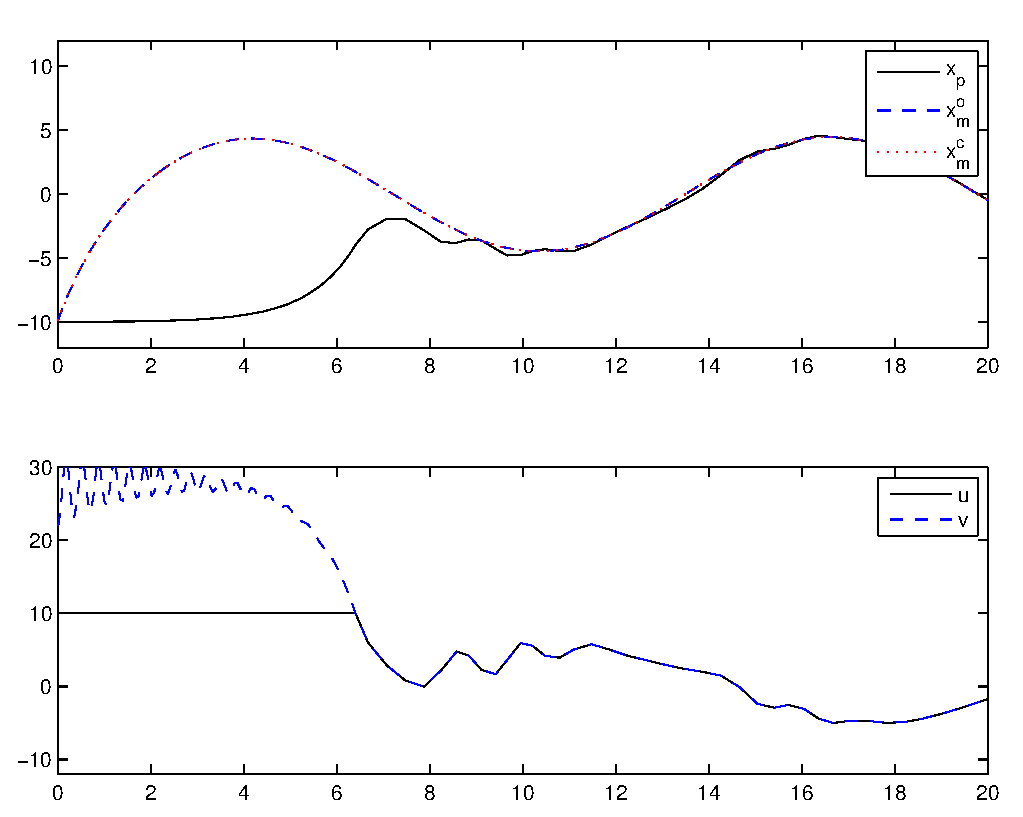
\includegraphics[width=3.0in]{\figurepath/fig1orm.eps}
    \caption{ORM:\ State and input}
  \end{center}
\end{figure}

\begin{figure}[H]
  \begin{center}
    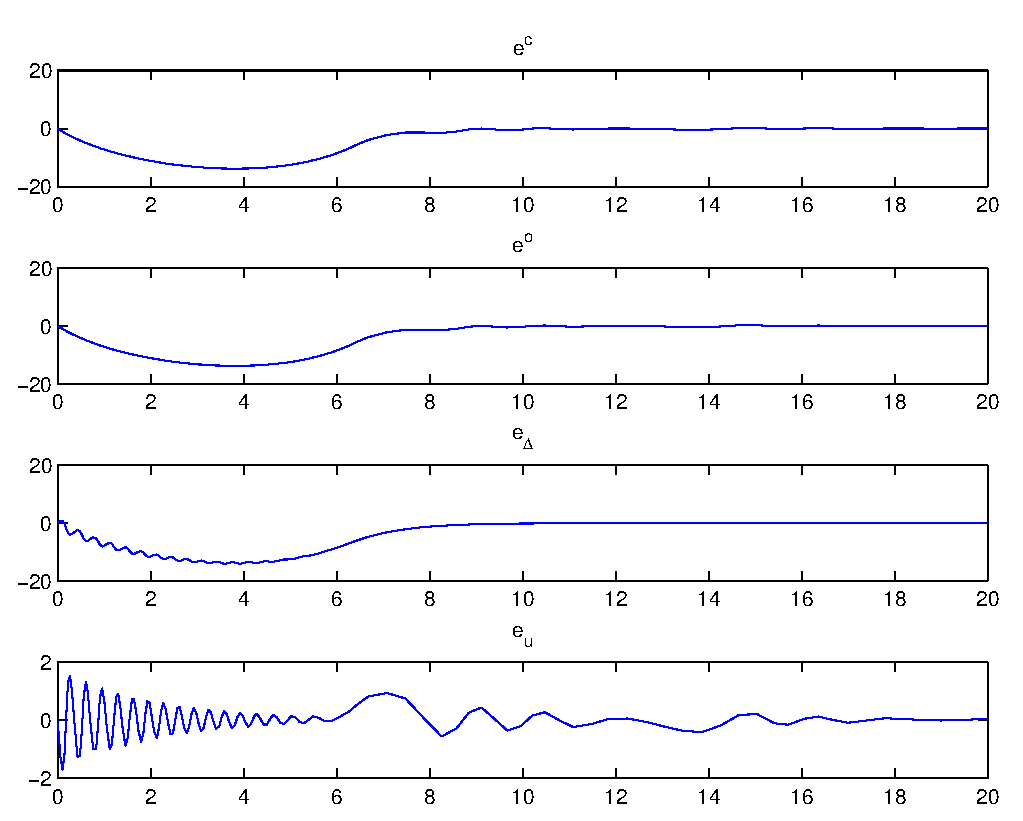
\includegraphics[width=3.0in]{\figurepath/fig2orm.eps}
    \caption{ORM:\ errors}
  \end{center}
\end{figure}

\begin{figure}[H]
  \begin{center}
    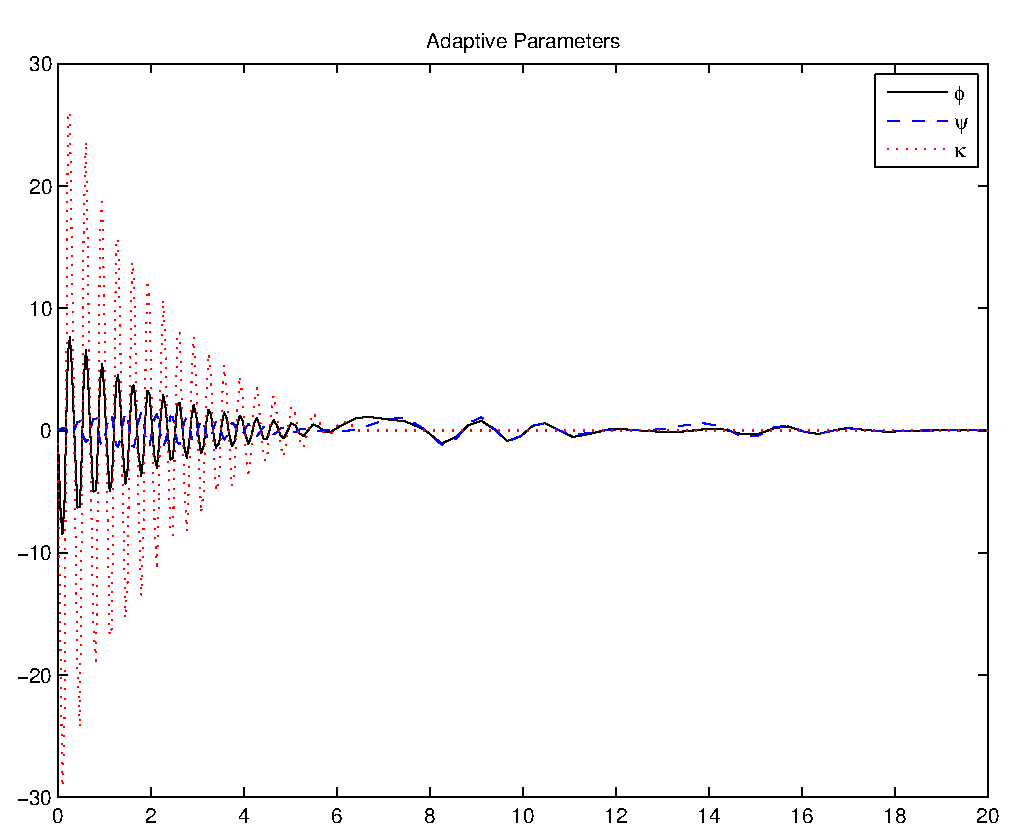
\includegraphics[width=3.0in]{\figurepath/fig3orm.eps}
    \caption{ORM:\ Parameters}
  \end{center}
\end{figure}

\subsection{Extension to Closed-Loop Reference Model}

Setting $\ell=0$ recovers the normal open-loop reference model case.
\begin{equation*}
  \dot{e}_{\Delta}=(a_{m}+\ell)e_{\Delta}+\beta_{\Delta}\Delta u
\end{equation*}
When the control input is saturating, the controller cannot achieve any higher level of performance.
That is, the controller should not seek to minimize an error signal which it is unable to do because of the limitation of the actuator.
Instead we define the error $e_{u}$ which takes the state error (the actual error we would like to minimize) and subtracts off the portion of the error due to the ``disturbance'' $\Delta u$ which the controller input can do nothing about.
This is the error we would like to use to drive adaptation.
If the controller is causing the input to saturate, there is no sense using an error signal which the controller cannot reduce to drive adaptation.
\begin{equation*}
  e_{u}=e^{c}-e_{\Delta}
\end{equation*}
The dynamics describing this error are given by
\begin{equation*}
  \dot{e}_{u}=\dot{e}^{c}-\dot{e}_{\Delta}
\end{equation*}
where, differentiating the state error
\begin{equation*}
  \dot{e}^{c}=\dot{x}_{p}-\dot{x}_{m}^{c}
\end{equation*}
plugging in
\begin{equation*}
  \dot{e}^{c}=a_{p}x_{p}+b_{p}u-a_{m}x_{m}^{c}-b_{m}r+\ell(x_{p}-x_{m}^{c})
\end{equation*}
Substituting in the control law $u=u_{c}+\Delta u$ and the matching conditions $a_{p}=a_{m}-b_{p}\theta^{*}$ and $b_{m}=b_{p}k^{*}$ we get
\begin{equation*}
  \dot{e}^{c}=(a_{m}-b_{p}\theta^{*})x_{p}+b_{p}(u_{c}+\Delta u)-a_{m}x_{m}^{c}-b_{p}k^{*}r+\ell(x_{p}-x_{m}^{c})
\end{equation*}
and then
\begin{equation*}
  \dot{e}^{c}=a_{m}x_{p}-b_{p}\theta^{*}x_{p}+b_{p}u_{c}+b_{p}\Delta u-a_{m}x_{m}^{c}-b_{p}k^{*}r+\ell x_{p}-\ell x_{m}^{c}
\end{equation*}
and then
\begin{equation*}
  \dot{e}^{c}=(a_{m}+\ell)(x_{p}-x_{m}^{c})-b_{p}\theta^{*}x_{p}+b_{p}u_{c}+b_{p}\Delta u-b_{p}k^{*}r
\end{equation*}
and now substituting the control law $u_{c}=\theta x_{p}+kr$ in
\begin{equation*}
  \dot{e}^{c}=(a_{m}+\ell)e^{c}-b_{p}\theta^{*}x_{p}+b_{p}\theta x_{p}+b_{p}kr+b_{p}\Delta u-b_{p}k^{*}r
\end{equation*}
and then
\begin{equation*}
  \dot{e}^{c}=(a_{m}+\ell)e^{c}+b_{p}(\theta-\theta^{*})x_{p}+b_{p}(k-k^{*})r+b_{p}\Delta u
\end{equation*}
Now define the following parameter errors
\begin{empheq}[box=\roomyfbox]{equation*}
  \tilde{\theta}=\theta-\theta^{*}
\end{empheq}
\begin{empheq}[box=\roomyfbox]{equation*}
  \tilde{k}=k-k^{*}
\end{empheq}
and substituting these in
\begin{equation*}
  \dot{e}^{c}=(a_{m}+\ell)e^{c}+b_{p}\tilde{\theta}x_{p}+b_{p}\tilde{k}r+b_{p}\Delta u
\end{equation*}
Now returning to $\dot{e}_{u}$
\begin{equation*}
  \dot{e}_{u}=(a_{m}+\ell)e^{c}+b_{p}\tilde{\theta}x_{p}+b_{p}\tilde{k}r+b_{p}\Delta u-(a_{m}+\ell)e_{\Delta}-\beta_{\Delta}\Delta u
\end{equation*}
and then
\begin{equation*}
  \dot{e}_{u}=(a_{m}+\ell)e_{u}+b_{p}\tilde{\theta}x_{p}+b_{p}\tilde{k}r+(b_{p}-\beta_{\Delta})\Delta u
\end{equation*}
and define the last parameter
\begin{empheq}[box=\roomyfbox]{equation*}
  \tilde{\beta}=b_{p}-\beta_{\Delta}
\end{empheq}
and then
\begin{equation*}
  \dot{e}_{u}=(a_{m}+\ell)e_{u}+b_{p}\tilde{\theta}x_{p}+b_{p}\tilde{k}r+\tilde{\beta}\Delta u
\end{equation*}
This is the error we want to try to minimize.
Now propose the following candidate Lyapunov function
\begin{empheq}[box=\roomyfbox]{equation*}
  V(e_{u},\tilde{\theta},\tilde{k},\tilde{\beta})=
  \frac{1}{2}e_{u}{}^{2}+
  \frac{1}{2}|b_{p}|\gamma_{1}^{-1}\tilde{\theta}^{2}+
  \frac{1}{2}|b_{p}|\gamma_{2}^{-1}\tilde{k}^{2}+
  \frac{1}{2}\gamma_{3}^{-1}\tilde{\beta}^{2}
\end{empheq}
taking the time derivative
\begin{equation*}
  \dot{V}=e_{u}\dot{e}_{u}+
  |b_{p}|\gamma_{1}^{-1}\tilde{\theta}\dot{\tilde{\theta}}+
  |b_{p}|\gamma_{2}^{-1}\tilde{k}\dot{\tilde{k}}+
  \gamma_{3}^{-1}\tilde{\beta}\dot{\tilde{\beta}}
\end{equation*}
substituting in $\dot{e}_{u}$
\begin{equation*}
  \dot{V}=e_{u}[(a_{m}+\ell)e_{u}+b_{p}\tilde{\theta}x_{p}+b_{p}\tilde{k}r+\tilde{\beta}\Delta u]+
  |b_{p}|\gamma_{1}^{-1}\tilde{\theta}\dot{\tilde{\theta}}+
  |b_{p}|\gamma_{2}^{-1}\tilde{k}\dot{\tilde{k}}+
  \gamma_{3}^{-1}\tilde{\beta}\dot{\tilde{\beta}}
\end{equation*}
and then
\begin{equation*}
  \dot{V}=(a_{m}+\ell)e_{u}{}^{2}+b_{p}\tilde{\theta}e_{u}x_{p}+b_{p}\tilde{k}e_{u}r+\tilde{\beta}e_{u}\Delta u+
  |b_{p}|\gamma_{1}^{-1}\tilde{\theta}\dot{\tilde{\theta}}+
  |b_{p}|\gamma_{2}^{-1}\tilde{k}\dot{\tilde{k}}+
  \gamma_{3}^{-1}\tilde{\beta}\dot{\tilde{\beta}}
\end{equation*}
Now the goal is to determine adaptive update laws for each of the parameters $\tilde{\theta}$, $\tilde{k}$, and $\tilde{\beta}$ such that all of the terms except the quadratic in $e_{u}$ are left.
That is
\begin{align*}
  b_{p}\tilde{\theta}e_{u}x_{p}+|b_{p}|\gamma_{1}^{-1}\tilde{\theta}\dot{\tilde{\theta}}=&0 \\
  b_{p}\tilde{k}e_{u}r+|b_{p}|\gamma_{2}^{-1}\tilde{k}\dot{\tilde{k}}=&0 \\
  \tilde{\beta}e_{u}\Delta u+\gamma_{3}^{-1}\tilde{\beta}\dot{\tilde{\beta}}=&0
\end{align*}
So this results in the following update laws
\begin{align*}
  \dot{\tilde{\theta}}&=-\gamma_{1}\text{sgn}(b_{p})e_{u}x_{p} \\
  \dot{\tilde{k}}&=-\gamma_{2}\text{sgn}(b_{p})e_{u}r \\
  \dot{\tilde{\beta}}&=-\gamma_{3}e_{u}\Delta u
\end{align*}
resulting in the following time derivative $\dot{V}$
\begin{equation*}
  \dot{V}=(a_{m}+\ell)e_{u}{}^{2}\leq0
\end{equation*}
And with $\dot{V}$ negative semi-definite, then $V$ is bounded above by $V(t_{0})$ and below by zero.
Additionally, the arguments of $V$ are also bounded for all $t\geq t_{0}$.

\subsubsection{Simulation Results}

\begin{figure}[H]
  \begin{center}
    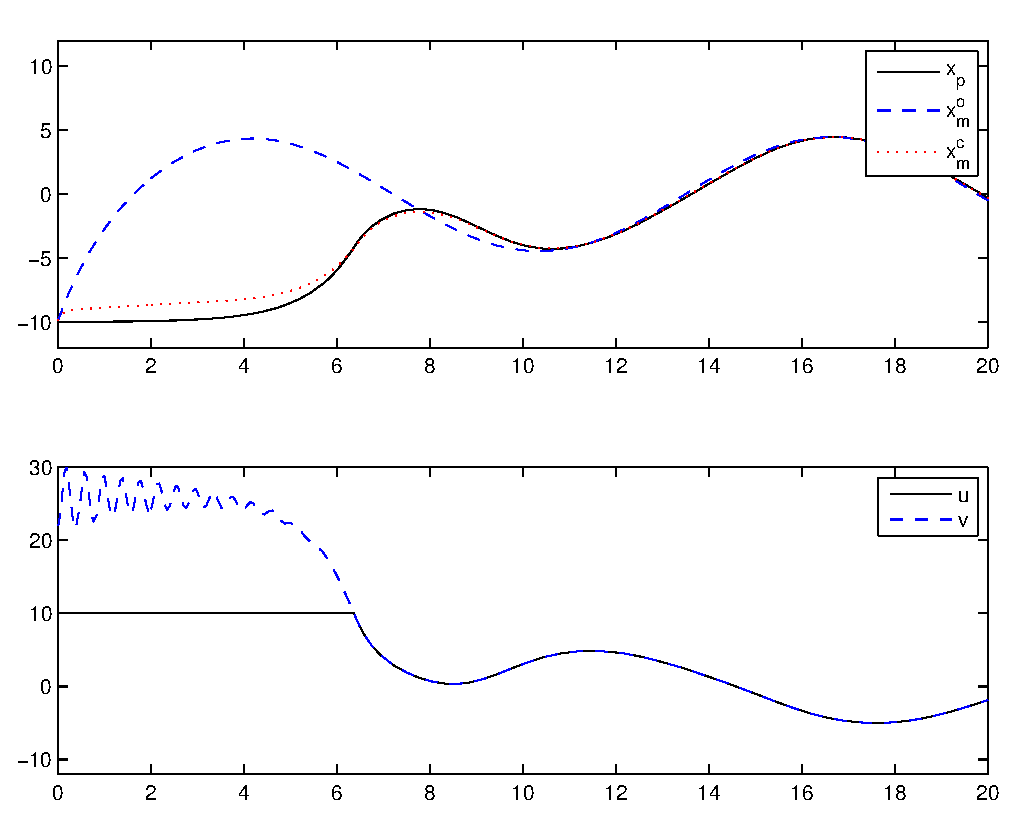
\includegraphics[width=3.0in]{\figurepath/fig1crm.eps}
    \caption{CRM:\ State and input}
  \end{center}
\end{figure}

\begin{figure}[H]
  \begin{center}
    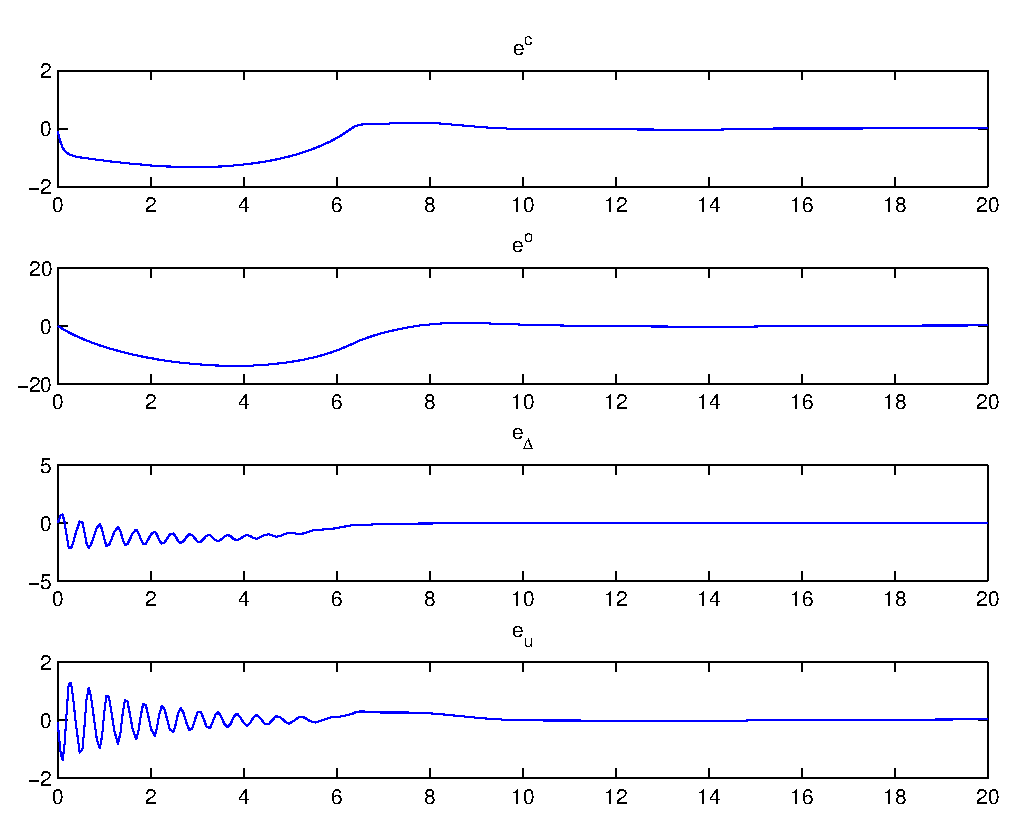
\includegraphics[width=3.0in]{\figurepath/fig2crm.eps}
    \caption{CRM:\ errors}
  \end{center}
\end{figure}

\begin{figure}[H]
  \begin{center}
    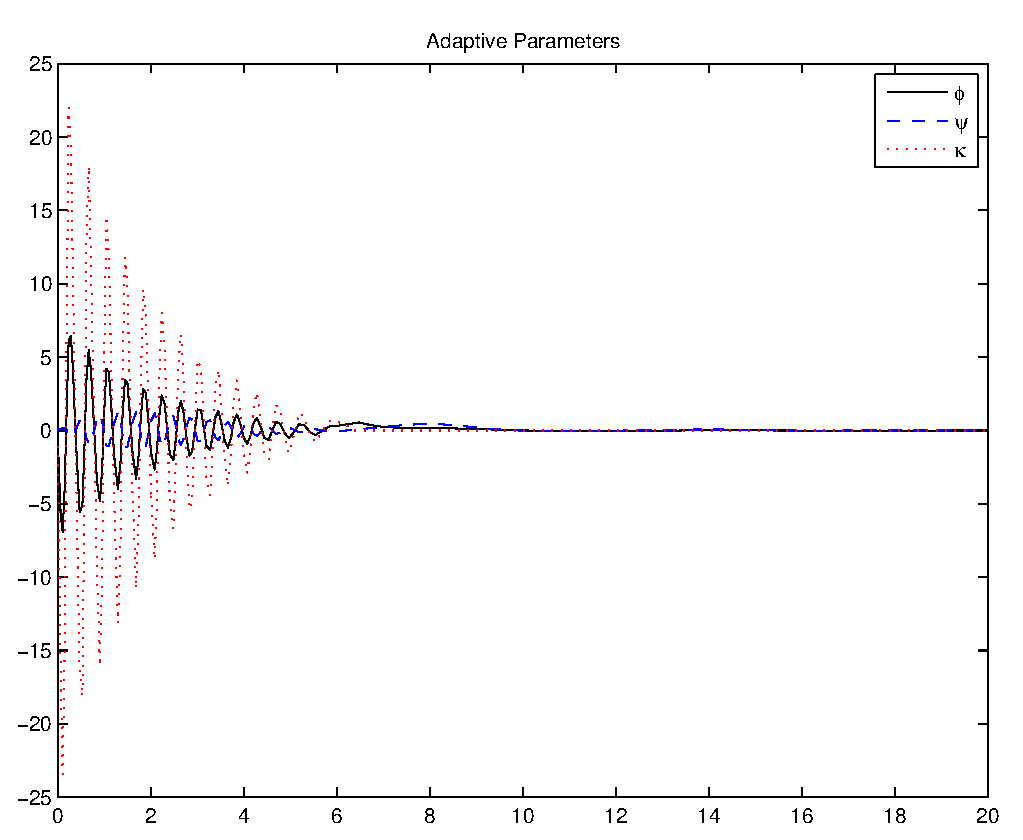
\includegraphics[width=3.0in]{\figurepath/fig3crm.eps}
    \caption{CRM:\ Parameters}
  \end{center}
\end{figure}

\subsection{Saturation Protection Higher Order with CRM}

Plant to be controlled
\begin{equation*}
  \dot{x}=(A+B_{1}\Lambda W^{\mathsf{T}})x+B_{1}\Lambda u+B_{2}x_{\text{cmd}}
\end{equation*}
commanded control law
\begin{equation*}
  u_{c}=(\theta+K_{x})^{\mathsf{T}}x
\end{equation*}
actual control input to the plant due to the position saturation of the actuators
\begin{equation*}
  u=
  \begin{cases}
    u_{c} &\mbox{if } |u_{c}|\leq u_{\text{max}} \\
    u_{\text{max}}\text{sgn}(u_{c}) & \mbox{if } |u_{c}|>u_{\text{max}}
  \end{cases}
\end{equation*}
$\Delta u$ is the control deficit.
\begin{empheq}[box=\roomyfbox]{equation*}
  u=u_{c}+\Delta{} u
\end{empheq}
Plugging in the control into the plant equation and $r=x_{\text{cmd}}$
\begin{equation*}
  \dot{x}=(A+B_{1}\Lambda W^{\mathsf{T}})x+B_{1}\Lambda(u_{c}+\Delta u)+B_{2}r
\end{equation*}
and then
\begin{equation*}
  \dot{x}=(A+B_{1}\Lambda W^{\mathsf{T}})x+B_{1}\Lambda u_{c}+B_{1}\Lambda\Delta u+B_{2}r
\end{equation*}
The reference model is given by
\begin{equation*}
  \dot{x}_{m}^{c}=A_{m}x_{m}^{c}+B_{m}x_{\text{cmd}}-L(x-x_{m}^{c})
\end{equation*}
\begin{equation*}
  \dot{x}_{m}^{c}=A_{m}x_{m}^{c}+B_{2}r-L(x-x_{m}^{c})
\end{equation*}
where
\begin{equation*}
  A_{m}=A+B_{1}K_{x}^{\mathsf{T}}
\end{equation*}
I am using a closed-loop reference model
\begin{empheq}[box=\roomyfbox]{equation*}
  \dot{e}_{\Delta}=(A_{m}+L)e_{\Delta}+\beta_{\Delta}\Delta{} u
\end{empheq}
and
\begin{empheq}[box=\roomyfbox]{equation*}
  e_{u}=e^{c}-e_{\Delta}
\end{empheq}
The dynamics describing this error are given by
\begin{equation*}
  \dot{e}_{u}=\dot{e}^{c}-\dot{e}_{\Delta}
\end{equation*}
where, differentiating the state error
\begin{equation*}
  \dot{e}^{c}=\dot{x}-\dot{x}_{m}^{c}
\end{equation*}
plugging in
\begin{equation*}
  \dot{e}^{c}=(A+B_{1}\Lambda W^{\mathsf{T}})x+B_{1}\Lambda u_{c}+B_{1}\Lambda\Delta u+B_{2}r-
  [A_{m}x_{m}^{c}+B_{2}r-L(x-x_{m}^{c})]
\end{equation*}
and then
\begin{equation*}
  \dot{e}^{c}=(A+B_{1}\Lambda W^{\mathsf{T}})x+B_{1}\Lambda u_{c}+B_{1}\Lambda\Delta u-
  A_{m}x_{m}^{c}+L(x-x_{m}^{c})
\end{equation*}
Using $A=A_{m}-B_{1}K_{x}^{\mathsf{T}}$ and $u_{c}=(\theta+K_{x})^{\mathsf{T}}x$
\begin{equation*}
  \dot{e}^{c}=(A_{m}-B_{1}K_{x}^{\mathsf{T}}+B_{1}\Lambda W^{\mathsf{T}})x+B_{1}\Lambda(\theta+K_{x})^{\mathsf{T}}x+B_{1}\Lambda\Delta u-
  A_{m}x_{m}^{c}+L(x-x_{m}^{c})
\end{equation*}
and then
\begin{equation*}
  \dot{e}^{c}=A_{m}x+(-B_{1}K_{x}^{\mathsf{T}}+B_{1}\Lambda W^{\mathsf{T}})x+B_{1}\Lambda\theta^{\mathsf{T}}x+B_{1}\Lambda K_{x}^{\mathsf{T}}x+B_{1}\Lambda\Delta u-A_{m}x_{m}^{c}+L(x-x_{m}^{c})
\end{equation*}
and then
\begin{equation*}
  \dot{e}^{c}=A_{m}(x-x_{m}^{c})+(B_{1}\Lambda\theta^{\mathsf{T}}+B_{1}\Lambda K_{x}^{\mathsf{T}}-B_{1}K_{x}^{\mathsf{T}}+B_{1}\Lambda W^{\mathsf{T}})x+B_{1}\Lambda\Delta u+L(x-x_{m}^{c})
\end{equation*}
and then
\begin{equation*}
  \dot{e}^{c}=(A_{m}+L)(x-x_{m}^{c})+(B_{1}\Lambda\theta^{\mathsf{T}}+B_{1}\Lambda K_{x}^{\mathsf{T}}-B_{1}K_{x}^{\mathsf{T}}+B_{1}\Lambda W^{\mathsf{T}})x+B_{1}\Lambda\Delta u
\end{equation*}
and then
\begin{equation*}
  \dot{e}^{c}=(A_{m}+L)(x-x_{m}^{c})+B_{1}(\Lambda\theta^{\mathsf{T}}+\Lambda K_{x}^{\mathsf{T}}-K_{x}^{\mathsf{T}}+\Lambda W^{\mathsf{T}})x+B_{1}\Lambda\Delta u
\end{equation*}
and from the matching condition we have
\begin{equation*}
  \Lambda\left[W^{\mathsf{T}}+(\theta^{*}+K_{x})^{\mathsf{T}}\right]=K_{x}^{\mathsf{T}}
\end{equation*}
which we can rearrange
\begin{equation*}
  \Lambda W^{\mathsf{T}}+\Lambda\theta^{*\mathsf{T}}+\Lambda K_{x}^{\mathsf{T}}=K_{x}^{\mathsf{T}}
\end{equation*}
and then
\begin{equation*}
  \Lambda K_{x}^{\mathsf{T}}-K_{x}^{\mathsf{T}}+\Lambda W^{\mathsf{T}}=-\Lambda\theta^{*\mathsf{T}}
\end{equation*}
substituting this in
\begin{equation*}
  \dot{e}^{c}=(A_{m}+L)(x-x_{m}^{c})+B_{1}(\Lambda\theta^{\mathsf{T}}-\Lambda\theta^{*\mathsf{T}})x+B_{1}\Lambda\Delta u
\end{equation*}
and with $\tilde{\theta}=\theta-\theta^{*}$ we get
\begin{equation*}
  \dot{e}^{c}=(A_{m}+L)(x-x_{m}^{c})+B_{1}\Lambda\tilde{\theta}^{\mathsf{T}}x+B_{1}\Lambda\Delta u
\end{equation*}
\begin{equation*}
  \dot{e}^{c}=(A_{m}+L)e^{c}+B_{1}\Lambda\tilde{\theta}^{\mathsf{T}}x+B_{1}\Lambda\Delta u
\end{equation*}
And using $\dot{e}_{u}=\dot{e}^{c}-\dot{e}_{\Delta}$
\begin{equation*}
  \dot{e}_{u}=(A_{m}+L)e^{c}+B_{1}\Lambda\tilde{\theta}^{\mathsf{T}}x+B_{1}\Lambda\Delta u-
  [(A_{m}+L)e_{\Delta}+\beta_{\Delta}\Delta u]
\end{equation*}
and then
\begin{equation*}
  \dot{e}_{u}=(A_{m}+L)e^{c}+B_{1}\Lambda\tilde{\theta}^{\mathsf{T}}x+B_{1}\Lambda\Delta u-
  (A_{m}+L)e_{\Delta}-\beta_{\Delta}\Delta u
\end{equation*}
and then
\begin{equation*}
  \dot{e}_{u}=(A_{m}+L)(e^{c}-e_{\Delta})+B_{1}\Lambda\tilde{\theta}^{\mathsf{T}}x+B_{1}\Lambda\Delta u-\beta_{\Delta}\Delta u
\end{equation*}
and then
\begin{equation*}
  \dot{e}_{u}=(A_{m}+L)e_{u}+B_{1}\Lambda\tilde{\theta}^{\mathsf{T}}x+(B_{1}\Lambda-\beta_{\Delta})\Delta u
\end{equation*}
defining $\tilde{\beta}=B_{1}\Lambda-\beta_{\Delta}$ we get the following augmented error dynamics
\begin{equation*}
  \dot{e}_{u}=(A_{m}+L)e_{u}+B_{1}\Lambda\tilde{\theta}^{\mathsf{T}}x+\tilde{\beta}\Delta u
\end{equation*}
\begin{empheq}[box=\roomyfbox]{equation*}
  \dot{e}_{u}=\bar{A}_{m}e_{u}+B_{1}\Lambda\tilde{\theta}^{\mathsf{T}}x+\tilde{\beta}\Delta{} u
\end{empheq}
Proposing the following candidate Lyapunov function
\begin{empheq}[box=\roomyfbox]{equation*}
  V=e_{u}^{\mathsf{T}}Pe_{u}+
  \text{tr}\left(\tilde{\theta}^{\mathsf{T}}\Gamma^{-1}\tilde{\theta}|\Lambda|\right)+
  \tilde{\beta}^{\mathsf{T}}\Gamma_{\beta}^{-1}\tilde{\beta}
\end{empheq}
Differentiating
\begin{equation*}
  \dot{V}={\dot{e}}_{u}^{\mathsf{T}}Pe_{u}+e_{u}^{\mathsf{T}}P\dot{e}_{u}+
  \text{tr}(\dot{\tilde{\theta}}^{\mathsf{T}}\Gamma^{-1}\tilde{\theta}|\Lambda|)+
  \text{tr}({\tilde{\theta}}^{\mathsf{T}}\Gamma^{-1}\dot{\tilde{\theta}}|\Lambda|)+
  \dot{\tilde{\beta}}^{\mathsf{T}}\Gamma_{\beta}^{-1}\tilde{\beta}+
  \tilde{\beta}^{\mathsf{T}}\Gamma_{\beta}^{-1}\dot{\tilde{\beta}}
\end{equation*}
Substituting error dynamics equation from above, with the transpose
\begin{equation*}
  \dot{e}_{u}^{\mathsf{T}}=e_{u}^{\mathsf{T}}\bar{A}_{m}^{\mathsf{T}}+x^{\mathsf{T}}\tilde{\theta}\Lambda B_{1}^{\mathsf{T}}+\Delta u^{\mathsf{T}}\tilde{\beta}^{\mathsf{T}}
\end{equation*}
and simplifying
\begin{equation*}
  \dot{V}
  =(e_{u}^{\mathsf{T}}\bar{A}_{m}^{\mathsf{T}}+x^{\mathsf{T}}\tilde{\theta}\Lambda B_{1}^{\mathsf{T}}
  +\Delta u^{\mathsf{T}}\tilde{\beta}^{\mathsf{T}})Pe_{u}+e_{u}^{\mathsf{T}}P(\bar{A}_{m}e_{u}
  +B_{1}\Lambda\tilde{\theta}^{\mathsf{T}}x+\tilde{\beta}\Delta u)
  +\text{tr}(\dot{\tilde{\theta}}^{\mathsf{T}}\Gamma^{-1}\tilde{\theta}|\Lambda|)
  +\text{tr}({\tilde{\theta}}^{\mathsf{T}}\Gamma^{-1}\dot{\tilde{\theta}}|\Lambda|)
  +\dot{\tilde{\beta}}^{\mathsf{T}}\Gamma_{\beta}^{-1}\tilde{\beta}
  +\tilde{\beta}^{\mathsf{T}}\Gamma_{\beta}^{-1}\dot{\tilde{\beta}}
\end{equation*}
and then
\begin{equation*}
  \dot{V}=(e_{u}^{\mathsf{T}}\bar{A}_{m}^{\mathsf{T}}Pe_{u})+
  (x^{\mathsf{T}}\tilde{\theta}\Lambda B_{1}^{\mathsf{T}}+\Delta u^{\mathsf{T}}\tilde{\beta}^{\mathsf{T}})Pe_{u}+
  (e_{u}^{\mathsf{T}}P\bar{A}_{m}e_{u})+
  e_{u}^{\mathsf{T}}P(B_{1}\Lambda\tilde{\theta}^{\mathsf{T}}x+\tilde{\beta}\Delta u)+
  \text{tr}(\dot{\tilde{\theta}}^{\mathsf{T}}\Gamma^{-1}\tilde{\theta}|\Lambda|)+
  \text{tr}({\tilde{\theta}}^{\mathsf{T}}\Gamma^{-1}\dot{\tilde{\theta}}|\Lambda|)+
  \dot{\tilde{\beta}}^{\mathsf{T}}\Gamma_{\beta}^{-1}\tilde{\beta}+
  \tilde{\beta}^{\mathsf{T}}\Gamma_{\beta}^{-1}\dot{\tilde{\beta}}
\end{equation*}
and then
\begin{equation*}
  \dot{V}=e_{u}^{\mathsf{T}}(\bar{A}_{m}^{\mathsf{T}}P+P\bar{A}_{m})e_{u}+
  (x^{\mathsf{T}}\tilde{\theta}\Lambda B_{1}^{\mathsf{T}}+\Delta u^{\mathsf{T}}\tilde{\beta}^{\mathsf{T}})Pe_{u}+
  e_{u}^{\mathsf{T}}P(B_{1}\Lambda\tilde{\theta}^{\mathsf{T}}x+\tilde{\beta}\Delta u)+
  \text{tr}(\dot{\tilde{\theta}}^{\mathsf{T}}\Gamma^{-1}\tilde{\theta}|\Lambda|)+
  \text{tr}({\tilde{\theta}}^{\mathsf{T}}\Gamma^{-1}\dot{\tilde{\theta}}|\Lambda|)+
  \dot{\tilde{\beta}}^{\mathsf{T}}\Gamma_{\beta}^{-1}\tilde{\beta}+
  \tilde{\beta}^{\mathsf{T}}\Gamma_{\beta}^{-1}\dot{\tilde{\beta}}
\end{equation*}
and with $\bar{A}_{m}^{\mathsf{T}}P+P\bar{A}_{m}=-Q$ we get
\begin{equation*}
  \dot{V}=-e_{u}^{\mathsf{T}}Qe_{u}+
  x^{\mathsf{T}}\tilde{\theta}\Lambda B_{1}^{\mathsf{T}}Pe_{u}+
  \Delta u^{\mathsf{T}}\tilde{\beta}^{\mathsf{T}}Pe_{u}+
  e_{u}^{\mathsf{T}}PB_{1}\Lambda\tilde{\theta}^{\mathsf{T}}x+
  e_{u}^{\mathsf{T}}P\tilde{\beta}\Delta u+
  \text{tr}(\dot{\tilde{\theta}}^{\mathsf{T}}\Gamma^{-1}\tilde{\theta}|\Lambda|)+
  \text{tr}({\tilde{\theta}}^{\mathsf{T}}\Gamma^{-1}\dot{\tilde{\theta}}|\Lambda|)+
  \dot{\tilde{\beta}}^{\mathsf{T}}\Gamma_{\beta}^{-1}\tilde{\beta}+
  \tilde{\beta}^{\mathsf{T}}\Gamma_{\beta}^{-1}\dot{\tilde{\beta}}
\end{equation*}
since the terms of $\dot{V}$ are all scalars we have
\begin{equation*}
  \dot{V}=-e_{u}^{\mathsf{T}}Qe_{u}+
  2x^{\mathsf{T}}\tilde{\theta}\Lambda B_{1}^{\mathsf{T}}Pe_{u}+
  2 \Delta u^{\mathsf{T}}\tilde{\beta}^{\mathsf{T}}Pe_{u}+
  \text{tr}(\dot{\tilde{\theta}}^{\mathsf{T}}\Gamma^{-1}\tilde{\theta}|\Lambda|)+
  \text{tr}({\tilde{\theta}}^{\mathsf{T}}\Gamma^{-1}\dot{\tilde{\theta}}|\Lambda|)+
  2\tilde{\beta}^{\mathsf{T}}\Gamma_{\beta}^{-1}\dot{\tilde{\beta}}
\end{equation*}
The following adaptive control gain update laws are proposed
\begin{empheq}[box=\roomyfbox]{equation*}
  \dot{\theta}=\text{Proj}_{\Gamma}(\theta,-\Gamma{} xe_{u}^{\mathsf{T}}PB_{1}\text{sgn}(\Lambda))
\end{empheq}
\begin{empheq}[box=\roomyfbox]{equation*}
  \dot{\tilde{\beta}}=-\Gamma_{\beta}Pe_{u}\Delta{} u
\end{empheq}
Looking at only the $\tilde{\beta}$ terms
\begin{equation*}
  2 \Delta u^{\mathsf{T}}\tilde{\beta}^{\mathsf{T}}Pe_{u}-
  2\tilde{\beta}^{\mathsf{T}}\Gamma_{\beta}^{-1}\Gamma_{\beta}Pe_{u}\Delta u=
\end{equation*}
and since we are considering scalar input system
\begin{equation*}
  2 \Delta u^{\mathsf{T}}\tilde{\beta}^{\mathsf{T}}Pe_{u}-
  2\Delta u \tilde{\beta}^{\mathsf{T}}Pe_{u}=0
\end{equation*}
and so $\dot{V}$ becomes
\begin{equation*}
  \dot{V}=-e_{u}^{\mathsf{T}}Qe_{u}+
  2x^{\mathsf{T}}\tilde{\theta}\Lambda B_{1}^{\mathsf{T}}Pe_{u}+
  \text{tr}(\dot{\tilde{\theta}}^{\mathsf{T}}\Gamma^{-1}\tilde{\theta}|\Lambda|)+
  \text{tr}({\tilde{\theta}}^{\mathsf{T}}\Gamma^{-1}\dot{\tilde{\theta}}|\Lambda|)
\end{equation*}
using $\text{tr}(a)=\text{tr}(a^{\mathsf{T}})$, $\Lambda=\Lambda^{\mathsf{T}}$, $\Gamma=\Gamma^{\mathsf{T}}$, and $\text{tr}(ab)=\text{tr}(ba)$ we get
\begin{equation*}
  \dot{V}=-e_{u}^{\mathsf{T}}Qe+2x^{\mathsf{T}}{\tilde{\theta}}\Lambda{B_{1}}^{\mathsf{T}}Pe_{u}
  +2\text{tr}({\tilde{\theta}}^{\mathsf{T}}\Gamma^{-1}\dot{\tilde{\theta}}|\Lambda|) \\
\end{equation*}
Substituting the adaptive control gain update law for $\theta$
\begin{equation*}
  \dot{V}=-e_{u}^{\mathsf{T}}Qe+2x^{\mathsf{T}}{\tilde{\theta}}\Lambda{B_{1}}^{\mathsf{T}}Pe_{u}
  +2\text{tr}\left({\tilde{\theta}}^{\mathsf{T}}\Gamma^{-1}\text{Proj}_{\Gamma}(\theta,-\Gamma xe_{u}^{\mathsf{T}}PB_{1}\text{sgn}(\Lambda))|\Lambda|\right) \\
\end{equation*}
Since the quantity $2x^{\mathsf{T}}{\tilde{\theta}}\Lambda{B_{1}}^{\mathsf{T}}Pe_{u}$ is scalar, it is equal to its trace, so we can write
\begin{equation*}
  \dot{V}=-e_{u}^{\mathsf{T}}Qe_{u}+2\text{tr}(x^{\mathsf{T}}{\tilde{\theta}}\Lambda{B_{1}}^{\mathsf{T}}Pe_{u})
  +2\text{tr}\left({\tilde{\theta}}^{\mathsf{T}}\Gamma^{-1}\text{Proj}_{\Gamma}(\theta,-\Gamma xe_{u}^{\mathsf{T}}PB_{1}\text{sgn}(\Lambda))|\Lambda|\right) \\
\end{equation*}
The terms inside the first trace operator can be rearranged using $\text{tr}(a)=\text{tr}(a^{\mathsf{T}})$, $\Lambda=\Lambda^{\mathsf{T}}$, and $\text{tr}(ab)=\text{tr}(ba)$
\begin{equation*}
  \dot{V}=-e_{u}^{\mathsf{T}}Qe_{u}+2\text{tr}(\tilde{\theta}^{\mathsf{T}}xe_{u}^{\mathsf{T}}PB_{1}\Lambda)
  +2\text{tr}\left({\tilde{\theta}}^{\mathsf{T}}\Gamma^{-1}\text{Proj}_{\Gamma}(\theta,-\Gamma xe_{u}^{\mathsf{T}}PB_{1}\text{sgn}(\Lambda))|\Lambda|\right) \\
\end{equation*}
Combining the trace operators
\begin{equation*}
  \dot{V}=-e_{u}^{\mathsf{T}}Qe_{u}
  +2\text{tr}\left(\tilde{\theta}^{\mathsf{T}}xe^{\mathsf{T}}PB_{1}\Lambda+
  {\tilde{\theta}}^{\mathsf{T}}\Gamma^{-1}\text{Proj}_{\Gamma}(\theta,-\Gamma xe_{u}^{\mathsf{T}}PB_{1}\text{sgn}(\Lambda))|\Lambda|\right) \\
\end{equation*}
\begin{equation*}
  \dot{V}=-e_{u}^{\mathsf{T}}Qe_{u}
  +2\text{tr}\left(\tilde{\theta}^{\mathsf{T}}\left(\Gamma^{-1}\text{Proj}_{\Gamma}(\theta,-\Gamma xe_{u}^{\mathsf{T}}PB_{1}\text{sign}(\Lambda))|\Lambda|+xe_{u}^{\mathsf{T}}PB_{1}\Lambda\right)\right) \\
\end{equation*}
Let $y=-xe_{u}^{\mathsf{T}}PB_{1}\text{sign}(\Lambda)$ and with $\text{sign}(\Lambda)|\Lambda|=\Lambda$
\begin{equation*}
  \dot{V}=-e_{u}^{\mathsf{T}}Qe_{u}
  +2\text{tr}\left(\tilde{\theta}^{\mathsf{T}}\left(\Gamma^{-1}\text{Proj}_{\Gamma}(\theta,\Gamma y)|\Lambda|-y|\Lambda|\right)\right)
\end{equation*}
\begin{equation*}
  \dot{V}=-e_{u}^{\mathsf{T}}Qe_{u}
  +2\text{tr}\left(\tilde{\theta}^{\mathsf{T}}\left(\Gamma^{-1}\text{Proj}_{\Gamma}(\theta,\Gamma y)-y\right)|\Lambda|\right)
\end{equation*}
And we have the following inequality (See my personal notes)
\begin{equation*}
  \tilde{\theta}^{\mathsf{T}}(\Gamma^{-1}\text{Proj}_{\Gamma}(\theta,\Gamma y)-y)\leq 0
\end{equation*}
So, if a symmetric, positive definite matrix $P$ exists, which solves the Lyapunov equation $\bar{A}_{m}{}^{\mathsf{T}}P+P\bar{A}_{m}+Q=0$, where $Q$ is positive definite, then $\dot{V}=\dot{V}(e,\theta)\leq 0$ is negative semidefinite, and $V(e,\theta)$ serves as a valid Lyapunov function for this system.

\chapter{Appendix}

\begin{example}
\begin{center}
\begin{tikzpicture}[auto, scale=0.9, every node/.style={transform shape}, node distance=1.0cm, >=latex']
\node[input](input1){};
\node[tee, right of= input1, node distance=1.0cm](tee2){};
\node[tee, above of= tee2, node distance=1.5cm](tee3){};
\node[tee, below of= tee2, node distance=1.5cm](tee4){};
\node[tee, right of=tee4,node distance=0.0cm] (block1){};
\node[squareblock, right of= block1, node distance=2.0cm](sum1){\shortstack{Adaptive \\  Controller}};
\node[squareblock, right of=sum1,label=above:{},node distance=3.0cm] (block2){\shortstack{Plant}};
\node[squareblock, above of=block2,label=below:{},label=above:{},node distance=3.0cm] (block3){\shortstack{Reference \\ Model}};
\node[tee, left of= block3, node distance=2.0cm](sum3){};
\node[roundblock, above of=block2,node distance=1.5cm] (block4){$\Theta$};
\node[whitesum, right of= tee2,node distance=9.0cm](sum2){};
\node[roundblock, above of=sum2,node distance=3.0cm] (block5){$L$};
\node[output, right of=sum2, node distance=2.5cm](output1){};
%Draw
\draw[-](input1) -- node[near start]{$z_{\text{cmd}}$} node[pos=0.7] {} (tee2);
\draw[-](tee2) -- (tee3);
\draw[-](tee2) -- (tee4);
\draw[->](tee3) -- node[pos=0.9]{} (block3);
%\draw[-](sum3) -- (block3);
\draw[-](tee4) -- (block1);
\draw[->](block1) -- node[near end] {} (sum1);
\draw[->](sum1) -- (block2);
\draw[->](block3) -| node[near start]{$x_{m}$} node[pos=0.3,name=xm]{} node[near end] {$-$} (sum2);
\draw[->](block2) -| node[near start]{$x$} node[pos=0.3,name=xp]{} node[pos=0.9] {$+$} (sum2);
\draw[->](xm) |- (block4);
\draw[->](block4) -| node[pos=0.9]{} (sum1);
\draw[->](sum2) -- node[near end]{$e$} node[pos=0.5, name=e, below]{} (output1);
\draw[->](e) |- (block5);
\draw[->](block5) -| node[pos=0.9]{} (block3);
%%Adaptive Arrow
%\coordinate (arrow1) at ([xshift=-0.7cm,yshift=-0.7cm] block1);
%\coordinate (arrow2) at (block1.225);
%\coordinate (arrow3) at (block1.45);
%\coordinate (arrow4) at ([xshift=0.7cm,yshift=0.7cm] block1);
%\draw[-](arrow1) -- (arrow2);
%\draw[->](arrow3) -- (arrow4);
%Adaptive Arrow
\coordinate (arrow1) at ([xshift=-0.7cm,yshift=-0.7cm] block4);
\coordinate (arrow2) at (block4.225);
\coordinate (arrow3) at (block4.45);
\coordinate (arrow4) at ([xshift=0.7cm,yshift=0.7cm] block4);
\draw[-](arrow1) -- (arrow2);
\draw[->](arrow3) -- (arrow4);
\end{tikzpicture}
\end{center}
\end{example}


\section{Eugene Lecture}

Last class $n^{*}\geq2$

EUGENE STUFF

Linear Control
LQR (state feedback)
PID (classical, output)
H-inf (both)
Pole placement (state feedback)
LQG (LQG+kalman filter/estimator)

Nonlinear Control
SMC (variable structure control)
- good for DC motor control, bad for flight control
Feedback linearization (dynamic inversion, works great in Matlab, not good in real life\ldots
no guarantees for robustness)
Lyapunov redesign (mostly for systems with known dynamics, adaptive could kinda be considered to fall under here)
Adaptive control

all the control strategies above are model based design/analysis

Plant --> model
Models are all incorrect\ldots
Some more than others.
Use model to cook up control, hoping that even though model is incorrect the control will work on plant
Plant --> model --> controller

reason this works is robustness.
Robustness is the key.

Dynamic inversion very sensitive.
Dynamic inversion might work, but can take a lot of time to design analyze and tune.

$H_{\infty}$ control on Harrier\ldots

\begin{example}[X-45A]
  super unstable.
  Time to departure 20ms.
  3 gains in pitch
  5 gains in roll/yaw
  used LQR control.
\end{example}

pretty much everything Boeing does (80\textemdash{}90 percent) is LQR

Adaptive control.
Does it work? yes.
Does it always work? no!

build robust control (e.g.
LQR)

to fly all we need is 40* phase margin and 8dB gain margin.

LQR is really good for uncertainties in $A$ and $B$ but is highly sensitive when $A$ and $B$ are state dependent.
For example, standing shock wave on top of delta wing as it moves with changes in flight condition.

LQR controller has no tolerance to ``bubbles'' in, for example, pitching moment versus elevator angle plot because of shock wave.

\section{Dr.\ Annaswamy Lecturing}

SISO system

u to y through plant P

P is of form $W_{p}(s)=\frac{k_{p}Z_{p}(s)}{R_{p}(s)}$

degrees of freedom\ldots
Filters of dimension $n-1$

Error model

Introduce auxiliary error $e_{2}$, augmented error $\varepsilon_{1}$ where $\varepsilon_{1}=e_{1}+e_{2}$.
Use $\varepsilon_{1}$ instead of $e_{1}$ in adaptive law.

Omega in through $W_{m}(s)$ and get $\zeta$ then use $\dot{\theta}=-\varepsilon_{1}\zeta$

SHOW BLOCK DIAGRAM THAT GENERATES $e_{2}$.

BLOCK DIAGRAM FOR ANALYTIC PART, THAT ALGEBRAIC PART CANCELS

when $e_{1}+e_{2}$:\ $W_{m}(s)[\tilde{\theta}^{\top}]$ $+\tilde{\theta}^{\top}\zeta-W_{m}(s)[\tilde{\theta}^{\top}\omega]$ and assume for simplicity that $k^{*}=1$ and so we get $\varepsilon_{1}=\tilde{\theta}^{\top}\zeta$.
So now use $\dot{\tilde{\theta}}=-\varepsilon_{1}\zeta$.

Started out with adaptive system which was nonlinear and time-varying.
And $\tilde{\theta}$ is bounded so this is reduced to a linear time-varying system.
Can we then use this to prove stability? Need to take one more step.

Need to allow $\tilde{\theta}$ to grow slowly.
Make it the normalized quantity.

\section{Review}

Class review

control of an uncertain dynamic system:\ adaptive control

two bins:
\begin{enumerate}
  \setlength{\itemsep}{0pt}
  \item{Input, states, output}
  \item{parameters}
\end{enumerate}

in adaptive control measure as many of (1) as possible, and deal with as many in (2) as possible
must assume there is a plant model, and since parameters are being attached to the model, must assume the structure of the model is known

one unifying theme of adaptive control/identificaation:\ error model

Two classes of error:
\begin{enumerate}
  \setlength{\itemsep}{0pt}
  \item{parameter}
  \item{tracking}
\end{enumerate}

error model is ``black box'' between parameter error and tracking error.
Want this black box to have a nice feature to \ldots

\begin{enumerate}
  \setlength{\itemsep}{0pt}
  \item{error model 1:\ $e=\omega\tilde{\theta}$ $e$ is linear regression of $\tilde{\theta}$}
  \item{error model 2:\ dynamics between parameter error and $e$ $w=\omega\tilde{\theta}$ then $w$ goes into $\dot{e}=Ae+Bw$}
  \item{%
    error model 3:\ specific case of error model 2, and now only some part of the error is available $e_{1}$.
    And we needed dynamics to be SPR.\@
  }
  \item{error model 4:\ uses augmented error approach with adding and subtracting\ldots
  for arbitrary relative degree.
  Add $e_{1}$ and $e_{2}$ to get $\varepsilon_{1}$}
\end{enumerate}

Adaptive Control
(1) First order plant
$\frac{1}{s-a_{p}}$
so know model structure (its first order)
put $\theta$ in feedback
error model becomes $x_{p}$ -> $\tilde{\theta}$ -> $\frac{1}{s-a_{m}}$ -> $e$
$\dot{\tilde{\theta}}=-ex_{p}$

extend to $\frac{k_{p}}{s-a_{p}}$ where $k_{p}$ has known sign, by adding a feedforward part
error model becomes $\omega$ -> $\tilde{\theta}$ -> $\frac{k_{p}}{s-a_{m}}$ -> $e$
$\omega=[r x_{p}]^{\top}$
$\dot{\tilde{\theta}}=-sgn(k_{p})e\omega$

(2) States accessible
$\dot{x}_{p}=A_{p}x_{p}+Bu$
$B\Lambda^{*}=B_{m}$ where $\Lambda^{*}$ is diagonal with the sign of each of the elements on the diagonal is known.
$\omega=[r^{\top} x_{p}^{\top}]^{\top}$
$\omega$ -> $\tilde{\theta}$ -> box -> $e$
$\dot{\tilde{\theta}}=-sgn(\Lambda^{*})\omega e^{\top}PB_{m}$

Adaptive Control:\ PI, PID, Phase-Lead
popular for low order plant model
simple example:\ $\frac{1}{s(Js+B)}$
parameterization shown in class shows the dependence of control parameters on plant parameters

Relative degree 2
add $z$ into error model after $\tilde{\theta}$ and before dynamics where $z=\dot{\theta}^{\top}\bar{\omega}$
so $\bar{\omega}$ is a filtered version of $\omega$, and now we get error model $e$ in terms of this filtered $\omega$

$\dot{\tilde{\theta}}=-e\bar{\omega}$

\begin{tikzpicture}[thick]
  \node[draw,rectangle] (a) {A};
  \node[inner sep=0,minimum size=0,right of=a] (k) {}; % invisible node
  \node[draw,rectangle,right of=k] (b) {B};
  \node[draw,rectangle,below of=a] (c) {C};
  % 1st pass:\ draw arrows
  \draw[vecArrow] (a) to (b);
  \draw[vecArrow] (k) |- (c);
  % 2nd pass:\ copy all from 1st pass, and replace vecArrow with innerWhite
  \draw[innerWhite] (a) to (b);
  \draw[innerWhite] (k) |- (c);
  % Note:\ If you have no branches, the 2nd pass is not needed
\end{tikzpicture}

\begin{figure}[H]
  \begin{center}
    \begin{tikzpicture}[auto, scale=0.9, every node/.style={transform shape}, node distance=1.0cm, >=latex']
      \node[input](input1){};
      \node[tee, right of= input1,node distance=1.5cm](tee2){};
      \node[tee, above of= tee2,node distance=1.2cm](tee3){};
      \node[tee, below of= tee2,node distance=1.2cm](tee4){};
      \node[roundblock, right of=tee3,label=above:{},node distance=2.0cm] (block1){$\theta$};
      \node[roundblock, right of=tee4,label=above:{},node distance=2.0cm] (block2){$\hat{\theta}$};
      \node[output, right of= block1,node distance=1.5cm](output1){};
      \node[output, right of= block2,node distance=1.5cm](output2){};
      \draw[vecNoArrow](input1) -- node[near start]{$u$} node[pos=0.7] {} (tee2);
      \draw[vecArrow](tee2) |- (block1);
      \draw[vecArrow](tee2) |- (block2);
      \draw[->](block1) -- node[pos=0.7] {$y$} (output1);
      \draw[->](block2) -- node[pos=0.7] {$\hat{y}$} (output2);
      %\draw[innerWhite](input1) -- (tee2);
      %\draw[innerWhite](tee2) |- (block1);
      %\draw[innerWhite](tee2) |- (block2);
    \end{tikzpicture}
  \end{center}
\end{figure}


Extra block diagram
\begin{center}
  \begin{tikzpicture}[auto, scale=0.9, every node/.style={transform shape}, node distance=1.0cm, >=latex']
    \node[input](input1){};
    \node[roundblock, right of=input1,node distance=1.5cm] (block1){$a_{1}$};
    \node[whitesum, right of= block1, node distance=1.5cm](sum1){$+$};
    \node[squareblock, right of=sum1, node distance=2.0cm, minimum width=1.5cm] (block2){$\int$};
    \node[output, right of= block2, node distance=2.5cm](output1){};
    \node[roundblock, below of=block2,node distance=1.5cm] (block3){$a_{1}$};
    \draw[->](input1) -- (block1);
    \draw[->](block1) -- (sum1);
    \draw[->](sum1) -- (block2);
    \draw[->](block2) -- node[near end]{$x_{p}$} node[pos=0.5,name=xp]{} (output1);
    \draw[->](xp) |- (block3);
    \draw[->](block3) -| (sum1);
  \end{tikzpicture}
\end{center}

\subsection{Time Varying Parameters}

Consider the following time-varying plant, reference model, and control law
\begin{align*}
  \dot{x}_{p}&=a_{p}(t)x_{p}+u+d(t) \\
  \dot{x}_{m}&=a_{m}x_{m}+r \\
  u&=\theta x_{p}+r
\end{align*}
Gives time-varying matching condition

Lyapunov
\begin{equation*}
  V=\frac{1}{2}(e^{2}+\tilde{\theta}^{2})
\end{equation*}

\begin{equation*}
  \dot{V}=a_{m}e^{2}+\tilde{\theta}\dot{\tilde{\theta}}+\tilde{\theta}ex_{p}
\end{equation*}

\begin{equation*}
  \dot{V}=a_{m}e^{2}+\tilde{\theta}\dot{\theta}+\tilde{\theta}ex_{p}+\tilde{\theta}\dot{\theta}^{*}
\end{equation*}

Propose

\begin{equation*}
  \dot{\theta}=-ex_{p}-\sigma\theta
\end{equation*}

rewrite $\dot{V}$

\begin{equation*}
  \dot{V}=a_{m}e^{2}+\tilde{\theta}\dot{\theta}^{*}-\sigma\tilde{\theta}^{2}-\sigma\tilde{\theta}\theta^{*}(t)
\end{equation*}

if we know $|\theta^{*}(t)|\leq d_{1}$ and $|\dot{\theta}^{*}(t)|\leq d_{2}$.
Rewrite pull out $|\tilde{\theta}|$

\begin{equation*}
  \dot{V}\leq-|a_{m}|e^{2}-\sigma|\tilde{\theta}|\biggr(|\tilde{\theta}|-\frac{d_{2}}{\sigma}-d_{1}\biggr)
\end{equation*}
